\documentclass[main.tex]{subfiles}

\begin{document}

\chapter{Filter}
\label{ch:filter}
I följande kapitel presenteras teori, konstruktion och karakteristik hos de distribuerade lågpassfilter som konstruerats i detta projekt.



\section{Distribuerade lågpassfilter}
Distribuerade filter skiljer sig ifrån vanliga elektriska filter bestående av olika diskreta kretselement främst genom att de distribuerade filternas egenskaper som kapacitans, induktans och resistans inte är samlade i en enda komponent. Istället är är dessa egenskaper distribuerade över transmissionsledningen som den elektromagnetiska vågen propagerar i. Genom att designa sin transmissionsledning med olika geometrier och material med olika elektriska egenskaper kan flera olika egenskaper erhållas\autocite{cheng}. 

\begin{wrapfigure}{r}{0.25\textwidth}
    \centering
    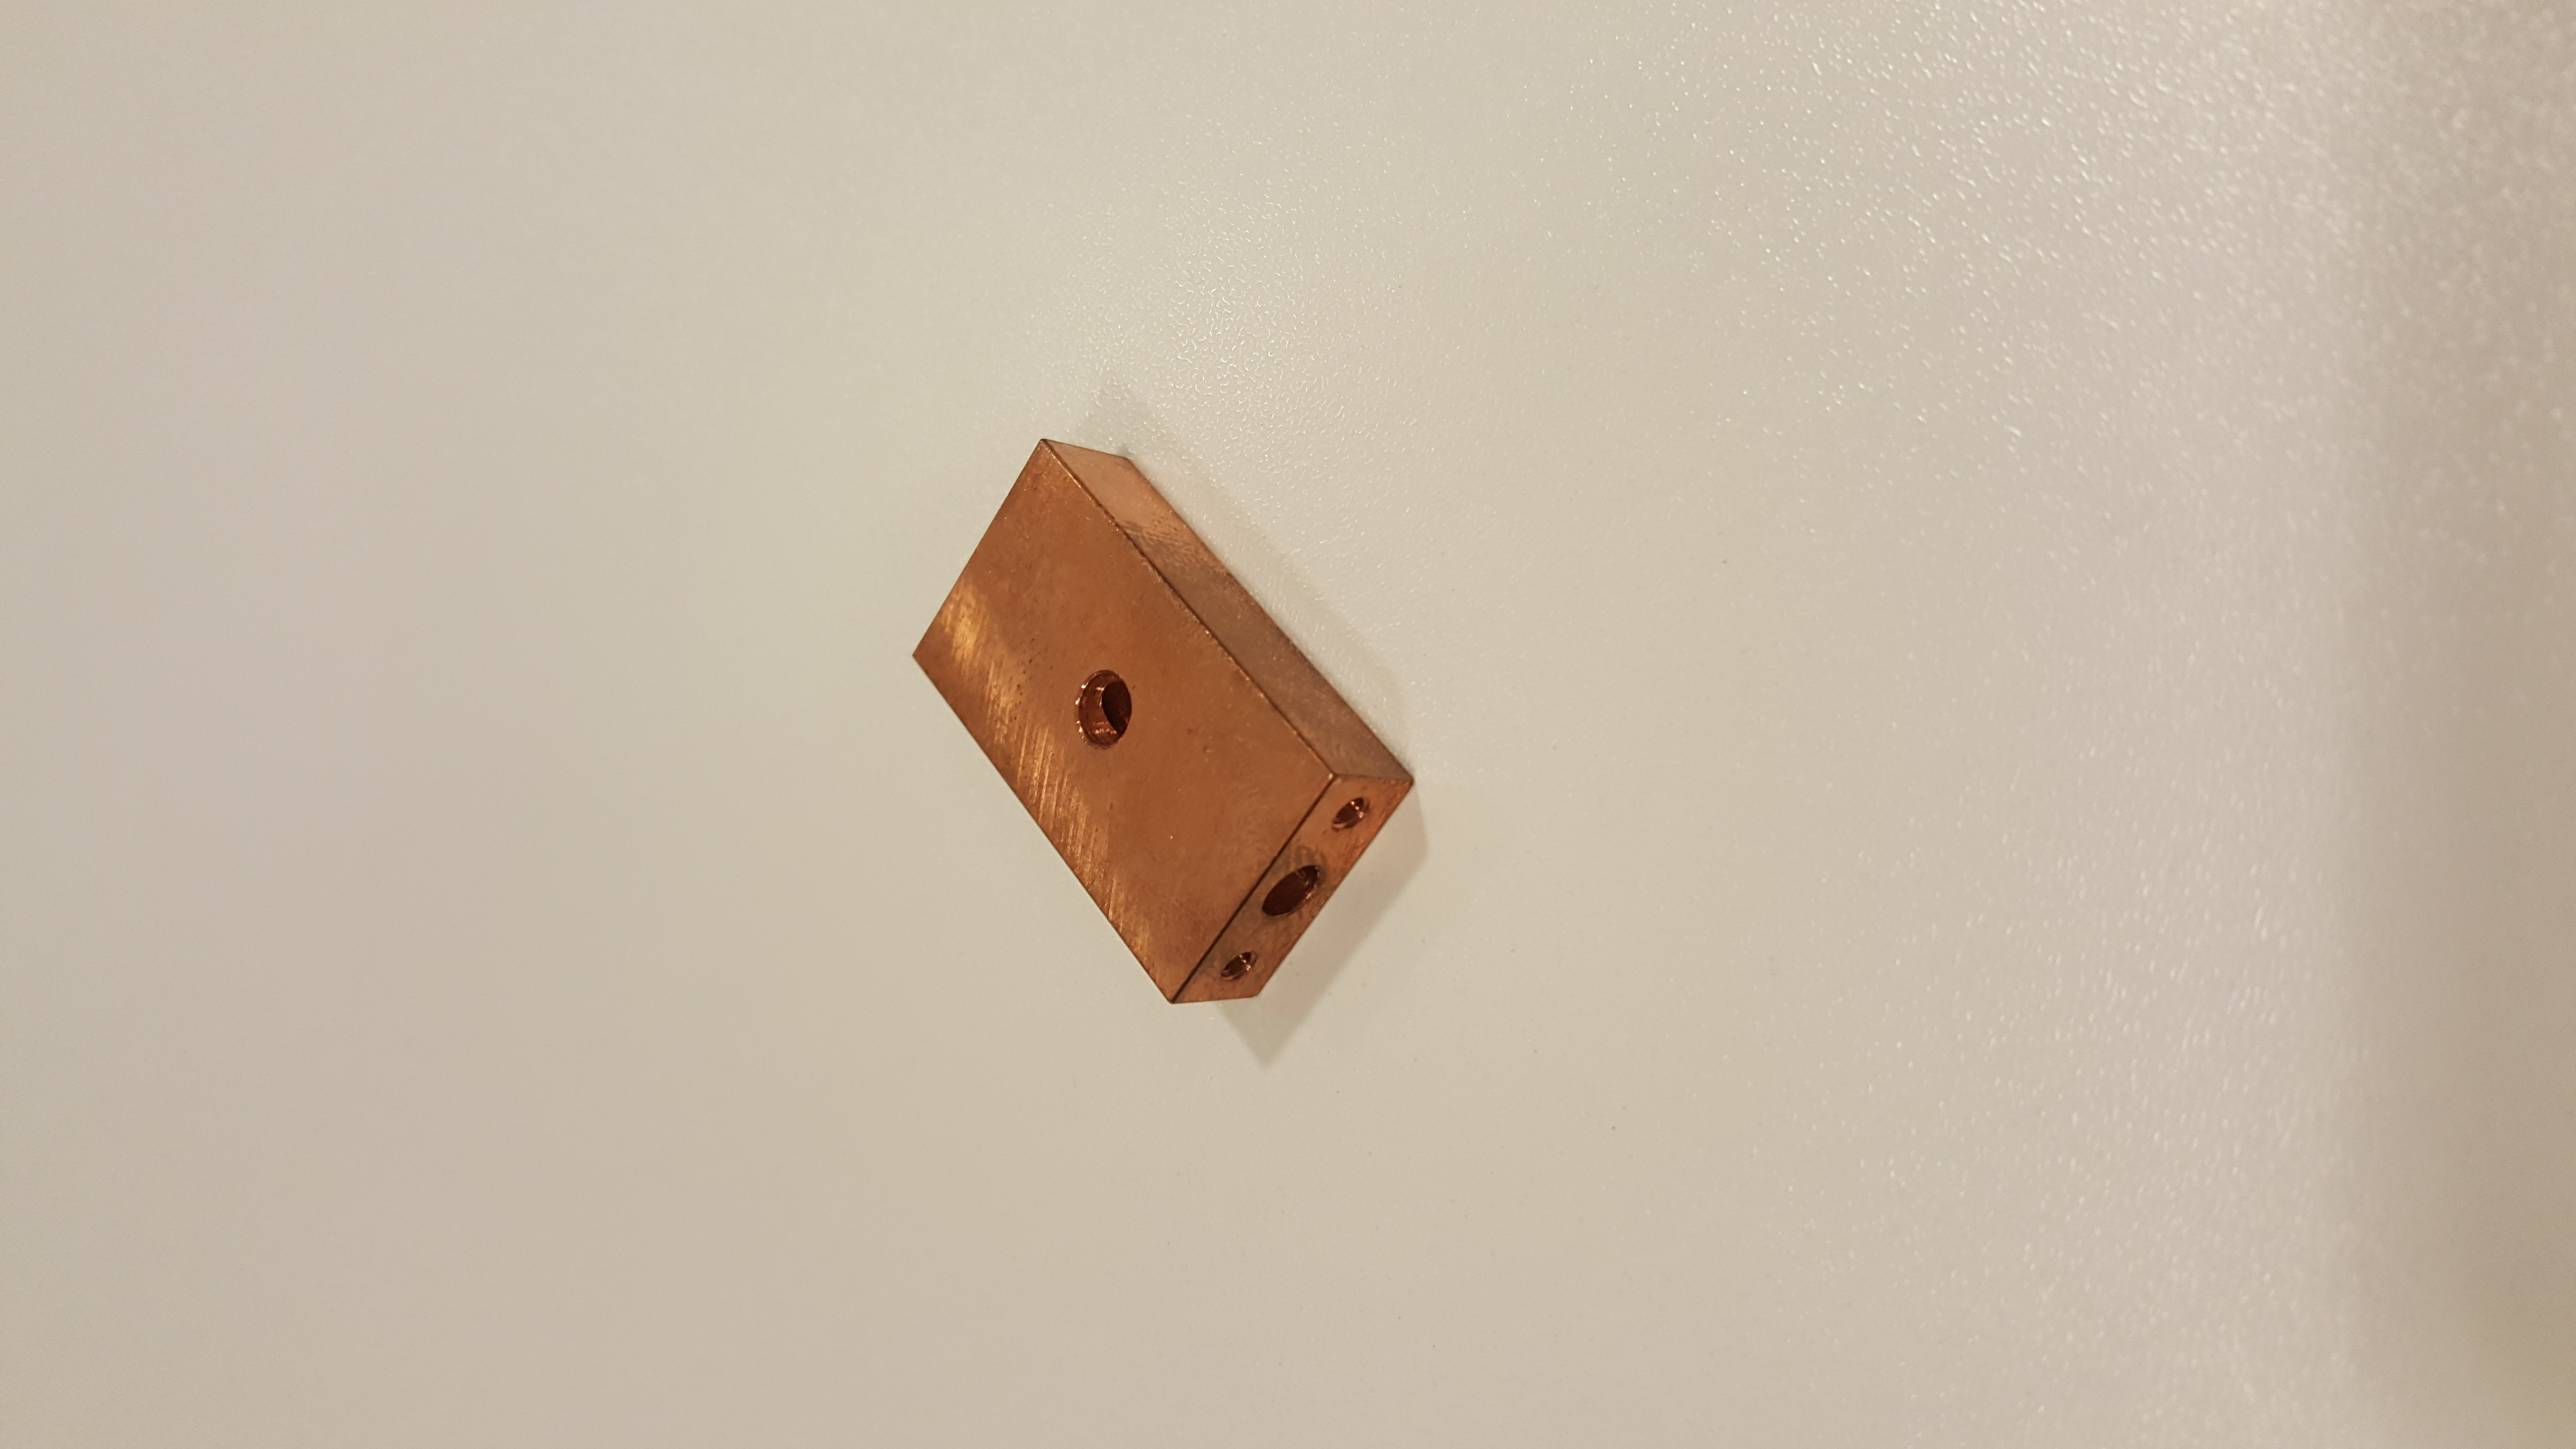
\includegraphics[angle=-90,trim=1550 300 1950 300,clip,width=0.975\linewidth]{figure/Filterbilder/filterbox.jpg}
    \caption{Maskinarbetat kopparblock för att konstruera att distribuerat lågpassfilter.}
    \label{fig:filterbox}
\end{wrapfigure}
I detta projekt har vi konstruerat ett distribuerat lågpassfilter genom att i en koaxial geometri ersätta en del av det isolerande dielektrikum mellan centerledare och hölje med ett dielektrikum med frekvensberoende förluster för att på så sätt effektivt dämpa höga frekvenser.  

De distribuerade lågpassfilter som konstruerats i detta projekt består i huvudsak av tre olika delar: två cylindriska SMA kontakter med en delvis isolerad centerledare, Emerson \& Cuming Stycast 1266 och ett rektangulärt block av maskinarbetad koppar som visas i figur \ref{fig:filterbox}. Från kopparblockets kortsida har ett hål borrats genom hela blocket för att ge plats åt de två SMA kontakterna som ska föras in i kopparblockat från var sin sida och agera som filtrets centerledare. På de båda kortsidorna finns också två skruvhål borrade för att kunna fästa SMA kontakten vid kopparblocket. Från kopparblockets ovansida har ett titthål borrats för att kunna löda ihop de två SMA kontakterna samt för att kunna fylla hålrummet mellan den oisolerade centerledaren och kopparblocket med Stycast som är ett dielektrikum med förluster för att ge filtret en frekvensberoende dämpning som diskuteras i avsnitt \ref{sec:filterdesign}.

\begin{comment}
Om det här blir bra:
- Så här har vi bestämt att göra filtrena - introducera hur de ser ut osv så att man får ett hum om dem
- Varför vi har gjort det (teoriförklaring) - varför valde vi denna metod osv
- Konstruktion av filter - hur vi konstruerade och varför vi gjorde på det sättet
- Mätningar och filterkarakteristik
\end{comment}

\section{Filterdesign}
\label{sec:filterdesign}
För att undersöka egenskaperna hos en transmissionsledning kan man utgå från propagationskonstanten $\gamma =\sqrt{(R+j\omega L)+(G+j\omega C)} $ för en generell transmissionsledning, vilket visas i \ref{app:trans}.

För en koaxial geometri som vårt distribuerade filter är baserad på ges $R, L, G$ och $C$ av
\begin{equation*}
    R=\frac{1}{2\pi}\sqrt{\frac{\pi f\mu_c}{\sigma_c}}\left(\frac{1}{a}+\frac{1}{b}\right),\hspace{1em} L=\frac{\mu}{2\pi}\ln\frac{b}{a},\hspace{1em}G=\frac{2\pi\sigma}{\ln\frac{b}{a}},\hspace{1em}C=\frac{2\pi\epsilon}{\ln\frac{b}{a}}
\end{equation*}
Där $a$ och $b$ är inner- respektive ytterradie, $\mu_c=\mu_r\mu_0$ är ledarens permeabilitet, $\sigma_c$ ledarens konduktivitet, $\sigma$ är dielektrikumets konduktivitet och $\epsilon =\epsilon_r\epsilon_0$ är dielektrikumets permittivitet. 
 

Genom att välja $a=\unit[0,64]{mm}$ och $b=\unit[2,03]{mm}$, vilket motsvarar dimensionerna på vårt filter som konstruerats i detta projekt. Vidare antar vi att ledaren består av koppar vilket ger $\mu_c=\mu_0$ och $\sigma_c=\unit[5,96\cdot 10^7]{S/m}$. Om vi också antar att vårt dielektrikum har $\epsilon=3\epsilon_0$ och en dielektrisk förlusttangent $\delta_e$ som kan relateras till dielektrikumets konduktivitet genom
\begin{equation*}
    \tan\delta_e=\frac{\epsilon^{''}}{\epsilon'}\approx\frac{\sigma}{\omega\epsilon}
\end{equation*}
\autocite{cheng}. Så kan dämpningen som funktion av frekvens och förlusttangent beräknas, vilket visas i \figref{fig:attn_ex}.

\begin{figure}[H]
    
        \centering
        \setlength\figurewidth{0.75\linewidth}
        \setlength\figureheight{12em}
        % This file was created by matlab2tikz.
%
\definecolor{mycolor1}{rgb}{0.20810,0.16630,0.52920}%
\definecolor{mycolor2}{rgb}{0.21162,0.18978,0.57768}%
\definecolor{mycolor3}{rgb}{0.20810,0.23860,0.67709}%
\definecolor{mycolor4}{rgb}{0.19590,0.26446,0.72790}%
\definecolor{mycolor5}{rgb}{0.12527,0.32424,0.83027}%
\definecolor{mycolor6}{rgb}{0.01170,0.38751,0.88196}%
\definecolor{mycolor7}{rgb}{0.00596,0.40861,0.88284}%
\definecolor{mycolor8}{rgb}{0.03285,0.44304,0.87196}%
\definecolor{mycolor9}{rgb}{0.04981,0.45857,0.86406}%
\definecolor{mycolor10}{rgb}{0.07227,0.48867,0.84670}%
\definecolor{mycolor11}{rgb}{0.07935,0.52002,0.83118}%
\definecolor{mycolor12}{rgb}{0.07494,0.53754,0.82627}%
\definecolor{mycolor13}{rgb}{0.04877,0.57722,0.82283}%
\definecolor{mycolor14}{rgb}{0.03434,0.59658,0.81985}%
\definecolor{mycolor15}{rgb}{0.02389,0.62866,0.80376}%
\definecolor{mycolor16}{rgb}{0.02277,0.65349,0.77676}%
\definecolor{mycolor17}{rgb}{0.02666,0.66420,0.76072}%
\definecolor{mycolor18}{rgb}{0.05897,0.68376,0.72539}%
\definecolor{mycolor19}{rgb}{0.08430,0.69283,0.70617}%
\definecolor{mycolor20}{rgb}{0.14527,0.70976,0.66463}%
\definecolor{mycolor21}{rgb}{0.21783,0.72504,0.61926}%
\definecolor{mycolor22}{rgb}{0.25864,0.73171,0.59543}%
\definecolor{mycolor23}{rgb}{0.34817,0.74243,0.54727}%
\definecolor{mycolor24}{rgb}{0.39526,0.74590,0.52444}%
\definecolor{mycolor25}{rgb}{0.48712,0.74906,0.48398}%
\definecolor{mycolor26}{rgb}{0.57086,0.74852,0.44939}%
\definecolor{mycolor27}{rgb}{0.60985,0.74731,0.43369}%
\definecolor{mycolor28}{rgb}{0.68342,0.74348,0.40443}%
\definecolor{mycolor29}{rgb}{0.71841,0.74113,0.39048}%
\definecolor{mycolor30}{rgb}{0.78584,0.73557,0.36327}%
\definecolor{mycolor31}{rgb}{0.85066,0.72990,0.33603}%
\definecolor{mycolor32}{rgb}{0.88243,0.72743,0.32170}%
\definecolor{mycolor33}{rgb}{0.94496,0.72611,0.28864}%
\definecolor{mycolor34}{rgb}{0.97390,0.73140,0.26665}%
\definecolor{mycolor35}{rgb}{0.99904,0.76531,0.21641}%
\definecolor{mycolor36}{rgb}{0.98800,0.80660,0.17937}%
\definecolor{mycolor37}{rgb}{0.97886,0.82714,0.16331}%
\definecolor{mycolor38}{rgb}{0.96259,0.87051,0.13090}%
\definecolor{mycolor39}{rgb}{0.95887,0.89490,0.11324}%
\definecolor{mycolor40}{rgb}{0.96610,0.95144,0.07553}%
\definecolor{mycolor41}{rgb}{0.97630,0.98310,0.05380}%
%
\begin{tikzpicture}[%
trim axis left, trim axis right
]

\begin{axis}[%
width=0.914\figurewidth,
height=\figureheight,
at={(0\figurewidth,0\figureheight)},
scale only axis,
point meta min=0,
point meta max=4.63658963147167,
xmin=0,
xmax=50,
xlabel style={font=\color{white!15!black}},
scaled y ticks = false, 
  scaled x ticks = false, 
  y tick label style={/pgf/number format/.cd, fixed, precision=2},
xlabel={Frekvens (\unit{GHz})},
ymin=0,
ymax=0.06,
ylabel style={font=\color{white!15!black}},
ylabel={Förlusttangent $\delta_e$},
axis background/.style={fill=white},
title style={font=\bfseries},
title={Dämpning som funktion av frekvens och $\delta_e$ (\unit{dB/cm})},
colormap={mymap}{[1pt] rgb(0pt)=(0.2081,0.1663,0.5292); rgb(1pt)=(0.211624,0.189781,0.577676); rgb(2pt)=(0.212252,0.213771,0.626971); rgb(3pt)=(0.2081,0.2386,0.677086); rgb(4pt)=(0.195905,0.264457,0.7279); rgb(5pt)=(0.170729,0.291938,0.779248); rgb(6pt)=(0.125271,0.324243,0.830271); rgb(7pt)=(0.0591333,0.359833,0.868333); rgb(8pt)=(0.0116952,0.38751,0.881957); rgb(9pt)=(0.00595714,0.408614,0.882843); rgb(10pt)=(0.0165143,0.4266,0.878633); rgb(11pt)=(0.0328524,0.443043,0.871957); rgb(12pt)=(0.0498143,0.458571,0.864057); rgb(13pt)=(0.0629333,0.47369,0.855438); rgb(14pt)=(0.0722667,0.488667,0.8467); rgb(15pt)=(0.0779429,0.503986,0.838371); rgb(16pt)=(0.0793476,0.520024,0.831181); rgb(17pt)=(0.0749429,0.537543,0.826271); rgb(18pt)=(0.0640571,0.556986,0.823957); rgb(19pt)=(0.0487714,0.577224,0.822829); rgb(20pt)=(0.0343429,0.596581,0.819852); rgb(21pt)=(0.0265,0.6137,0.8135); rgb(22pt)=(0.0238905,0.628662,0.803762); rgb(23pt)=(0.0230905,0.641786,0.791267); rgb(24pt)=(0.0227714,0.653486,0.776757); rgb(25pt)=(0.0266619,0.664195,0.760719); rgb(26pt)=(0.0383714,0.674271,0.743552); rgb(27pt)=(0.0589714,0.683757,0.725386); rgb(28pt)=(0.0843,0.692833,0.706167); rgb(29pt)=(0.113295,0.7015,0.685857); rgb(30pt)=(0.145271,0.709757,0.664629); rgb(31pt)=(0.180133,0.717657,0.642433); rgb(32pt)=(0.217829,0.725043,0.619262); rgb(33pt)=(0.258643,0.731714,0.595429); rgb(34pt)=(0.302171,0.737605,0.571186); rgb(35pt)=(0.348167,0.742433,0.547267); rgb(36pt)=(0.395257,0.7459,0.524443); rgb(37pt)=(0.44201,0.748081,0.503314); rgb(38pt)=(0.487124,0.749062,0.483976); rgb(39pt)=(0.530029,0.749114,0.466114); rgb(40pt)=(0.570857,0.748519,0.44939); rgb(41pt)=(0.609852,0.747314,0.433686); rgb(42pt)=(0.6473,0.7456,0.4188); rgb(43pt)=(0.683419,0.743476,0.404433); rgb(44pt)=(0.71841,0.741133,0.390476); rgb(45pt)=(0.752486,0.7384,0.376814); rgb(46pt)=(0.785843,0.735567,0.363271); rgb(47pt)=(0.818505,0.732733,0.34979); rgb(48pt)=(0.850657,0.7299,0.336029); rgb(49pt)=(0.882433,0.727433,0.3217); rgb(50pt)=(0.913933,0.725786,0.306276); rgb(51pt)=(0.944957,0.726114,0.288643); rgb(52pt)=(0.973895,0.731395,0.266648); rgb(53pt)=(0.993771,0.745457,0.240348); rgb(54pt)=(0.999043,0.765314,0.216414); rgb(55pt)=(0.995533,0.786057,0.196652); rgb(56pt)=(0.988,0.8066,0.179367); rgb(57pt)=(0.978857,0.827143,0.163314); rgb(58pt)=(0.9697,0.848138,0.147452); rgb(59pt)=(0.962586,0.870514,0.1309); rgb(60pt)=(0.958871,0.8949,0.113243); rgb(61pt)=(0.959824,0.921833,0.0948381); rgb(62pt)=(0.9661,0.951443,0.0755333); rgb(63pt)=(0.9763,0.9831,0.0538)},
colorbar,
colorbar style={ylabel style={font=\color{white!15!black}}, ylabel={Dämpning (\unit{dB/cm})}}
]
\addplot[fill=mycolor1, draw=none, forget plot] table[row sep=crcr] {%
%
x	y\\
0	0\\
0	0.06\\
50	0.06\\
50	0\\
};
\addplot[fill=mycolor2, draw=none, forget plot] table[row sep=crcr] {%
%
x	y\\
1.19144708261184	0.06\\
1.19738768313977	0.0596984924623116\\
1.20338768327065	0.0593969849246231\\
1.20944797907785	0.0590954773869347\\
1.21556948474945	0.0587939698492462\\
1.22175313304829	0.0584924623115578\\
1.22799987578618	0.0581909547738693\\
1.23431068431262	0.0578894472361809\\
1.24068655001872	0.0575879396984925\\
1.24712848485679	0.057286432160804\\
1.25363752187613	0.0569849246231156\\
1.25628140703518	0.05686334586169\\
1.2602203893145	0.0566834170854271\\
1.26687648458241	0.0563819095477387\\
1.27360311848223	0.0560804020100503\\
1.28040141908233	0.0557788944723618\\
1.28727253863366	0.0554773869346734\\
1.29421765422133	0.0551758793969849\\
1.30123796843723	0.0548743718592965\\
1.30833471007471	0.054572864321608\\
1.31550913484608	0.0542713567839196\\
1.3227625261238	0.0539698492462312\\
1.33009619570627	0.0536683417085427\\
1.33751148460929	0.0533668341708543\\
1.34500976388401	0.0530653266331658\\
1.35259243546259	0.0527638190954774\\
1.36026093303254	0.0524623115577889\\
1.36801672294098	0.0521608040201005\\
1.37586130512992	0.0518592964824121\\
1.38379621410394	0.0515577889447236\\
1.39182301993147	0.0512562814070352\\
1.39994332928106	0.0509547738693467\\
1.40815878649412	0.0506532663316583\\
1.41647107469565	0.0503517587939698\\
1.42488191694442	0.0500502512562814\\
1.43339307742441	0.049748743718593\\
1.4420063626791	0.0494472361809045\\
1.45072362289051	0.0491457286432161\\
1.45954675320485	0.0488442211055276\\
1.46847769510683	0.0485427135678392\\
1.47751843784464	0.0482412060301508\\
1.48667101990786	0.0479396984924623\\
1.49593753056057	0.0476381909547739\\
1.50532011143216	0.0473366834170854\\
1.50753768844221	0.0472659690463758\\
1.51483053847589	0.047035175879397\\
1.52446469959388	0.0467336683417085\\
1.5342220141912	0.0464321608040201\\
1.5441048600067	0.0461306532663317\\
1.55411567638543	0.0458291457286432\\
1.56425696628682	0.0455276381909548\\
1.57453129837204	0.0452261306532663\\
1.58494130917404	0.0449246231155779\\
1.59548970535416	0.0446231155778894\\
1.6061792660494	0.044321608040201\\
1.61701284531464	0.0440201005025126\\
1.62799337466417	0.0437185929648241\\
1.63912386571753	0.0434170854271357\\
1.65040741295444	0.0431155778894472\\
1.66184719658428	0.0428140703517588\\
1.67344648553561	0.0425125628140704\\
1.68520864057167	0.0422110552763819\\
1.69713711753812	0.0419095477386935\\
1.70923547074956	0.041608040201005\\
1.72150735652183	0.0413065326633166\\
1.73395653685752	0.0410050251256281\\
1.74658688329234	0.0407035175879397\\
1.75879396984925	0.0404162246635251\\
1.75940311763721	0.0404020100502513\\
1.77242373869309	0.0401005025125628\\
1.7856383130215	0.0397989949748744\\
1.79905120834373	0.0394974874371859\\
1.81266692451788	0.0391959798994975\\
1.82649009857379	0.038894472361809\\
1.84052550998007	0.0385929648241206\\
1.85477808615566	0.0382914572864322\\
1.86925290823929	0.0379899497487437\\
1.88395521713107	0.0376884422110553\\
1.89889041982126	0.0373869346733668\\
1.91406409602232	0.0370854271356784\\
1.92948200512125	0.0367839195979899\\
1.94515009347054	0.0364824120603015\\
1.96107450203697	0.0361809045226131\\
1.97726157442905	0.0358793969849246\\
1.99371786532515	0.0355778894472362\\
2.01005025125628	0.0352835293255505\\
2.01045060202564	0.0352763819095477\\
2.02748531189508	0.0349748743718593\\
2.04481092764453	0.0346733668341709\\
2.06243496729942	0.0343718592964824\\
2.08036521019226	0.034070351758794\\
2.09860970841514	0.0337688442211055\\
2.11717679887977	0.0334673366834171\\
2.13607511602323	0.0331658291457286\\
2.15531360519996	0.0328643216080402\\
2.17490153680364	0.0325628140703518\\
2.19484852116585	0.0322613065326633\\
2.21516452428182	0.0319597989949749\\
2.23585988441726	0.0316582914572864\\
2.25694532965451	0.031356783919598\\
2.26130653266332	0.0312951227091478\\
2.27845040919689	0.0310552763819095\\
2.30037381118384	0.0307537688442211\\
2.32272294316035	0.0304522613065327\\
2.34551033021971	0.0301507537688442\\
2.36874899364345	0.0298492462311558\\
2.39245247571799	0.0295477386934673\\
2.41663486605595	0.0292462311557789\\
2.44131082952928	0.0289447236180905\\
2.46649563593087	0.028643216080402\\
2.49220519149052	0.0283417085427136\\
2.51256281407035	0.0281073402809218\\
2.51846205374525	0.0280402010050251\\
2.54529910564829	0.0277386934673367\\
2.57271398145867	0.0274371859296482\\
2.60072554906018	0.0271356783919598\\
2.6293535068422	0.0268341708542714\\
2.65861842990345	0.0265326633165829\\
2.68854181937508	0.0262311557788945\\
2.71914615511145	0.025929648241206\\
2.75045495202007	0.0256281407035176\\
2.76381909547739	0.0255015213418109\\
2.78251097808253	0.0253266331658291\\
2.8153361647545	0.0250251256281407\\
2.84894474561017	0.0247236180904523\\
2.88336510765884	0.0244221105527638\\
2.91862702618409	0.0241206030150754\\
2.95476175066164	0.0238190954773869\\
2.99180209713798	0.0235175879396985\\
3.01507537688442	0.0233319319646328\\
3.0297962208315	0.0232160804020101\\
3.06878989043818	0.0229145728643216\\
3.10879999155776	0.0226130653266332\\
3.1498667961335	0.0223115577889447\\
3.19203273206372	0.0220100502512563\\
3.23534252943252	0.0217085427135678\\
3.26633165829146	0.0214977128820055\\
3.27985544557273	0.0214070351758794\\
3.3256387581825	0.021105527638191\\
3.37271795133392	0.0208040201005025\\
3.42114883967993	0.0205025125628141\\
3.47099048987355	0.0202010050251256\\
3.51758793969849	0.0199268486897893\\
3.52230951177666	0.0198994974874372\\
3.57521024482622	0.0195979899497487\\
3.62972379678728	0.0192964824120603\\
3.68592507256014	0.0189949748743719\\
3.74389368844046	0.0186934673366834\\
3.76884422110553	0.0185665483797922\\
3.80374352227727	0.018391959798995\\
3.86555941841805	0.0180904522613065\\
3.92941723514808	0.0177889447236181\\
3.99541985324477	0.0174874371859296\\
4.02010050251256	0.0173772356264787\\
4.0637125611641	0.0171859296482412\\
4.13440110722996	0.0168844221105528\\
4.20759196912306	0.0165829145728643\\
4.2713567839196	0.0163286581424394\\
4.28342985187836	0.0162814070351759\\
4.36210385885606	0.0159798994974874\\
4.44372144840149	0.015678391959799\\
4.52261306532663	0.0153972960938412\\
4.52845541270617	0.0153768844221106\\
4.61654654648982	0.0150753768844221\\
4.70813236761436	0.0147738693467337\\
4.77386934673367	0.0145645888136097\\
4.80344701374683	0.0144723618090452\\
4.90275197945635	0.0141708542713568\\
5.00624904521435	0.0138693467336683\\
5.0251256281407	0.0138156943736133\\
5.1142746929213	0.0135678391959799\\
5.22707930678402	0.0132663316582915\\
5.27638190954774	0.0131386021610315\\
5.34502062404188	0.012964824120603\\
5.4684441090918	0.0126633165829146\\
5.52763819095477	0.012523489740029\\
5.59775047828075	0.0123618090452261\\
5.73336367569118	0.0120603015075377\\
5.77889447236181	0.011962245940413\\
5.87577639730737	0.0117587939698492\\
6.02547706429209	0.0114572864321608\\
6.03015075376884	0.0114481142367967\\
6.18310776196582	0.0111557788944724\\
6.28140703517588	0.0109754209186448\\
6.3492544381856	0.0108542713567839\\
6.52464560942723	0.0105527638190955\\
6.53266331658291	0.0105393678278719\\
6.71011673760541	0.010251256281407\\
6.78391959798995	0.0101358682451066\\
6.90652340295676	0.00994974874371859\\
7.03517587939699	0.00976142135650928\\
7.11487402077697	0.00964824120603015\\
7.28643216080402	0.00941300993708437\\
7.33630285664084	0.00934673366834171\\
7.53768844221106	0.00908802003681321\\
7.57209065477433	0.00904522613065327\\
7.78894472361809	0.00878417582566944\\
7.82368938848184	0.00874371859296482\\
8.04020100502513	0.00849948667063796\\
8.09275214283101	0.00844221105527638\\
8.29145728643216	0.00823220384751422\\
8.381169428976	0.00814070351758794\\
8.5427135678392	0.00798078490185705\\
8.69111361634566	0.0078391959798995\\
8.79396984924623	0.00774386412769402\\
9.02509369119449	0.00753768844221106\\
9.04522613065327	0.00752022797317139\\
9.2964824120603	0.0073087942387001\\
9.38607159958015	0.00723618090452261\\
9.54773869346734	0.00710859527805195\\
9.7774298138411	0.00693467336683417\\
9.79899497487437	0.00691876289903991\\
10.0502512562814	0.00673851566243767\\
10.2032410233303	0.00663316582914573\\
10.3015075376884	0.00656714906011637\\
10.5527638190955	0.00640402553679226\\
10.668256235396	0.00633165829145729\\
10.8040201005025	0.00624856716208302\\
11.0552763819095	0.00610024869074023\\
11.1781976265052	0.00603015075376884\\
11.3065326633166	0.00595859168186289\\
11.5577889447236	0.00582315943888854\\
11.7399464279691	0.0057286432160804\\
11.8090452261307	0.00569355261828722\\
12.0603015075377	0.00556940506700923\\
12.3115577889447	0.00545038093666964\\
12.3618783530845	0.00542713567839196\\
12.5628140703518	0.00533617095554996\\
12.8140703517588	0.00522649051575634\\
13.0542752415156	0.00512562814070352\\
13.0653266331658	0.00512107687691314\\
13.3165829145729	0.00501968697824391\\
13.5678391959799	0.00492209619281831\\
13.8190954773869	0.00482809610354931\\
13.8299317986984	0.00482412060301507\\
14.070351758794	0.00473749307260093\\
14.321608040201	0.00465010740836499\\
14.572864321608	0.00456577171552544\\
14.7049428362564	0.00452261306532663\\
14.8241206030151	0.00448432991573429\\
15.0753768844221	0.00440563643291287\\
15.3266331658291	0.00432955535096162\\
15.5778894472362	0.00425595948538995\\
15.699829167534	0.00422110552763819\\
15.8291457286432	0.00418472969853081\\
16.0804020100503	0.00411575438902366\\
16.3316582914573	0.00404892890061484\\
16.5829145728643	0.0039841548914309\\
16.8341708542714	0.00392133991390569\\
16.8412498433564	0.00391959798994975\\
17.0854271356784	0.00386039689075257\\
17.3366834170854	0.00380124398664834\\
17.5879396984925	0.00374380397958686\\
17.8391959798995	0.00368800401333851\\
18.0904522613065	0.00363377529586178\\
18.1644782926466	0.00361809045226131\\
18.3417085427136	0.00358105276843888\\
18.5929648241206	0.00352977498444054\\
18.8442211055276	0.00347988377983697\\
19.0954773869347	0.00343132404407903\\
19.3467336683417	0.0033840435417091\\
19.5979899497487	0.00333799272751441\\
19.7170840615942	0.00331658291457286\\
19.8492462311558	0.00329312454569962\\
20.1005025125628	0.00324939433614328\\
20.3517587939699	0.0032067596773177\\
20.6030150753769	0.00316518020008911\\
20.8542713567839	0.00312461748947326\\
21.105527638191	0.00308503496795772\\
21.356783919598	0.00304639778707913\\
21.5649815913313	0.00301507537688442\\
21.608040201005	0.00300867271911632\\
21.8592964824121	0.00297182805012771\\
22.1105527638191	0.00293583357757446\\
22.3618090452261	0.00290066042772744\\
22.6130653266332	0.00286628101610183\\
22.8643216080402	0.00283266897639066\\
23.1155778894472	0.00279979909404426\\
23.3668341708543	0.00276764724414522\\
23.6180904522613	0.00273619033325861\\
23.8022134030735	0.00271356783919598\\
23.8693467336683	0.00270540623638563\\
24.1206030150754	0.00267527374855598\\
24.3718592964824	0.00264577258113461\\
24.6231155778894	0.00261688325482595\\
24.8743718592965	0.00258858708123469\\
25.1256281407035	0.00256086612318603\\
25.3768844221106	0.00253370315740924\\
25.6281407035176	0.00250708163942179\\
25.8793969849246	0.00248098567046437\\
26.1306532663317	0.00245539996634846\\
26.3819095477387	0.00243030982808858\\
26.5677807461779	0.00241206030150754\\
26.6331658291457	0.0024057011082499\\
26.8844221105528	0.00238156018602115\\
27.1356783919598	0.00235787397501731\\
27.3869346733668	0.00233462985511843\\
27.6381909547739	0.00231181566750198\\
27.8894472361809	0.00228941969378868\\
28.1407035175879	0.00226743063630857\\
28.391959798995	0.00224583759941765\\
28.643216080402	0.00222463007180056\\
28.894472361809	0.0022037979096992\\
29.1457286432161	0.00218333132101106\\
29.3969849246231	0.00216322085020542\\
29.6482412060302	0.00214345736400856\\
29.8994974874372	0.00212403203781273\\
30.0764170607754	0.0021105527638191\\
30.1507537688442	0.00210493633815767\\
30.4020100502513	0.00208616201349474\\
30.6532663316583	0.00206770110134391\\
30.9045226130653	0.00204954588889671\\
31.1557788944724	0.00203168891352523\\
31.4070351758794	0.00201412295273636\\
31.6582914572864	0.00199684101460572\\
31.9095477386935	0.00197983632866488\\
32.1608040201005	0.00196310233721692\\
32.4120603015075	0.00194663268705719\\
32.6633165829146	0.00193042122157715\\
32.9145728643216	0.00191446197323112\\
33.1658291457286	0.00189874915634631\\
33.4170854271357	0.00188327716025821\\
33.6683417085427	0.00186804054275434\\
33.9195979899498	0.00185303402381013\\
34.1708542713568	0.00183825247960211\\
34.4221105527638	0.00182369093678397\\
34.6733668341709	0.00180934456701236\\
34.6786499532893	0.00180904522613065\\
34.9246231155779	0.00179520867195196\\
35.1758793969849	0.00178127870747277\\
35.427135678392	0.00176755024991401\\
35.678391959799	0.00175401900076446\\
35.929648241206	0.00174068078247213\\
36.1809045226131	0.00172753153422683\\
36.4321608040201	0.0017145673079177\\
36.6834170854271	0.0017017842642575\\
36.9346733668342	0.00168917866906549\\
37.1859296482412	0.00167674688970152\\
37.4371859296482	0.00166448539164419\\
37.6884422110553	0.00165239073520624\\
37.9396984924623	0.00164045957238098\\
38.1909547738694	0.0016286886438135\\
38.4422110552764	0.00161707477589109\\
38.6934673366834	0.00160561487794736\\
38.9447236180905	0.00159430593957494\\
39.1959798994975	0.00158314502804189\\
39.4472361809045	0.00157212928580718\\
39.6984924623116	0.00156125592813073\\
39.9497487437186	0.00155052224077407\\
40.2010050251256	0.00153992557778741\\
40.4522613065327	0.00152946335937949\\
40.7035175879397	0.00151913306986656\\
40.9547738693467	0.00150893225569713\\
40.9893739014053	0.00150753768844221\\
41.2060301507538	0.001498858518431\\
41.4572864321608	0.00148890952751302\\
41.7085427135678	0.00147908300546785\\
41.9597989949749	0.0014693767289239\\
42.2110552763819	0.00145978852779369\\
42.462311557789	0.0014503162836902\\
42.713567839196	0.00144095792839937\\
42.964824120603	0.00143171144240632\\
43.2160804020101	0.0014225748534732\\
43.4673366834171	0.00141354623526645\\
43.7185929648241	0.00140462370603168\\
43.9698492462312	0.00139580542731405\\
44.2211055276382	0.00138708960272245\\
44.4723618090452	0.00137847447673569\\
44.7236180904523	0.00136995833354915\\
44.9748743718593	0.00136153949596014\\
45.2261306532663	0.00135321632429058\\
45.4773869346734	0.00134498721534553\\
45.7286432160804	0.00133685060140611\\
45.9798994974874	0.00132880494925569\\
46.2311557788945	0.00132084875923778\\
46.4824120603015	0.00131298056434471\\
46.7336683417085	0.00130519892933576\\
46.9849246231156	0.00129750244988369\\
47.2361809045226	0.00128988975174861\\
47.4874371859297	0.00128235948997817\\
47.7386934673367	0.00127491034813311\\
47.9899497487437	0.0012675410375372\\
48.2412060301508	0.00126025029655072\\
48.4924623115578	0.00125303688986662\\
48.7437185929648	0.00124589960782851\\
48.9949748743719	0.00123883726576972\\
49.2462311557789	0.00123184870337263\\
49.4974874371859	0.00122493278404769\\
49.748743718593	0.00121808839433117\\
50	0.0012113144433013\\
50 0.06\\
};
\addplot[fill=mycolor3, draw=none, forget plot] table[row sep=crcr] {%
%
x	y\\
2.40219578298825	0.06\\
2.41422678354209	0.0596984924623116\\
2.42637862390151	0.0593969849246231\\
2.43865313524736	0.0590954773869347\\
2.45105218594738	0.0587939698492462\\
2.46357768250499	0.0584924623115578\\
2.4762315705373	0.0581909547738693\\
2.4890158357833	0.0578894472361809\\
2.50193250514349	0.0575879396984925\\
2.51256281407035	0.057342121654408\\
2.51498486240281	0.057286432160804\\
2.52817924871496	0.0569849246231156\\
2.5415125182183	0.0566834170854271\\
2.55498687687809	0.0563819095477387\\
2.56860457762645	0.0560804020100503\\
2.58236792161898	0.0557788944723618\\
2.59627925953195	0.0554773869346734\\
2.61034099290169	0.0551758793969849\\
2.62455557550752	0.0548743718592965\\
2.63892551480015	0.054572864321608\\
2.65345337337723	0.0542713567839196\\
2.66814177050776	0.0539698492462312\\
2.68299338370743	0.0536683417085427\\
2.69801095036674	0.0533668341708543\\
2.71319726943407	0.0530653266331658\\
2.72855520315586	0.0527638190954774\\
2.74408767887612	0.0524623115577889\\
2.75979769089769	0.0521608040201005\\
2.76381909547739	0.0520841744479628\\
2.77569399871199	0.0518592964824121\\
2.79177613586826	0.0515577889447236\\
2.80804539509741	0.0512562814070352\\
2.82450506326624	0.0509547738693467\\
2.84115850467489	0.0506532663316583\\
2.85800916335058	0.0503517587939698\\
2.87506056542342	0.0500502512562814\\
2.89231632158766	0.049748743718593\\
2.90978012965202	0.0494472361809045\\
2.92745577718286	0.0491457286432161\\
2.94534714424419	0.0488442211055276\\
2.96345820623871	0.0485427135678392\\
2.9817930368541	0.0482412060301508\\
3.00035581111936	0.0479396984924623\\
3.01507537688442	0.0477032494660372\\
3.01915267569115	0.0476381909547739\\
3.03819306953437	0.0473366834170854\\
3.05747479579428	0.047035175879397\\
3.07700247423014	0.0467336683417085\\
3.09678084327136	0.0464321608040201\\
3.11681476385261	0.0461306532663317\\
3.13710922339853	0.0458291457286432\\
3.15766933996506	0.0455276381909548\\
3.17850036654453	0.0452261306532663\\
3.19960769554209	0.0449246231155779\\
3.22099686343159	0.0446231155778894\\
3.24267355559928	0.044321608040201\\
3.26464361138426	0.0440201005025126\\
3.26633165829146	0.0439971018847087\\
3.28692213399251	0.0437185929648241\\
3.30950719497756	0.0434170854271357\\
3.33240439466992	0.0431155778894472\\
3.35562025168251	0.0428140703517588\\
3.37916146741099	0.0425125628140704\\
3.40303493248549	0.0422110552763819\\
3.4272477334977	0.0419095477386935\\
3.45180716001685	0.041608040201005\\
3.47672071190936	0.0413065326633166\\
3.50199610697752	0.0410050251256281\\
3.51758793969849	0.0408211897853852\\
3.52764556040922	0.0407035175879397\\
3.5536798770147	0.0404020100502513\\
3.58010091197074	0.0401005025125628\\
3.60691734942145	0.0397989949748744\\
3.6341381354866	0.0394974874371859\\
3.66177248821551	0.0391959798994975\\
3.68982990799824	0.038894472361809\\
3.71832018845884	0.0385929648241206\\
3.7472534278568	0.0382914572864322\\
3.76884422110553	0.0380694768817621\\
3.77664323904769	0.0379899497487437\\
3.80650633741598	0.0376884422110553\\
3.83684503466746	0.0373869346733668\\
3.86767078712239	0.0370854271356784\\
3.89899542202874	0.0367839195979899\\
3.93083115269692	0.0364824120603015\\
3.96319059438156	0.0361809045226131\\
3.99608678095381	0.0358793969849246\\
4.02010050251256	0.0356624138057823\\
4.02953693084631	0.0355778894472362\\
4.06356113281674	0.0352763819095477\\
4.09816433896907	0.0349748743718593\\
4.13336145994389	0.0346733668341709\\
4.16916792279062	0.0343718592964824\\
4.20559969351919	0.034070351758794\\
4.24267330084377	0.0337688442211055\\
4.2713567839196	0.033539159089199\\
4.28040934981858	0.0334673366834171\\
4.31883356552484	0.0331658291457286\\
4.35795338107753	0.0328643216080402\\
4.39778786245531	0.0325628140703518\\
4.43835677884447	0.0322613065326633\\
4.479680635361	0.0319597989949749\\
4.52178070761704	0.0316582914572864\\
4.52261306532663	0.0316523868885027\\
4.56469495554725	0.031356783919598\\
4.60843136444303	0.0310552763819095\\
4.6530134651689	0.0307537688442211\\
4.69846603102427	0.0304522613065327\\
4.74481481244627	0.0301507537688442\\
4.77386934673367	0.0299647317636967\\
4.79209324344717	0.0298492462311558\\
4.8403337301887	0.0295477386934673\\
4.88955477678639	0.0292462311557789\\
4.93978659304119	0.0289447236180905\\
4.99106064259773	0.028643216080402\\
5.0251256281407	0.0284463029090656\\
5.0434162222242	0.0283417085427136\\
5.09689379252309	0.0280402010050251\\
5.15151701913774	0.0277386934673367\\
5.20732312245134	0.0274371859296482\\
5.26435095279925	0.0271356783919598\\
5.27638190954774	0.0270729022994019\\
5.32265724942494	0.0268341708542714\\
5.38227330598113	0.0265326633165829\\
5.4432393165457	0.0262311557788945\\
5.50560166625627	0.025929648241206\\
5.52763819095477	0.0258247324363757\\
5.56942314088589	0.0256281407035176\\
5.63474875696457	0.0253266331658291\\
5.70162435872741	0.0250251256281407\\
5.77010578136796	0.0247236180904523\\
5.77889447236181	0.0246854405874949\\
5.84027211530099	0.0244221105527638\\
5.91216831964082	0.0241206030150754\\
5.98585604486983	0.0238190954773869\\
6.03015075376884	0.0236413995640077\\
6.06141329654959	0.0235175879396985\\
6.13891669206392	0.0232160804020101\\
6.21842701628378	0.0229145728643216\\
6.28140703517588	0.0226811647035142\\
6.30002919018641	0.0226130653266332\\
6.38382166980178	0.0223115577889447\\
6.46987238707927	0.0220100502512563\\
6.53266331658291	0.0217950521079953\\
6.55828190675696	0.0217085427135678\\
6.64916081402426	0.0214070351758794\\
6.74259297809133	0.021105527638191\\
6.78391959798995	0.0209748138829801\\
6.83870444237643	0.0208040201005025\\
6.93760805862447	0.0205025125628141\\
7.03517587939699	0.0202133814119066\\
7.03941487460122	0.0202010050251256\\
7.1442839973814	0.0198994974874372\\
7.25232409665902	0.0195979899497487\\
7.28643216080402	0.0195046608019658\\
7.3637042842705	0.0192964824120603\\
7.47856876163639	0.0189949748743719\\
7.53768844221106	0.0188433725649571\\
7.59709002205336	0.0186934673366834\\
7.71944572783736	0.018391959798995\\
7.78894472361809	0.0182249183774923\\
7.84582264744112	0.0180904522613065\\
7.97642644108207	0.0177889447236181\\
8.04020100502513	0.0176452752801082\\
8.11147127708891	0.0174874371859296\\
8.25118572488346	0.0171859296482412\\
8.29145728643216	0.0171009085050822\\
8.39582582198713	0.0168844221105528\\
8.5427135678392	0.0165886995830317\\
8.5456391011827	0.0165829145728643\\
8.70093734709264	0.0162814070351759\\
8.79396984924623	0.0161058862299115\\
8.86200191737798	0.0159798994974874\\
9.02916760026538	0.015678391959799\\
9.04522613065327	0.0156500146086929\\
9.20280261080308	0.0153768844221106\\
9.2964824120603	0.0152188951512035\\
9.38327319711081	0.0150753768844221\\
9.54773869346734	0.0148105701701554\\
9.57099478189254	0.0147738693467337\\
9.76642498392535	0.0144723618090452\\
9.79899497487437	0.0144232820892024\\
9.97004582034499	0.0141708542713568\\
10.0502512562814	0.0140554497676382\\
10.182379656286	0.0138693467336683\\
10.3015075376884	0.013705646563644\\
10.4040009730207	0.0135678391959799\\
10.5527638190955	0.013372581715029\\
10.6355355241446	0.0132663316582915\\
10.8040201005025	0.0130550847049906\\
10.8776662310552	0.012964824120603\\
11.0552763819095	0.0127520915835578\\
11.1311399047959	0.0126633165829146\\
11.3065326633166	0.0124626331142664\\
11.3967749336046	0.0123618090452261\\
11.5577889447236	0.0121858244681417\\
11.6754701028533	0.0120603015075377\\
11.8090452261307	0.0119208562343983\\
11.9682147476293	0.0117587939698492\\
12.0603015075377	0.0116669865557141\\
12.2761004796033	0.0114572864321608\\
12.3115577889447	0.0114235342273242\\
12.5628140703518	0.0111898724802299\\
12.6003432926703	0.0111557788944724\\
12.8140703517588	0.0109654238884492\\
12.94228582372	0.0108542713567839\\
13.0653266331658	0.01074965568817\\
13.303409721508	0.0105527638190955\\
13.3165829145729	0.0105420752513351\\
13.5678391959799	0.0103422261435264\\
13.6854024525262	0.010251256281407\\
13.8190954773869	0.010149685814671\\
14.070351758794	0.00996406165201842\\
14.090109531254	0.00994974874371859\\
14.321608040201	0.00978498830937611\\
14.5196454163198	0.00964824120603015\\
14.572864321608	0.00961212639300402\\
14.8241206030151	0.00944515883621226\\
14.9763656219617	0.00934673366834171\\
15.0753768844221	0.00928379029989878\\
15.3266331658291	0.0091277444798506\\
15.462943388325	0.00904522613065327\\
15.5778894472362	0.00897676314491091\\
15.8291457286432	0.00883060435135941\\
15.9824174932837	0.00874371859296482\\
16.0804020100503	0.0086890414366752\\
16.3316582914573	0.00855186152494006\\
16.53825147945	0.00844221105527638\\
16.5829145728643	0.00841886496721249\\
16.8341708542714	0.00828986359090566\\
17.0854271356784	0.00816468091517936\\
17.1344204656857	0.00814070351758794\\
17.3366834170854	0.00804315007542883\\
17.5879396984925	0.00792511428543075\\
17.7754943896932	0.0078391959798995\\
17.8391959798995	0.00781042537205997\\
18.0904522613065	0.00769894326047766\\
18.3417085427136	0.00759053597533655\\
18.4667650329767	0.00753768844221106\\
18.5929648241206	0.00748507829578566\\
18.8442211055276	0.0073824518437646\\
19.0954773869347	0.00728254462902211\\
19.2143897120354	0.00723618090452261\\
19.3467336683417	0.00718525020673024\\
19.5979899497487	0.00709046775512797\\
19.8492462311558	0.00699810167728121\\
20.0255817341218	0.00693467336683417\\
20.1005025125628	0.00690806097444877\\
20.3517587939699	0.00682025912681093\\
20.6030150753769	0.00673461409865398\\
20.8542713567839	0.00665104765677806\\
20.9088437347595	0.00663316582914573\\
21.105527638191	0.00656948514044216\\
21.356783919598	0.00648985568443255\\
21.608040201005	0.00641209165684057\\
21.8592964824121	0.00633612849907458\\
21.8742669280741	0.00633165829145729\\
22.1105527638191	0.00626190442513009\\
22.3618090452261	0.00618936075490924\\
22.6130653266332	0.00611844127834636\\
22.8643216080402	0.00604909225149543\\
22.9339334869374	0.00603015075376884\\
23.1155778894472	0.00598126215998378\\
23.3668341708543	0.00591490189024505\\
23.6180904522613	0.00584996439778312\\
23.8693467336683	0.00578640458182072\\
24.1024021251143	0.0057286432160804\\
24.1206030150754	0.00572417921545655\\
24.3718592964824	0.00566324675420224\\
24.6231155778894	0.00560356758865574\\
24.8743718592965	0.00554510359241153\\
25.1256281407035	0.00548781816780476\\
25.3768844221106	0.00543167617010372\\
25.3974279261283	0.00542713567839196\\
25.6281407035176	0.00537664373150994\\
25.8793969849246	0.00532268850078337\\
26.1306532663317	0.00526977928964599\\
26.3819095477387	0.00521788609183938\\
26.6331658291457	0.00516698003623992\\
26.8408488872879	0.00512562814070352\\
26.8844221105528	0.00511703331689031\\
27.1356783919598	0.00506801911416475\\
27.3869346733668	0.00501991173610295\\
27.6381909547739	0.00497268634933511\\
27.8894472361809	0.00492631901767501\\
28.1407035175879	0.00488078666199585\\
28.391959798995	0.00483606702223942\\
28.4598520400987	0.00482412060301507\\
28.643216080402	0.00479213856245264\\
28.894472361809	0.00474898059300358\\
29.1457286432161	0.00470657312450826\\
29.3969849246231	0.00466489683150204\\
29.6482412060302	0.0046239330453512\\
29.8994974874372	0.00458366372660426\\
30.1507537688442	0.00454407143872757\\
30.2887236840897	0.00452261306532663\\
30.4020100502513	0.0045051392929224\\
30.6532663316583	0.00446685097906688\\
30.9045226130653	0.00442919076155562\\
31.1557788944724	0.0043921433778442\\
31.4070351758794	0.00435569405512028\\
31.6582914572864	0.00431982849083288\\
31.9095477386935	0.00428453283414284\\
32.1608040201005	0.00424979366824409\\
32.3713282233241	0.00422110552763819\\
32.4120603015075	0.00421559798461263\\
32.6633165829146	0.00418193314814193\\
32.9145728643216	0.00414878699238688\\
33.1658291457286	0.0041161476756857\\
33.4170854271357	0.0040840037135199\\
33.6683417085427	0.00405234396516187\\
33.9195979899498	0.00402115762091678\\
34.1708542713568	0.00399043418992823\\
34.4221105527638	0.00396016348851865\\
34.6733668341709	0.00393033562903749\\
34.7647287081822	0.00391959798994975\\
34.9246231155779	0.00390094098119377\\
35.1758793969849	0.00387197023036389\\
35.427135678392	0.00384341433086937\\
35.678391959799	0.00381526447692363\\
35.929648241206	0.00378751210977698\\
36.1809045226131	0.00376014890912141\\
36.4321608040201	0.00373316678485164\\
36.6834170854271	0.00370655786916524\\
36.9346733668342	0.00368031450898576\\
37.1859296482412	0.00365442925869341\\
37.4371859296482	0.003628894873149\\
37.5445401178901	0.00361809045226131\\
37.6884422110553	0.00360370428105602\\
37.9396984924623	0.00357885062384787\\
38.1909547738694	0.00355432723366899\\
38.4422110552764	0.00353012760293141\\
38.6934673366834	0.00350624539359025\\
38.9447236180905	0.00348267443166294\\
39.1959798994975	0.00345940870195964\\
39.4472361809045	0.00343644234301536\\
39.6984924623116	0.00341376964221476\\
39.9497487437186	0.00339138503110136\\
40.2010050251256	0.00336928308086276\\
40.4522613065327	0.00334745849798455\\
40.7035175879397	0.00332590612006531\\
40.8131907328085	0.00331658291457286\\
40.9547738693467	0.00330462089657526\\
41.2060301507538	0.00328359791908597\\
41.4572864321608	0.00326283240678551\\
41.7085427135678	0.00324231968285811\\
41.9597989949749	0.00322205518286371\\
42.2110552763819	0.0032020344513861\\
42.462311557789	0.00318225313880016\\
42.713567839196	0.00316270699815344\\
42.964824120603	0.00314339188215728\\
43.2160804020101	0.00312430374028315\\
43.4673366834171	0.00310543861595982\\
43.7185929648241	0.00308679264386729\\
43.9698492462312	0.00306836204732379\\
44.2211055276382	0.00305014313576184\\
44.4723618090452	0.00303213230229019\\
44.7129870658779	0.00301507537688442\\
44.7236180904523	0.00301432602047089\\
44.9748743718593	0.00299672082514216\\
45.2261306532663	0.00297931336635196\\
45.4773869346734	0.00296210034912739\\
45.7286432160804	0.00294507855115356\\
45.9798994974874	0.0029282448207838\\
46.2311557788945	0.0029115960751149\\
46.4824120603015	0.00289512929812479\\
46.7336683417085	0.0028788415388705\\
46.9849246231156	0.00286272990974398\\
47.2361809045226	0.00284679158478366\\
47.4874371859297	0.00283102379803981\\
47.7386934673367	0.00281542384199151\\
47.9899497487437	0.00279998906601346\\
48.2412060301508	0.00278471687489081\\
48.4924623115578	0.00276960472738024\\
48.7437185929648	0.00275465013481561\\
48.9949748743719	0.00273985065975658\\
49.2462311557789	0.0027252039146787\\
49.4477091853894	0.00271356783919598\\
49.4974874371859	0.00271070755772198\\
49.748743718593	0.00269635928843007\\
50	0.00268215687368655\\
50 0.06\\
};
\addplot[fill=mycolor4, draw=none, forget plot] table[row sep=crcr] {%
%
x	y\\
3.61621873052112	0.06\\
3.63436399758791	0.0596984924623116\\
3.6526918619538	0.0593969849246231\\
3.67120509592271	0.0590954773869347\\
3.68990652820508	0.0587939698492462\\
3.70879904535972	0.0584924623115578\\
3.72788559328022	0.0581909547738693\\
3.74716917872744	0.0578894472361809\\
3.76665287090962	0.0575879396984925\\
3.76884422110553	0.0575542231351442\\
3.78634458139141	0.057286432160804\\
3.80624343942628	0.0569849246231156\\
3.82635211886478	0.0566834170854271\\
3.84667395829262	0.0563819095477387\\
3.8672123675026	0.0560804020100503\\
3.88797082940315	0.0557788944723618\\
3.90895290198874	0.0554773869346734\\
3.9301622203742	0.0551758793969849\\
3.95160249889562	0.0548743718592965\\
3.97327753328031	0.054572864321608\\
3.99519120288845	0.0542713567839196\\
4.01734747302924	0.0539698492462312\\
4.02010050251256	0.0539326167689406\\
4.03975559509082	0.0536683417085427\\
4.06241537309084	0.0533668341708543\\
4.08533032406805	0.0530653266331658\\
4.10850478536975	0.0527638190954774\\
4.131943193203	0.0524623115577889\\
4.15565008546745	0.0521608040201005\\
4.17963010468595	0.0518592964824121\\
4.20388800103733	0.0515577889447236\\
4.228428635495	0.0512562814070352\\
4.25325698307629	0.0509547738693467\\
4.2713567839196	0.0507371804723699\\
4.27837993233991	0.0506532663316583\\
4.30380565610471	0.0503517587939698\\
4.32953489336924	0.0500502512562814\\
4.3555731144419	0.049748743718593\\
4.38192592188273	0.0494472361809045\\
4.40859905452438	0.0491457286432161\\
4.43559839164074	0.0488442211055276\\
4.46292995726949	0.0485427135678392\\
4.4905999246953	0.0482412060301508\\
4.51861462110065	0.0479396984924623\\
4.52261306532663	0.0478969691582635\\
4.54698661343114	0.0476381909547739\\
4.57571764109687	0.0473366834170854\\
4.60481353619524	0.047035175879397\\
4.63428129694154	0.0467336683417085\\
4.66412810167172	0.0464321608040201\\
4.69436131467489	0.0461306532663317\\
4.72498849225388	0.0458291457286432\\
4.75601738902445	0.0455276381909548\\
4.77386934673367	0.0453559440710184\\
4.78745925667888	0.0452261306532663\\
4.81932347441592	0.0449246231155779\\
4.85161414091192	0.0446231155778894\\
4.88433987855333	0.044321608040201\\
4.91750954375233	0.0440201005025126\\
4.95113223494087	0.0437185929648241\\
4.9852173008946	0.0434170854271357\\
5.01977434940289	0.0431155778894472\\
5.0251256281407	0.043069258441051\\
5.05482029013753	0.0428140703517588\\
5.09035973558837	0.0425125628140704\\
5.126401874716	0.0422110552763819\\
5.16295745335333	0.0419095477386935\\
5.20003752580899	0.041608040201005\\
5.2376534660164	0.0413065326633166\\
5.27581697917	0.0410050251256281\\
5.27638190954774	0.0410005946326817\\
5.3145489495532	0.0407035175879397\\
5.35385334203456	0.0404020100502513\\
5.39374280974801	0.0401005025125628\\
5.43423051924476	0.0397989949748744\\
5.47533003512912	0.0394974874371859\\
5.5170553352156	0.0391959798994975\\
5.52763819095477	0.0391202305800083\\
5.55942800701832	0.038894472361809\\
5.6024583921699	0.0385929648241206\\
5.64615944392594	0.0382914572864322\\
5.69054696995087	0.0379899497487437\\
5.73563727862685	0.0376884422110553\\
5.77889447236181	0.0374036102123565\\
5.7814477602035	0.0373869346733668\\
5.82800498237569	0.0370854271356784\\
5.87531745750472	0.0367839195979899\\
5.92340371902879	0.0364824120603015\\
5.97228291178584	0.0361809045226131\\
6.02197481743506	0.0358793969849246\\
6.03015075376884	0.0358302645666852\\
6.07250905609299	0.0355778894472362\\
6.12389971777447	0.0352763819095477\\
6.17616691805265	0.0349748743718593\\
6.22933328182175	0.0346733668341709\\
6.28140703517588	0.0343829993971577\\
6.28342264436872	0.0343718592964824\\
6.33847009782116	0.034070351758794\\
6.39448985676272	0.0337688442211055\\
6.4515079181195	0.0334673366834171\\
6.50955121393878	0.0331658291457286\\
6.53266331658291	0.0330472626466601\\
6.56865513505394	0.0328643216080402\\
6.6288463453126	0.0325628140703518\\
6.69015010319622	0.0322613065326633\\
6.75259754940147	0.0319597989949749\\
6.78391959798995	0.0318106590103931\\
6.81622758392282	0.0316582914572864\\
6.88107398480134	0.031356783919598\\
6.94716527727053	0.0310552763819095\\
7.01453766484044	0.0307537688442211\\
7.03517587939699	0.0306625622783835\\
7.08323841122315	0.0304522613065327\\
7.15330163070146	0.0301507537688442\\
7.2247639172939	0.0298492462311558\\
7.28643216080402	0.0295938118295254\\
7.29766981234518	0.0295477386934673\\
7.37207373492975	0.0292462311557789\\
7.44800961279604	0.0289447236180905\\
7.52552526083966	0.028643216080402\\
7.53768844221106	0.0285964681116727\\
7.60468352077581	0.0283417085427136\\
7.68552631539657	0.0280402010050251\\
7.76810551218052	0.0277386934673367\\
7.78894472361809	0.0276636162150691\\
7.85248981006565	0.0274371859296482\\
7.93873076442178	0.0271356783919598\\
8.02688613779537	0.0268341708542714\\
8.04020100502513	0.0267892058313547\\
8.11703486977952	0.0265326633165829\\
8.20923314657048	0.0262311557788945\\
8.29145728643216	0.0259679195937903\\
8.3035512489885	0.025929648241206\\
8.40007653104715	0.0256281407035176\\
8.49887136309124	0.0253266331658291\\
8.5427135678392	0.025195065880895\\
8.60002719706396	0.0250251256281407\\
8.70362728647177	0.0247236180904523\\
8.79396984924623	0.0244664900800012\\
8.80975565503285	0.0244221105527638\\
8.91851987251267	0.0241206030150754\\
9.03000220416619	0.0238190954773869\\
9.04522613065327	0.0237784982760593\\
9.14432347335665	0.0235175879396985\\
9.26157826024756	0.0232160804020101\\
9.2964824120603	0.0231277965156403\\
9.38189303467924	0.0229145728643216\\
9.5053801760605	0.0226130653266332\\
9.54773869346734	0.0225114379125719\\
9.6321749084029	0.0223115577889447\\
9.76240456939234	0.0220100502512563\\
9.79899497487437	0.0219267776854601\\
9.89621944670077	0.0217085427135678\\
10.0337591126759	0.0214070351758794\\
10.0502512562814	0.021371435729141\\
10.1751957306459	0.021105527638191\\
10.3015075376884	0.0208432640061858\\
10.3206816546694	0.0208040201005025\\
10.4704088690425	0.0205025125628141\\
10.5527638190955	0.0203403193447398\\
10.624554933623	0.0202010050251256\\
10.7833204073624	0.0198994974874372\\
10.8040201005025	0.0198608399071123\\
10.9469248874905	0.0195979899497487\\
11.0552763819095	0.0194032230913605\\
11.1155821831784	0.0192964824120603\\
11.2895346333861	0.0189949748743719\\
11.3065326633166	0.0189660099684109\\
11.4690428129582	0.0186934673366834\\
11.5577889447236	0.0185478674088387\\
11.6543684245023	0.018391959798995\\
11.8090452261307	0.0181475769918783\\
11.8458006442432	0.0180904522613065\\
12.0436505034821	0.0177889447236181\\
12.0603015075377	0.0177640210504239\\
12.2482493718159	0.0174874371859296\\
12.3115577889447	0.017396173301744\\
12.4599438466238	0.0171859296482412\\
12.5628140703518	0.0170430901227769\\
12.6791110313118	0.0168844221105528\\
12.8140703517588	0.0167039016152521\\
12.9061550882404	0.0165829145728643\\
13.0653266331658	0.0163778048654521\\
13.1415097246723	0.0162814070351759\\
13.3165829145729	0.0160640576200131\\
13.3856409562442	0.0159798994974874\\
13.5678391959799	0.0157619726648216\\
13.6390501850081	0.015678391959799\\
13.8190954773869	0.0154709128174799\\
13.9022776348188	0.0153768844221106\\
14.070351758794	0.0151902864566121\\
14.1759061935968	0.0150753768844221\\
14.321608040201	0.0149195435220487\\
14.4605657199738	0.0147738693467337\\
14.572864321608	0.0146581719290367\\
14.7569378812895	0.0144723618090452\\
14.8241206030151	0.0144056943473274\\
15.0657616011569	0.0141708542713568\\
15.0753768844221	0.0141616653025549\\
15.3266331658291	0.0139256682664879\\
15.3878475466067	0.0138693467336683\\
15.5778894472362	0.0136973141121667\\
15.7240632525308	0.0135678391959799\\
15.8291457286432	0.013476238290837\\
16.0753584962733	0.0132663316582915\\
16.0804020100503	0.0132620990159664\\
16.3316582914573	0.0130545751147348\\
16.442786340796	0.012964824120603\\
16.5829145728643	0.0128533657262162\\
16.8274708928927	0.0126633165829146\\
16.8341708542714	0.012658187608295\\
17.0854271356784	0.0124687736756832\\
17.2306756278	0.0123618090452261\\
17.3366834170854	0.0122848732929398\\
17.5879396984925	0.0121062495285216\\
17.6537616580488	0.0120603015075377\\
17.8391959798995	0.0119326788430086\\
18.0904522613065	0.0117639506063921\\
18.0982435831609	0.0117587939698492\\
18.3417085427136	0.011599864871125\\
18.5657962281703	0.0114572864321608\\
18.5929648241206	0.011440233616668\\
18.8442211055276	0.0112848777602625\\
19.0582634173927	0.0111557788944724\\
19.0954773869347	0.011133628661117\\
19.3467336683417	0.0109863255157708\\
19.577695700414	0.0108542713567839\\
19.5979899497487	0.0108428166915952\\
19.8492462311558	0.0107029572879357\\
20.1005025125628	0.0105666106611879\\
20.1263784718542	0.0105527638190955\\
20.3517587939699	0.0104336459303225\\
20.6030150753769	0.0103039394970595\\
20.7068613609468	0.010251256281407\\
20.8542713567839	0.0101773730815675\\
21.105527638191	0.0100538343600923\\
21.3219926276771	0.00994974874371859\\
21.356783919598	0.00993321635476521\\
21.608040201005	0.00981541661447725\\
21.8592964824121	0.00970033810412139\\
21.9749868769124	0.00964824120603015\\
22.1105527638191	0.00958788760906894\\
22.3618090452261	0.00947797636129773\\
22.6130653266332	0.00937051969682694\\
22.6694535359862	0.00934673366834171\\
22.8643216080402	0.00926543620750672\\
23.1155778894472	0.00916264851870059\\
23.3668341708543	0.00906208246975908\\
23.4094885745153	0.00904522613065327\\
23.6180904522613	0.00896366669943858\\
23.8693467336683	0.00886733335400549\\
24.1206030150754	0.00877301724908736\\
24.1997430354842	0.00874371859296482\\
24.3718592964824	0.00868065562741503\\
24.6231155778894	0.00859018861684897\\
24.8743718592965	0.00850155875162418\\
25.0455208048473	0.00844221105527638\\
25.1256281407035	0.00841471068654714\\
25.3768844221106	0.00832959125995013\\
25.6281407035176	0.00824614968147533\\
25.8793969849246	0.00816433695334148\\
25.9529054524535	0.00814070351758794\\
26.1306532663317	0.00808410579019342\\
26.3819095477387	0.00800541098628564\\
26.6331658291457	0.00792820901481637\\
26.8844221105528	0.00785245790843866\\
26.9289031809993	0.0078391959798995\\
27.1356783919598	0.00777811707466188\\
27.3869346733668	0.00770514773516474\\
27.6381909547739	0.00763351242223555\\
27.8894472361809	0.00756317498252557\\
27.9816297574877	0.00753768844221106\\
28.1407035175879	0.00749410043110692\\
28.391959798995	0.00742625519954015\\
28.643216080402	0.00735960691874085\\
28.894472361809	0.00729412427692103\\
29.1205278971745	0.00723618090452261\\
29.1457286432161	0.0072297770262511\\
29.3969849246231	0.00716653583301097\\
29.6482412060302	0.00710437265313733\\
29.8994974874372	0.00704326023273346\\
30.1507537688442	0.00698317222796852\\
30.3566712573663	0.00693467336683417\\
30.4020100502513	0.00692408313948081\\
30.6532663316583	0.00686596823501588\\
30.9045226130653	0.00680880381025117\\
31.1557788944724	0.0067525668030487\\
31.4070351758794	0.00669723489058947\\
31.6582914572864	0.00664278645999851\\
31.7031093388937	0.00663316582914573\\
31.9095477386935	0.00658920046937002\\
32.1608040201005	0.00653645673191015\\
32.4120603015075	0.00648453562607984\\
32.6633165829146	0.00643341811165191\\
32.9145728643216	0.00638308573085481\\
33.1658291457286	0.0063335205862815\\
33.1753451928102	0.00633165829145729\\
33.4170854271357	0.00628470520662634\\
33.6683417085427	0.00623662286333202\\
33.9195979899498	0.00618925722170498\\
34.1708542713568	0.00614259242403319\\
34.4221105527638	0.00609661307647996\\
34.6733668341709	0.00605130423225463\\
34.7919427326912	0.00603015075376884\\
34.9246231155779	0.00600665132155332\\
35.1758793969849	0.00596264025092788\\
35.427135678392	0.00591925736938278\\
35.678391959799	0.00587648936399778\\
35.929648241206	0.00583432329496312\\
36.1809045226131	0.0057927465826068\\
36.4321608040201	0.00575174699495923\\
36.5753029526427	0.0057286432160804\\
36.6834170854271	0.00571131259801568\\
36.9346733668342	0.00567143180854296\\
37.1859296482412	0.00563209341844867\\
37.4371859296482	0.00559328647206822\\
37.6884422110553	0.0055550003064683\\
37.9396984924623	0.00551722454174036\\
38.1909547738694	0.00547994907167764\\
38.4422110552764	0.00544316405481821\\
38.5527379014489	0.00542713567839196\\
38.6934673366834	0.00540685986391377\\
38.9447236180905	0.00537102717126385\\
39.1959798994975	0.00533565691243781\\
39.4472361809045	0.0053007402221194\\
39.6984924623116	0.00526626845988893\\
39.9497487437186	0.00523223320314091\\
40.2010050251256	0.00519862624026772\\
40.4522613065327	0.00516543956409743\\
40.7035175879397	0.00513266536557501\\
40.7578791071966	0.00512562814070352\\
40.9547738693467	0.00510029597819243\\
41.2060301507538	0.00506832400761092\\
41.4572864321608	0.00503674221722512\\
41.7085427135678	0.00500554353175602\\
41.9597989949749	0.00497472104574855\\
42.2110552763819	0.00494426801850989\\
42.462311557789	0.00491417786922772\\
42.713567839196	0.00488444417226086\\
42.964824120603	0.00485506065259542\\
43.2160804020101	0.00482602118145962\\
43.2326285011704	0.00482412060301507\\
43.4673366834171	0.00479731972280043\\
43.7185929648241	0.00476895047418677\\
43.9698492462312	0.004740907724239\\
44.2211055276382	0.00471318588824614\\
44.4723618090452	0.00468577950797886\\
44.7236180904523	0.00465868324813132\\
44.9748743718593	0.00463189189288227\\
45.2261306532663	0.00460540034257107\\
45.4773869346734	0.00457920361048386\\
45.7286432160804	0.00455329681974594\\
45.9798994974874	0.00452767520031605\\
46.0298718688452	0.00452261306532663\\
46.2311557788945	0.00450233405110044\\
46.4824120603015	0.00447726883382195\\
46.7336683417085	0.00445247509059249\\
46.9849246231156	0.00442794845054802\\
47.2361809045226	0.00440368463602961\\
47.4874371859297	0.00437967946011392\\
47.7386934673367	0.00435592882422164\\
47.9899497487437	0.00433242871580119\\
48.2412060301508	0.00430917520608492\\
48.4924623115578	0.00428616444791506\\
48.7437185929648	0.00426339267363713\\
48.9949748743719	0.00424085619305808\\
49.217329074824	0.00422110552763819\\
49.2462311557789	0.00421855138735346\\
49.4974874371859	0.00419647468804795\\
49.748743718593	0.00417462265750262\\
50	0.00415299189616565\\
50 0.06\\
};
\addplot[fill=mycolor5, draw=none, forget plot] table[row sep=crcr] {%
%
x	y\\
4.83193308712735	0.06\\
4.85620515522184	0.0596984924623116\\
4.88072174608604	0.0593969849246231\\
4.90548657634571	0.0590954773869347\\
4.9305034383313	0.0587939698492462\\
4.95577620201527	0.0584924623115578\\
4.9813088170094	0.0581909547738693\\
5.00710531462392	0.0578894472361809\\
5.0251256281407	0.0576806590839665\\
5.03317123017207	0.0575879396984925\\
5.05951260585646	0.057286432160804\\
5.0861305683955	0.0569849246231156\\
5.11302950015268	0.0566834170854271\\
5.14021387656438	0.0563819095477387\\
5.16768826862398	0.0560804020100503\\
5.19545734544583	0.0557788944723618\\
5.22352587691233	0.0554773869346734\\
5.25189873640713	0.0551758793969849\\
5.27638190954774	0.0549183069579529\\
5.28058162655667	0.0548743718592965\\
5.30958321402149	0.054572864321608\\
5.3389045104397	0.0542713567839196\\
5.36855083515198	0.0539698492462312\\
5.3985276261618	0.0536683417085427\\
5.42884044346282	0.0533668341708543\\
5.45949497247895	0.0530653266331658\\
5.49049702762144	0.0527638190954774\\
5.52185255596775	0.0524623115577889\\
5.52763819095477	0.0524070509356052\\
5.55357201984481	0.0521608040201005\\
5.58565835979988	0.0518592964824121\\
5.6181169760606	0.0515577889447236\\
5.65095438911566	0.0512562814070352\\
5.68417727262467	0.0509547738693467\\
5.71779245794234	0.0506532663316583\\
5.75180693880401	0.0503517587939698\\
5.77889447236181	0.050114186544511\\
5.78622908334343	0.0500502512562814\\
5.82106958643839	0.049748743718593\\
5.85633153010994	0.0494472361809045\\
5.89202261178933	0.0491457286432161\\
5.92815071750966	0.0488442211055276\\
5.96472392771784	0.0485427135678392\\
6.00175052330285	0.0482412060301508\\
6.03015075376884	0.048012447981755\\
6.03924045685651	0.0479396984924623\\
6.07720566570977	0.0476381909547739\\
6.11565052523361	0.0473366834170854\\
6.15458418751784	0.047035175879397\\
6.19401603898076	0.0467336683417085\\
6.23395570791708	0.0464321608040201\\
6.27441307233948	0.0461306532663317\\
6.28140703517588	0.046078923766726\\
6.31540365816332	0.0458291457286432\\
6.35693375066118	0.0455276381909548\\
6.39901293045715	0.0452261306532663\\
6.44165216450494	0.0449246231155779\\
6.48486271377374	0.0446231155778894\\
6.52865614316767	0.044321608040201\\
6.53266331658291	0.0442942209959926\\
6.57305061618972	0.0440201005025126\\
6.61805286167133	0.0437185929648241\\
6.66367480646435	0.0434170854271357\\
6.70992934490499	0.0431155778894472\\
6.75682973155808	0.0428140703517588\\
6.78391959798995	0.0426418149207379\\
6.80439271048569	0.0425125628140704\\
6.8526334798076	0.0422110552763819\\
6.90156236391749	0.0419095477386935\\
6.95119419737473	0.041608040201005\\
7.00154424423467	0.0413065326633166\\
7.03517587939699	0.0411075397787699\\
7.05263082185261	0.0410050251256281\\
7.10447270701369	0.0407035175879397\\
7.15708156685773	0.0404020100502513\\
7.21047455488507	0.0401005025125628\\
7.26466933995865	0.0397989949748744\\
7.28643216080402	0.0396791799336571\\
7.31968901933888	0.0394974874371859\\
7.37555088467979	0.0391959798994975\\
7.43227110148688	0.038894472361809\\
7.48986961320257	0.0385929648241206\\
7.53768844221106	0.0383461475386812\\
7.54836852635044	0.0382914572864322\\
7.60779462411566	0.0379899497487437\\
7.66816295747828	0.0376884422110553\\
7.7294961221296	0.0373869346733668\\
7.78894472361809	0.0370992191330978\\
7.79181784935009	0.0370854271356784\\
7.85516046186761	0.0367839195979899\\
7.91954048021531	0.0364824120603015\\
7.98498360782649	0.0361809045226131\\
8.04020100502513	0.0359303229668646\\
8.05151798511827	0.0358793969849246\\
8.11917744581164	0.0355778894472362\\
8.18798273331969	0.0352763819095477\\
8.25796321150166	0.0349748743718593\\
8.29145728643216	0.0348323657730813\\
8.32915445826915	0.0346733668341709\\
8.40158762888835	0.0343718592964824\\
8.47529068777082	0.034070351758794\\
8.5427135678392	0.0337990884234512\\
8.5502983616811	0.0337688442211055\\
8.62665394337457	0.0334673366834171\\
8.7043845520544	0.0331658291457286\\
8.78352767697857	0.0328643216080402\\
8.79396984924623	0.0328249453589272\\
8.86413161831999	0.0325628140703518\\
8.94622903877274	0.0322613065326633\\
9.02986037341089	0.0319597989949749\\
9.04522613065327	0.0319050080282532\\
9.11507828836047	0.0316582914572864\\
9.20192103100105	0.031356783919598\\
9.29043339243272	0.0310552763819095\\
9.2964824120603	0.0310348804193825\\
9.38067502646719	0.0307537688442211\\
9.47268669112783	0.0304522613065327\\
9.54773869346734	0.0302106283547139\\
9.56652256871517	0.0301507537688442\\
9.66224492847204	0.0298492462311558\\
9.75990112093903	0.0295477386934673\\
9.79899497487437	0.0294287218986116\\
9.85955806349851	0.0292462311557789\\
9.96127515388303	0.0289447236180905\\
10.0502512562814	0.0286859840025285\\
10.0651135749168	0.028643216080402\\
10.1711499837381	0.0283417085427136\\
10.279443197903	0.0280402010050251\\
10.3015075376884	0.0279795466817107\\
10.3900770728237	0.0277386934673367\\
10.5031199114194	0.0274371859296482\\
10.5527638190955	0.0273068157830979\\
10.6186564562363	0.0271356783919598\\
10.7367681883004	0.0268341708542714\\
10.8040201005025	0.0266654384922787\\
10.857542232301	0.0265326633165829\\
10.9810714383773	0.0262311557788945\\
11.0552763819095	0.0260532755773332\\
11.107448811906	0.025929648241206\\
11.2367768241146	0.0256281407035176\\
11.3065326633166	0.0254683780571207\\
11.3691580524629	0.0253266331658291\\
11.504702891006	0.0250251256281407\\
11.5577889447236	0.024908966510831\\
11.6435274265353	0.0247236180904523\\
11.7857483182411	0.0244221105527638\\
11.8090452261307	0.0243734130299194\\
11.9314994049174	0.0241206030150754\\
12.0603015075377	0.0238602250560139\\
12.080904341333	0.0238190954773869\\
12.2341122704864	0.0235175879396985\\
12.3115577889447	0.0233680320430614\\
12.391263661752	0.0232160804020101\\
12.5525126242918	0.0229145728643216\\
12.5628140703518	0.02289557381453\\
12.7180297296256	0.0226130653266332\\
12.8140703517588	0.0224416875550872\\
12.8879781315642	0.0223115577889447\\
13.062539652492	0.0220100502512563\\
13.0653266331658	0.022005301802438\\
13.2419129098906	0.0217085427135678\\
13.3165829145729	0.0215854239305647\\
13.4262918159463	0.0214070351758794\\
13.5678391959799	0.0211811368123947\\
13.6158899197203	0.021105527638191\\
13.810933872136	0.0208040201005025\\
13.8190954773869	0.0207915889559889\\
14.011666150982	0.0205025125628141\\
14.070351758794	0.0204159894511326\\
14.2183345898401	0.0202010050251256\\
14.321608040201	0.0200536038794216\\
14.4312073764313	0.0198994974874372\\
14.572864321608	0.0197037479495046\\
14.6505690230842	0.0195979899497487\\
14.8241206030151	0.0193657837995233\\
14.8767216348664	0.0192964824120603\\
15.0753768844221	0.0190391161255773\\
15.1099862971081	0.0189949748743719\\
15.3266331658291	0.0187231886911721\\
15.3507045957185	0.0186934673366834\\
15.5778894472362	0.0184174811746214\\
15.5992402854332	0.018391959798995\\
15.8291457286432	0.0181215063168395\\
15.8559811231262	0.0180904522613065\\
16.0804020100503	0.0178348073366556\\
16.1213408856189	0.0177889447236181\\
16.3316582914573	0.0175569555848297\\
16.395761594071	0.0174874371859296\\
16.5829145728643	0.0172875484114435\\
16.6797159701032	0.0171859296482412\\
16.8341708542714	0.0170262072243656\\
16.973710152361	0.0168844221105528\\
17.0854271356784	0.016772575719113\\
17.2782867063581	0.0165829145728643\\
17.3366834170854	0.0165263182627143\\
17.5879396984925	0.0162871183809313\\
17.5940285419565	0.0162814070351759\\
17.8391959798995	0.0160546771289863\\
17.9215675252913	0.0159798994974874\\
18.0904522613065	0.0158287128703715\\
18.261571611969	0.015678391959799\\
18.3417085427136	0.0156089590763616\\
18.5929648241206	0.0153951635295602\\
18.6147685702105	0.0153768844221106\\
18.8442211055276	0.0151870872563579\\
18.98194824194	0.0150753768844221\\
19.0954773869347	0.0149845045877454\\
19.3467336683417	0.0147872011206037\\
19.3639512772418	0.0147738693467337\\
19.5979899497487	0.0145949730769395\\
19.761704059748	0.0144723618090452\\
19.8492462311558	0.0144076279519411\\
20.1005025125628	0.0142249820887742\\
20.176196498981	0.0141708542713568\\
20.3517587939699	0.014046861121679\\
20.6030150753769	0.0138730995921939\\
20.6085105876157	0.0138693467336683\\
20.8542713567839	0.0137035390629843\\
21.0598288889331	0.0135678391959799\\
21.105527638191	0.0135380299229499\\
21.356783919598	0.0133764284174853\\
21.531430502239	0.0132663316582915\\
21.608040201005	0.0132185984242033\\
21.8592964824121	0.0130644093539353\\
22.0247173074764	0.012964824120603\\
22.1105527638191	0.0129137371439422\\
22.3618090452261	0.0127664628028784\\
22.5412235566949	0.0126633165829146\\
22.6130653266332	0.0126224731385799\\
22.8643216080402	0.0124816593755883\\
23.082631323263	0.0123618090452261\\
23.1155778894472	0.0123439181557118\\
23.3668341708543	0.0122091497136237\\
23.6180904522613	0.0120772595399321\\
23.6507914728434	0.0120603015075377\\
23.8693467336683	0.0119481560580808\\
24.1206030150754	0.0118217524509737\\
24.2477416824323	0.0117587939698492\\
24.3718592964824	0.0116979648624255\\
24.6231155778894	0.0115767130506511\\
24.8743718592965	0.0114579202985072\\
24.8757264001481	0.0114572864321608\\
25.1256281407035	0.0113415121885087\\
25.3768844221106	0.0112274182476064\\
25.537244935025	0.0111557788944724\\
25.6281407035176	0.0111155701116039\\
25.8793969849246	0.011005902111582\\
26.1306532663317	0.0108983515293521\\
26.2350553365063	0.0108542713567839\\
26.3819095477387	0.0107928574944046\\
26.6331658291457	0.0106893617590349\\
26.8844221105528	0.0105878083603675\\
26.9722374504557	0.0105527638190955\\
27.1356783919598	0.0104881429772809\\
27.3869346733668	0.0103903136596056\\
27.6381909547739	0.0102942703675523\\
27.7522285203447	0.010251256281407\\
27.8894472361809	0.0101999645320728\\
28.1407035175879	0.0101073495521092\\
28.391959798995	0.0100163806080358\\
28.5788766342039	0.00994974874371859\\
28.643216080402	0.00992701420757296\\
28.894472361809	0.00983920829617204\\
29.1457286432161	0.00975292267709585\\
29.3969849246231	0.00966811828665203\\
29.4565085630288	0.00964824120603015\\
29.6482412060302	0.00958475715460539\\
29.8994974874372	0.00950280297819545\\
30.1507537688442	0.00942222057966207\\
30.3900009056777	0.00934673366834171\\
30.4020100502513	0.00934297586197505\\
30.6532663316583	0.00926503561057394\\
30.9045226130653	0.00918836820191057\\
31.1557788944724	0.00911294277474651\\
31.3848783276313	0.00904522613065327\\
31.4070351758794	0.00903872943442511\\
31.6582914572864	0.00896569905206294\\
31.9095477386935	0.00889382384954846\\
32.1608040201005	0.00882307669276474\\
32.4120603015075	0.00875343129011533\\
32.447415067007	0.00874371859296482\\
32.6633165829146	0.00868486196470434\\
32.9145728643216	0.00861734418080017\\
33.1658291457286	0.00855085401778603\\
33.4170854271357	0.0084853682441909\\
33.5847744641345	0.00844221105527638\\
33.6683417085427	0.00842086425455918\\
33.9195979899498	0.00835732011373442\\
34.1708542713568	0.00829471473576751\\
34.4221105527638	0.00823302751692178\\
34.6733668341709	0.00817223845151811\\
34.8051679439177	0.00814070351758794\\
34.9246231155779	0.00811232802267554\\
35.1758793969849	0.00805327735004884\\
35.427135678392	0.00799506819401387\\
35.678391959799	0.00793768273473364\\
35.929648241206	0.00788110365154919\\
36.1180576561429	0.0078391959798995\\
36.1809045226131	0.00782531406429565\\
36.4321608040201	0.00777029751819799\\
36.6834170854271	0.0077160382136079\\
36.9346733668342	0.00766252066004576\\
37.1859296482412	0.00760972978631026\\
37.4371859296482	0.00755765092639419\\
37.5344045125374	0.00753768844221106\\
37.6884422110553	0.0075062697159988\\
37.9396984924623	0.00745557229424979\\
38.1909547738694	0.0074055451888495\\
38.4422110552764	0.00735617522457907\\
38.6934673366834	0.00730744956894787\\
38.9447236180905	0.00725935572112616\\
39.0669721421553	0.00723618090452261\\
39.1959798994975	0.00721188143449595\\
39.4472361809045	0.00716501484480005\\
39.6984924623116	0.00711874444763864\\
39.9497487437186	0.0070730589663614\\
40.2010050251256	0.00702794740666692\\
40.4522613065327	0.00698339904782475\\
40.7035175879397	0.00693940343422274\\
40.7307183680081	0.00693467336683417\\
40.9547738693467	0.0068959502651815\\
41.2060301507538	0.00685302968218829\\
41.4572864321608	0.00681063198975762\\
41.7085427135678	0.00676874771423139\\
41.9597989949749	0.00672736760922164\\
42.2110552763819	0.00668648264883917\\
42.462311557789	0.00664608402116269\\
42.5432926441578	0.00663316582914573\\
42.713567839196	0.00660616305386095\\
42.964824120603	0.00656671138096595\\
43.2160804020101	0.00652772082808417\\
43.4673366834171	0.00648918337831239\\
43.7185929648241	0.00645109119933959\\
43.9698492462312	0.006413436638167\\
44.2211055276382	0.00637621221600826\\
44.4723618090452	0.00633941062336266\\
44.5256571783665	0.00633165829145729\\
44.7236180904523	0.00630302464633271\\
44.9748743718593	0.00626704735111611\\
45.2261306532663	0.00623147192678212\\
45.4773869346734	0.00619629169491675\\
45.7286432160804	0.00616150012412539\\
45.9798994974874	0.00612709082601122\\
46.2311557788945	0.00609305755128501\\
46.4824120603015	0.00605939418600104\\
46.7029191314638	0.00603015075376884\\
46.7336683417085	0.00602609473861452\\
46.9849246231156	0.00599315329812621\\
47.2361809045226	0.00596056420227151\\
47.4874371859297	0.00592832184318935\\
47.7386934673367	0.00589642073127717\\
47.9899497487437	0.00586485549209152\\
48.2412060301508	0.00583362086334558\\
48.4924623115578	0.00580271169200017\\
48.7437185929648	0.00577212293144473\\
48.9949748743719	0.00574184963876512\\
49.1054025510069	0.0057286432160804\\
49.2462311557789	0.00571188693558709\\
49.4974874371859	0.00568223008692783\\
49.748743718593	0.00565287447415623\\
50	0.00562381554344257\\
50 0.06\\
};
\addplot[fill=mycolor6, draw=none, forget plot] table[row sep=crcr] {%
%
x	y\\
6.0487276257588	0.06\\
6.07913454853358	0.0596984924623116\\
6.10984802779488	0.0593969849246231\\
6.14087272655505	0.0590954773869347\\
6.17221340288001	0.0587939698492462\\
6.20387491232369	0.0584924623115578\\
6.23586221043766	0.0581909547738693\\
6.26818035535872	0.0578894472361809\\
6.28140703517588	0.0577669428347849\\
6.300836965774	0.0575879396984925\\
6.33383660720847	0.057286432160804\\
6.36718300098739	0.0569849246231156\\
6.40088164523385	0.0566834170854271\\
6.43493815492648	0.0563819095477387\\
6.46935826502055	0.0560804020100503\\
6.50414783366961	0.0557788944723618\\
6.53266331658291	0.0555341516449153\\
6.53931366795821	0.0554773869346734\\
6.57486466242134	0.0551758793969849\\
6.61080355971825	0.0548743718592965\\
6.64713674755776	0.054572864321608\\
6.68387075467369	0.0542713567839196\\
6.72101225473828	0.0539698492462312\\
6.75856807040672	0.0536683417085427\\
6.78391959798995	0.0534666964845048\\
6.79654671120709	0.0533668341708543\\
6.83495694339768	0.0530653266331658\\
6.8738030024972	0.0527638190954774\\
6.91309235309723	0.0524623115577889\\
6.9528326312336	0.0521608040201005\\
6.99303164933695	0.0518592964824121\\
7.03369740135578	0.0515577889447236\\
7.03517587939699	0.0515468925391143\\
7.07484281738553	0.0512562814070352\\
7.11647181332454	0.0509547738693467\\
7.15859278733439	0.0506532663316583\\
7.20121451756747	0.0503517587939698\\
7.24434599225854	0.0500502512562814\\
7.28643216080402	0.049759486125479\\
7.28799659912062	0.049748743718593\\
7.33218060252652	0.0494472361809045\\
7.37690276714013	0.0491457286432161\\
7.42217299061619	0.0488442211055276\\
7.46800141481827	0.0485427135678392\\
7.51439843339732	0.0482412060301508\\
7.53768844221106	0.0480912541542766\\
7.5613774333584	0.0479396984924623\\
7.60894940989992	0.0476381909547739\\
7.65712289302851	0.0473366834170854\\
7.70590936923354	0.047035175879397\\
7.7553206193422	0.0467336683417085\\
7.78894472361809	0.0465306776952643\\
7.80537059094383	0.0464321608040201\\
7.85607375641599	0.0461306532663317\\
7.90743905292136	0.0458291457286432\\
7.95947954181133	0.0455276381909548\\
8.01220863024604	0.0452261306532663\\
8.04020100502513	0.0450676731294328\\
8.06564292596692	0.0449246231155779\\
8.11979698792615	0.0446231155778894\\
8.17468222869779	0.044321608040201\\
8.23031356370548	0.0440201005025126\\
8.28670631683266	0.0437185929648241\\
8.29145728643216	0.043693378495347\\
8.34388202236014	0.0434170854271357\\
8.40185177286776	0.0431155778894472\\
8.46063168902641	0.0428140703517588\\
8.52023888111163	0.0425125628140704\\
8.5427135678392	0.04239997092664\\
8.58069506840844	0.0422110552763819\\
8.642016836334	0.0419095477386935\\
8.70422038644451	0.041608040201005\\
8.76732488324407	0.0413065326633166\\
8.79396984924623	0.041180522741262\\
8.83135405071585	0.0410050251256281\\
8.8963272251995	0.0407035175879397\\
8.96226248816045	0.0404020100502513\\
9.02918137584003	0.0401005025125628\\
9.04522613065327	0.0400288737619365\\
9.09711155466228	0.0397989949748744\\
9.16607229909955	0.0394974874371859\\
9.23608548754098	0.0391959798994975\\
9.2964824120603	0.0389395290002526\\
9.30717651588021	0.038894472361809\\
9.37937576236998	0.0385929648241206\\
9.45270283709277	0.0382914572864322\\
9.52718438345337	0.0379899497487437\\
9.54773869346734	0.0379075712020326\\
9.60285356035124	0.0376884422110553\\
9.67973541498258	0.0373869346733668\\
9.75785714268519	0.0370854271356784\\
9.79899497487437	0.0369285875105312\\
9.83725286743002	0.0367839195979899\\
9.91795435030516	0.0364824120603015\\
9.99998973541624	0.0361809045226131\\
10.0502512562814	0.0359986057587988\\
10.0833956953405	0.0358793969849246\\
10.1682086608905	0.0355778894472362\\
10.2544593037103	0.0352763819095477\\
10.3015075376884	0.0351140407533084\\
10.3421885243055	0.0349748743718593\\
10.4314353633103	0.0346733668341709\\
10.522234697097	0.0343718592964824\\
10.5527638190955	0.0342716487711522\\
10.6146334577801	0.034070351758794\\
10.7086711964791	0.0337688442211055\\
10.8040201005025	0.0334684878234125\\
10.8043888346431	0.0334673366834171\\
10.9018411901145	0.0331658291457286\\
11.0010662680346	0.0328643216080402\\
11.0552763819095	0.0327018817110783\\
11.1021173678155	0.0325628140703518\\
11.2050461409015	0.0322613065326633\\
11.3065326633166	0.0319693948745031\\
11.3099003189928	0.0319597989949749\\
11.4167439470355	0.0316582914572864\\
11.5256241908438	0.031356783919598\\
11.5577889447236	0.0312688002671618\\
11.6366072372422	0.0310552763819095\\
11.7497501848149	0.0307537688442211\\
11.8090452261307	0.0305980627115778\\
11.8651187417811	0.0304522613065327\\
11.9827796021409	0.0301507537688442\\
12.0603015075377	0.0299553155549599\\
12.1027999078927	0.0298492462311558\\
12.2252547017385	0.0295477386934673\\
12.3115577889447	0.0293388444707682\\
12.350214871504	0.0292462311557789\\
12.4777625953282	0.0289447236180905\\
12.5628140703518	0.0287470723237046\\
12.6079749267826	0.028643216080402\\
12.7409399929164	0.0283417085427136\\
12.8140703517588	0.0281785457135146\\
12.8767435680792	0.0280402010050251\\
13.0154785625853	0.0277386934673367\\
13.0653266331658	0.0276319230719515\\
13.1572421918027	0.0274371859296482\\
13.3021309995769	0.0271356783919598\\
13.3165829145729	0.0271059641077123\\
13.4502565613928	0.0268341708542714\\
13.5678391959799	0.0265995197533208\\
13.6017208348504	0.0265326633165829\\
13.7566441573852	0.0262311557788945\\
13.8190954773869	0.0261115253786728\\
13.9151439232329	0.025929648241206\\
14.070351758794	0.0256409924019106\\
14.0773431475516	0.0256281407035176\\
14.2433801914262	0.0253266331658291\\
14.321608040201	0.025187000298417\\
14.4133867436693	0.0250251256281407\\
14.572864321608	0.0247486940861244\\
14.5875070249935	0.0247236180904523\\
14.7658976857589	0.0244221105527638\\
14.8241206030151	0.0243252746992513\\
14.9487140560567	0.0241206030150754\\
15.0753768844221	0.0239159979131209\\
15.1361223151878	0.0238190954773869\\
15.3266331658291	0.0235201677955578\\
15.3282983545384	0.0235175879396985\\
15.5254313074454	0.0232160804020101\\
15.5778894472362	0.0231371324286203\\
15.7277111917077	0.0229145728643216\\
15.8291457286432	0.0227662827568877\\
15.9353427385506	0.0226130653266332\\
16.0804020100503	0.0224070470836975\\
16.1485417848406	0.0223115577889447\\
16.3316582914573	0.0220588888944684\\
16.3675358865838	0.0220100502512563\\
16.5829145728643	0.0217213042112137\\
16.5925651288391	0.0217085427135678\\
16.8238837971904	0.0214070351758794\\
16.8341708542714	0.0213938190560594\\
17.0617591726415	0.021105527638191\\
17.0854271356784	0.0210759875357536\\
17.3064737407603	0.0208040201005025\\
17.3366834170854	0.0207673896400146\\
17.558327253728	0.0205025125628141\\
17.5879396984925	0.0204676292752073\\
17.8176372037652	0.0202010050251256\\
17.8391959798995	0.0201763326766245\\
18.0847401579542	0.0198994974874372\\
18.0904522613065	0.0198931468570115\\
18.3417085427136	0.0196177380361392\\
18.3599945696145	0.0195979899497487\\
18.5929648241206	0.0193497906755599\\
18.6437793435439	0.0192964824120603\\
18.8442211055276	0.0190890060807065\\
18.9364971681819	0.0189949748743719\\
19.0954773869347	0.018835101241757\\
19.2385769374824	0.0186934673366834\\
19.3467336683417	0.0185878078592958\\
19.5504754217527	0.018391959798995\\
19.5979899497487	0.0183468714007943\\
19.8492462311558	0.0181120500808397\\
19.8726812413216	0.0180904522613065\\
20.1005025125628	0.0178831141601096\\
20.2057165343704	0.0177889447236181\\
20.3517587939699	0.017659845749216\\
20.5501331303836	0.0174874371859296\\
20.6030150753769	0.0174420372946167\\
20.8542713567839	0.0172294909671576\\
20.9065284972755	0.0171859296482412\\
21.105527638191	0.0170220186036921\\
21.2755394042677	0.0168844221105528\\
21.356783919598	0.0168194412317449\\
21.608040201005	0.0166215876777423\\
21.6578472918726	0.0165829145728643\\
21.8592964824121	0.0164282946965218\\
22.0541870168747	0.0162814070351759\\
22.1105527638191	0.0162394070537079\\
22.3618090452261	0.0160547756449232\\
22.4653465007579	0.0159798994974874\\
22.6130653266332	0.0158742586249644\\
22.8643216080402	0.0156977203448726\\
22.8921719147187	0.015678391959799\\
23.1155778894472	0.0155250303993792\\
23.335580787009	0.0153768844221106\\
23.3668341708543	0.0153560651318467\\
23.6180904522613	0.0151907048788206\\
23.7965596169694	0.0150753768844221\\
23.8693467336683	0.0150288361967147\\
24.1206030150754	0.014870349427487\\
24.2761742678233	0.0147738693467337\\
24.3718592964824	0.0147151401266924\\
24.6231155778894	0.0145631076070464\\
24.7755804919192	0.0144723618090452\\
24.8743718592965	0.0144141556592486\\
25.1256281407035	0.0142681915520461\\
25.2960313746346	0.0141708542713568\\
25.3768844221106	0.0141251266373571\\
25.6281407035176	0.0139848752427588\\
25.8388878278383	0.0138693467336683\\
25.8793969849246	0.0138473556844862\\
26.1306532663317	0.0137124885546098\\
26.3819095477387	0.013580198539258\\
26.4056319356623	0.0135678391959799\\
26.6331658291457	0.0134504119815828\\
26.8844221105528	0.0133230591147132\\
26.9978800738617	0.0132663316582915\\
27.1356783919598	0.0131980719461995\\
27.3869346733668	0.0130753853200971\\
27.6173921414295	0.012964824120603\\
27.6381909547739	0.0129549366213934\\
27.8894472361809	0.0128366647818117\\
28.1407035175879	0.012720511925783\\
28.2661041591002	0.0126633165829146\\
28.391959798995	0.0126064214315478\\
28.643216080402	0.0124943389377655\\
28.894472361809	0.0123842122421681\\
28.9461293053333	0.0123618090452261\\
29.1457286432161	0.012275990277372\\
29.3969849246231	0.0121696244177987\\
29.6482412060302	0.0120650674972172\\
29.6597972178345	0.0120603015075377\\
29.8994974874372	0.011962273386975\\
30.1507537688442	0.0118611983649515\\
30.4020100502513	0.0117617997577014\\
30.4096736634182	0.0117587939698492\\
30.6532663316583	0.0116640358489946\\
30.9045226130653	0.0115678671053142\\
31.1557788944724	0.0114732548803815\\
31.1985913431115	0.0114572864321608\\
31.4070351758794	0.0113801614180096\\
31.6582914572864	0.0112885507582785\\
31.9095477386935	0.0111983878808122\\
32.0296856328152	0.0111557788944724\\
32.1608040201005	0.0111096385985021\\
32.4120603015075	0.0110222699953208\\
32.6633165829146	0.010936250329072\\
32.90643621007	0.0108542713567839\\
32.9145728643216	0.0108515486419599\\
33.1658291457286	0.0107681346053661\\
33.4170854271357	0.0106859794522445\\
33.6683417085427	0.0106050549479465\\
33.8327247878196	0.0105527638190955\\
33.9195979899498	0.0105253335855916\\
34.1708542713568	0.0104467886799999\\
34.4221105527638	0.0103693946271078\\
34.6733668341709	0.0102931263626836\\
34.8128759997091	0.010251256281407\\
34.9246231155779	0.0102179594151612\\
35.1758793969849	0.010143870109559\\
35.427135678392	0.0100708356342627\\
35.678391959799	0.00999883366281078\\
35.8517396060811	0.00994974874371859\\
35.929648241206	0.00992784241132402\\
36.1809045226131	0.00985784068328142\\
36.4321608040201	0.00978880814878195\\
36.6834170854271	0.00972072485543042\\
36.9346733668342	0.00965357139438994\\
36.9547649653418	0.00964824120603015\\
37.1859296482412	0.00958732865911956\\
37.4371859296482	0.00952197848015988\\
37.6884422110553	0.00945750299144381\\
37.9396984924623	0.00939388478175303\\
38.1281010846585	0.00934673366834171\\
38.1909547738694	0.00933110684320618\\
38.4422110552764	0.00926915255822126\\
38.6934673366834	0.00920800601446564\\
38.9447236180905	0.00914765154790007\\
39.1959798994975	0.0090880738966127\\
39.378704331178	0.00904522613065327\\
39.4472361809045	0.0090292581332134\\
39.6984924623116	0.00897118967242127\\
39.9497487437186	0.00891385453070005\\
40.2010050251256	0.00885723893119023\\
40.4522613065327	0.00880132943973505\\
40.7035175879397	0.00874611295429424\\
40.7144840281125	0.00874371859296482\\
40.9547738693467	0.00869157652178827\\
41.2060301507538	0.00863770784143294\\
41.4572864321608	0.00858449475573818\\
41.7085427135678	0.00853192539278043\\
41.9597989949749	0.00847998816534972\\
42.1444721900832	0.00844221105527638\\
42.2110552763819	0.00842867171910065\\
42.462311557789	0.00837796493542926\\
42.713567839196	0.00832785715254534\\
42.964824120603	0.00827833784020063\\
43.2160804020101	0.00822939671334786\\
43.4673366834171	0.00818102372504771\\
43.6790193354207	0.00814070351758794\\
43.7185929648241	0.00813320903646937\\
43.9698492462312	0.00808594295687565\\
44.2211055276382	0.00803921623801871\\
44.4723618090452	0.00799301971918309\\
44.7236180904523	0.00794734444577866\\
44.9748743718593	0.00790218166357777\\
45.2261306532663	0.00785752281314455\\
45.3300589311592	0.0078391959798995\\
45.4773869346734	0.00781335944758411\\
45.7286432160804	0.00776968340485964\\
45.9798994974874	0.00772648673279976\\
46.2311557788945	0.00768376159899657\\
46.4824120603015	0.00764150034061532\\
46.7336683417085	0.00759969545983177\\
46.9849246231156	0.00755833961941606\\
47.1114102946501	0.00753768844221106\\
47.2361809045226	0.00751742558048511\\
47.4874371859297	0.00747694631444451\\
47.7386934673367	0.0074368949998002\\
47.9899497487437	0.00739726490026284\\
48.2412060301508	0.00735804942007153\\
48.4924623115578	0.00731924210034973\\
48.7437185929648	0.007280836615574\\
48.9949748743719	0.00724282677015147\\
49.0391743042972	0.00723618090452261\\
49.2462311557789	0.00720520641001617\\
49.4974874371859	0.00716796965747149\\
49.748743718593	0.00713111070545116\\
50	0.0070946238458852\\
50 0.06\\
};
\addplot[fill=mycolor7, draw=none, forget plot] table[row sep=crcr] {%
%
x	y\\
7.26629115717828	0.06\\
7.28643216080402	0.059833451672477\\
7.30283671550457	0.0596984924623116\\
7.33975289780882	0.0593969849246231\\
7.37704335842561	0.0590954773869347\\
7.41471382266716	0.0587939698492462\\
7.45277013321701	0.0584924623115578\\
7.49121825315323	0.0581909547738693\\
7.53006426906552	0.0578894472361809\\
7.53768844221106	0.0578306349271067\\
7.56931743603446	0.0575879396984925\\
7.60898186431606	0.057286432160804\\
7.64906330311959	0.0569849246231156\\
7.68956836818628	0.0566834170854271\\
7.73050381594337	0.0563819095477387\\
7.77187654726385	0.0560804020100503\\
7.78894472361809	0.0559569467761083\\
7.81369595070664	0.0557788944723618\\
7.85596857871962	0.0554773869346734\\
7.89870018668264	0.0551758793969849\\
7.94189829550114	0.0548743718592965\\
7.98557059130089	0.054572864321608\\
8.02972492999002	0.0542713567839196\\
8.04020100502513	0.0542003055926088\\
8.07437252437969	0.0539698492462312\\
8.1195194652505	0.0536683417085427\\
8.16517317879852	0.0533668341708543\\
8.21134225124259	0.0530653266331658\\
8.25803546387077	0.0527638190954774\\
8.29145728643216	0.0525500885874393\\
8.30526306152789	0.0524623115577889\\
8.3530361092443	0.0521608040201005\\
8.40136097006802	0.0518592964824121\\
8.45024726591054	0.0515577889447236\\
8.49970484369279	0.0512562814070352\\
8.5427135678392	0.0509969208676018\\
8.549744415098	0.0509547738693467\\
8.60037962137244	0.0506532663316583\\
8.6516171772944	0.0503517587939698\\
8.70346790133949	0.0500502512562814\\
8.75594287261658	0.049748743718593\\
8.79396984924623	0.0495324951157268\\
8.80905477890318	0.0494472361809045\\
8.86281737782456	0.0491457286432161\\
8.91723922388356	0.0488442211055276\\
8.97233252393266	0.0485427135678392\\
9.02810978806431	0.0482412060301508\\
9.04522613065327	0.0481494265054728\\
9.0845872962745	0.0479396984924623\\
9.14177635594698	0.0476381909547739\\
9.19968895460338	0.0473366834170854\\
9.25833891739769	0.047035175879397\\
9.2964824120603	0.0468411261031679\\
9.31774226218659	0.0467336683417085\\
9.37791510633004	0.0464321608040201\\
9.43886909973602	0.0461306532663317\\
9.50061955991582	0.0458291457286432\\
9.54773869346734	0.045601697659652\\
9.56318352443685	0.0455276381909548\\
9.62657994669586	0.0452261306532663\\
9.6908214065954	0.0449246231155779\\
9.75592492077566	0.0446231155778894\\
9.79899497487437	0.0444258480694961\\
9.82190989604159	0.044321608040201\\
9.88879610975238	0.0440201005025126\\
9.95659840689611	0.0437185929648241\\
10.0253357453679	0.0434170854271357\\
10.0502512562814	0.0433088133486949\\
10.0950313423935	0.0431155778894472\\
10.1657037207151	0.0428140703517588\\
10.2373714170054	0.0425125628140704\\
10.3015075376884	0.0422462935240086\\
10.3100563164879	0.0422110552763819\\
10.3837849027153	0.0419095477386935\\
10.4585743727862	0.041608040201005\\
10.5344477990153	0.0413065326633166\\
10.5527638190955	0.0412343965639037\\
10.6114337059953	0.0410050251256281\\
10.6895534263926	0.0407035175879397\\
10.7688306549164	0.0404020100502513\\
10.8040201005025	0.0402695932873598\\
10.8492949587593	0.0401005025125628\\
10.9309724093299	0.0397989949748744\\
11.0138877228472	0.0394974874371859\\
11.0552763819095	0.0393486745725225\\
11.0980726646309	0.0391959798994975\\
11.1835565430347	0.038894472361809\\
11.2703662473988	0.0385929648241206\\
11.3065326633166	0.0384687160202852\\
11.3585369623292	0.0382914572864322\\
11.448099715746	0.0379899497487437\\
11.5390847888284	0.0376884422110553\\
11.5577889447236	0.0376270474965982\\
11.6315320896161	0.0373869346733668\\
11.725472817934	0.0370854271356784\\
11.8090452261307	0.0368212255543827\\
11.820942862498	0.0367839195979899\\
11.9179855249958	0.0364824120603015\\
12.0166333206488	0.0361809045226131\\
12.0603015075377	0.0360490100510009\\
12.1169307298516	0.0358793969849246\\
12.2189185157182	0.0355778894472362\\
12.3115577889447	0.0353083448528042\\
12.3226371506655	0.0352763819095477\\
12.4281373755656	0.0349748743718593\\
12.5354582439044	0.0346733668341709\\
12.5628140703518	0.0345973361927623\\
12.6446534252283	0.0343718592964824\\
12.755768339087	0.034070351758794\\
12.8140703517588	0.0339142402925924\\
12.8688559825914	0.0337688442211055\\
12.9839696785475	0.0334673366834171\\
13.0653266331658	0.0332574470254902\\
13.1011624944778	0.0331658291457286\\
13.2204947258329	0.0328643216080402\\
13.3165829145729	0.0326254674158196\\
13.3420211304971	0.0325628140703518\\
13.4658080688775	0.0322613065326633\\
13.5678391959799	0.0320169228039751\\
13.5919136685609	0.0319597989949749\\
13.7204094655716	0.0316582914572864\\
13.8190954773869	0.031430534813715\\
13.8513587111538	0.031356783919598\\
13.9848372418155	0.0310552763819095\\
14.070351758794	0.0308651163947389\\
14.1209152775393	0.0307537688442211\\
14.2596720906739	0.0304522613065327\\
14.321608040201	0.03031956380843\\
14.4011868242603	0.0301507537688442\\
14.5455413290572	0.0298492462311558\\
14.572864321608	0.0297928494429071\\
14.692825754788	0.0295477386934673\\
14.8241206030151	0.0292840149410027\\
14.8431249793565	0.0292462311557789\\
14.9965384892486	0.0289447236180905\\
15.0753768844221	0.0287921658678808\\
15.1531599445465	0.028643216080402\\
15.3130911771531	0.0283417085427136\\
15.3266331658291	0.0283164674330105\\
15.4764427531064	0.0280402010050251\\
15.5778894472362	0.0278561368728425\\
15.6433205360471	0.0277386934673367\\
15.813841540877	0.0274371859296482\\
15.8291457286432	0.0274104431492157\\
15.9881298643585	0.0271356783919598\\
16.0804020100503	0.0269786989066658\\
16.1663076285604	0.0268341708542714\\
16.3316582914573	0.0265602610624918\\
16.3485070367033	0.0265326633165829\\
16.5348694148311	0.0262311557788945\\
16.5829145728643	0.0261545236112549\\
16.7255369936884	0.025929648241206\\
16.8341708542714	0.0257609180870504\\
16.9206600250223	0.0256281407035176\\
17.0854271356784	0.0253789091589471\\
17.1203970061707	0.0253266331658291\\
17.3249147541906	0.0250251256281407\\
17.3366834170854	0.025007992122699\\
17.5343884994889	0.0247236180904523\\
17.5879396984925	0.0246476910586082\\
17.7489986479837	0.0244221105527638\\
17.8391959798995	0.0242975575771613\\
17.9689368993293	0.0241206030150754\\
18.0904522613065	0.0239571677390709\\
18.1944045837493	0.0238190954773869\\
18.3417085427136	0.0236261208463674\\
18.4256132765737	0.0235175879396985\\
18.5929648241206	0.0233040378713078\\
18.6627854602729	0.0232160804020101\\
18.8442211055276	0.0229905600110161\\
18.9061552383426	0.0229145728643216\\
19.0954773869347	0.0226853473562706\\
19.1559691058554	0.0226130653266332\\
19.3467336683417	0.0223880776640587\\
19.4124867820103	0.0223115577889447\\
19.5979899497487	0.0220984452245846\\
19.6759821105899	0.0220100502512563\\
19.8492462311558	0.0218161598143573\\
19.9467440348894	0.0217085427135678\\
20.1005025125628	0.0215409457278258\\
20.2250776544133	0.0214070351758794\\
20.3517587939699	0.0212725408807708\\
20.5113053714636	0.021105527638191\\
20.6030150753769	0.0210106959793263\\
20.8057681366793	0.0208040201005025\\
20.8542713567839	0.0207551737490936\\
21.105527638191	0.0205057481942355\\
21.1088269931134	0.0205025125628141\\
21.356783919598	0.0202622035898999\\
21.4208672728425	0.0202010050251256\\
21.608040201005	0.0200243350114327\\
21.7422914212353	0.0198994974874372\\
21.8592964824121	0.0197919465929365\\
22.0735294226512	0.0195979899497487\\
22.1105527638191	0.019564851374977\\
22.3618090452261	0.019342870465196\\
22.41504090133	0.0192964824120603\\
22.6130653266332	0.019125833324162\\
22.7673109526595	0.0189949748743719\\
22.8643216080402	0.0189135770877027\\
23.1155778894472	0.0187059456517111\\
23.1308548501929	0.0186934673366834\\
23.3668341708543	0.0185027892062343\\
23.5062278350797	0.018391959798995\\
23.6180904522613	0.0183039653909117\\
23.8693467336683	0.0181093371514302\\
23.8940124253091	0.0180904522613065\\
24.1206030150754	0.017918772783302\\
24.2948399991962	0.0177889447236181\\
24.3718592964824	0.0177321470954917\\
24.6231155778894	0.0175493390107457\\
24.7093779169135	0.0174874371859296\\
24.8743718592965	0.0173702327683479\\
25.1256281407035	0.0171947175371205\\
25.1383424877343	0.0171859296482412\\
25.3768844221106	0.0170226858514239\\
25.5825045045191	0.0168844221105528\\
25.6281407035176	0.0168540359225496\\
25.8793969849246	0.0166886685057222\\
26.0426851506125	0.0165829145728643\\
26.1306532663317	0.0165264892930735\\
26.3819095477387	0.0163674067728169\\
26.5197679905742	0.0162814070351759\\
26.6331658291457	0.0162113333999399\\
26.8844221105528	0.0160581846014215\\
27.0147033835446	0.0159798994974874\\
27.1356783919598	0.0159078791101854\\
27.3869346733668	0.0157603385318531\\
27.5285141296067	0.015678391959799\\
27.6381909547739	0.0156154874452773\\
27.8894472361809	0.0154732529553878\\
28.0623025223302	0.0153768844221106\\
28.1407035175879	0.0153335651005091\\
28.391959798995	0.0151963558772575\\
28.6172582398425	0.0150753768844221\\
28.643216080402	0.015061560436239\\
28.894472361809	0.0149291151219571\\
29.1457286432161	0.0147989597436432\\
29.1946695925323	0.0147738693467337\\
29.3969849246231	0.0146710349279171\\
29.6482412060302	0.0145452843186295\\
29.7959286741127	0.0144723618090452\\
29.8994974874372	0.0144216528857193\\
30.1507537688442	0.0143000874576174\\
30.4020100502513	0.0141805371281316\\
30.4225447253967	0.0141708542713568\\
30.6532663316583	0.0140629516960564\\
30.9045226130653	0.013947283691744\\
31.0761625741832	0.0138693467336683\\
31.1557788944724	0.0138334865215277\\
31.4070351758794	0.0137215150046951\\
31.6582914572864	0.0136113260099384\\
31.7585659888457	0.0135678391959799\\
31.9095477386935	0.0135028770353903\\
32.1608040201005	0.0133961273510233\\
32.4120603015075	0.0132910375987574\\
32.471702862405	0.0132663316582915\\
32.6633165829146	0.0131875690203274\\
32.9145728643216	0.0130856847052321\\
33.1658291457286	0.0129853487153543\\
33.2177015134801	0.012964824120603\\
33.4170854271357	0.0128865256895406\\
33.6683417085427	0.0127891819871455\\
33.9195979899498	0.0126932847834905\\
33.9988909065997	0.0126633165829146\\
34.1708542713568	0.0125988018129625\\
34.4221105527638	0.0125057022256536\\
34.6733668341709	0.0124139560429479\\
34.8178249283502	0.0123618090452261\\
34.9246231155779	0.0123235338309039\\
35.1758793969849	0.0122344071125726\\
35.427135678392	0.012146548520901\\
35.6773102674997	0.0120603015075377\\
35.678391959799	0.0120599312214786\\
35.929648241206	0.011974528746082\\
36.1809045226131	0.0118903161323946\\
36.4321608040201	0.0118072687242133\\
36.5804450663872	0.0117587939698492\\
36.6834170854271	0.0117253623925731\\
36.9346733668342	0.0116445737485673\\
37.1859296482412	0.0115648803122348\\
37.4371859296482	0.0114862599975502\\
37.5306425838511	0.0114572864321608\\
37.6884422110553	0.0114086910970852\\
37.9396984924623	0.0113321527740187\\
38.1909547738694	0.0112566247787975\\
38.4422110552764	0.0111820872693157\\
38.5316882025929	0.0111557788944724\\
38.6934673366834	0.0111085207196067\\
38.9447236180905	0.0110359063952849\\
39.1959798994975	0.0109642260637334\\
39.4472361809045	0.0108934618489611\\
39.5877832888619	0.0108542713567839\\
39.6984924623116	0.0108235962018266\\
39.9497487437186	0.010754612106722\\
40.2010050251256	0.0106864931655909\\
40.4522613065327	0.0106192232310159\\
40.7035175879397	0.0105527865546899\\
40.7036041093176	0.0105527638190955\\
40.9547738693467	0.0104871675128489\\
41.2060301507538	0.0104223513845459\\
41.4572864321608	0.0103583235471042\\
41.7085427135678	0.0102950697304776\\
41.8843782464938	0.010251256281407\\
41.9597989949749	0.0102325759341998\\
42.2110552763819	0.0101708284676031\\
42.462311557789	0.0101098142270613\\
42.713567839196	0.0100495202513822\\
42.964824120603	0.00998993388287903\\
43.1359542956197	0.00994974874371859\\
43.2160804020101	0.00993104268799923\\
43.4673366834171	0.00987283451146667\\
43.7185929648241	0.00981529770584848\\
43.9698492462312	0.00975842074214613\\
44.2211055276382	0.00970219235366436\\
44.4649100286237	0.00964824120603015\\
44.4723618090452	0.00964660152259941\\
44.7236180904523	0.00959163729585163\\
44.9748743718593	0.00953728934740679\\
45.2261306532663	0.00948354738804505\\
45.4773869346734	0.00943040135617972\\
45.7286432160804	0.00937784141159885\\
45.8786679442384	0.00934673366834171\\
45.9798994974874	0.00932585785544604\\
46.2311557788945	0.00927444123805657\\
46.4824120603015	0.0092235824579955\\
46.7336683417085	0.00917327250192482\\
46.9849246231156	0.00912350254951826\\
47.2361809045226	0.00907426396832412\\
47.3856255989322	0.00904522613065327\\
47.4874371859297	0.00902554824131209\\
47.7386934673367	0.00897734706668557\\
47.9899497487437	0.00892965244594481\\
48.2412060301508	0.00888245644991122\\
48.4924623115578	0.00883575131392615\\
48.7437185929648	0.0087895294336074\\
48.9949748743719	0.00874378336073629\\
48.995332455478	0.00874371859296482\\
49.2462311557789	0.00869850564938198\\
49.4974874371859	0.00865368930302178\\
49.748743718593	0.00860932731867928\\
50	0.00856541283409175\\
50 0.06\\
};
\addplot[fill=mycolor8, draw=none, forget plot] table[row sep=crcr] {%
%
x	y\\
8.48443634814844	0.06\\
8.52712554890126	0.0596984924623116\\
8.5427135678392	0.0595891451670323\\
8.57024764923664	0.0593969849246231\\
8.61380834571508	0.0590954773869347\\
8.6578131328388	0.0587939698492462\\
8.70226884159807	0.0584924623115578\\
8.74718244380386	0.0581909547738693\\
8.79256105573537	0.0578894472361809\\
8.79396984924623	0.0578801364352779\\
8.83841533501177	0.0575879396984925\\
8.88474948562649	0.057286432160804\\
8.93157097505169	0.0569849246231156\\
8.97888753805212	0.0566834170854271\\
9.02670707394533	0.0563819095477387\\
9.04522613065327	0.0562659987070614\\
9.07503989140904	0.0560804020100503\\
9.12389345437423	0.0557788944723618\\
9.17327480034887	0.0554773869346734\\
9.22319253426509	0.0551758793969849\\
9.27365544913582	0.0548743718592965\\
9.2964824120603	0.0547390569585321\\
9.32467462048707	0.054572864321608\\
9.37625891011674	0.0542713567839196\\
9.42841602653809	0.0539698492462312\\
9.48115557066402	0.0536683417085427\\
9.53448735916854	0.0533668341708543\\
9.54773869346734	0.0532924396141174\\
9.58842440954601	0.0530653266331658\\
9.64297506433853	0.0527638190954774\\
9.6981488623698	0.0524623115577889\\
9.75395654882229	0.0521608040201005\\
9.79899497487437	0.0519199780855805\\
9.8104099398536	0.0518592964824121\\
9.86752278378507	0.0515577889447236\\
9.92530336885258	0.0512562814070352\\
9.98376348108382	0.0509547738693467\\
10.0429151855218	0.0506532663316583\\
10.0502512562814	0.0506161196421531\\
10.1027745867887	0.0503517587939698\\
10.1633512046535	0.0500502512562814\\
10.2246574740174	0.049748743718593\\
10.2867066649739	0.0494472361809045\\
10.3015075376884	0.0493758514232663\\
10.3495157572348	0.0491457286432161\\
10.4130964390552	0.0488442211055276\\
10.4774619473902	0.0485427135678392\\
10.5426269115696	0.0482412060301508\\
10.5527638190955	0.0481946380604188\\
10.6086102209147	0.0479396984924623\\
10.6754241724587	0.0476381909547739\\
10.7430838289158	0.0473366834170854\\
10.8040201005025	0.0470683641797429\\
10.8116058777341	0.047035175879397\\
10.8810106550993	0.0467336683417085\\
10.9513110202195	0.0464321608040201\\
11.022524428621	0.0461306532663317\\
11.0552763819095	0.0459932877558519\\
11.0946714718978	0.0458291457286432\\
11.167770197059	0.0455276381909548\\
11.2418372656428	0.0452261306532663\\
11.3065326633166	0.0449660003937019\\
11.3168927511022	0.0449246231155779\\
11.392960304195	0.0446231155778894\\
11.4700560548317	0.044321608040201\\
11.5482010009129	0.0440201005025126\\
11.5577889447236	0.0439833874261832\\
11.6274213598113	0.0437185929648241\\
11.7077354382524	0.0434170854271357\\
11.7891653910773	0.0431155778894472\\
11.8090452261307	0.0430425998869176\\
11.8717387797932	0.0428140703517588\\
11.9554770147927	0.0425125628140704\\
12.0404035715569	0.0422110552763819\\
12.0603015075377	0.0421410262042615\\
12.1265482589338	0.0419095477386935\\
12.2139344252683	0.041608040201005\\
12.3025877669143	0.0413065326633166\\
12.3115577889447	0.0412762672965331\\
12.3925412947517	0.0410050251256281\\
12.4838191119306	0.0407035175879397\\
12.5628140703518	0.0404461152750797\\
12.5764509565625	0.0404020100502513\\
12.6704714549779	0.0401005025125628\\
12.7659068592317	0.0397989949748744\\
12.8140703517588	0.039648535740747\\
12.8627924416541	0.0394974874371859\\
12.961161508328	0.0391959798994975\\
13.0610452424739	0.038894472361809\\
13.0653266331658	0.038881651467781\\
13.1624850156427	0.0385929648241206\\
13.2655115606626	0.0382914572864322\\
13.3165829145729	0.0381437241897613\\
13.3701654586144	0.0379899497487437\\
13.4764854530847	0.0376884422110553\\
13.5678391959799	0.037433147467956\\
13.5845093876075	0.0373869346733668\\
13.694283265083	0.0370854271356784\\
13.8058441387679	0.0367839195979899\\
13.8190954773869	0.0367484291274141\\
13.9192421334091	0.0364824120603015\\
14.0345176275417	0.0361809045226131\\
14.070351758794	0.0360881842610861\\
14.1517217275905	0.0358793969849246\\
14.270900473774	0.0355778894472362\\
14.321608040201	0.035451125579922\\
14.3921061687947	0.0352763819095477\\
14.5153898015934	0.0349748743718593\\
14.572864321608	0.0348360539719856\\
14.640806147722	0.0346733668341709\\
14.7684104441655	0.0343718592964824\\
14.8241206030151	0.0342418516250786\\
14.8982612660908	0.034070351758794\\
15.0304174071961	0.0337688442211055\\
15.0753768844221	0.0336674752493713\\
15.1649426297953	0.0334673366834171\\
15.3018985996213	0.0331658291457286\\
15.3266331658291	0.0331119499668346\\
15.4413557259159	0.0328643216080402\\
15.5778894472362	0.0325743636499705\\
15.5833781797365	0.0325628140703518\\
15.7280436205458	0.0322613065326633\\
15.8291457286432	0.0320538615028173\\
15.8754209912014	0.0319597989949749\\
16.0255905199972	0.0316582914572864\\
16.0804020100503	0.0315496435107285\\
16.1786318648712	0.031356783919598\\
16.3316582914573	0.0310609581825233\\
16.3346259102085	0.0310552763819095\\
16.4936643296367	0.0307537688442211\\
16.5829145728643	0.0305870982734334\\
16.6558322287482	0.0304522613065327\\
16.8212238918549	0.0301507537688442\\
16.8341708542714	0.0301274013423718\\
16.9899398580822	0.0298492462311558\\
17.0854271356784	0.0296812411887718\\
17.1620775125258	0.0295477386934673\\
17.3366834170854	0.02924803044219\\
17.3377424433758	0.0292462311557789\\
17.5170483997155	0.0289447236180905\\
17.5879396984925	0.0288272125609756\\
17.700105899433	0.028643216080402\\
17.8391959798995	0.0284182650074807\\
17.8870342680028	0.0283417085427136\\
18.0779586449489	0.0280402010050251\\
18.0904522613065	0.0280206927472662\\
18.2730104973005	0.0277386934673367\\
18.3417085427136	0.0276340275822018\\
18.4723227791325	0.0274371859296482\\
18.5929648241206	0.0272578278967431\\
18.6760369853796	0.0271356783919598\\
18.8442211055276	0.0268916748614713\\
18.8843009241473	0.0268341708542714\\
19.0954773869347	0.026535171699902\\
19.0972690743173	0.0265326633165829\\
19.3151045881555	0.0262311557788945\\
19.3467336683417	0.0261879418272052\\
19.5379746480837	0.025929648241206\\
19.5979899497487	0.0258496288865988\\
19.7660560521923	0.0256281407035176\\
19.8492462311558	0.0255198941148473\\
19.9995340568949	0.0253266331658291\\
20.1005025125628	0.0251984156697225\\
20.2386027861205	0.0250251256281407\\
20.3517587939699	0.024884887608675\\
20.4834657695121	0.0247236180904523\\
20.6030150753769	0.0245790189189318\\
20.7343365202168	0.0244221105527638\\
20.8542713567839	0.0242805326177302\\
20.9914391557137	0.0241206030150754\\
21.105527638191	0.0239891649168406\\
21.2550090654759	0.0238190954773869\\
21.356783919598	0.0237046644460834\\
21.5252936296438	0.0235175879396985\\
21.608040201005	0.0234267915310367\\
21.8025529933251	0.0232160804020101\\
21.8592964824121	0.0231553175205727\\
22.0870609016137	0.0229145728643216\\
22.1105527638191	0.0228900241602596\\
22.3618090452261	0.0226307028571574\\
22.3791064277036	0.0226130653266332\\
22.6130653266332	0.0223771543351462\\
22.6789939535467	0.0223115577889447\\
22.8643216080402	0.0221291883930345\\
22.9870426166116	0.0220100502512563\\
23.1155778894472	0.0218866228981148\\
23.3035903524253	0.0217085427135678\\
23.3668341708543	0.0216492835535038\\
23.6180904522613	0.0214170034004318\\
23.6289945110478	0.0214070351758794\\
23.8693467336683	0.0211896221597923\\
23.9636350404372	0.021105527638191\\
24.1206030150754	0.0209669871331954\\
24.3079078126957	0.0208040201005025\\
24.3718592964824	0.0207489514539273\\
24.6231155778894	0.0205353739961744\\
24.662236725593	0.0205025125628141\\
24.8743718592965	0.0203261193902945\\
25.027070521362	0.0202010050251256\\
25.1256281407035	0.0201210583020672\\
25.3768844221106	0.019920065949131\\
25.4028815120749	0.0198994974874372\\
25.6281407035176	0.0197230221294649\\
25.7901764983468	0.0195979899497487\\
25.8793969849246	0.0195298123673425\\
26.1306532663317	0.0193403256828208\\
26.1894879234453	0.0192964824120603\\
26.3819095477387	0.0191544554460676\\
26.6013856336934	0.0189949748743719\\
26.6331658291457	0.0189720997375887\\
26.8844221105528	0.018793159256377\\
27.0264762339423	0.0186934673366834\\
27.1356783919598	0.0186175396037811\\
27.3869346733668	0.0184451491158022\\
27.4654025826617	0.018391959798995\\
27.6381909547739	0.018275899500832\\
27.8894472361809	0.0181097062088733\\
27.918852817245	0.0180904522613065\\
28.1407035175879	0.0179464866534804\\
28.3875615323674	0.0177889447236181\\
28.391959798995	0.0177861626220063\\
28.643216080402	0.0176286569319047\\
28.8723137461293	0.0174874371859296\\
28.894472361809	0.0174738969174845\\
29.1457286432161	0.0173218106560807\\
29.3739474511415	0.0171859296482412\\
29.3969849246231	0.0171723303302231\\
29.6482412060302	0.0170253888269726\\
29.8933613631581	0.0168844221105528\\
29.8994974874372	0.016880922904411\\
30.1507537688442	0.0167388697347445\\
30.4020100502513	0.0165991703033941\\
30.4315202443522	0.0165829145728643\\
30.6532663316583	0.0164617659007169\\
30.9045226130653	0.0163266011356318\\
30.9894582743406	0.0162814070351759\\
31.1557788944724	0.0161936213153736\\
31.4070351758794	0.016062774199112\\
31.568287015653	0.0159798994974874\\
31.6582914572864	0.0159340089395176\\
31.9095477386935	0.0158072760797164\\
32.1608040201005	0.0156825284152379\\
32.1692034504826	0.015678391959799\\
32.4120603015075	0.0155597190166152\\
32.6633165829146	0.0154388037728857\\
32.7935014808666	0.0153768844221106\\
32.9145728643216	0.0153197389429645\\
33.1658291457286	0.0152024823937507\\
33.4170854271357	0.0150869936371676\\
33.4425706102395	0.0150753768844221\\
33.6683417085427	0.0149732324622541\\
33.9195979899498	0.0148611609421988\\
34.1179204004001	0.0147738693467337\\
34.1708542713568	0.014750741692596\\
34.4221105527638	0.0146419381328694\\
34.6733668341709	0.0145347155711879\\
34.821181014998	0.0144723618090452\\
34.9246231155779	0.0144290396034265\\
35.1758793969849	0.0143248769438204\\
35.427135678392	0.0142221956863038\\
35.5541214559243	0.0141708542713568\\
35.678391959799	0.0141209642247172\\
35.929648241206	0.0140211520976912\\
36.1809045226131	0.0139227299661176\\
36.3186642490503	0.0138693467336683\\
36.4321608040201	0.0138256688037715\\
36.6834170854271	0.0137299405594201\\
36.9346733668342	0.0136355182686642\\
37.116901278315	0.0135678391959799\\
37.1859296482412	0.0135423752929769\\
37.4371859296482	0.0134504856264495\\
37.6884422110553	0.0133598245095405\\
37.9396984924623	0.013270367500719\\
37.9511133120859	0.0132663316582915\\
38.1909547738694	0.0131820903790894\\
38.4422110552764	0.0130949703782225\\
38.6934673366834	0.0130089849456477\\
38.8237944131962	0.012964824120603\\
38.9447236180905	0.0129241118918018\\
39.1959798994975	0.0128403297797257\\
39.4472361809045	0.01275761794704\\
39.6984924623116	0.0126759560436327\\
39.7376691208911	0.0126633165829146\\
39.9497487437186	0.0125953239057795\\
40.2010050251256	0.0125157024624038\\
40.4522613065327	0.0124370729136308\\
40.6957311007913	0.0123618090452261\\
40.7035175879397	0.0123594168538832\\
40.9547738693467	0.0122827160039448\\
41.2060301507538	0.0122069532114685\\
41.4572864321608	0.012132111396528\\
41.7012700436925	0.0120603015075377\\
41.7085427135678	0.0120581738814103\\
41.9597989949749	0.011985124083529\\
42.2110552763819	0.0119129464500565\\
42.462311557789	0.0118416254764169\\
42.713567839196	0.0117711460231767\\
42.7579104699186	0.0117587939698492\\
42.964824120603	0.0117014930501977\\
43.2160804020101	0.0116326523204364\\
43.4673366834171	0.011564609782203\\
43.7185929648241	0.0114973516533902\\
43.8696551504155	0.0114572864321608\\
43.9698492462312	0.0114308643525487\\
44.2211055276382	0.0113651346633161\\
44.4723618090452	0.0113001498967174\\
44.7236180904523	0.0112358974792443\\
44.9748743718593	0.0111723651186209\\
45.0409368142512	0.0111557788944724\\
45.2261306532663	0.0111095406006202\\
45.4773869346734	0.0110474123004722\\
45.7286432160804	0.0109859687937545\\
45.9798994974874	0.0109251988374444\\
46.2311557788945	0.0108650914331621\\
46.2766784692063	0.0108542713567839\\
46.4824120603015	0.0108056356205995\\
46.7336683417085	0.0107468210291395\\
46.9849246231156	0.0106886373999218\\
47.2361809045226	0.0106310746490288\\
47.4874371859297	0.0105741229061624\\
47.5823616377614	0.0105527638190955\\
47.7386934673367	0.0105177723691452\\
47.9899497487437	0.0104620136350822\\
48.2412060301508	0.0104068375268264\\
48.4924623115578	0.0103522349740034\\
48.7437185929648	0.010298197093437\\
48.9641060712058	0.010251256281407\\
48.9949748743719	0.0102447151589445\\
49.2462311557789	0.0101917804927222\\
49.4974874371859	0.0101393849272162\\
49.748743718593	0.0100875202814255\\
50	0.0100361785389518\\
50 0.06\\
};
\addplot[fill=mycolor9, draw=none, forget plot] table[row sep=crcr] {%
%
x	y\\
9.70304056415584	0.06\\
9.7518783977647	0.0596984924623116\\
9.79899497487437	0.0594104532261306\\
9.80120936239731	0.0593969849246231\\
9.85104384136454	0.0590954773869347\\
9.90138654635484	0.0587939698492462\\
9.95224529759934	0.0584924623115578\\
10.0036280765993	0.0581909547738693\\
10.0502512562814	0.0579200378096802\\
10.0555433593683	0.0578894472361809\\
10.1080020850943	0.0575879396984925\\
10.1610098620196	0.057286432160804\\
10.2145753614786	0.0569849246231156\\
10.2687074383706	0.0566834170854271\\
10.3015075376884	0.0565022632647464\\
10.323416483822	0.0563819095477387\\
10.3787124661871	0.0560804020100503\\
10.4346028155303	0.0557788944723618\\
10.4910971732404	0.0554773869346734\\
10.5482053903671	0.0551758793969849\\
10.5527638190955	0.0551519529339893\\
10.6059407749694	0.0548743718592965\\
10.6643107271327	0.054572864321608\\
10.7233254875854	0.0542713567839196\\
10.7829958072419	0.0539698492462312\\
10.8040201005025	0.0538644071103611\\
10.843335042709	0.0536683417085427\\
10.9043534066839	0.0533668341708543\\
10.9660611357105	0.0530653266331658\\
11.0284699856434	0.0527638190954774\\
11.0552763819095	0.0526353554734806\\
11.0915941405419	0.0524623115577889\\
11.1554454136113	0.0521608040201005\\
11.2200348080173	0.0518592964824121\\
11.2853752047056	0.0515577889447236\\
11.3065326633166	0.0514609047024638\\
11.3514824307594	0.0512562814070352\\
11.4183686636589	0.0509547738693467\\
11.4860464804808	0.0506532663316583\\
11.5545300250707	0.0503517587939698\\
11.5577889447236	0.050337499773812\\
11.6238376306281	0.0500502512562814\\
11.6939805653486	0.049748743718593\\
11.7649738348441	0.0494472361809045\\
11.8090452261307	0.0492618858045929\\
11.8368346018239	0.0491457286432161\\
11.9095798360908	0.0488442211055276\\
11.9832233639668	0.0485427135678392\\
12.0577819362365	0.0482412060301508\\
12.0603015075377	0.0482310820645124\\
12.133276889084	0.0479396984924623\\
12.2097219101299	0.0476381909547739\\
12.2871349076211	0.0473366834170854\\
12.3115577889447	0.0472423464875489\\
12.3655374383178	0.047035175879397\\
12.4449469264033	0.0467336683417085\\
12.5253814829376	0.0464321608040201\\
12.5628140703518	0.0462931594272213\\
12.6068635526132	0.0461306532663317\\
12.6894133816642	0.0458291457286432\\
12.7730499480826	0.0455276381909548\\
12.8140703517588	0.0453811968026542\\
12.8577972793926	0.0452261306532663\\
12.9436775249841	0.0449246231155779\\
13.0307112219072	0.0446231155778894\\
13.0653266331658	0.0445043132394863\\
13.1189247100463	0.044321608040201\\
13.2083411118837	0.0440201005025126\\
13.2989832508408	0.0437185929648241\\
13.3165829145729	0.0436605252059458\\
13.3908805510679	0.0434170854271357\\
13.4840561600412	0.0431155778894472\\
13.5678391959799	0.0428479954740164\\
13.5785365308602	0.0428140703517588\\
13.6743532760029	0.0425125628140704\\
13.7715303135679	0.0422110552763819\\
13.8190954773869	0.0420650200475153\\
13.8700995444198	0.0419095477386935\\
13.9700909462413	0.041608040201005\\
14.070351758794	0.0413100182818766\\
14.0715329708449	0.0413065326633166\\
14.1744627512036	0.0410050251256281\\
14.2789078042653	0.0407035175879397\\
14.321608040201	0.0405815169530203\\
14.38490516285	0.0404020100502513\\
14.4924886278433	0.0401005025125628\\
14.572864321608	0.0398781479426861\\
14.6016932535673	0.0397989949748744\\
14.7125587146407	0.0394974874371859\\
14.8241206030151	0.0391986338008172\\
14.8251189334068	0.0391959798994975\\
14.9394188774641	0.038894472361809\\
15.055493270042	0.0385929648241206\\
15.0753768844221	0.0385417814446752\\
15.1733887787313	0.0382914572864322\\
15.2931445652705	0.0379899497487437\\
15.3266331658291	0.0379064777648883\\
15.4148084334011	0.0376884422110553\\
15.5384235648363	0.0373869346733668\\
15.5778894472362	0.037291680498567\\
15.6640398577418	0.0370854271356784\\
15.791703950033	0.0367839195979899\\
15.8291457286432	0.0366964135169785\\
15.9214688807515	0.0364824120603015\\
16.0533841862734	0.0361809045226131\\
16.0804020100503	0.0361197616934125\\
16.1875071372918	0.0358793969849246\\
16.3238896149662	0.0355778894472362\\
16.3316582914573	0.0355608662092038\\
16.4625942645916	0.0352763819095477\\
16.5829145728643	0.0350189197042275\\
16.6036757674288	0.0349748743718593\\
16.7472003267728	0.0346733668341709\\
16.8341708542714	0.0344931637275358\\
16.8932287287796	0.0343718592964824\\
17.0418284955216	0.034070351758794\\
17.0854271356784	0.0339828845203806\\
17.1930689501478	0.0337688442211055\\
17.3366834170854	0.033487409219879\\
17.3470185089617	0.0334673366834171\\
17.503754943672	0.0331658291457286\\
17.5879396984925	0.0330061026396146\\
17.6633510785138	0.0328643216080402\\
17.8258863759042	0.0325628140703518\\
17.8391959798995	0.0325383674517981\\
17.9914458099482	0.0322613065326633\\
18.0904522613065	0.0320836369392403\\
18.1601111745035	0.0319597989949749\\
18.3319714984408	0.0316582914572864\\
18.3417085427136	0.0316413779524186\\
18.5071213068277	0.031356783919598\\
18.5929648241206	0.0312110835768274\\
18.685652866156	0.0310552763819095\\
18.8442211055276	0.030792276490158\\
18.8676654031415	0.0307537688442211\\
19.0532639472491	0.0304522613065327\\
19.0954773869347	0.030384502303993\\
19.242554664625	0.0301507537688442\\
19.3467336683417	0.0299873314600928\\
19.4356480176381	0.0298492462311558\\
19.5979899497487	0.0296003564232748\\
19.6326600563592	0.0295477386934673\\
19.8337122717953	0.0292462311557789\\
19.8492462311558	0.0292231896205368\\
20.0389311072431	0.0289447236180905\\
20.1005025125628	0.0288554628938311\\
20.2484460829761	0.028643216080402\\
20.3517587939699	0.0284968270547476\\
20.4623938087655	0.0283417085427136\\
20.6030150753769	0.0281469493950726\\
20.6809167328162	0.0280402010050251\\
20.8542713567839	0.0278055132460142\\
20.9041634580106	0.0277386934673367\\
21.105527638191	0.0274722170231174\\
21.132289078863	0.0274371859296482\\
21.356783919598	0.0271467733386169\\
21.3654555407918	0.0271356783919598\\
21.6038322021122	0.0268341708542714\\
21.608040201005	0.0268289081223399\\
21.8475958438224	0.0265326633165829\\
21.8592964824121	0.0265183599764504\\
22.0969309962852	0.0262311557788945\\
22.1105527638191	0.0262148794812118\\
22.3520311082984	0.025929648241206\\
22.3618090452261	0.0259182283212076\\
22.6130653266332	0.0256281787753325\\
22.6130986784491	0.0256281407035176\\
22.8643216080402	0.0253445129650576\\
22.8803464462934	0.0253266331658291\\
23.1155778894472	0.0250670227660542\\
23.1539962505184	0.0250251256281407\\
23.3668341708543	0.0247955089005849\\
23.4342811138883	0.0247236180904523\\
23.6180904522613	0.0245297805727591\\
23.7214454969451	0.0244221105527638\\
23.8693467336683	0.0242696550219416\\
24.0157460090624	0.0241206030150754\\
24.1206030150754	0.0240149571040807\\
24.3174521731774	0.0238190954773869\\
24.3718592964824	0.0237655188989427\\
24.6231155778894	0.0235211793094606\\
24.626847397525	0.0235175879396985\\
24.8743718592965	0.0232817832982395\\
24.9442318938796	0.0232160804020101\\
25.1256281407035	0.0230471829776102\\
25.2699169671324	0.0229145728643216\\
25.3768844221106	0.0228172358541732\\
25.6042327076771	0.0226130653266332\\
25.6281407035176	0.0225918050231624\\
25.8793969849246	0.0223707583975208\\
25.9475295880526	0.0223115577889447\\
26.1306532663317	0.0221539697517773\\
26.3001730013933	0.0220100502512563\\
26.3819095477387	0.021941317564495\\
26.6331658291457	0.0217326845270215\\
26.6625501606059	0.0217085427135678\\
26.8844221105528	0.0215279575226008\\
27.0350721404219	0.0214070351758794\\
27.1356783919598	0.0213270285684885\\
27.3869346733668	0.0211297928997603\\
27.4181688888968	0.021105527638191\\
27.6381909547739	0.0209361492890765\\
27.812300221773	0.0208040201005025\\
27.8894472361809	0.0207460012484854\\
28.1407035175879	0.0205592546711702\\
28.2179487083351	0.0205025125628141\\
28.391959798995	0.0203758191899437\\
28.6356269614478	0.0202010050251256\\
28.643216080402	0.0201956080814244\\
28.894472361809	0.0200185363016506\\
29.0658814503742	0.0198994974874372\\
29.1457286432161	0.0198445234641625\\
29.3969849246231	0.0196734905824132\\
29.5092869343096	0.0195979899497487\\
29.6482412060302	0.0195053620020237\\
29.8994974874372	0.0193400645589393\\
29.9664568894605	0.0192964824120603\\
30.1507537688442	0.0191775270773881\\
30.4020100502513	0.019017681604219\\
30.4380434551869	0.0189949748743719\\
30.6532663316583	0.0188604612157676\\
30.9045226130653	0.0187058026152078\\
30.9247405369045	0.0186934673366834\\
31.1557788944724	0.0185536429276863\\
31.4070351758794	0.0184039230095581\\
31.427287211881	0.018391959798995\\
31.6582914572864	0.0182565838514367\\
31.9095477386935	0.0181115700062196\\
31.9464714730798	0.0180904522613065\\
32.1608040201005	0.0179688261637912\\
32.4120603015075	0.0178283001590922\\
32.4831343509385	0.0177889447236181\\
32.6633165829146	0.0176899402298073\\
32.9145728643216	0.0175536971166822\\
33.0381744584264	0.0174874371859296\\
33.1658291457286	0.0174195224663602\\
33.4170854271357	0.017287369583964\\
33.6125530110445	0.0171859296482412\\
33.6683417085427	0.0171571933970668\\
33.9195979899498	0.0170289494654725\\
34.1708542713568	0.0169025957628037\\
34.2073006149624	0.0168844221105528\\
34.4221105527638	0.0167780901711019\\
34.6733668341709	0.016655393028301\\
34.8235223159857	0.0165829145728643\\
34.9246231155779	0.0165344650682182\\
35.1758793969849	0.0164152681899833\\
35.427135678392	0.016297765964781\\
35.4624022576956	0.0162814070351759\\
35.678391959799	0.0161819219359567\\
35.929648241206	0.0160677017851021\\
36.1252170315282	0.0159798994974874\\
36.1809045226131	0.0159550715906728\\
36.4321608040201	0.0158439980442176\\
36.6834170854271	0.0157344496423391\\
36.813338420765	0.015678391959799\\
36.9346733668342	0.0156263949146214\\
37.1859296482412	0.0155198035265439\\
37.4371859296482	0.015414646305894\\
37.5282454034087	0.0153768844221106\\
37.6884422110553	0.0153108941513242\\
37.9396984924623	0.0152085192789986\\
38.1909547738694	0.0151074946886024\\
38.2715355766714	0.0150753768844221\\
38.4422110552764	0.0150077934867428\\
38.6934673366834	0.0149093900643117\\
38.9447236180905	0.0148122594523404\\
39.0449358980011	0.0147738693467337\\
39.1959798994975	0.0147163768226377\\
39.4472361809045	0.0146217184069257\\
39.6984924623116	0.0145282611428386\\
39.8503160760023	0.0144723618090452\\
39.9497487437186	0.0144359821401714\\
40.2010050251256	0.0143448591751037\\
40.4522613065327	0.0142548709804768\\
40.6897036568072	0.0141708542713568\\
40.7035175879397	0.0141659964900131\\
40.9547738693467	0.0140782147615576\\
41.2060301507538	0.0139915062230359\\
41.4572864321608	0.0139058513375699\\
41.5653043912081	0.0138693467336683\\
41.7085427135678	0.0138212307868582\\
41.9597989949749	0.0137376260284646\\
42.2110552763819	0.0136550190885951\\
42.462311557789	0.0135733922321296\\
42.4795136342784	0.0135678391959799\\
42.713567839196	0.0134927277558744\\
42.964824120603	0.0134130091097926\\
43.2160804020101	0.013334219803843\\
43.4349487449588	0.0132663316582915\\
43.4673366834171	0.0132563436515525\\
43.7185929648241	0.0131793646016277\\
43.9698492462312	0.0131032675904319\\
44.2211055276382	0.0130280375638272\\
44.4344655618144	0.012964824120603\\
44.4723618090452	0.0129536597533689\\
44.7236180904523	0.0128801195250048\\
44.9748743718593	0.0128074031277921\\
45.2261306532663	0.0127354968132994\\
45.4773869346734	0.0126643871371752\\
45.4811910358497	0.0126633165829146\\
45.7286432160804	0.0125940606188215\\
45.9798994974874	0.0125245047277824\\
46.2311557788945	0.0124557068879518\\
46.4824120603015	0.0123876547903421\\
46.5785574282439	0.0123618090452261\\
46.7336683417085	0.0123203361968225\\
46.9849246231156	0.0122537393976833\\
47.2361809045226	0.0121878529785755\\
47.4874371859297	0.0121226656485401\\
47.7303334590717	0.0120603015075377\\
47.7386934673367	0.0120581663447723\\
47.9899497487437	0.0119943439739991\\
48.2412060301508	0.0119311882251559\\
48.4924623115578	0.0118686887222299\\
48.7437185929648	0.0118068353033274\\
48.9406778219058	0.0117587939698492\\
48.9949748743719	0.0117456179565241\\
49.2462311557789	0.0116850267794331\\
49.4974874371859	0.0116250524340489\\
49.748743718593	0.0115656855616291\\
50	0.0115069169917072\\
50 0.06\\
};
\addplot[fill=mycolor10, draw=none, forget plot] table[row sep=crcr] {%
%
x	y\\
10.9220201224168	0.06\\
10.977009369432	0.0596984924623116\\
11.0325538661345	0.0593969849246231\\
11.0552763819095	0.0592745126600603\\
11.0886638347811	0.0590954773869347\\
11.1453473984229	0.0587939698492462\\
11.202612173279	0.0584924623115578\\
11.2604671513247	0.0581909547738693\\
11.3065326633166	0.0579530885523742\\
11.318922156764	0.0578894472361809\\
11.3779883659045	0.0575879396984925\\
11.4376729574818	0.057286432160804\\
11.4979857005744	0.0569849246231156\\
11.5577889447236	0.0566890647098068\\
11.558936630233	0.0566834170854271\\
11.6205390065003	0.0563819095477387\\
11.6828001733339	0.0560804020100503\\
11.7457307626635	0.0557788944723618\\
11.8090452261307	0.0554787843495873\\
11.8093416515375	0.0554773869346734\\
11.8736472022697	0.0551758793969849\\
11.9386555488466	0.0548743718592965\\
12.0043782834066	0.054572864321608\\
12.0603015075377	0.0543188951609861\\
12.0708277856044	0.0542713567839196\\
12.138018517395	0.0539698492462312\\
12.2059600568972	0.0536683417085427\\
12.2746650673015	0.0533668341708543\\
12.3115577889447	0.0532063182292495\\
12.3441481287879	0.0530653266331658\\
12.4144227695973	0.0527638190954774\\
12.4855007032321	0.0524623115577889\\
12.5573957904938	0.0521608040201005\\
12.5628140703518	0.0521382206893306\\
12.6301255560084	0.0518592964824121\\
12.7037015201527	0.0515577889447236\\
12.7781382689118	0.0512562814070352\\
12.8140703517588	0.0511119885691365\\
12.8534529380002	0.0509547738693467\\
12.9296609990544	0.0506532663316583\\
13.0067766359925	0.0503517587939698\\
13.0653266331658	0.050125212088946\\
13.0848171132534	0.0500502512562814\\
13.1638011129015	0.049748743718593\\
13.2437429314719	0.0494472361809045\\
13.3165829145729	0.049175660651659\\
13.3246604952397	0.0491457286432161\\
13.4065749575263	0.0488442211055276\\
13.4895012578941	0.0485427135678392\\
13.5678391959799	0.0482612688140045\\
13.5734585376673	0.0482412060301508\\
13.6584696790247	0.0479396984924623\\
13.7445508153628	0.0476381909547739\\
13.8190954773869	0.0473801212686667\\
13.8317228813306	0.0473366834170854\\
13.9200097374477	0.047035175879397\\
14.0094292871662	0.0467336683417085\\
14.070351758794	0.0465304394357807\\
14.1000048671892	0.0464321608040201\\
14.1917605527956	0.0461306532663317\\
14.2847166245935	0.0458291457286432\\
14.321608040201	0.045710569466124\\
14.3788994664358	0.0455276381909548\\
14.4743325866564	0.0452261306532663\\
14.5710392870075	0.0449246231155779\\
14.572864321608	0.0449189714856021\\
14.6690496865073	0.0446231155778894\\
14.7683859214946	0.044321608040201\\
14.8241206030151	0.0441542077023363\\
14.8690770537366	0.0440201005025126\\
14.9711515217131	0.0437185929648241\\
15.0746354098916	0.0434170854271357\\
15.0753768844221	0.04341493998979\\
15.1795628571869	0.0431155778894472\\
15.2859595287063	0.0428140703517588\\
15.3266331658291	0.0426999133161993\\
15.3938594993371	0.0425125628140704\\
15.5032936717662	0.0422110552763819\\
15.5778894472362	0.0420079574423158\\
15.6142947403181	0.0419095477386935\\
15.7268983609004	0.041608040201005\\
15.8291457286432	0.0413379743355856\\
15.8411365919043	0.0413065326633166\\
15.9570493688179	0.0410050251256281\\
16.074669123075	0.0407035175879397\\
16.0804020100503	0.0406889343600612\\
16.1940388538954	0.0404020100502513\\
16.3151931060797	0.0401005025125628\\
16.3316582914573	0.0400598715023136\\
16.4381765976129	0.0397989949748744\\
16.5630271021643	0.0394974874371859\\
16.5829145728643	0.039449878696332\\
16.6897913556577	0.0391959798994975\\
16.818509896295	0.038894472361809\\
16.8341708542714	0.0388581025578123\\
16.949232335087	0.0385929648241206\\
17.0820015140932	0.0382914572864322\\
17.0854271356784	0.038283739890602\\
17.216870811507	0.0379899497487437\\
17.3366834170854	0.037726033513303\\
17.3538856393602	0.0376884422110553\\
17.4931019020152	0.0373869346733668\\
17.5879396984925	0.0371842702252285\\
17.6345698017933	0.0370854271356784\\
17.7783465117132	0.0367839195979899\\
17.8391959798995	0.0366577769159567\\
17.9244884520624	0.0364824120603015\\
18.0730534739542	0.0361809045226131\\
18.0904522613065	0.036145917750535\\
18.224105265152	0.0358793969849246\\
18.3417085427136	0.0356480907755815\\
18.377703382909	0.0355778894472362\\
18.5339154699981	0.0352763819095477\\
18.5929648241206	0.0351637277890839\\
18.6928078941459	0.0349748743718593\\
18.8442211055276	0.0346922908064903\\
18.8544489944508	0.0346733668341709\\
19.0189140736702	0.0343718592964824\\
19.0954773869347	0.034233268569835\\
19.1862750789688	0.034070351758794\\
19.3467336683417	0.0337861789426375\\
19.3566090347401	0.0337688442211055\\
19.5299988308935	0.0334673366834171\\
19.5979899497487	0.0333505616293934\\
19.706525097381	0.0331658291457286\\
19.8492462311558	0.0329259822398171\\
19.886273576356	0.0328643216080402\\
20.0693347887014	0.0325628140703518\\
20.1005025125628	0.0325120263434786\\
20.2558014159105	0.0322613065326633\\
20.3517587939699	0.0321083003752888\\
20.4457680948164	0.0319597989949749\\
20.6030150753769	0.031714430723076\\
20.6393345589779	0.0316582914572864\\
20.8366050314885	0.031356783919598\\
20.8542713567839	0.0313300607395652\\
21.0376876021466	0.0310552763819095\\
21.105527638191	0.0309548508385606\\
21.2426926017195	0.0307537688442211\\
21.356783919598	0.0305884783016571\\
21.4517361647713	0.0304522613065327\\
21.608040201005	0.0302306347841637\\
21.6649390439619	0.0301507537688442\\
21.8592964824121	0.0298810261219256\\
21.8824268426271	0.0298492462311558\\
22.1043304934586	0.0295477386934673\\
22.1105527638191	0.0295393714318825\\
22.3307865093442	0.0292462311557789\\
22.3618090452261	0.0292054023763358\\
22.5619357186659	0.0289447236180905\\
22.6130653266332	0.0288788630631403\\
22.7979257507368	0.028643216080402\\
22.8643216080402	0.02855950850796\\
23.0389104819151	0.0283417085427136\\
23.1155778894472	0.0282471043803294\\
23.2850503701623	0.0280402010050251\\
23.3668341708543	0.0279414264306645\\
23.5365128112962	0.0277386934673367\\
23.6180904522613	0.0276422599538557\\
23.7934725186023	0.0274371859296482\\
23.8693467336683	0.027349399286749\\
24.05611192761	0.0271356783919598\\
24.1206030150754	0.0270626473370426\\
24.3246216280069	0.0268341708542714\\
24.3718592964824	0.0267818151413317\\
24.5992008248386	0.0265326633165829\\
24.6231155778894	0.026506721450219\\
24.8743718592965	0.026237192278716\\
24.8800580313501	0.0262311557788945\\
25.1256281407035	0.0259730604136465\\
25.1674120604798	0.025929648241206\\
25.3768844221106	0.0257141657647508\\
25.4614902221012	0.0256281407035176\\
25.6281407035176	0.0254603542704734\\
25.762531474542	0.0253266331658291\\
25.8793969849246	0.025211477852766\\
26.0707862276631	0.0250251256281407\\
26.1306532663317	0.0249673941293127\\
26.3819095477387	0.0247279661015609\\
26.3865171949187	0.0247236180904523\\
26.6331658291457	0.0244930614468549\\
26.7100019716691	0.0244221105527638\\
26.8844221105528	0.0242625538514477\\
27.0415276600522	0.0241206030150754\\
27.1356783919598	0.0240363211539541\\
27.3813979683444	0.0238190954773869\\
27.3869346733668	0.0238142456759285\\
27.6381909547739	0.0235962133189071\\
27.7299351611519	0.0235175879396985\\
27.8894472361809	0.0233821154097016\\
28.0874723250515	0.0232160804020101\\
28.1407035175879	0.0231718465849239\\
28.391959798995	0.0229653047288674\\
28.4543645874266	0.0229145728643216\\
28.643216080402	0.0227623917744053\\
28.8309839474073	0.0226130653266332\\
28.894472361809	0.022563013414897\\
29.1457286432161	0.0223670777518956\\
29.2177229768115	0.0223115577889447\\
29.3969849246231	0.0221744965171319\\
29.6149950774081	0.0220100502512563\\
29.6482412060302	0.0219851848283521\\
29.8994974874372	0.0217990594992827\\
30.0232383405741	0.0217085427135678\\
30.1507537688442	0.0216160413712409\\
30.4020100502513	0.0214360533559303\\
30.4429121262903	0.0214070351758794\\
30.6532663316583	0.0212590203984878\\
30.8745052847695	0.021105527638191\\
30.9045226130653	0.0210848711482987\\
31.1557788944724	0.0209135349592244\\
31.3185337322331	0.0208040201005025\\
31.4070351758794	0.0207449449839121\\
31.6582914572864	0.02057903538662\\
31.7755423025002	0.0205025125628141\\
31.9095477386935	0.0204157429585906\\
32.1608040201005	0.0202550063838851\\
32.2461095180084	0.0202010050251256\\
32.4120603015075	0.0200967659493262\\
32.6633165829146	0.0199409643793422\\
32.7308487286787	0.0198994974874372\\
32.9145728643216	0.0197875453278266\\
33.1658291457286	0.0196364551220168\\
33.2304107784263	0.0195979899497487\\
33.4170854271357	0.0194876406667299\\
33.6683417085427	0.0193410514926157\\
33.7454869199566	0.0192964824120603\\
33.9195979899498	0.0191966376497744\\
34.1708542713568	0.0190543515077136\\
34.2768120052937	0.0189949748743719\\
34.4221105527638	0.0189141461650771\\
34.6733668341709	0.0187759764975437\\
34.82516798301	0.0186934673366834\\
34.9246231155779	0.0186397985630714\\
35.1758793969849	0.0185055694400268\\
35.3913877371575	0.018391959798995\\
35.427135678392	0.0183732480627541\\
35.678391959799	0.018242793435631\\
35.929648241206	0.0181141671294593\\
35.9763606779904	0.0180904522613065\\
36.1809045226131	0.0179873303093677\\
36.4321608040201	0.0178622464538512\\
36.5810348860493	0.0177889447236181\\
36.6834170854271	0.0177388793277295\\
36.9346733668342	0.017617193707275\\
37.1859296482412	0.017497155955411\\
37.2064226943365	0.0174874371859296\\
37.4371859296482	0.0173787321397369\\
37.6884422110553	0.0172618905982973\\
37.8536104636554	0.0171859296482412\\
37.9396984924623	0.0171465996692771\\
38.1909547738694	0.017032828482729\\
38.4422110552764	0.0169205476921297\\
38.5237578217175	0.0168844221105528\\
38.6934673366834	0.0168097277557394\\
38.9447236180905	0.0167003406148811\\
39.1959798994975	0.0165923589124275\\
39.2181102643465	0.0165829145728643\\
39.4472361809045	0.0164857551544483\\
39.6984924623116	0.0163805036962142\\
39.9380058156642	0.0162814070351759\\
39.9497487437186	0.0162765790233023\\
40.2010050251256	0.0161739556582632\\
40.4522613065327	0.0160726099255408\\
40.6848819174924	0.0159798994974874\\
40.7035175879397	0.0159725180947026\\
40.9547738693467	0.0158736565532242\\
41.2060301507538	0.0157760033211311\\
41.4572864321608	0.0156795364048307\\
41.4602857109537	0.015678391959799\\
41.7085427135678	0.0155842337826193\\
41.9597989949749	0.0154900750641339\\
42.2110552763819	0.0153970398063536\\
42.2658866057674	0.0153768844221106\\
42.462311557789	0.0153051076262972\\
42.713567839196	0.0152142593352155\\
42.964824120603	0.0151244760112469\\
43.1034847584446	0.0150753768844221\\
43.2160804020101	0.0150357388323007\\
43.4673366834171	0.014948029584531\\
43.7185929648241	0.014861330800004\\
43.9698492462312	0.0147756251367149\\
43.9750268811331	0.0147738693467337\\
44.2211055276382	0.0146908951833089\\
44.4723618090452	0.0146071248347946\\
44.7236180904523	0.0145242979090753\\
44.8826243360483	0.0144723618090452\\
44.9748743718593	0.0144423984122671\\
45.2261306532663	0.0143614107512654\\
45.4773869346734	0.01428132007487\\
45.7286432160804	0.0142021115803931\\
45.8285623765917	0.0141708542713568\\
45.9798994974874	0.0141237705364951\\
46.2311557788945	0.0140462828687041\\
46.4824120603015	0.0139696348870981\\
46.7336683417085	0.0138938130323934\\
46.8153268365639	0.0138693467336683\\
46.9849246231156	0.0138188037703235\\
47.2361809045226	0.0137445942554296\\
47.4874371859297	0.0136711719045832\\
47.7386934673367	0.0135985242740718\\
47.8456228943626	0.0135678391959799\\
47.9899497487437	0.0135266389694625\\
48.2412060301508	0.0134555041196787\\
48.4924623115578	0.0133851082006923\\
48.7437185929648	0.0133154397719785\\
48.9223996930293	0.0132663316582915\\
48.9949748743719	0.013246487528249\\
49.2462311557789	0.0131782403493316\\
49.4974874371859	0.0131106877279321\\
49.748743718593	0.0130438191276453\\
50	0.0129776242240135\\
50 0.06\\
};
\addplot[fill=mycolor11, draw=none, forget plot] table[row sep=crcr] {%
%
x	y\\
12.1413140203868	0.06\\
12.2024570153729	0.0596984924623116\\
12.2642175494249	0.0593969849246231\\
12.3115577889447	0.0591679183992691\\
12.3266057091993	0.0590954773869347\\
12.3896325952642	0.0587939698492462\\
12.4533058913143	0.0584924623115578\\
12.517635600456	0.0581909547738693\\
12.5628140703518	0.0579810485111264\\
12.5826328154552	0.0578894472361809\\
12.6483091386721	0.0575879396984925\\
12.714673212683	0.057286432160804\\
12.7817359050499	0.0569849246231156\\
12.8140703517588	0.0568406765270763\\
12.8495098773825	0.0566834170854271\\
12.9180063830183	0.0563819095477387\\
12.9872355807805	0.0560804020100503\\
13.0572092980837	0.0557788944723618\\
13.0653266331658	0.0557441262637037\\
13.1279423602738	0.0554773869346734\\
13.1994447927356	0.0551758793969849\\
13.2717288599177	0.0548743718592965\\
13.3165829145729	0.0546889208550685\\
13.3448086784887	0.054572864321608\\
13.4186982081043	0.0542713567839196\\
13.4934089945983	0.0539698492462312\\
13.5678391959799	0.0536727697808169\\
13.5689548628614	0.0536683417085427\\
13.6453530909541	0.0533668341708543\\
13.7226149204287	0.0530653266331658\\
13.8007550866402	0.0527638190954774\\
13.8190954773869	0.0526935444993635\\
13.8797912456705	0.0524623115577889\\
13.9597370871517	0.0521608040201005\\
14.0406076130793	0.0518592964824121\\
14.070351758794	0.0517492717769442\\
14.1224211641028	0.0515577889447236\\
14.205193396457	0.0512562814070352\\
14.28893997849	0.0509547738693467\\
14.321608040201	0.0508381148845175\\
14.3736804018159	0.0506532663316583\\
14.4594316608387	0.0503517587939698\\
14.5462105545908	0.0500502512562814\\
14.572864321608	0.0499583635968419\\
14.6340382125251	0.049748743718593\\
14.7229323312397	0.0494472361809045\\
14.8129113255106	0.0491457286432161\\
14.8241206030151	0.0491084235514347\\
14.9039984740842	0.0488442211055276\\
14.9962115284349	0.0485427135678392\\
15.0753768844221	0.0482868057595414\\
15.0895716056058	0.0482412060301508\\
15.1841029444117	0.0479396984924623\\
15.2798244183953	0.0476381909547739\\
15.3266331658291	0.0474921192748856\\
15.3767606806429	0.0473366834170854\\
15.4749348916212	0.047035175879397\\
15.5743689780788	0.0467336683417085\\
15.5778894472362	0.0467230638142324\\
15.6750912651359	0.0464321608040201\\
15.7771231495415	0.0461306532663317\\
15.8291457286432	0.0459784183300981\\
15.8804922456566	0.0458291457286432\\
15.9852250677742	0.0455276381909548\\
16.0804020100503	0.0452570420109263\\
16.0913470883677	0.0452261306532663\\
16.1988895262665	0.0449246231155779\\
16.3078772342133	0.0446231155778894\\
16.3316582914573	0.0445578605310941\\
16.4183429547983	0.044321608040201\\
16.5303144784285	0.0440201005025126\\
16.5829145728643	0.0438798666691301\\
16.6438242200392	0.0437185929648241\\
16.75890379619	0.0434170854271357\\
16.8341708542714	0.0432221129138861\\
16.8755854930089	0.0431155778894472\\
16.9939043576993	0.0428140703517588\\
17.0854271356784	0.0425837069819155\\
17.1138931900206	0.0425125628140704\\
17.235590078173	0.0422110552763819\\
17.3366834170854	0.0419638083044728\\
17.3590289944891	0.0419095477386935\\
17.4842506831006	0.041608040201005\\
17.5879396984925	0.041361624332616\\
17.6112909678422	0.0413065326633166\\
17.7401928670784	0.0410050251256281\\
17.8391959798995	0.0407764071546149\\
17.8709947587479	0.0407035175879397\\
18.0037415559626	0.0404020100502513\\
18.0904522613065	0.0402074503953007\\
18.1384749209708	0.0401005025125628\\
18.2752412832636	0.0397989949748744\\
18.3417085427136	0.039654086370314\\
18.4140863514272	0.0394974874371859\\
18.5550576930418	0.0391959798994975\\
18.5929648241206	0.0391156834711377\\
18.698205861436	0.038894472361809\\
18.8435791830878	0.0385929648241206\\
18.8442211055276	0.0385916437593696\\
18.9912338957936	0.0382914572864322\\
19.0954773869347	0.0380813994379712\\
19.1412203580169	0.0379899497487437\\
19.2935964161655	0.0376884422110553\\
19.3467336683417	0.0375844145828249\\
19.4484193947085	0.0373869346733668\\
19.5979899497487	0.0371001794752226\\
19.6057472437753	0.0370854271356784\\
19.7656444521472	0.0367839195979899\\
19.8492462311558	0.0366282089759967\\
19.9281717519497	0.0364824120603015\\
20.0933947862193	0.0361809045226131\\
20.1005025125628	0.0361680450023521\\
20.2613838108504	0.0358793969849246\\
20.3517587939699	0.0357192487660747\\
20.4322061713241	0.0355778894472362\\
20.6030150753769	0.0352814062568836\\
20.6059343988243	0.0352763819095477\\
20.7826459736179	0.0349748743718593\\
20.8542713567839	0.0348541199126125\\
20.9624159888485	0.0346733668341709\\
21.105527638191	0.0344370143188073\\
21.1453246604676	0.0343718592964824\\
21.3314559945961	0.034070351758794\\
21.356783919598	0.0340297296561925\\
21.5208964404468	0.0337688442211055\\
21.608040201005	0.0336319231019887\\
21.7137338106234	0.0334673366834171\\
21.8592964824121	0.0332432686082017\\
21.9100605102672	0.0331658291457286\\
22.1099723357034	0.0328643216080402\\
22.1105527638191	0.0328634541319606\\
22.3135701382054	0.0325628140703518\\
22.3618090452261	0.0324921808313029\\
22.5209551990887	0.0322613065326633\\
22.6130653266332	0.0321291649130204\\
22.7322343812233	0.0319597989949749\\
22.8643216080402	0.0317741341329387\\
22.9475185965087	0.0316582914572864\\
23.1155778894472	0.0314268280859601\\
23.1669230000157	0.031356783919598\\
23.3668341708543	0.031086997569353\\
23.3905671953704	0.0310552763819095\\
23.6180904522613	0.0307544039866923\\
23.6185754521537	0.0307537688442211\\
23.8510775255158	0.0304522613065327\\
23.8693467336683	0.0304288185196442\\
24.0882069923794	0.0301507537688442\\
24.1206030150754	0.0301100224893723\\
24.3301035403609	0.0298492462311558\\
24.3718592964824	0.0297978059077501\\
24.5769125457809	0.0295477386934673\\
24.6231155778894	0.0294919673517264\\
24.828785349251	0.0292462311557789\\
24.8743718592965	0.0291923135376134\\
25.0858795651159	0.0289447236180905\\
25.1256281407035	0.0288986589139856\\
25.3483594103383	0.028643216080402\\
25.3768844221106	0.0286108252787681\\
25.6163960542689	0.0283417085427136\\
25.6281407035176	0.0283286414188544\\
25.8793969849246	0.028051942646281\\
25.8901683250485	0.0280402010050251\\
26.1306532663317	0.0277805706615784\\
26.1698626470307	0.0277386934673367\\
26.3819095477387	0.0275143734026519\\
26.4556730173193	0.0274371859296482\\
26.6331658291457	0.0272532044111203\\
26.7478023930727	0.0271356783919598\\
26.8844221105528	0.0269969227038032\\
27.0464628062821	0.0268341708542714\\
27.1356783919598	0.0267453925191536\\
27.3518758769921	0.0265326633165829\\
27.3869346733668	0.0264984830776505\\
27.6381909547739	0.0262560681082573\\
27.664274145363	0.0262311557788945\\
27.8894472361809	0.0260180260029633\\
27.983900571889	0.025929648241206\\
28.1407035175879	0.0257842399627649\\
28.3110079388442	0.0256281407035176\\
28.391959798995	0.0255545969921489\\
28.643216080402	0.0253289880374172\\
28.6458621858883	0.0253266331658291\\
28.894472361809	0.0251073071495775\\
28.9887444616102	0.0250251256281407\\
29.1457286432161	0.0248894534325657\\
29.3399445083672	0.0247236180904523\\
29.3969849246231	0.0246753287511218\\
29.6482412060302	0.0244648379015452\\
29.6997703037109	0.0244221105527638\\
29.8994974874372	0.0242578891923803\\
30.0685439876415	0.0241206030150754\\
30.1507537688442	0.0240543945072997\\
30.4020100502513	0.023854267889107\\
30.4466031148933	0.0238190954773869\\
30.6532663316583	0.0236574262112996\\
30.8343042090239	0.0235175879396985\\
30.9045226130653	0.0234637899389559\\
31.1557788944724	0.0232732810157331\\
31.2320206021411	0.0232160804020101\\
31.4070351758794	0.0230858243907331\\
31.6401455000683	0.0229145728643216\\
31.6582914572864	0.0229013478528109\\
31.9095477386935	0.0227197800887757\\
32.0590950473505	0.0226130653266332\\
32.1608040201005	0.0225410536978248\\
32.4120603015075	0.0223651022563591\\
32.4893042124779	0.0223115577889447\\
32.6633165829146	0.0221918615523402\\
32.9145728643216	0.0220212700101662\\
32.9312339243829	0.0220100502512563\\
33.1658291457286	0.0218532665050127\\
33.3853714234019	0.0217085427135678\\
33.4170854271357	0.0216877936406751\\
33.6683417085427	0.0215247938006722\\
33.8522295422808	0.0214070351758794\\
33.9195979899498	0.021364212794373\\
34.1708542713568	0.0212059966221207\\
34.3323505927672	0.021105527638191\\
34.4221105527638	0.0210500939422422\\
34.6733668341709	0.0208964540648721\\
34.8263086167783	0.0208040201005025\\
34.9246231155779	0.0207450284284182\\
35.1758793969849	0.0205957692855349\\
35.3347112167848	0.0205025125628141\\
35.427135678392	0.0204486307921929\\
35.678391959799	0.0203035678067143\\
35.858202048659	0.0202010050251256\\
35.929648241206	0.020160537145347\\
36.1809045226131	0.0200194959632133\\
36.3974635397448	0.0198994974874372\\
36.4321608040201	0.01988040368381\\
36.6834170854271	0.0197432194759802\\
36.9346733668342	0.019607905247381\\
36.9532203385599	0.0195979899497487\\
37.1859296482412	0.0194744221417165\\
37.4371859296482	0.0193427340929348\\
37.5262424518978	0.0192964824120603\\
37.6884422110553	0.0192128046273463\\
37.9396984924623	0.0190845990464929\\
38.117346672989	0.0189949748743719\\
38.1909547738694	0.0189580833596881\\
38.4422110552764	0.0188332240279869\\
38.6934673366834	0.0187099893848857\\
38.7274039934413	0.0186934673366834\\
38.9447236180905	0.0185883472114501\\
39.1959798994975	0.0184682674766359\\
39.3573427448175	0.018391959798995\\
39.4472361809045	0.0183497201167419\\
39.6984924623116	0.0182326757756595\\
39.9497487437186	0.0181171065875057\\
40.0081507667406	0.0180904522613065\\
40.2010050251256	0.0180029842677112\\
40.4522613065327	0.0178902822440575\\
40.6808842155812	0.0177889447236181\\
40.7035175879397	0.0177789743007021\\
40.9547738693467	0.0176690341476913\\
41.2060301507538	0.0175604374088389\\
41.3766721948902	0.0174874371859296\\
41.4572864321608	0.0174531594074265\\
41.7085427135678	0.0173471760354372\\
41.9597989949749	0.0172424644868218\\
42.096720714529	0.0171859296482412\\
42.2110552763819	0.0171390017226263\\
42.462311557789	0.0170367654928502\\
42.713567839196	0.0169357344918161\\
42.842322903068	0.0168844221105528\\
42.964824120603	0.0168358872437996\\
43.2160804020101	0.016737203065224\\
43.4673366834171	0.0166396620886289\\
43.6148652939668	0.0165829145728643\\
43.7185929648241	0.0165432443346685\\
43.9698492462312	0.0164479304238895\\
44.2211055276382	0.0163537018712259\\
44.4158364287019	0.0162814070351759\\
44.4723618090452	0.0162605401332883\\
44.7236180904523	0.016168426899053\\
44.9748743718593	0.0160773450152746\\
45.2261306532663	0.0159872772748703\\
45.246836914057	0.0159798994974874\\
45.4773869346734	0.0158982063575456\\
45.7286432160804	0.0158101162618612\\
45.9798994974874	0.0157229909357359\\
46.1095906865998	0.015678391959799\\
46.2311557788945	0.0156368143861081\\
46.4824120603015	0.015551571194778\\
46.7336683417085	0.0154672465518254\\
46.9849246231156	0.0153838257055219\\
47.0059534537553	0.0153768844221106\\
47.2361809045226	0.0153012937785823\\
47.4874371859297	0.0152196370434737\\
47.7386934673367	0.0151388417063056\\
47.937932396407	0.0150753768844221\\
47.9899497487437	0.0150588941287463\\
48.2412060301508	0.014979780785678\\
48.4924623115578	0.0149014890519782\\
48.7437185929648	0.0148240062085884\\
48.9076949818866	0.0147738693467337\\
48.9949748743719	0.0147473196491637\\
49.2462311557789	0.0146714170427173\\
49.4974874371859	0.0145962867137581\\
49.748743718593	0.0145219169483066\\
49.9175891838382	0.0144723618090452\\
50	0.0144482961362557\\
50 0.06\\
};
\addplot[fill=mycolor12, draw=none, forget plot] table[row sep=crcr] {%
%
x	y\\
13.3608761697702	0.06\\
13.4281749089501	0.0596984924623116\\
13.4961535033785	0.0593969849246231\\
13.5648223151294	0.0590954773869347\\
13.5678391959799	0.0590823007120065\\
13.6341945096391	0.0587939698492462\\
13.7042784590157	0.0584924623115578\\
13.7750850608188	0.0581909547738693\\
13.8190954773869	0.0580051032934964\\
13.8466266207849	0.0578894472361809\\
13.9189153015293	0.0575879396984925\\
13.9919611330742	0.057286432160804\\
14.0657760820956	0.0569849246231156\\
14.070351758794	0.0569663383557814\\
14.1403750548052	0.0566834170854271\\
14.2157680813191	0.0563819095477387\\
14.2919677361864	0.0560804020100503\\
14.321608040201	0.055963985228994\\
14.3689888415305	0.0557788944723618\\
14.4468440868357	0.0554773869346734\\
14.5255459495773	0.0551758793969849\\
14.572864321608	0.0549961661498116\\
14.6051095359657	0.0548743718592965\\
14.6855496686767	0.054572864321608\\
14.7668790942536	0.0542713567839196\\
14.8241206030151	0.0540611282167618\\
14.8491135822697	0.0539698492462312\\
14.9322695614161	0.0536683417085427\\
15.0163604246767	0.0533668341708543\\
15.0753768844221	0.0531572353027245\\
15.1014029980865	0.0530653266331658\\
15.1874147853071	0.0527638190954774\\
15.2744102171094	0.0524623115577889\\
15.3266331658291	0.0522829584811194\\
15.3624075858225	0.0521608040201005\\
15.451424932277	0.0518592964824121\\
15.5414781332909	0.0515577889447236\\
15.5778894472362	0.0514368673787465\\
15.6325873771974	0.0512562814070352\\
15.724770694503	0.0509547738693467\\
15.818045836427	0.0506532663316583\\
15.8291457286432	0.0506176223523035\\
15.9124353403181	0.0503517587939698\\
16.0079566661659	0.0500502512562814\\
16.0804020100503	0.0498239659841492\\
16.1046307580291	0.049748743718593\\
16.2024803827858	0.0494472361809045\\
16.3015244534648	0.0491457286432161\\
16.3316582914573	0.0490547198328329\\
16.4017874824266	0.0488442211055276\\
16.5032906893248	0.0485427135678392\\
16.5829145728643	0.0483087759496855\\
16.6060569481999	0.0482412060301508\\
16.7101120254977	0.0479396984924623\\
16.8154774382482	0.0476381909547739\\
16.8341708542714	0.0475850922129214\\
16.9221811945268	0.0473366834170854\\
17.0302465099504	0.047035175879397\\
17.0854271356784	0.0468826875169726\\
17.1397008343255	0.0467336683417085\\
17.250571178329	0.0464321608040201\\
17.3366834170854	0.0462006386729515\\
17.3628841341905	0.0461306532663317\\
17.4766701662207	0.0458291457286432\\
17.5879396984925	0.0455380740713721\\
17.5919555319242	0.0455276381909548\\
17.7087738137387	0.0452261306532663\\
17.8271518750126	0.0449246231155779\\
17.8391959798995	0.0448941706770537\\
17.9471248611963	0.0446231155778894\\
18.0687219249893	0.044321608040201\\
18.0904522613065	0.0442681523087976\\
18.1919792961084	0.0440201005025126\\
18.316928493443	0.0437185929648241\\
18.3417085427136	0.0436592848366434\\
18.4436072704828	0.0434170854271357\\
18.5720491802877	0.0431155778894472\\
18.5929648241206	0.0430668736282573\\
18.702294095313	0.0428140703517588\\
18.834377272496	0.0425125628140704\\
18.8442211055276	0.0424902610826717\\
18.9683413199662	0.0422110552763819\\
19.0954773869347	0.0419288238881036\\
19.1042231558905	0.0419095477386935\\
19.2420679050545	0.041608040201005\\
19.3467336683417	0.0413819711238514\\
19.3819152520234	0.0413065326633166\\
19.5238114983774	0.0410050251256281\\
19.5979899497487	0.0408491427811934\\
19.6678007455232	0.0407035175879397\\
19.8139298246702	0.0404020100502513\\
19.8492462311558	0.0403298068490519\\
19.9622479644627	0.0401005025125628\\
20.1005025125628	0.0398234575316548\\
20.1128025944494	0.0397989949748744\\
20.2656476392016	0.0394974874371859\\
20.3517587939699	0.0393296134673522\\
20.4208333935733	0.0391959798994975\\
20.5784146325913	0.038894472361809\\
20.6030150753769	0.0388478187082806\\
20.7384487231644	0.0385929648241206\\
20.8542713567839	0.0383776369658089\\
20.9009913020136	0.0382914572864322\\
21.0661032573516	0.0379899497487437\\
21.105527638191	0.0379186543588766\\
21.2338462543989	0.0376884422110553\\
21.356783919598	0.0374704755430272\\
21.4042823576586	0.0373869346733668\\
21.5774780942692	0.0370854271356784\\
21.608040201005	0.0370327240975915\\
21.7535015922313	0.0367839195979899\\
21.8592964824121	0.0366050401566045\\
21.9324213273041	0.0364824120603015\\
22.1105527638191	0.0361870816455668\\
22.1143095689921	0.0361809045226131\\
22.2992428926406	0.0358793969849246\\
22.3618090452261	0.0357785193723037\\
22.48729659758	0.0355778894472362\\
22.6130653266332	0.0353790415150073\\
22.6785503983727	0.0352763819095477\\
22.8643216080402	0.0349883486713358\\
22.8730868618186	0.0349748743718593\\
23.0709927376938	0.0346733668341709\\
23.1155778894472	0.0346061534973575\\
23.2723552416539	0.0343718592964824\\
23.3668341708543	0.034232182680746\\
23.4772656303623	0.034070351758794\\
23.6180904522613	0.0338661739207413\\
23.6858186750859	0.0337688442211055\\
23.8693467336683	0.0335078757919712\\
23.8981125450712	0.0334673366834171\\
24.1142491469975	0.0331658291457286\\
24.1206030150754	0.0331570472366028\\
24.3343344483895	0.0328643216080402\\
24.3718592964824	0.0328134569427278\\
24.5584769262399	0.0325628140703518\\
24.6231155778894	0.0324768838376475\\
24.7867899692555	0.0322613065326633\\
24.8743718592965	0.0321471152899609\\
25.0193912243001	0.0319597989949749\\
25.1256281407035	0.0318239471744344\\
25.2564027985321	0.0316582914572864\\
25.3768844221106	0.0315071834507784\\
25.4979514731466	0.031356783919598\\
25.6281407035176	0.0311966357672067\\
25.7441689295069	0.0310552763819095\\
25.8793969849246	0.0308921230870959\\
25.9951919885142	0.0307537688442211\\
26.1306532663317	0.0305934713371869\\
26.2511628641288	0.0304522613065327\\
26.3819095477387	0.0303005130758953\\
26.5122294320294	0.0301507537688442\\
26.6331658291457	0.0300130871803996\\
26.778545514479	0.0298492462311558\\
26.8844221105528	0.0297310385512814\\
27.0502711825475	0.0295477386934673\\
27.1356783919598	0.0294542178335769\\
27.3275730769413	0.0292462311557789\\
27.3869346733668	0.0291824811531875\\
27.6106247487894	0.0289447236180905\\
27.6381909547739	0.0289156898676717\\
27.8894472361809	0.028653710216913\\
27.8996072977794	0.028643216080402\\
28.1407035175879	0.0283964130820643\\
28.194709840187	0.0283417085427136\\
28.391959798995	0.0281436744714954\\
28.4961281791167	0.0280402010050251\\
28.643216080402	0.0278953744373187\\
28.8040673734602	0.0277386934673367\\
28.894472361809	0.0276513972032926\\
29.1187414521052	0.0274371859296482\\
29.1457286432161	0.0274116309849514\\
29.3969849246231	0.0271759674057783\\
29.4403750592559	0.0271356783919598\\
29.6482412060302	0.0269443022842422\\
29.7692014361836	0.0268341708542714\\
29.8994974874372	0.0267165350889057\\
30.1054639249153	0.0265326633165829\\
30.1507537688442	0.0264925683825323\\
30.4020100502513	0.0262723075402429\\
30.4494189839531	0.0262311557788945\\
30.6532663316583	0.0260556614224221\\
30.8013337972148	0.025929648241206\\
30.9045226130653	0.0258425422673355\\
31.1557788944724	0.0256328647085867\\
31.1614868767883	0.0256281407035176\\
31.4070351758794	0.0254265453358065\\
31.5301737367983	0.0253266331658291\\
31.6582914572864	0.0252235050343103\\
31.9076985623784	0.0250251256281407\\
31.9095477386935	0.0250236663535447\\
32.1608040201005	0.0248269532967053\\
32.2943864747603	0.0247236180904523\\
32.4120603015075	0.0246332941056611\\
32.6633165829146	0.0244426181370749\\
32.6905725915345	0.0244221105527638\\
32.9145728643216	0.0242548564176947\\
33.0966137215518	0.0241206030150754\\
33.1658291457286	0.0240699435451253\\
33.4170854271357	0.0238878146455792\\
33.5128814860871	0.0238190954773869\\
33.6683417085427	0.023708407540725\\
33.9195979899498	0.023531662076584\\
33.9397671702285	0.0235175879396985\\
34.1708542713568	0.0233575186746144\\
34.3776840693074	0.0232160804020101\\
34.4221105527638	0.0231859213331084\\
34.6733668341709	0.0230168138192807\\
34.8270650688171	0.0229145728643216\\
34.9246231155779	0.0228501430076676\\
35.1758793969849	0.0226858563210444\\
35.2883664496941	0.0226130653266332\\
35.427135678392	0.0225239030956321\\
35.678391959799	0.0223642341350504\\
35.7620695382289	0.0223115577889447\\
35.929648241206	0.0222068012030519\\
36.1809045226131	0.0220515581157176\\
36.2486818839047	0.0220100502512563\\
36.4321608040201	0.0218984590342307\\
36.6834170854271	0.0217474604477367\\
36.7487390730804	0.0217085427135678\\
36.9346733668342	0.0215985188879052\\
37.1859296482412	0.0214515932043174\\
37.2628066950507	0.0214070351758794\\
37.4371859296482	0.0213066422745707\\
37.6884422110553	0.0211636270208079\\
37.7914824756571	0.021105527638191\\
37.9396984924623	0.0210225086437168\\
38.1909547738694	0.0208832498730564\\
38.3353985953715	0.0208040201005025\\
38.4422110552764	0.0207458142109149\\
38.6934673366834	0.0206101659509909\\
38.8952242107513	0.0205025125628141\\
38.9447236180905	0.0204762708757377\\
39.1959798994975	0.0203440946188711\\
39.4472361809045	0.0202136051261835\\
39.4716687590876	0.0202010050251256\\
39.6984924623116	0.0200847694545296\\
39.9497487437186	0.0199575571591094\\
40.0654847950356	0.0198994974874372\\
40.2010050251256	0.019831937360691\\
40.4522613065327	0.0197078804326659\\
40.6774687780385	0.0195979899497487\\
40.7035175879397	0.0195853577421366\\
40.9547738693467	0.0194643403150708\\
41.2060301507538	0.0193448013905996\\
41.3084701618862	0.0192964824120603\\
41.4572864321608	0.0192267135535661\\
41.7085427135678	0.0191100507133728\\
41.9593882968972	0.0189949748743719\\
41.9597989949749	0.0189947875927771\\
42.2110552763819	0.018880898358765\\
42.462311557789	0.0187683594121893\\
42.6311847475324	0.0186934673366834\\
42.713567839196	0.018657146645859\\
42.964824120603	0.0185472365041177\\
43.2160804020101	0.0184386067658207\\
43.3248795293941	0.018391959798995\\
43.4673366834171	0.0183312347845987\\
43.7185929648241	0.018225098954026\\
43.9698492462312	0.0181201783819797\\
44.0415626705205	0.0180904522613065\\
44.2211055276382	0.0180164518283083\\
44.4723618090452	0.0179138993386972\\
44.7236180904523	0.0178125013068174\\
44.7823976287938	0.0177889447236181\\
44.9748743718593	0.0177122378500395\\
45.2261306532663	0.0176130903972676\\
45.4773869346734	0.0175150405894498\\
45.5486275930411	0.0174874371859296\\
45.7286432160804	0.0174180698576606\\
45.9798994974874	0.0173221607708855\\
46.2311557788945	0.0172272961826607\\
46.3415824431232	0.0171859296482412\\
46.4824120603015	0.0171334587979497\\
46.7336683417085	0.0170406321062325\\
46.9849246231156	0.0169488001420222\\
47.1626864509749	0.0168844221105528\\
47.2361809045226	0.0168579468476165\\
47.4874371859297	0.0167680564349814\\
47.7386934673367	0.0166791140904403\\
47.9899497487437	0.0165911049083384\\
48.013467304243	0.0165829145728643\\
48.2412060301508	0.0165040137990048\\
48.4924623115578	0.0164178269192393\\
48.7437185929648	0.0163325303229162\\
48.8955662790808	0.0162814070351759\\
48.9949748743719	0.016248110094861\\
49.2462311557789	0.016164552700435\\
49.4974874371859	0.016081845296961\\
49.748743718593	0.0159999749929841\\
49.8107456946638	0.0159798994974874\\
50	0.015918928787906\\
50 0.06\\
};
\addplot[fill=mycolor13, draw=none, forget plot] table[row sep=crcr] {%
%
x	y\\
14.5806707452521	0.06\\
14.6541269610014	0.0596984924623116\\
14.7283253714609	0.0593969849246231\\
14.803277290942	0.0590954773869347\\
14.8241206030151	0.0590121713859545\\
14.878996141948	0.0587939698492462\\
14.9554925926094	0.0584924623115578\\
15.0327779605487	0.0581909547738693\\
15.0753768844221	0.0580260847762794\\
15.110865724442	0.0578894472361809\\
15.1897687055297	0.0575879396984925\\
15.2694982648275	0.057286432160804\\
15.3266331658291	0.0570722939820985\\
15.3500682553512	0.0569849246231156\\
15.4314931989005	0.0566834170854271\\
15.5137848163424	0.0563819095477387\\
15.5778894472362	0.0561492394445848\\
15.5969576630819	0.0560804020100503\\
15.6810275070115	0.0557788944723618\\
15.7660067552885	0.0554773869346734\\
15.8291457286432	0.0552554605370103\\
15.8519110058154	0.0551758793969849\\
15.9387568139239	0.0548743718592965\\
16.0265576116751	0.054572864321608\\
16.0804020100503	0.0543895878340475\\
16.1153303939647	0.0542713567839196\\
16.2050920384269	0.0539698492462312\\
16.2958573551648	0.0536683417085427\\
16.3316582914573	0.0535503360947863\\
16.3876451074653	0.0533668341708543\\
16.4804720213024	0.0530653266331658\\
16.5743546550269	0.0527638190954774\\
16.5829145728643	0.0527364978837585\\
16.6693139313478	0.0524623115577889\\
16.7653659393877	0.0521608040201005\\
16.8341708542714	0.0519469360456529\\
16.8625302843832	0.0518592964824121\\
16.9608277363233	0.0515577889447236\\
17.0602759743686	0.0512562814070352\\
17.0854271356784	0.0511805826501001\\
17.1608977444763	0.0509547738693467\\
17.2627123349125	0.0506532663316583\\
17.3366834170854	0.0504364298067317\\
17.3657411856481	0.0503517587939698\\
17.4700076104333	0.0500502512562814\\
17.5755316480796	0.049748743718593\\
17.5879396984925	0.0497135279945293\\
17.6823391719751	0.0494472361809045\\
17.7904511454615	0.0491457286432161\\
17.8391959798995	0.0490109796606281\\
17.8998931149686	0.0488442211055276\\
18.0106894197704	0.0485427135678392\\
18.0904522613065	0.0483279391714569\\
18.1228648034026	0.0482412060301508\\
18.2364466859091	0.0479396984924623\\
18.3417085427136	0.0476636056919104\\
18.3514594551517	0.0476381909547739\\
18.4679333215595	0.0473366834170854\\
18.5858929873297	0.047035175879397\\
18.5929648241206	0.0470172213408983\\
18.7053705212687	0.0467336683417085\\
18.8263921580313	0.0464321608040201\\
18.8442211055276	0.0463880691277826\\
18.9489910016333	0.0461306532663317\\
19.073195426266	0.0458291457286432\\
19.0954773869347	0.0457754700420422\\
19.1990397623064	0.0455276381909548\\
19.3265542357629	0.0452261306532663\\
19.3467336683417	0.0451787798961836\\
19.4557749080583	0.0449246231155779\\
19.5867335706967	0.0446231155778894\\
19.5979899497487	0.0445973875211532\\
19.7194685376901	0.044321608040201\\
19.8492462311558	0.0440307124995438\\
19.854013020861	0.0440201005025126\\
19.990407706235	0.0437185929648241\\
20.1005025125628	0.0434782031120208\\
20.1286879071359	0.0434170854271357\\
20.2688954675996	0.0431155778894472\\
20.3517587939699	0.0429393357688354\\
20.4110693709207	0.0428140703517588\\
20.5552520056083	0.0425125628140704\\
20.6030150753769	0.0424136119907833\\
20.7014866189776	0.0422110552763819\\
20.8498158623239	0.0419095477386935\\
20.8542713567839	0.0419005573038301\\
21.0002878704866	0.041608040201005\\
21.105527638191	0.0413997183554163\\
21.1529466316393	0.0413065326633166\\
21.3078417502496	0.0410050251256281\\
21.356783919598	0.0409106656724395\\
21.4650227130323	0.0407035175879397\\
21.608040201005	0.040432988300114\\
21.6245392725243	0.0404020100502513\\
21.7864461050366	0.0401005025125628\\
21.8592964824121	0.0399662933779857\\
21.9507957443762	0.0397989949748744\\
22.1105527638191	0.0395102082169312\\
22.1176435944828	0.0394974874371859\\
22.2870493028845	0.0391959798994975\\
22.3618090452261	0.0390643737170355\\
22.4590702396904	0.038894472361809\\
22.6130653266332	0.0386284500896511\\
22.6337674068156	0.0385929648241206\\
22.8112053759207	0.0382914572864322\\
22.8643216080402	0.0382021095208275\\
22.9914482624022	0.0379899497487437\\
23.1155778894472	0.0377850404434801\\
23.1745626773849	0.0376884422110553\\
23.3606181284901	0.0373869346733668\\
23.3668341708543	0.0373769441657891\\
23.5496875341315	0.0370854271356784\\
23.6180904522613	0.0369775332593458\\
23.7418431977021	0.0367839195979899\\
23.8693467336683	0.0365865348112248\\
23.937161468732	0.0364824120603015\\
24.1206030150754	0.0362036859630962\\
24.1357212290542	0.0361809045226131\\
24.3376049089524	0.0358793969849246\\
24.3718592964824	0.0358287340106799\\
24.5428961653172	0.0355778894472362\\
24.6231155778894	0.0354614377192112\\
24.7516817322233	0.0352763819095477\\
24.8743718592965	0.0351015654325303\\
24.9640517387973	0.0349748743718593\\
25.1256281407035	0.0347488944626419\\
25.180099434474	0.0346733668341709\\
25.3768844221106	0.0344032109416504\\
25.3999213255245	0.0343718592964824\\
25.623617436127	0.034070351758794\\
25.6281407035176	0.0340643093114951\\
25.8512915979602	0.0337688442211055\\
25.8793969849246	0.0337319918353868\\
26.0830503797583	0.0334673366834171\\
26.1306532663317	0.033406069012494\\
26.3190048309183	0.0331658291457286\\
26.3819095477387	0.0330863581697021\\
26.5592700578012	0.0328643216080402\\
26.6331658291457	0.0327726835274323\\
26.8039654109694	0.0325628140703518\\
26.8844221105528	0.0324648758774225\\
27.0532146828764	0.0322613065326633\\
27.1356783919598	0.0321627722784134\\
27.3071463166957	0.0319597989949749\\
27.3869346733668	0.0318662157685884\\
27.5658936270292	0.0316582914572864\\
27.6381909547739	0.0315750550937033\\
27.8295950332925	0.031356783919598\\
27.8894472361809	0.0312891444499136\\
28.0983943066348	0.0310552763819095\\
28.1407035175879	0.031008343240383\\
28.372440831319	0.0307537688442211\\
28.391959798995	0.0307325158448171\\
28.643216080402	0.0304615312944607\\
28.6518900945387	0.0304522613065327\\
28.894472361809	0.0301952630914063\\
28.9369039534429	0.0301507537688442\\
29.1457286432161	0.0299335895298349\\
29.2276498824326	0.0298492462311558\\
29.3969849246231	0.0296763928257178\\
29.5243026615492	0.0295477386934673\\
29.6482412060302	0.0294235591870965\\
29.8270442459508	0.0292462311557789\\
29.8994974874372	0.0291749786462986\\
30.1360641380893	0.0289447236180905\\
30.1507537688442	0.0289305449005443\\
30.4020100502513	0.0286901546524083\\
30.4515609659672	0.028643216080402\\
30.6532663316583	0.0284537088065261\\
30.77373986074	0.0283417085427136\\
30.9045226130653	0.0282211113326983\\
31.1028150966438	0.0280402010050251\\
31.1557788944724	0.0279922691475537\\
31.4070351758794	0.0277670918478395\\
31.4390113382545	0.0277386934673367\\
31.6582914572864	0.0275454919576459\\
31.782562958403	0.0274371859296482\\
31.9095477386935	0.0273273854879237\\
32.1337127680972	0.0271356783919598\\
32.1608040201005	0.0271126905813162\\
32.4120603015075	0.0269013272366955\\
32.4927176065686	0.0268341708542714\\
32.6633165829146	0.0266932190067063\\
32.8598429281312	0.0265326633165829\\
32.9145728643216	0.0264882915948759\\
33.1658291457286	0.0262864721781715\\
33.2353684055713	0.0262311557788945\\
33.4170854271357	0.0260876907508733\\
33.6195855103137	0.025929648241206\\
33.6683417085427	0.0258918797489994\\
33.9195979899498	0.025698972491638\\
34.012800375164	0.0256281407035176\\
34.1708542713568	0.0255089052372568\\
34.4153319499896	0.0253266331658291\\
34.4221105527638	0.025321616171593\\
34.6733668341709	0.0251370438531427\\
34.8275176719536	0.0250251256281407\\
34.9246231155779	0.0249551306475422\\
35.1758793969849	0.0247758191443789\\
35.2497074572503	0.0247236180904523\\
35.427135678392	0.0245990538180574\\
35.678391959799	0.024424781509681\\
35.6822706172273	0.0244221105527638\\
35.929648241206	0.0242529487941476\\
36.12559603359	0.0241206030150754\\
36.1809045226131	0.0240835059953373\\
36.4321608040201	0.0239164027985898\\
36.5800895190445	0.0238190954773869\\
36.6834170854271	0.0237515916664632\\
36.9346733668342	0.0235890255251357\\
37.0461789529216	0.0235175879396985\\
37.1859296482412	0.0234286589001706\\
37.4371859296482	0.0232704476298938\\
37.524314412295	0.0232160804020101\\
37.6884422110553	0.0231143483028272\\
37.9396984924623	0.0229603193426326\\
38.0149695360437	0.0229145728643216\\
38.1909547738694	0.0228083194017698\\
38.4422110552764	0.0226583091870275\\
38.5186430895959	0.0226130653266332\\
38.6934673366834	0.0225102494162563\\
38.9447236180905	0.0223641028000103\\
39.0358606558589	0.0223115577889447\\
39.1959798994975	0.0222198321229846\\
39.4472361809045	0.0220774018413823\\
39.5671764643832	0.0220100502512563\\
39.6984924623116	0.0219367768077957\\
39.9497487437186	0.0217979229857418\\
40.1131753721443	0.0217085427135678\\
40.2010050251256	0.0216608072960186\\
40.4522613065327	0.0215253969895665\\
40.674475010824	0.0214070351758794\\
40.7035175879397	0.0213916610546616\\
40.9547738693467	0.0212595678269946\\
41.2060301507538	0.0211290881723632\\
41.2517290544096	0.021105527638191\\
41.4572864321608	0.0210001918884746\\
41.7085427135678	0.0208728509859564\\
41.8456278655791	0.0208040201005025\\
41.9597989949749	0.0207470372370121\\
42.2110552763819	0.0206227232588543\\
42.4569016243421	0.0205025125628141\\
42.462311557789	0.0204998829172415\\
42.713567839196	0.0203784892845905\\
42.964824120603	0.0202585178738417\\
43.0863269459033	0.0202010050251256\\
43.2160804020101	0.0201399433915423\\
43.4673366834171	0.0200227416224171\\
43.7185929648241	0.0199068893104073\\
43.7347230168007	0.0198994974874372\\
43.9698492462312	0.0197923624963454\\
44.2211055276382	0.0196791393134676\\
44.4029634622535	0.0195979899497487\\
44.4723618090452	0.0195671974738829\\
44.7236180904523	0.0194565149957454\\
44.9748743718593	0.0193470713452665\\
45.091973242227	0.0192964824120603\\
45.2261306532663	0.019238845437003\\
45.4773869346734	0.0191318171230094\\
45.7286432160804	0.0190259670084247\\
45.8027369448596	0.0189949748743719\\
45.9798994974874	0.018921275232428\\
46.2311557788945	0.0188177231987098\\
46.4824120603015	0.018715292627631\\
46.5363026428911	0.0186934673366834\\
46.7336683417085	0.0186139648533325\\
46.9849246231156	0.0185137225744721\\
47.2361809045226	0.0184145486057184\\
47.2937867281342	0.018391959798995\\
47.4874371859297	0.0183164254495287\\
47.7386934673367	0.0182193368663427\\
47.9899497487437	0.0181232667463772\\
48.0763795793594	0.0180904522613065\\
48.2412060301508	0.0180281987361409\\
48.4924623115578	0.0179341174462551\\
48.7437185929648	0.0178410078253448\\
48.8853518031195	0.0177889447236181\\
48.9949748743719	0.017748854641544\\
49.2462311557789	0.0176576431639362\\
49.4974874371859	0.0175673593835785\\
49.7220611163323	0.0174874371859296\\
49.748743718593	0.0174779891691871\\
50	0.0173895182749291\\
50 0.06\\
};
\addplot[fill=mycolor14, draw=none, forget plot] table[row sep=crcr] {%
%
x	y\\
15.8006701111521	0.06\\
15.8291457286432	0.0598918094703559\\
15.8802844602068	0.0596984924623116\\
15.9607042290898	0.0593969849246231\\
16.0419408195485	0.0590954773869347\\
16.0804020100503	0.0589537890610667\\
16.1240080696022	0.0587939698492462\\
16.2069186433519	0.0584924623115578\\
16.2906844216291	0.0581909547738693\\
16.3316582914573	0.0580445961693852\\
16.3753200264852	0.0578894472361809\\
16.4608390117786	0.0575879396984925\\
16.5472540267209	0.057286432160804\\
16.5829145728643	0.0571629234830305\\
16.6345807790648	0.0569849246231156\\
16.7228333077726	0.0566834170854271\\
16.812025330819	0.0563819095477387\\
16.8341708542714	0.056307541650284\\
16.9021739562564	0.0560804020100503\\
16.9932932969875	0.0557788944723618\\
17.085398453173	0.0554773869346734\\
17.0854271356784	0.0554772935464442\\
17.1785082627827	0.0551758793969849\\
17.2726364930595	0.0548743718592965\\
17.3366834170854	0.0546710870131166\\
17.3678008616484	0.054572864321608\\
17.4640195631755	0.0542713567839196\\
17.5613083093714	0.0539698492462312\\
17.5879396984925	0.0538878957480516\\
17.6596871416297	0.0536683417085427\\
17.7591731770299	0.0533668341708543\\
17.8391959798995	0.0531267484621885\\
17.8597850212434	0.0530653266331658\\
17.9615436434976	0.0527638190954774\\
18.0644664109324	0.0524623115577889\\
18.0904522613065	0.0523867281437347\\
18.1685756618189	0.0521608040201005\\
18.2738905396224	0.0518592964824121\\
18.3417085427136	0.051666968241252\\
18.3804324534783	0.0515577889447236\\
18.4882238315168	0.0512562814070352\\
18.5929648241206	0.0509666495435762\\
18.5972849377438	0.0509547738693467\\
18.707641225439	0.0506532663316583\\
18.8193128858197	0.0503517587939698\\
18.8442211055276	0.0502849940786767\\
18.9323260601548	0.0500502512562814\\
19.0467032923321	0.049748743718593\\
19.0954773869347	0.0496212674223264\\
19.1624705854862	0.0494472361809045\\
19.2796529441186	0.0491457286432161\\
19.3467336683417	0.0489747721480379\\
19.3982765111405	0.0488442211055276\\
19.5183684985721	0.0485427135678392\\
19.5979899497487	0.0483448463610062\\
19.6399555965486	0.0482412060301508\\
19.7630669739389	0.0479396984924623\\
19.8492462311558	0.0477308616629694\\
19.8877302853376	0.0476381909547739\\
20.013976407575	0.0473366834170854\\
20.1005025125628	0.0471322210582118\\
20.141834388432	0.047035175879397\\
20.2713365649792	0.0467336683417085\\
20.3517587939699	0.0465483570147024\\
20.4025138201951	0.0464321608040201\\
20.5353997042388	0.0461306532663317\\
20.6030150753769	0.0459787296671262\\
20.67002739248	0.0458291457286432\\
20.8064314010085	0.0455276381909548\\
20.8542713567839	0.0454228251498377\\
20.9446476719814	0.0452261306532663\\
21.0847114396969	0.0449246231155779\\
21.105527638191	0.0448801540489095\\
21.2266619068567	0.0446231155778894\\
21.356783919598	0.0443502494838142\\
21.3705351378518	0.044321608040201\\
21.5163730292407	0.0440201005025126\\
21.608040201005	0.0438326662830508\\
21.6642140535629	0.0437185929648241\\
21.8141007410065	0.0434170854271357\\
21.8592964824121	0.0433269809195044\\
21.9660761643386	0.0431155778894472\\
22.1105527638191	0.0428327880755404\\
22.1201829391835	0.0428140703517588\\
22.2764685691096	0.0425125628140704\\
22.3618090452261	0.0423496996179063\\
22.4349776332736	0.0422110552763819\\
22.5957582716233	0.0419095477386935\\
22.6130653266332	0.0418773473816719\\
22.7588611508644	0.041608040201005\\
22.8643216080402	0.0414153762545745\\
22.9243351530677	0.0413065326633166\\
23.09223311288	0.0410050251256281\\
23.1155778894472	0.0409634492689879\\
23.2626096540557	0.0407035175879397\\
23.3668341708543	0.0405212415821403\\
23.4355186368593	0.0404020100502513\\
23.6110172790038	0.0401005025125628\\
23.6180904522613	0.0400884445180015\\
23.7891657942356	0.0397989949748744\\
23.8693467336683	0.0396647594765249\\
23.9700230032983	0.0394974874371859\\
24.1206030150754	0.0392499035227465\\
24.1536513069657	0.0391959798994975\\
24.3401158093494	0.038894472361809\\
24.3718592964824	0.0388436028979195\\
24.5294827801864	0.0385929648241206\\
24.6231155778894	0.0384455958291375\\
24.7218198095384	0.0382914572864322\\
24.8743718592965	0.0380556318233261\\
24.9171974652148	0.0379899497487437\\
25.1156888028304	0.0376884422110553\\
25.1256281407035	0.037673469428204\\
25.3173696836693	0.0373869346733668\\
25.3768844221106	0.0372988763552329\\
25.5223166526017	0.0370854271356784\\
25.6281407035176	0.036931630943496\\
25.730609829168	0.0367839195979899\\
25.8793969849246	0.0365715192346303\\
25.9423319697103	0.0364824120603015\\
26.1306532663317	0.0362183354998531\\
26.1575685770102	0.0361809045226131\\
26.3764081452098	0.0358793969849246\\
26.3819095477387	0.0358718817461001\\
26.598942434557	0.0355778894472362\\
26.6331658291457	0.0355319672383252\\
26.8252652626742	0.0352763819095477\\
26.8844221105528	0.0351984091788905\\
27.0554743291548	0.0349748743718593\\
27.1356783919598	0.0348710310477373\\
27.2896707174343	0.0346733668341709\\
27.3869346733668	0.0345496628025527\\
27.5279590427912	0.0343718592964824\\
27.6381909547739	0.0342341405842483\\
27.7704476081708	0.034070351758794\\
27.8894472361809	0.0339243064383624\\
28.0172485683226	0.0337688442211055\\
28.1407035175879	0.0336200080513902\\
28.2684781027706	0.0334673366834171\\
28.391959798995	0.0333210985011167\\
28.5242565981799	0.0331658291457286\\
28.643216080402	0.0330274360200927\\
28.784708840719	0.0328643216080402\\
28.894472361809	0.0327388837714535\\
29.0499642190645	0.0325628140703518\\
29.1457286432161	0.0324553096363362\\
29.3201569387416	0.0322613065326633\\
29.3969849246231	0.0321765860121999\\
29.5954262485472	0.0319597989949749\\
29.6482412060302	0.0319025896214037\\
29.8759166798573	0.0316582914572864\\
29.8994974874372	0.031633201329438\\
30.1507537688442	0.0313683058357388\\
30.1617785431744	0.031356783919598\\
30.4020100502513	0.0311077915759096\\
30.4531681051	0.0310552763819095\\
30.6532663316583	0.0308515511453888\\
30.7502468034913	0.0307537688442211\\
30.9045226130653	0.0305994803412838\\
31.0531829858137	0.0304522613065327\\
31.1557788944724	0.0303514783212413\\
31.3621517048893	0.0301507537688442\\
31.4070351758794	0.0301074474689875\\
31.6582914572864	0.029867293062737\\
31.6773354668412	0.0298492462311558\\
31.9095477386935	0.0296309232421653\\
31.9989244596546	0.0295477386934673\\
32.1608040201005	0.0293982498203928\\
32.3271149947428	0.0292462311557789\\
32.4120603015075	0.029169186865988\\
32.662112537582	0.0289447236180905\\
32.6633165829146	0.0289436510905563\\
32.9145728643216	0.0287215608999252\\
33.0041330650669	0.028643216080402\\
33.1658291457286	0.0285028388118253\\
33.3533980033497	0.0283417085427136\\
33.4170854271357	0.0282874088933147\\
33.6683417085427	0.0280751970948579\\
33.7101409110133	0.0280402010050251\\
33.9195979899498	0.0278661316963223\\
34.0746051885669	0.0277386934673367\\
34.1708542713568	0.0276601438859277\\
34.4221105527638	0.0274571660882222\\
34.4470434307489	0.0274371859296482\\
34.6733668341709	0.027257132262549\\
34.8277219076525	0.0271356783919598\\
34.9246231155779	0.0270599796984153\\
35.1758793969849	0.0268656463569833\\
35.2169159386972	0.0268341708542714\\
35.427135678392	0.0266740718080101\\
35.6149158294317	0.0265326633165829\\
35.678391959799	0.0264851985473141\\
35.929648241206	0.0262989692514141\\
36.0220236830524	0.0262311557788945\\
36.1809045226131	0.0261153290385837\\
36.4321608040201	0.0259342247805537\\
36.4385554414088	0.025929648241206\\
36.6834170854271	0.0257556032843379\\
36.8648441054571	0.0256281407035176\\
36.9346733668342	0.0255794150224305\\
37.1859296482412	0.0254056099318258\\
37.3012355057709	0.0253266331658291\\
37.4371859296482	0.0252341403187289\\
37.6884422110553	0.0250649595731448\\
37.7480934840128	0.0250251256281407\\
37.9396984924623	0.0248980217265415\\
38.1909547738694	0.0247332833010553\\
38.2057996739781	0.0247236180904523\\
38.4422110552764	0.0245707000797366\\
38.6747548247458	0.0244221105527638\\
38.6934673366834	0.0244102312677269\\
38.9447236180905	0.0242518347545872\\
39.155378930838	0.0241206030150754\\
39.1959798994975	0.0240954717746513\\
39.4472361809045	0.0239411024883551\\
39.6481131752252	0.0238190954773869\\
39.6984924623116	0.0237886899122051\\
39.9497487437186	0.0236381962870606\\
40.1534215587142	0.0235175879396985\\
40.2010050251256	0.0234895864342408\\
40.4522613065327	0.0233428244146789\\
40.6717920656621	0.0232160804020101\\
40.7035175879397	0.0231978768756194\\
40.9547738693467	0.0230547094567695\\
41.2037382356511	0.0229145728643216\\
41.2060301507538	0.0229132906506396\\
41.4572864321608	0.0227735874522219\\
41.7085427135678	0.0226355700243394\\
41.7498016361815	0.0226130653266332\\
41.9597989949749	0.0224992070874055\\
42.2110552763819	0.0223644698513123\\
42.3105516793204	0.0223115577889447\\
42.462311557789	0.0222313289475535\\
42.713567839196	0.0220997564152931\\
42.8865892770419	0.0220100502512563\\
42.964824120603	0.0219697248206939\\
43.2160804020101	0.0218412068619363\\
43.4673366834171	0.0217141770036512\\
43.4785488095351	0.0217085427135678\\
43.7185929648241	0.0215886085848261\\
43.9698492462312	0.0214644774650976\\
44.0871015300998	0.0214070351758794\\
44.2211055276382	0.0213417586430124\\
44.4723618090452	0.0212204282280024\\
44.7129538009495	0.021105527638191\\
44.7236180904523	0.0211004632178253\\
44.9748743718593	0.0209818398442837\\
45.2261306532663	0.0208645366300922\\
45.3568566179414	0.0208040201005025\\
45.4773869346734	0.0207485312403192\\
45.7286432160804	0.0206338022283591\\
45.9798994974874	0.020520329121113\\
46.019601288696	0.0205025125628141\\
46.2311557788945	0.020408090693663\\
46.4824120603015	0.0202970674990684\\
46.7020289322509	0.0202010050251256\\
46.7336683417085	0.0201872399515835\\
46.9849246231156	0.0200785882330212\\
47.2361809045226	0.0199710942865209\\
47.4050305255507	0.0198994974874372\\
47.4874371859297	0.0198647394582554\\
47.7386934673367	0.0197595054745925\\
47.9899497487437	0.0196553752461424\\
48.1295511011712	0.0195979899497487\\
48.2412060301508	0.0195523311742633\\
48.4924623115578	0.0194503562774957\\
48.7437185929648	0.0193494344269439\\
48.8765951814919	0.0192964824120603\\
48.9949748743719	0.0192495490660892\\
49.2462311557789	0.0191506842753418\\
49.4974874371859	0.0190528248803134\\
49.6472307133106	0.0189949748743719\\
49.748743718593	0.0189559553547938\\
50	0.0188600606311393\\
50 0.06\\
};
\addplot[fill=mycolor15, draw=none, forget plot] table[row sep=crcr] {%
%
x	y\\
17.0208503069875	0.06\\
17.0854271356784	0.0597727198298647\\
17.1066241206908	0.0596984924623116\\
17.1932666170594	0.0593969849246231\\
17.2807892660789	0.0590954773869347\\
17.3366834170854	0.0589045157296032\\
17.3692064376848	0.0587939698492462\\
17.4585325728489	0.0584924623115578\\
17.5487802196576	0.0581909547738693\\
17.5879396984925	0.0580610869623977\\
17.6399651212395	0.0578894472361809\\
17.7321016209455	0.0575879396984925\\
17.8252036230348	0.057286432160804\\
17.8391959798995	0.057241389465282\\
17.9192885362155	0.0569849246231156\\
18.0143702350835	0.0566834170854271\\
18.0904522613065	0.056444435759838\\
18.1104648011735	0.0563819095477387\\
18.2075900274789	0.0560804020100503\\
18.3057605280384	0.0557788944723618\\
18.3417085427136	0.0556692936226338\\
18.4049949468434	0.0554773869346734\\
18.5053099619909	0.0551758793969849\\
18.5929648241206	0.0549150813315592\\
18.6067227180797	0.0548743718592965\\
18.7092533071586	0.054572864321608\\
18.8129179744825	0.0542713567839196\\
18.8442211055276	0.0541809622073655\\
18.9177375642377	0.0539698492462312\\
19.023730391665	0.0536683417085427\\
19.0954773869347	0.0534661455455069\\
19.1309163544012	0.0533668341708543\\
19.2393166823627	0.0530653266331658\\
19.3467336683417	0.0527698811312901\\
19.348950296977	0.0527638190954774\\
19.4598411147648	0.0524623115577889\\
19.5720080723185	0.0521608040201005\\
19.5979899497487	0.0520914550379165\\
19.6854755711032	0.0518592964824121\\
19.8002647915894	0.0515577889447236\\
19.8492462311558	0.0514301923821241\\
19.9163999946354	0.0512562814070352\\
20.0339045489151	0.0509547738693467\\
20.1005025125628	0.0507854505701086\\
20.1528028684385	0.0506532663316583\\
20.2731202868384	0.0503517587939698\\
20.3517587939699	0.0501566186085939\\
20.3948817286942	0.0500502512562814\\
20.518114271256	0.049748743718593\\
20.6030150753769	0.0495431152910673\\
20.6428437154012	0.0494472361809045\\
20.7690986620305	0.0491457286432161\\
20.8542713567839	0.0489443874030208\\
20.8969061637431	0.0488442211055276\\
21.026296125987	0.0485427135678392\\
21.105527638191	0.0483599080554087\\
21.1572972396586	0.0482412060301508\\
21.2899404960176	0.0479396984924623\\
21.356783919598	0.047789175135762\\
21.4242566235221	0.0476381909547739\\
21.5602774803948	0.0473366834170854\\
21.608040201005	0.0472317098673826\\
21.6980362462397	0.047035175879397\\
21.8375654268149	0.0467336683417085\\
21.8592964824121	0.046687055467918\\
21.9789010825125	0.0464321608040201\\
22.1105527638191	0.0461547754789697\\
22.1220764219293	0.0461306532663317\\
22.2671300065177	0.0458291457286432\\
22.3618090452261	0.0456344528652425\\
22.4140970480346	0.0455276381909548\\
22.5630167158153	0.0452261306532663\\
22.6130653266332	0.0451256904962817\\
22.7139282647946	0.0449246231155779\\
22.8643216080402	0.0446281078083272\\
22.8668707898825	0.0446231155778894\\
23.0218879058668	0.044321608040201\\
23.1155778894472	0.0441413390819233\\
23.1790199588509	0.0440201005025126\\
23.3383112808897	0.0437185929648241\\
23.3668341708543	0.0436650377263384\\
23.4998075438321	0.0434170854271357\\
23.6180904522613	0.0431988688808296\\
23.6635534479338	0.0431155778894472\\
23.8295973889026	0.0428140703517588\\
23.8693467336683	0.0427425134421388\\
23.9979882415065	0.0425125628140704\\
24.1206030150754	0.0422956647700614\\
24.1687751625091	0.0422110552763819\\
24.3420104794305	0.0419095477386935\\
24.3718592964824	0.0418580294146704\\
24.5177476704068	0.041608040201005\\
24.6231155778894	0.0414293250236282\\
24.6960403128663	0.0413065326633166\\
24.8743718592965	0.0410092823434141\\
24.8769446900436	0.0410050251256281\\
25.0605202021361	0.0407035175879397\\
25.1256281407035	0.0405976399680216\\
25.2468250308511	0.0404020100502513\\
25.3768844221106	0.0401941501203577\\
25.4359205697802	0.0401005025125628\\
25.6278701301931	0.0397989949748744\\
25.6281407035176	0.0397985731492808\\
25.8227401737804	0.0394974874371859\\
25.8793969849246	0.0394106773773645\\
26.0205966077939	0.0391959798994975\\
26.1306532663317	0.0390302426783911\\
26.221508736299	0.038894472361809\\
26.3819095477387	0.0386570559474801\\
26.4255480197557	0.0385929648241206\\
26.632788168008	0.0382914572864322\\
26.6331658291457	0.0382909121137638\\
26.8433060786715	0.0379899497487437\\
26.8844221105528	0.0379316129666711\\
27.0571792490969	0.0376884422110553\\
27.1356783919598	0.0375789693496931\\
27.2744886543144	0.0373869346733668\\
27.3869346733668	0.0372327981476034\\
27.4953178918895	0.0370854271356784\\
27.6381909547739	0.0368929229037768\\
27.7197532891589	0.0367839195979899\\
27.8894472361809	0.036559173520178\\
27.9478840157611	0.0364824120603015\\
28.1407035175879	0.0362313859734262\\
28.1798022017693	0.0361809045226131\\
28.391959798995	0.0359094020459372\\
28.4156030617567	0.0358793969849246\\
28.643216080402	0.0355930690712199\\
28.6553850251433	0.0355778894472362\\
28.894472361809	0.0352822396924632\\
28.899249873201	0.0352763819095477\\
29.1457286432161	0.034976771633613\\
29.1473028831158	0.0349748743718593\\
29.3969849246231	0.0346765274821902\\
29.3996529795368	0.0346733668341709\\
29.6482412060302	0.0343813744831548\\
29.6564128940705	0.0343718592964824\\
29.8994974874372	0.0340911843431646\\
29.9176993332088	0.034070351758794\\
30.1507537688442	0.0338058330446232\\
30.1836331552202	0.0337688442211055\\
30.4020100502513	0.0335252006689509\\
30.4543395565626	0.0334673366834171\\
30.6532663316583	0.0332491712285483\\
30.7299482684266	0.0331658291457286\\
30.9045226130653	0.0329776325069583\\
31.010593764054	0.0328643216080402\\
31.1557788944724	0.0327104759067648\\
31.2964154775291	0.0325628140703518\\
31.4070351758794	0.032447596304792\\
31.5875580347909	0.0322613065326633\\
31.6582914572864	0.032188891914202\\
31.8841714976694	0.0319597989949749\\
31.9095477386935	0.0319342641531077\\
32.1608040201005	0.031683617216435\\
32.186412130423	0.0316582914572864\\
32.4120603015075	0.0314368585224548\\
32.4944417621526	0.031356783919598\\
32.6633165829146	0.0311938986864553\\
32.8084278682424	0.0310552763819095\\
32.9145728643216	0.030954650753099\\
33.128544990107	0.0307537688442211\\
33.1658291457286	0.030719030401009\\
33.4170854271357	0.0304869554445623\\
33.4549752921489	0.0304522613065327\\
33.6683417085427	0.0302583465094574\\
33.7879075393747	0.0301507537688442\\
33.9195979899498	0.0300331270050941\\
34.1275372521568	0.0298492462311558\\
34.1708542713568	0.0298112222006704\\
34.4221105527638	0.0295925590458222\\
34.474069654069	0.0295477386934673\\
34.6733668341709	0.0293770671476483\\
34.8277173254463	0.0292462311557789\\
34.9246231155779	0.0291646785146474\\
35.1758793969849	0.0289553265642576\\
35.1887011149783	0.0289447236180905\\
35.427135678392	0.0287489459179184\\
35.5572534848336	0.028643216080402\\
35.678391959799	0.0285454747142313\\
35.929648241206	0.0283448519114209\\
35.9336131730734	0.0283417085427136\\
36.1809045226131	0.0281470171641783\\
36.3180333366522	0.0280402010050251\\
36.4321608040201	0.0279519138521721\\
36.6834170854271	0.0277594856584295\\
36.7107738769727	0.0277386934673367\\
36.9346733668342	0.0275696772894126\\
37.1121096896541	0.0274371859296482\\
37.1859296482412	0.0273824365818007\\
37.4371859296482	0.0271977112251844\\
37.5223254347168	0.0271356783919598\\
37.6884422110553	0.0270154509919126\\
37.9396984924623	0.0268356074697458\\
37.9417190881484	0.0268341708542714\\
38.1909547738694	0.0266581317666482\\
38.3706039323439	0.0265326633165829\\
38.4422110552764	0.0264829786837949\\
38.6934673366834	0.0263101022120448\\
38.8093047662133	0.0262311557788945\\
38.9447236180905	0.0261394585823224\\
39.1959798994975	0.0259710049563536\\
39.2581629116198	0.025929648241206\\
39.4472361809045	0.0258046990013329\\
39.6984924623116	0.0256405007267564\\
39.7175357136424	0.0256281407035176\\
39.9497487437186	0.0254783692846467\\
40.1877976868371	0.0253266331658291\\
40.2010050251256	0.0253182671377936\\
40.4522613065327	0.0251601552097982\\
40.669340962475	0.0250251256281407\\
40.7035175879397	0.0250039978441949\\
40.9547738693467	0.024849757979532\\
41.1625764722441	0.0247236180904523\\
41.2060301507538	0.0246974015232633\\
41.4572864321608	0.024546893286663\\
41.6679357019823	0.0244221105527638\\
41.7085427135678	0.0243982007808116\\
41.9597989949749	0.0242512904461456\\
42.1858716100124	0.0241206030150754\\
42.2110552763819	0.0241061314343934\\
42.462311557789	0.0239626915887858\\
42.713567839196	0.0238209417192887\\
42.7168600378628	0.0238190954773869\\
42.964824120603	0.0236808509115477\\
43.2160804020101	0.0235423914280258\\
43.2614016615101	0.0235175879396985\\
43.4673366834171	0.0234055339798733\\
43.7185929648241	0.0232702516977962\\
43.8200219747888	0.0232160804020101\\
43.9698492462312	0.0231365170778548\\
44.2211055276382	0.0230043039442842\\
44.3932744575581	0.0229145728643216\\
44.4723618090452	0.0228735866024724\\
44.7236180904523	0.0227443394085253\\
44.9748743718593	0.0226165384687748\\
44.9817420838136	0.0226130653266332\\
45.2261306532663	0.0224901586108816\\
45.4773869346734	0.0223651772785328\\
45.5860405407282	0.0223115577889447\\
45.7286432160804	0.0222415708410277\\
45.9798994974874	0.0221193168819516\\
46.2068162126773	0.0220100502512563\\
46.2311557788945	0.0219983936812068\\
46.4824120603015	0.0218787788401584\\
46.7336683417085	0.0217604521344188\\
46.8447544628692	0.0217085427135678\\
46.9849246231156	0.0216433923486207\\
47.2361809045226	0.0215275793609246\\
47.4874371859297	0.021412993784881\\
47.5005762086301	0.0214070351758794\\
47.7386934673367	0.0212996153565469\\
47.9899497487437	0.0211874259176995\\
48.1750463323485	0.021105527638191\\
48.2412060301508	0.0210764066913071\\
48.4924623115578	0.0209665390581851\\
48.7437185929648	0.0208578058395327\\
48.8689714936975	0.0208040201005025\\
48.9949748743719	0.0207501891461083\\
49.2462311557789	0.0206436718775039\\
49.4974874371859	0.0205382376945959\\
49.5832065947727	0.0205025125628141\\
49.748743718593	0.020433869642356\\
50	0.0203305518910598\\
50 0.06\\
};
\addplot[fill=mycolor16, draw=none, forget plot] table[row sep=crcr] {%
%
x	y\\
18.2411920737741	0.06\\
18.3331269574574	0.0596984924623116\\
18.3417085427136	0.0596705020948946\\
18.4259931970925	0.0593969849246231\\
18.5198031471928	0.0590954773869347\\
18.5929648241206	0.0588624403813309\\
18.6145715868609	0.0587939698492462\\
18.7103145704756	0.0584924623115578\\
18.8070453906323	0.0581909547738693\\
18.8442211055276	0.0580758998813329\\
18.9047808944185	0.0578894472361809\\
19.0035362592063	0.0575879396984925\\
19.0954773869347	0.0573100337160314\\
19.1033268067084	0.057286432160804\\
19.2041709639712	0.0569849246231156\\
19.3060832500851	0.0566834170854271\\
19.3467336683417	0.0565640364539961\\
19.4090822295757	0.0563819095477387\\
19.5131848691035	0.0560804020100503\\
19.5979899497487	0.0558371474502663\\
19.618408500521	0.0557788944723618\\
19.7247728958125	0.0554773869346734\\
19.8322946521702	0.0551758793969849\\
19.8492462311558	0.0551286416650813\\
19.9409949462663	0.0548743718592965\\
20.0508914871949	0.054572864321608\\
20.1005025125628	0.0544378309136175\\
20.1620051755875	0.0542713567839196\\
20.2743560817663	0.0539698492462312\\
20.3517587939699	0.0537640620186121\\
20.387964644667	0.0536683417085427\\
20.5028530946776	0.0533668341708543\\
20.6030150753769	0.0531067124793034\\
20.6190417117779	0.0530653266331658\\
20.7365546876871	0.0527638190954774\\
20.8542713567839	0.0524651897770059\\
20.8554124511075	0.0524623115577889\\
20.9756409583134	0.0521608040201005\\
21.0972612891388	0.0518592964824121\\
21.105527638191	0.0518389291910139\\
21.2203004029007	0.0515577889447236\\
21.3447808124508	0.0512562814070352\\
21.356783919598	0.0512273935756454\\
21.470730412458	0.0509547738693467\\
21.5981730290431	0.0506532663316583\\
21.608040201005	0.050630070179434\\
21.7271378040118	0.0503517587939698\\
21.8576496788688	0.0500502512562814\\
21.8592964824121	0.0500464697528749\\
21.9897393904797	0.049748743718593\\
22.1105527638191	0.0494761247269071\\
22.1234330855853	0.0494472361809045\\
22.2587625923644	0.0491457286432161\\
22.3618090452261	0.0489185892904985\\
22.3957561068574	0.0488442211055276\\
22.5344460948956	0.0485427135678392\\
22.6130653266332	0.0483734372802091\\
22.6748632869662	0.0482412060301508\\
22.8170405546105	0.0479396984924623\\
22.8643216080402	0.0478402611781451\\
22.9610115518914	0.0476381909547739\\
23.1068093597694	0.0473366834170854\\
23.1155778894472	0.0473186711660285\\
23.2544709614846	0.047035175879397\\
23.3668341708543	0.0468082928557812\\
23.4040302583121	0.0467336683417085\\
23.5555255599005	0.0464321608040201\\
23.6180904522613	0.0463087698822746\\
23.708994167398	0.0461306532663317\\
23.8644742929526	0.0458291457286432\\
23.8693467336683	0.0458197603893512\\
24.0220076620869	0.0455276381909548\\
24.1206030150754	0.0453409344760278\\
24.1816333061522	0.0452261306532663\\
24.3433939260709	0.0449246231155779\\
24.3718592964824	0.0448719793970792\\
24.5073333738171	0.0446231155778894\\
24.6231155778894	0.0444125921843555\\
24.6734947415512	0.044321608040201\\
24.841924320935	0.0440201005025126\\
24.8743718592965	0.0439624839407\\
25.0126692822238	0.0437185929648241\\
25.1256281407035	0.0435213759796931\\
25.1857767158657	0.0434170854271357\\
25.3612964451391	0.0431155778894472\\
25.3768844221106	0.0430890021035176\\
25.5392802186729	0.0428140703517588\\
25.6281407035176	0.0426651043954564\\
25.7197790984348	0.0425125628140704\\
25.8793969849246	0.0422494377269575\\
25.9028468969604	0.0422110552763819\\
26.0885398317517	0.0419095477386935\\
26.1306532663317	0.0418417636798333\\
26.2769144013671	0.041608040201005\\
26.3819095477387	0.041441854558501\\
26.4680287295545	0.0413065326633166\\
26.6331658291457	0.0410494912813946\\
26.6619431406964	0.0410050251256281\\
26.8587202588773	0.0407035175879397\\
26.8844221105528	0.0406644617672696\\
27.0584240273349	0.0404020100502513\\
27.1356783919598	0.0402865624076807\\
27.2611197265146	0.0401005025125628\\
27.3869346733668	0.0399155977112603\\
27.4668752106505	0.0397989949748744\\
27.6381909547739	0.0395513786315017\\
27.6757603975373	0.0394974874371859\\
27.8878473795589	0.0391959798994975\\
27.8894472361809	0.0391937229007563\\
28.1032110885767	0.038894472361809\\
28.1407035175879	0.0388424541288275\\
28.3219273721485	0.0385929648241206\\
28.391959798995	0.0384974036090986\\
28.5440752322408	0.0382914572864322\\
28.643216080402	0.0381584077781675\\
28.7697361691623	0.0379899497487437\\
28.894472361809	0.0378253087613337\\
28.9989942812671	0.0376884422110553\\
29.1457286432161	0.0374979541273378\\
29.231936369464	0.0373869346733668\\
29.3969849246231	0.0371761966556808\\
29.4686520468038	0.0370854271356784\\
29.6482412060302	0.0368598941157763\\
29.709233853434	0.0367839195979899\\
29.8994974874372	0.0365489090572406\\
29.9537773772333	0.0364824120603015\\
30.1507537688442	0.0362431086106691\\
30.202381380454	0.0361809045226131\\
30.4020100502513	0.0359423642982947\\
30.4551479327255	0.0358793969849246\\
30.6532663316583	0.0356465518539583\\
30.7121825507956	0.0355778894472362\\
30.9045226130653	0.0353555510518637\\
30.9735943454114	0.0352763819095477\\
31.1557788944724	0.0350692455436203\\
31.2394961757686	0.0349748743718593\\
31.4070351758794	0.0347875227031083\\
31.5100048119892	0.0346733668341709\\
31.6582914572864	0.0345102734787332\\
31.7852411061195	0.0343718592964824\\
31.9095477386935	0.0342373922526616\\
32.0653301721729	0.034070351758794\\
32.1608040201005	0.0339687767066567\\
32.3504015757827	0.0337688442211055\\
32.4120603015075	0.0337043276941547\\
32.6405895340679	0.0334673366834171\\
32.6633165829146	0.0334439491182472\\
32.9145728643216	0.0331875475431391\\
32.936033519436	0.0331658291457286\\
33.1658291457286	0.032935032565683\\
33.2368778148346	0.0328643216080402\\
33.4170854271357	0.0326863168583504\\
33.543271488383	0.0325628140703518\\
33.6683417085427	0.0324413154124583\\
33.8553695924598	0.0322613065326633\\
33.9195979899498	0.0321999457369954\\
34.1708542713568	0.0319621277379204\\
34.1733330525973	0.0319597989949749\\
34.4221105527638	0.0317277829391133\\
34.4973300707727	0.0316582914572864\\
34.6733668341709	0.0314968366129868\\
34.8275328780682	0.031356783919598\\
34.9246231155779	0.0312692154549234\\
35.164121568843	0.0310552763819095\\
35.1758793969849	0.0310448482535503\\
35.427135678392	0.0308236650044287\\
35.5072846898043	0.0307537688442211\\
35.678391959799	0.0306055991352145\\
35.8572156596204	0.0304522613065327\\
35.929648241206	0.0303905854053288\\
36.1809045226131	0.0301785599495522\\
36.2141171152989	0.0301507537688442\\
36.4321608040201	0.0299694605657953\\
36.5782002712165	0.0298492462311558\\
36.6834170854271	0.0297632278604268\\
36.9346733668342	0.0295598032298427\\
36.9496830825208	0.0295477386934673\\
37.1859296482412	0.0293591289407395\\
37.328795196053	0.0292462311557789\\
37.4371859296482	0.0291611506006988\\
37.6884422110553	0.0289658140917838\\
37.715772679854	0.0289447236180905\\
37.9396984924623	0.0287730662396461\\
38.1108644372768	0.028643216080402\\
38.1909547738694	0.0285828569039353\\
38.4422110552764	0.0283951357663893\\
38.5143277007732	0.0283417085427136\\
38.6934673366834	0.0282098542906052\\
38.926431664123	0.0280402010050251\\
38.9447236180905	0.0280269659248703\\
39.1959798994975	0.0278464235444745\\
39.3474580774943	0.0277386934673367\\
39.4472361809045	0.0276681833166795\\
39.6984924623116	0.0274922011210203\\
39.7776990199168	0.0274371859296482\\
39.9497487437186	0.0273184342021634\\
40.2010050251256	0.0271468416567169\\
40.2174607691906	0.0271356783919598\\
40.4522613065327	0.0269773818787527\\
40.6670639045805	0.0268341708542714\\
40.7035175879397	0.0268100166015714\\
40.9547738693467	0.0266447061724038\\
41.1268423779205	0.0265326633165829\\
41.2060301507538	0.0264814138893219\\
41.4572864321608	0.0263201024355908\\
41.5971456804673	0.0262311557788945\\
41.7085427135678	0.0261607363942628\\
41.9597989949749	0.0260032806173126\\
42.0783397707785	0.025929648241206\\
42.2110552763819	0.0258477010330299\\
42.462311557789	0.025693964399149\\
42.5708077515591	0.0256281407035176\\
42.713567839196	0.0255420380460544\\
42.964824120603	0.0253918903919572\\
43.0749508868097	0.0253266331658291\\
43.2160804020101	0.0252434902227031\\
43.4673366834171	0.0250968073883008\\
43.5911896921693	0.0250251256281407\\
43.7185929648241	0.0249518121798678\\
43.9698492462312	0.0248084756661517\\
44.1199651046781	0.0247236180904523\\
44.2211055276382	0.0246667696897526\\
44.4723618090452	0.0245266663398086\\
44.6617397388012	0.0244221105527638\\
44.7236180904523	0.0243881390529886\\
44.9748743718593	0.0242511607543392\\
45.2169992362315	0.0241206030150754\\
45.2261306532663	0.0241157065135499\\
45.4773869346734	0.0239817499201781\\
45.7286432160804	0.0238492674407233\\
45.7862546142405	0.0238190954773869\\
45.9798994974874	0.0237182339848091\\
46.2311557788945	0.0235886265446944\\
46.3700414994948	0.0235175879396985\\
46.4824120603015	0.0234604217387234\\
46.7336683417085	0.0233335968086324\\
46.9689236461941	0.0232160804020101\\
46.9849246231156	0.023208130153089\\
47.2361809045226	0.0230839991316666\\
47.4874371859297	0.0229611835432251\\
47.5834959631878	0.0229145728643216\\
47.7386934673367	0.0228396619544048\\
47.9899497487437	0.0227194142719509\\
48.2143824134077	0.0226130653266332\\
48.2412060301508	0.0226004208660295\\
48.4924623115578	0.0224826614343646\\
48.7437185929648	0.022366117775743\\
48.8622431214746	0.0223115577889447\\
48.9949748743719	0.0222507706600111\\
49.2462311557789	0.022136601814068\\
49.4974874371859	0.0220235937346449\\
49.5277719151678	0.0220100502512563\\
49.748743718593	0.0219117280038881\\
50	0.0218009880899848\\
50 0.06\\
};
\addplot[fill=mycolor17, draw=none, forget plot] table[row sep=crcr] {%
%
x	y\\
19.4616795297488	0.06\\
19.5597771427783	0.0596984924623116\\
19.5979899497487	0.059581857898764\\
19.6588678047477	0.0593969849246231\\
19.7589661770115	0.0590954773869347\\
19.8492462311558	0.0588261458777616\\
19.8600870876613	0.0587939698492462\\
19.96224808027	0.0584924623115578\\
20.0654632503531	0.0581909547738693\\
20.1005025125628	0.058089301425741\\
20.1697505356151	0.0578894472361809\\
20.2751259828695	0.0575879396984925\\
20.3517587939699	0.0573706287823218\\
20.3816065849263	0.057286432160804\\
20.4892108729244	0.0569849246231156\\
20.5979550231436	0.0566834170854271\\
20.6030150753769	0.0566694646175441\\
20.7078595400593	0.0563819095477387\\
20.8189409127645	0.0560804020100503\\
20.8542713567839	0.0559851760337641\\
20.9312197087733	0.0557788944723618\\
21.0447145025225	0.0554773869346734\\
21.105527638191	0.0553171631197648\\
21.1594455415343	0.0551758793969849\\
21.2754333053181	0.0548743718592965\\
21.356783919598	0.0546648524402684\\
21.3926979937971	0.054572864321608\\
21.5112618131732	0.0542713567839196\\
21.608040201005	0.0540276972130876\\
21.6311451927442	0.0539698492462312\\
21.7523718885244	0.0536683417085427\\
21.8592964824121	0.0534051757770512\\
21.8749628416249	0.0533668341708543\\
21.9989431821118	0.0530653266331658\\
22.1105527638191	0.0527967901644046\\
22.1243346517337	0.0527638190954774\\
22.2511635795985	0.0524623115577889\\
22.3618090452261	0.0522020647694657\\
22.3794528042615	0.0521608040201005\\
22.509229679254	0.0518592964824121\\
22.6130653266332	0.0516205451060502\\
22.6405184444591	0.0515577889447236\\
22.7733473032546	0.0512562814070352\\
22.8643216080402	0.0510517966468366\\
22.9077422107839	0.0509547738693467\\
23.043732045394	0.0506532663316583\\
23.1155778894472	0.050495403738435\\
23.1813448019543	0.0503517587939698\\
23.3206098582692	0.0500502512562814\\
23.3668341708543	0.0499509685864626\\
23.4615575851215	0.049748743718593\\
23.6042176833008	0.0494472361809045\\
23.6180904522613	0.0494181103054102\\
23.7486232486799	0.0491457286432161\\
23.8693467336683	0.0488964630644541\\
23.8948046404243	0.0488442211055276\\
24.0427965035877	0.0485427135678392\\
24.1206030150754	0.0483856774402131\\
24.1926316365633	0.0482412060301508\\
24.3443448374583	0.0479396984924623\\
24.3718592964824	0.0478854187092293\\
24.4979725700385	0.0476381909547739\\
24.6231155778894	0.0473953642204527\\
24.6535499302277	0.0473366834170854\\
24.811115637197	0.047035175879397\\
24.8743718592965	0.0469152052910254\\
24.9707074153622	0.0467336683417085\\
25.1256281407035	0.0464446463976757\\
25.1323640916365	0.0464321608040201\\
25.2961276946161	0.0461306532663317\\
25.3768844221106	0.0459834009552562\\
25.4620382306603	0.0458291457286432\\
25.6281407035176	0.0455311976153957\\
25.6301381789774	0.0455276381909548\\
25.8004728034692	0.0452261306532663\\
25.8793969849246	0.0450877709739455\\
25.9730854642506	0.0449246231155779\\
26.1306532663317	0.0446528703772178\\
26.1480222428356	0.0446231155778894\\
26.3253315902125	0.044321608040201\\
26.3819095477387	0.0442262507928026\\
26.5050613541632	0.0440201005025126\\
26.6331658291457	0.0438076791698372\\
26.687261199295	0.0437185929648241\\
26.8719827435049	0.0434170854271357\\
26.8844221105528	0.0433969301239094\\
27.0592795310698	0.0431155778894472\\
27.1356783919598	0.0429937854615417\\
27.2492048240644	0.0428140703517588\\
27.3869346733668	0.0425980374172135\\
27.4418144518866	0.0425125628140704\\
27.6371658517755	0.0422110552763819\\
27.6381909547739	0.0422094843374909\\
27.8353190365229	0.0419095477386935\\
27.8894472361809	0.0418279306426719\\
28.0363337418609	0.041608040201005\\
28.1407035175879	0.0414531902786763\\
28.2402725047427	0.0413065326633166\\
28.391959798995	0.0410850824529343\\
28.4471996943512	0.0410050251256281\\
28.643216080402	0.0407234327160706\\
28.6571815798503	0.0407035175879397\\
28.870286843527	0.0404020100502513\\
28.894472361809	0.0403680721680904\\
29.0865855187174	0.0401005025125628\\
29.1457286432161	0.0400188385495538\\
29.3061497551846	0.0397989949748744\\
29.3969849246231	0.03967557514355\\
29.5290541623177	0.0394974874371859\\
29.6482412060302	0.039338130249152\\
29.7553756367846	0.0391959798994975\\
29.8994974874372	0.0390063572639651\\
29.9851934509902	0.038894472361809\\
30.1507537688442	0.0386801144716396\\
30.2185893456655	0.0385929648241206\\
30.4020100502513	0.0383592648399226\\
30.4556476268145	0.0382914572864322\\
30.6532663316583	0.0380436758286434\\
30.6964552672605	0.0379899497487437\\
30.9045226130653	0.0377332192070667\\
30.9411020130491	0.0376884422110553\\
31.1557788944724	0.0374277708800852\\
31.1896804949805	0.0373869346733668\\
31.4070351758794	0.0371272107227567\\
31.442286345564	0.0370854271356784\\
31.6582914572864	0.036831422422721\\
31.6990183217021	0.0367839195979899\\
31.9095477386935	0.0365402933300638\\
31.959978433438	0.0364824120603015\\
32.1608040201005	0.0362537143142188\\
32.2252720791171	0.0361809045226131\\
32.4120603015075	0.0359715796275269\\
32.4950081873384	0.0358793969849246\\
32.6633165829146	0.0356937867750943\\
32.7692993661	0.0355778894472362\\
32.9145728643216	0.0354202363906111\\
33.0482620595644	0.0352763819095477\\
33.1658291457286	0.0351508321178169\\
33.3320167129044	0.0349748743718593\\
33.4170854271357	0.0348854804973137\\
33.6206879457191	0.0346733668341709\\
33.6683417085427	0.0346240908584484\\
33.9144047345448	0.0343718592964824\\
33.9195979899498	0.0343665752160012\\
34.1708542713568	0.0341128476245083\\
34.2133013206451	0.034070351758794\\
34.4221105527638	0.0338628256196118\\
34.5175154393582	0.0337688442211055\\
34.6733668341709	0.0336164287678478\\
34.8271902472246	0.0334673366834171\\
34.9246231155779	0.0333735788825898\\
35.1424741784725	0.0331658291457286\\
35.1758793969849	0.0331342000099419\\
35.427135678392	0.0328982179287378\\
35.4635216969054	0.0328643216080402\\
35.678391959799	0.0326655609148715\\
35.790492387641	0.0325628140703518\\
35.929648241206	0.0324361596489366\\
36.1235511806967	0.0322613065326633\\
36.1809045226131	0.0322099463506035\\
36.4321608040201	0.031986854781482\\
36.4628702827405	0.0319597989949749\\
36.6834170854271	0.0317668205164163\\
36.8086284541029	0.0316582914572864\\
36.9346733668342	0.0315497818190926\\
37.1610098120265	0.031356783919598\\
37.1859296482412	0.031335678011515\\
37.4371859296482	0.0311244492318939\\
37.5202079090518	0.0310552763819095\\
37.6884422110553	0.0309160385526429\\
37.8864216431671	0.0307537688442211\\
37.9396984924623	0.0307103902697886\\
38.1909547738694	0.0305074492657128\\
38.2598593183142	0.0304522613065327\\
38.4422110552764	0.0303071626038901\\
38.6407366824626	0.0301507537688442\\
38.6934673366834	0.0301094791070039\\
38.9447236180905	0.0299143476921637\\
39.029278793466	0.0298492462311558\\
39.1959798994975	0.0297217195605101\\
39.4257189762158	0.0295477386934673\\
39.4472361809045	0.0295315473730539\\
39.6984924623116	0.0293437834520169\\
39.8303017694535	0.0292462311557789\\
39.9497487437186	0.0291583832655159\\
40.2010050251256	0.0289753023666753\\
40.2432796395747	0.0289447236180905\\
40.4522613065327	0.0287944969275609\\
40.6649176226065	0.028643216080402\\
40.7035175879397	0.0286159257910875\\
40.9547738693467	0.0284395468146462\\
41.0954912671466	0.0283417085427136\\
41.2060301507538	0.0282653206620591\\
41.4572864321608	0.0280932079448891\\
41.5352873623169	0.0280402010050251\\
41.7085427135678	0.0279231702336591\\
41.9597989949749	0.02775517090703\\
41.9846057970148	0.0277386934673367\\
42.2110552763819	0.0275891725271524\\
42.4437598648632	0.0274371859296482\\
42.462311557789	0.0274251408140045\\
42.713567839196	0.0272630397767912\\
42.9130763667059	0.0271356783919598\\
42.964824120603	0.0271028367336141\\
43.2160804020101	0.0269444976032577\\
43.3928964163359	0.0268341708542714\\
43.4673366834171	0.0267879908577859\\
43.7185929648241	0.0266332842441219\\
43.8835769606507	0.0265326633165829\\
43.9698492462312	0.0264803474579689\\
44.2211055276382	0.0263291498367785\\
44.3854912878329	0.0262311557788945\\
44.4723618090452	0.0261796623653965\\
44.7236180904523	0.0260318557497358\\
44.899029974378	0.025929648241206\\
44.9748743718593	0.0258857023251111\\
45.2261306532663	0.0257411739584932\\
45.4246018986837	0.0256281407035176\\
45.4773869346734	0.0255982443928256\\
45.7286432160804	0.025456886462579\\
45.9626353267282	0.0253266331658291\\
45.9798994974874	0.0253170753713431\\
46.2311557788945	0.0251787847406149\\
46.4824120603015	0.0250419911240907\\
46.5135795264777	0.0250251256281407\\
46.7336683417085	0.0249066692405451\\
46.9849246231156	0.0247727964198337\\
47.0779051023759	0.0247236180904523\\
47.2361809045226	0.0246403489024108\\
47.4874371859297	0.0245093043685297\\
47.6561055675343	0.0244221105527638\\
47.7386934673367	0.0243796407112712\\
47.9899497487437	0.0242513358206996\\
48.2412060301508	0.0241243692437529\\
48.2486993742459	0.0241206030150754\\
48.4924623115578	0.0239987190529557\\
48.7437185929648	0.0238743659490814\\
48.8562322728819	0.0238190954773869\\
48.9949748743719	0.0237512893870681\\
49.2462311557789	0.0236294699295352\\
49.4792753742893	0.0235175879396985\\
49.4974874371859	0.023508888832239\\
49.748743718593	0.0233895264122408\\
50	0.0232713652640396\\
50 0.06\\
};
\addplot[fill=mycolor18, draw=none, forget plot] table[row sep=crcr] {%
%
x	y\\
20.6822992336619	0.06\\
20.7865605594985	0.0596984924623116\\
20.8542713567839	0.059504293697175\\
20.8918767649764	0.0593969849246231\\
20.9982645776179	0.0590954773869347\\
21.105527638191	0.0587945598958572\\
21.1057390430556	0.0587939698492462\\
21.2143190981635	0.0584924623115578\\
21.3240196862355	0.0581909547738693\\
21.356783919598	0.0581015023669535\\
21.4348598250603	0.0578894472361809\\
21.5468564594572	0.0575879396984925\\
21.608040201005	0.0574245427418637\\
21.6600281591453	0.057286432160804\\
21.7743937198762	0.0569849246231156\\
21.8592964824121	0.0567631269778934\\
21.8899715006661	0.0566834170854271\\
22.0067819866426	0.0563819095477387\\
22.1105527638191	0.0561167261851296\\
22.1248435712364	0.0560804020100503\\
22.24417826887	0.0557788944723618\\
22.3618090452261	0.0554848352254831\\
22.3648047567249	0.0554773869346734\\
22.4867464195825	0.0551758793969849\\
22.6100225319066	0.0548743718592965\\
22.6130653266332	0.0548669712394612\\
22.734657513059	0.054572864321608\\
22.8606716247201	0.0542713567839196\\
22.8643216080402	0.0542626730025719\\
22.9880902473995	0.0539698492462312\\
23.1155778894472	0.053671499128871\\
23.116934671168	0.0536683417085427\\
23.2472313743044	0.0533668341708543\\
23.3668341708543	0.0530930267467369\\
23.3790027737634	0.0530653266331658\\
23.5122761582392	0.0527638190954774\\
23.6180904522613	0.0525268515031594\\
23.6470755659055	0.0524623115577889\\
23.7834288673572	0.0521608040201005\\
23.8693467336683	0.0519725858814141\\
23.9213620136603	0.0518592964824121\\
24.0609032987741	0.0515577889447236\\
24.1206030150754	0.0514298584928023\\
24.2020808886182	0.0512562814070352\\
24.3449233410321	0.0509547738693467\\
24.3718592964824	0.0508983132451536\\
24.4894613501108	0.0506532663316583\\
24.6231155778894	0.0503776080705045\\
24.6357238121992	0.0503517587939698\\
24.7837435693937	0.0500502512562814\\
24.8743718592965	0.0498674144200803\\
24.9335510307297	0.049748743718593\\
25.0851793993705	0.0494472361809045\\
25.1256281407035	0.0493674186937059\\
25.238662454423	0.0491457286432161\\
25.3768844221106	0.0488773180381224\\
25.394033409141	0.0488442211055276\\
25.5513288261349	0.0485427135678392\\
25.6281407035176	0.0483968210413769\\
25.7105835926472	0.0482412060301508\\
25.8718344708717	0.0479396984924623\\
25.8793969849246	0.047925650057874\\
26.0351206423341	0.0476381909547739\\
26.1306532663317	0.0474635344004317\\
26.2004794264852	0.0473366834170854\\
26.3679508975633	0.047035175879397\\
26.3819095477387	0.0470102177807663\\
26.5375768554688	0.0467336683417085\\
26.6331658291457	0.0465654496402876\\
26.7093979351144	0.0464321608040201\\
26.8834571471415	0.0461306532663317\\
26.8844221105528	0.0461289925977303\\
27.0597999045273	0.0458291457286432\\
27.1356783919598	0.0457006137687451\\
27.2384701203484	0.0455276381909548\\
27.3869346733668	0.0452800932064974\\
27.4195142815756	0.0452261306532663\\
27.6029807372571	0.0449246231155779\\
27.6381909547739	0.0448672157348349\\
27.7889184000604	0.0446231155778894\\
27.8894472361809	0.044461775073686\\
27.9773770365446	0.044321608040201\\
28.1407035175879	0.0440635730301019\\
28.1684083641251	0.0440201005025126\\
28.3620660402493	0.0437185929648241\\
28.391959798995	0.0436724167745637\\
28.5584045800907	0.0434170854271357\\
28.643216080402	0.0432881211515792\\
28.7574796308457	0.0431155778894472\\
28.894472361809	0.0429105079963816\\
28.9593488989475	0.0428140703517588\\
29.1457286432161	0.0425394045893202\\
29.1640717218258	0.0425125628140704\\
29.3717095573515	0.0422110552763819\\
29.3969849246231	0.0421746435345381\\
29.5823250065545	0.0419095477386935\\
29.6482412060302	0.0418160639327121\\
29.7959823443237	0.041608040201005\\
29.8994974874372	0.0414635104657241\\
30.0127480394402	0.0413065326633166\\
30.1507537688442	0.0411168325753353\\
30.2326905087345	0.0410050251256281\\
30.4020100502513	0.0407758846796963\\
30.4558801890959	0.0407035175879397\\
30.6532663316583	0.0404405259693535\\
30.6823896126936	0.0404020100502513\\
30.9045226130653	0.0401106202132071\\
30.9122934855791	0.0401005025125628\\
31.145668937523	0.0397989949748744\\
31.1557788944724	0.0397860353790337\\
31.382595173092	0.0394974874371859\\
31.4070351758794	0.0394666439716664\\
31.6231537982503	0.0391959798994975\\
31.6582914572864	0.0391523225717828\\
31.8674290742028	0.038894472361809\\
31.9095477386935	0.0388429514979146\\
32.1155078863402	0.0385929648241206\\
32.1608040201005	0.0385384148076771\\
32.3674798472925	0.0382914572864322\\
32.4120603015075	0.0382386001528112\\
32.6234374048727	0.0379899497487437\\
32.6633165829146	0.0379433986409174\\
32.8834759551837	0.0376884422110553\\
32.9145728643216	0.0376527047035232\\
33.1476939611804	0.0373869346733668\\
33.1658291457286	0.0373664159701493\\
33.4161930769944	0.0370854271356784\\
33.4170854271357	0.0370844331480566\\
33.6683417085427	0.0368066595914209\\
33.6890786095436	0.0367839195979899\\
33.9195979899498	0.0365330020742106\\
33.9664587456641	0.0364824120603015\\
34.1708542713568	0.0362633698844386\\
34.2484455087366	0.0361809045226131\\
34.4221105527638	0.0359976749439905\\
34.5351546895922	0.0358793969849246\\
34.6733668341709	0.0357358317265912\\
34.8267059907717	0.0355778894472362\\
34.9246231155779	0.0354777571659913\\
35.1232231931838	0.0352763819095477\\
35.1758793969849	0.0352233705680891\\
35.4248343313546	0.0349748743718593\\
35.427135678392	0.0349725935267923\\
35.678391959799	0.0347253491626163\\
35.7316727052323	0.0346733668341709\\
35.929648241206	0.0344815640252552\\
36.0438747077088	0.0343718592964824\\
36.1809045226131	0.0342411661347523\\
36.3615822459737	0.034070351758794\\
36.4321608040201	0.0340040854662825\\
36.6834170854271	0.0337702538942981\\
36.6849423380072	0.0337688442211055\\
36.9346733668342	0.033539604303629\\
37.014108400266	0.0334673366834171\\
37.1859296482412	0.0333120730828701\\
37.3492371450272	0.0331658291457286\\
37.4371859296482	0.0330875974971598\\
37.6884422110553	0.0328661164610302\\
37.6904921665193	0.0328643216080402\\
37.9396984924623	0.0326475695519578\\
38.0380444543374	0.0325628140703518\\
38.1909547738694	0.032431899867945\\
38.392068599997	0.0322613065326633\\
38.4422110552764	0.032219051038936\\
38.6934673366834	0.0320089675641883\\
38.7527480220489	0.0319597989949749\\
38.9447236180905	0.0318015960192465\\
39.1202721482692	0.0316582914572864\\
39.1959798994975	0.0315968847993863\\
39.4472361809045	0.0313947826614979\\
39.4948376599457	0.031356783919598\\
39.6984924623116	0.0311952398055279\\
39.8766494175768	0.0310552763819095\\
39.9497487437186	0.0309982087030104\\
40.2010050251256	0.0308036417170955\\
40.2659195786424	0.0307537688442211\\
40.4522613065327	0.0306114928645886\\
40.6628690797032	0.0304522613065327\\
40.7035175879397	0.0304217180583921\\
40.9547738693467	0.0302342726878155\\
41.0677279931464	0.0301507537688442\\
41.2060301507538	0.0300491147569778\\
41.4572864321608	0.0298662028626852\\
41.4807344681115	0.0298492462311558\\
41.7085427135678	0.029685495477858\\
41.9021381439743	0.0295477386934673\\
41.9597989949749	0.0295069541684144\\
42.2110552763819	0.0293305393527064\\
42.3321974264207	0.0292462311557789\\
42.462311557789	0.0291562137757973\\
42.713567839196	0.0289839406151035\\
42.7711817575148	0.0289447236180905\\
42.964824120603	0.0288136833242303\\
43.2160804020101	0.028645407722298\\
43.2193722282596	0.028643216080402\\
43.4673366834171	0.0284790780696423\\
43.677062422671	0.0283417085427136\\
43.7185929648241	0.028314662247998\\
43.9698492462312	0.0281521262864702\\
44.1445572140033	0.0280402010050251\\
44.2211055276382	0.0279914390517407\\
44.4723618090452	0.0278325685319612\\
44.6221753379617	0.0277386934673367\\
44.7236180904523	0.0276754845929645\\
44.9748743718593	0.0275201569598065\\
45.1102495316791	0.0274371859296482\\
45.2261306532663	0.0273665565780639\\
45.4773869346734	0.0272146546792875\\
45.6091272603215	0.0271356783919598\\
45.7286432160804	0.0270644233646742\\
45.9798994974874	0.0269158351564543\\
46.1191715419928	0.0268341708542714\\
46.2311557788945	0.0267688633826482\\
46.4824120603015	0.026623481654153\\
46.6407618286522	0.0265326633165829\\
46.7336683417085	0.0264796645923974\\
46.9849246231156	0.0263373867079958\\
47.1742949475347	0.0262311557788945\\
47.2361809045226	0.0261966239778134\\
47.4874371859297	0.0260573516356078\\
47.7201861079859	0.025929648241206\\
47.7386934673367	0.0259195470712213\\
47.9899497487437	0.0257831860767133\\
48.2412060301508	0.025648247313373\\
48.2788704820719	0.0256281407035176\\
48.4924623115578	0.0255147075618237\\
48.7437185929648	0.0253825460739932\\
48.8508032686142	0.0253266331658291\\
48.9949748743719	0.0252517411074726\\
49.2462311557789	0.0251222720693243\\
49.43646135911	0.0250251256281407\\
49.4974874371859	0.0249941188361113\\
49.748743718593	0.0248672608411627\\
50	0.0247416794502424\\
50 0.06\\
};
\addplot[fill=mycolor19, draw=none, forget plot] table[row sep=crcr] {%
%
x	y\\
21.9030396904158	0.06\\
22.013465628	0.0596984924623116\\
22.1105527638191	0.0594358872346166\\
22.1250083864617	0.0593969849246231\\
22.2376865696501	0.0590954773869347\\
22.3515157636521	0.0587939698492462\\
22.3618090452261	0.0587668560302615\\
22.4665156530558	0.0584924623115578\\
22.5827026343846	0.0581909547738693\\
22.6130653266332	0.0581126718882203\\
22.7000966069248	0.0578894472361809\\
22.8187154368174	0.0575879396984925\\
22.8643216080402	0.0574728472057956\\
22.9385791948901	0.057286432160804\\
23.0597070705176	0.0569849246231156\\
23.1155778894472	0.0568469147266039\\
23.1821195359071	0.0566834170854271\\
23.3058369580885	0.0563819095477387\\
23.3668341708543	0.0562344272727398\\
23.430880445261	0.0560804020100503\\
23.5572713970606	0.0557788944723618\\
23.6180904522613	0.0556349566765857\\
23.6850317977533	0.0554773869346734\\
23.814183934792	0.0551758793969849\\
23.8693467336683	0.0550480927800965\\
23.9447509147672	0.0548743718592965\\
24.0767557681551	0.054572864321608\\
24.1206030150754	0.0544734424966354\\
24.2102229770662	0.0542713567839196\\
24.3451761699435	0.0539698492462312\\
24.3718592964824	0.0539106289308496\\
24.481641465346	0.0536683417085427\\
24.6196429441089	0.0533668341708543\\
24.6231155778894	0.0533592905524374\\
24.7592086307406	0.0530653266331658\\
24.8743718592965	0.0528190793183809\\
24.900363368161	0.0527638190954774\\
25.0431359976892	0.0524623115577889\\
25.1256281407035	0.0522896629120366\\
25.1875535156166	0.0521608040201005\\
25.3336449017891	0.0518592964824121\\
25.3768844221106	0.0517707215901364\\
25.4814397815328	0.0515577889447236\\
25.6281407035176	0.0512619478742861\\
25.6309671143231	0.0512562814070352\\
25.7822593121994	0.0509547738693467\\
25.8793969849246	0.050763044542725\\
25.9353461784414	0.0506532663316583\\
26.0902605824823	0.0503517587939698\\
26.1306532663317	0.0502737292381955\\
26.2470357400513	0.0500502512562814\\
26.3819095477387	0.049793727827163\\
26.4057044859994	0.049748743718593\\
26.5663025687185	0.0494472361809045\\
26.6331658291457	0.0493227765655821\\
26.728864670369	0.0491457286432161\\
26.8844221105528	0.0488606234663249\\
26.8934267223171	0.0488442211055276\\
27.0600272259483	0.0485427135678392\\
27.1356783919598	0.0484070226055732\\
27.2287031730303	0.0482412060301508\\
27.3869346733668	0.0479617410386641\\
27.3994935305309	0.0479396984924623\\
27.5724394941605	0.0476381909547739\\
27.6381909547739	0.0475245502564579\\
27.7475812503569	0.0473366834170854\\
27.8894472361809	0.047095233481404\\
27.9249607624907	0.047035175879397\\
28.1046218815984	0.0467336683417085\\
28.1407035175879	0.0466735792569613\\
28.2866089243586	0.0464321608040201\\
28.391959798995	0.0462593844015622\\
28.4709668346419	0.0461306532663317\\
28.643216080402	0.0458524537769405\\
28.6577423385214	0.0458291457286432\\
28.8469841662471	0.0455276381909548\\
28.894472361809	0.0454525967112254\\
29.0387409639439	0.0452261306532663\\
29.1457286432161	0.0450596313801869\\
29.2330630447587	0.0449246231155779\\
29.3969849246231	0.0446733815813019\\
29.4300023204618	0.0446231155778894\\
29.629612409223	0.044321608040201\\
29.6482412060302	0.0442936762269277\\
29.8319482667051	0.0440201005025126\\
29.8994974874372	0.0439203501757747\\
30.0370656407192	0.0437185929648241\\
30.1507537688442	0.0435532448802618\\
30.2450223699653	0.0434170854271357\\
30.4020100502513	0.0431922062140191\\
30.4558779053918	0.0431155778894472\\
30.6532663316583	0.0428370851032191\\
30.6696933668724	0.0428140703517588\\
30.8865318850973	0.0425125628140704\\
30.9045226130653	0.0424877369224884\\
31.106458020542	0.0422110552763819\\
31.1557788944724	0.0421440222239246\\
31.3295380049423	0.0419095477386935\\
31.4070351758794	0.0418058062660993\\
31.5558402504347	0.041608040201005\\
31.6582914572864	0.0414729582237917\\
31.78543515995	0.0413065326633166\\
31.9095477386935	0.0411453513913224\\
32.0183952002513	0.0410050251256281\\
32.1608040201005	0.0408228630216013\\
32.2547949782069	0.0407035175879397\\
32.4120603015075	0.0405053741726617\\
32.4947113204659	0.0404020100502513\\
32.6633165829146	0.0401927695612785\\
32.7382233567177	0.0401005025125628\\
32.9145728643216	0.0398849374232932\\
32.9854126067221	0.0397989949748744\\
33.1658291457286	0.039581769380287\\
33.2363630713131	0.0394974874371859\\
33.4170854271357	0.0392831603122711\\
33.4911613275887	0.0391959798994975\\
33.6683417085427	0.0389890082360774\\
33.7498966285142	0.038894472361809\\
33.9195979899498	0.0386992141891553\\
34.0126610071786	0.0385929648241206\\
34.1708542713568	0.0384136821184958\\
34.279549385961	0.0382914572864322\\
34.4221105527638	0.0381323187744214\\
34.5506596908786	0.0379899497487437\\
34.6733668341709	0.0378550336089937\\
34.826092971405	0.0376884422110553\\
34.9246231155779	0.0375817386788079\\
35.1059535260684	0.0373869346733668\\
35.1758793969849	0.0373123485519536\\
35.3903490341557	0.0370854271356784\\
35.427135678392	0.0370467802189351\\
35.678391959799	0.0367849529929988\\
35.6793907084978	0.0367839195979899\\
35.929648241206	0.0365267878886947\\
35.9731940034773	0.0364824120603015\\
36.1809045226131	0.0362722092096661\\
36.2718770588796	0.0361809045226131\\
36.4321608040201	0.0360211428200981\\
36.5755625305572	0.0358793969849246\\
36.6834170854271	0.035773516614064\\
36.8843772184259	0.0355778894472362\\
36.9346733668342	0.0355292604464659\\
37.1859296482412	0.0352883059078974\\
37.1984524226976	0.0352763819095477\\
37.4371859296482	0.0350505860552655\\
37.5179243878094	0.0349748743718593\\
37.6884422110553	0.0348160368943793\\
37.8429327213703	0.0346733668341709\\
37.9396984924623	0.0345845954888358\\
38.1736226611348	0.0343718592964824\\
38.1909547738694	0.0343562005571884\\
38.4422110552764	0.0341307916410687\\
38.5101455286646	0.034070351758794\\
38.6934673366834	0.0339083111632339\\
38.8526564045959	0.0337688442211055\\
38.9447236180905	0.0336887026958726\\
39.1959798994975	0.0334719110008636\\
39.2013164260781	0.0334673366834171\\
39.4472361809045	0.0332578813228229\\
39.5562940457679	0.0331658291457286\\
39.6984924623116	0.0330465622699343\\
39.9177612451253	0.0328643216080402\\
39.9497487437186	0.0328379027455141\\
40.2010050251256	0.0326318520798897\\
40.2858988617313	0.0325628140703518\\
40.4522613065327	0.0324283622007061\\
40.6608926153066	0.0322613065326633\\
40.7035175879397	0.0322273860516014\\
40.9547738693467	0.0320288765759176\\
41.0429366386134	0.0319597989949749\\
41.2060301507538	0.031832789091994\\
41.4322311154563	0.0316582914572864\\
41.4572864321608	0.031639080009782\\
41.7085427135678	0.031447705308078\\
41.8289855011668	0.031356783919598\\
41.9597989949749	0.0312586239151587\\
42.2110552763819	0.0310717949479472\\
42.2334153746797	0.0310552763819095\\
42.462311557789	0.0308871774862106\\
42.6457468944393	0.0307537688442211\\
42.713567839196	0.0307047336806502\\
42.964824120603	0.0305244246006278\\
43.066213464399	0.0304522613065327\\
43.2160804020101	0.0303462132944615\\
43.4673366834171	0.0301700637563279\\
43.495058246453	0.0301507537688442\\
43.7185929648241	0.0299959394710263\\
43.9325349924775	0.0298492462311558\\
43.9698492462312	0.029823806949003\\
44.2211055276382	0.0296536310866716\\
44.3789070057357	0.0295477386934673\\
44.4723618090452	0.0294853796312417\\
44.7236180904523	0.0293190196538253\\
44.8344482982277	0.0292462311557789\\
44.9748743718593	0.029154519584352\\
45.2261306532663	0.0289918486188405\\
45.2994446371752	0.0289447236180905\\
45.4773869346734	0.0288309759702846\\
45.7286432160804	0.028671872706124\\
45.7741937747033	0.028643216080402\\
45.9798994974874	0.0285145089174765\\
46.2311557788945	0.0283588573050478\\
46.2590060836323	0.0283417085427136\\
46.4824120603015	0.0282048889279213\\
46.7336683417085	0.0280525778964219\\
46.7542052341224	0.0280402010050251\\
46.9849246231156	0.0279018963222959\\
47.2361809045226	0.0277528195155814\\
47.2601289142738	0.0277386934673367\\
47.4874371859297	0.0276053207203231\\
47.7386934673367	0.0274593762493911\\
47.7771295980501	0.0274371859296482\\
47.9899497487437	0.0273149605537883\\
48.2412060301508	0.0271720507646924\\
48.3055753641979	0.0271356783919598\\
48.4924623115578	0.0270306226098407\\
48.7437185929648	0.0268906538659242\\
48.8458507701581	0.0268341708542714\\
48.9949748743719	0.0267521216024034\\
49.2462311557789	0.0266150040798339\\
49.398357785331	0.0265326633165829\\
49.4974874371859	0.026479279769697\\
49.748743718593	0.0263449272653612\\
49.9635167884551	0.0262311557788945\\
50	0.0262119264960363\\
50 0.06\\
};
\addplot[fill=mycolor20, draw=none, forget plot] table[row sep=crcr] {%
%
x	y\\
23.1238909783424	0.06\\
23.240482353532	0.0596984924623116\\
23.3582527277272	0.0593969849246231\\
23.3668341708543	0.0593751336153943\\
23.477221988645	0.0590954773869347\\
23.5974067812309	0.0587939698492462\\
23.6180904522613	0.0587423890748384\\
23.7188274161636	0.0584924623115578\\
23.8415016859278	0.0581909547738693\\
23.8693467336683	0.0581229475732895\\
23.9654503927863	0.0578894472361809\\
24.0906923434391	0.0575879396984925\\
24.1206030150754	0.0575163943492457\\
24.2172490481173	0.057286432160804\\
24.3451401947152	0.0569849246231156\\
24.3718592964824	0.0569223317262929\\
24.4743882229724	0.0566834170854271\\
24.6050135690257	0.0563819095477387\\
24.6231155778894	0.0563403782412697\\
24.7370398294538	0.0560804020100503\\
24.8704880555246	0.0557788944723618\\
24.8743718592965	0.0557701678252786\\
25.0053832344453	0.0554773869346734\\
25.1256281407035	0.0552113482944191\\
25.1417471655625	0.0551758793969849\\
25.2796056683267	0.0548743718592965\\
25.3768844221106	0.0546635824522895\\
25.4189821156279	0.054572864321608\\
25.559902660864	0.0542713567839196\\
25.6281407035176	0.0541265461716257\\
25.7023926944762	0.0539698492462312\\
25.8464785064075	0.0536683417085427\\
25.8793969849246	0.0535999277177088\\
25.9921877643584	0.0533668341708543\\
26.1306532663317	0.0530834269646532\\
26.1395469048418	0.0530653266331658\\
26.2885857101441	0.0527638190954774\\
26.3819095477387	0.0525767543713512\\
26.4393316997705	0.0524623115577889\\
26.5918149884466	0.0521608040201005\\
26.6331658291457	0.0520796338392952\\
26.7460660680649	0.0518592964824121\\
26.8844221105528	0.0515917975758263\\
26.9021149979351	0.0515577889447236\\
27.059994690378	0.0512562814070352\\
27.1356783919598	0.0511129872683086\\
27.2197366351205	0.0509547738693467\\
27.3813738672562	0.0506532663316583\\
27.3869346733668	0.0506429566956779\\
27.5449416088843	0.0503517587939698\\
27.6381909547739	0.0501814645504454\\
27.7104733589169	0.0500502512562814\\
27.8780049768338	0.049748743718593\\
27.8894472361809	0.0497282827878959\\
28.0475739202313	0.0494472361809045\\
28.1407035175879	0.0492831870307173\\
28.2192164881663	0.0491457286432161\\
28.391959798995	0.0488459651611042\\
28.3929710418512	0.0488442211055276\\
28.568878039012	0.0485427135678392\\
28.643216080402	0.0484164077935693\\
28.7469765877899	0.0482412060301508\\
28.894472361809	0.0479943175098701\\
28.9273079721187	0.0479396984924623\\
29.1099150818931	0.0476381909547739\\
29.1457286432161	0.0475795003040026\\
29.2948412416358	0.0473366834170854\\
29.3969849246231	0.0471717700106444\\
29.4821304704839	0.047035175879397\\
29.6482412060302	0.0467709475458821\\
29.6718284388441	0.0467336683417085\\
29.8639825363582	0.0464321608040201\\
29.8994974874372	0.0463768579189197\\
30.0586406092244	0.0461306532663317\\
30.1507537688442	0.0459893333562973\\
30.2558516323999	0.0458291457286432\\
30.4020100502513	0.0456082118504966\\
30.4556662421891	0.0455276381909548\\
30.6532663316583	0.0452333360684064\\
30.6581364205628	0.0452261306532663\\
30.8633161533496	0.0449246231155779\\
30.9045226130653	0.0448645527732732\\
31.0712596624194	0.0446231155778894\\
31.1557788944724	0.0445017156689003\\
31.2820231720121	0.044321608040201\\
31.4070351758794	0.0441446822789184\\
31.4956645165164	0.0440201005025126\\
31.6582914572864	0.0437933145299201\\
31.7122431205301	0.0437185929648241\\
31.9095477386935	0.0434474786963282\\
31.9318200539816	0.0434170854271357\\
32.1544581822196	0.0431155778894472\\
32.1608040201005	0.0431070450915651\\
32.3802222252829	0.0428140703517588\\
32.4120603015075	0.0427718879187336\\
32.6091782165017	0.0425125628140704\\
32.6633165829146	0.0424418860023897\\
32.8413944059678	0.0422110552763819\\
32.9145728643216	0.0421169213828487\\
33.0769410015878	0.0419095477386935\\
33.1658291457286	0.0417968796739088\\
33.3158902398674	0.041608040201005\\
33.4170854271357	0.0414816499284821\\
33.5583164597865	0.0413065326633166\\
33.6683417085427	0.0411711245102443\\
33.8042961799227	0.0410050251256281\\
33.9195979899498	0.0408651989709887\\
34.0539081789912	0.0407035175879397\\
34.1708542713568	0.0405637719333925\\
34.3072335799804	0.0404020100502513\\
34.4221105527638	0.0402667449789181\\
34.5643559380705	0.0401005025125628\\
34.6733668341709	0.0399740225405885\\
34.8253613325363	0.0397989949748744\\
34.9246231155779	0.0396855118003924\\
35.0903384628459	0.0394974874371859\\
35.1758793969849	0.0394011225910868\\
35.3593787491808	0.0391959798994975\\
35.427135678392	0.0391207673021786\\
35.6325764376176	0.038894472361809\\
35.678391959799	0.0388443607898797\\
35.9100287102236	0.0385929648241206\\
35.929648241206	0.0385718202908403\\
36.1809045226131	0.0383030651715969\\
36.1918359509339	0.0382914572864322\\
36.4321608040201	0.0380380169990214\\
36.4781017446531	0.0379899497487437\\
36.6834170854271	0.0377765999791338\\
36.7689325255115	0.0376884422110553\\
36.9346733668342	0.0375187400793136\\
37.064438429917	0.0373869346733668\\
37.1859296482412	0.0372643652665779\\
37.3647331646425	0.0370854271356784\\
37.4371859296482	0.0370134054404654\\
37.6699341527338	0.0367839195979899\\
37.6884422110553	0.036765792368605\\
37.9396984924623	0.0365214590868075\\
37.980163231469	0.0364824120603015\\
38.1909547738694	0.0362803411709911\\
38.2955454948961	0.0361809045226131\\
38.4422110552764	0.0360423758852833\\
38.6162102166794	0.0358793969849246\\
38.6934673366834	0.0358075018767433\\
38.942291296594	0.0355778894472362\\
38.9447236180905	0.0355756593744567\\
39.1959798994975	0.0353467892007355\\
39.2739282309344	0.0352763819095477\\
39.4472361809045	0.035120835484637\\
39.6112633133974	0.0349748743718593\\
39.6984924623116	0.0348977429363775\\
39.9497487437186	0.0346774575730422\\
39.9544447624233	0.0346733668341709\\
40.2010050251256	0.0344599258296708\\
40.3036271094299	0.0343718592964824\\
40.4522613065327	0.0342450974494453\\
40.6589679950228	0.034070351758794\\
40.7035175879397	0.0340329224214544\\
40.9547738693467	0.0338233512655636\\
41.020632710431	0.0337688442211055\\
41.2060301507538	0.0336163365875908\\
41.3887914059117	0.0334673366834171\\
41.4572864321608	0.0334118324268349\\
41.7085427135678	0.0332097929080499\\
41.7636207302325	0.0331658291457286\\
41.9597989949749	0.0330101736327527\\
42.1453039189067	0.0328643216080402\\
42.2110552763819	0.0328129321157224\\
42.462311557789	0.0326180255120096\\
42.5340307370898	0.0325628140703518\\
42.713567839196	0.0324254126840213\\
42.9299980021158	0.0322613065326633\\
42.964824120603	0.032235054057696\\
43.2160804020101	0.032046909303472\\
43.3334105637256	0.0319597989949749\\
43.4673366834171	0.031860940781585\\
43.7185929648241	0.0316771110977067\\
43.7444797591795	0.0316582914572864\\
43.9698492462312	0.0314953826518942\\
44.1634266877733	0.031356783919598\\
44.2211055276382	0.0313157208363155\\
44.4723618090452	0.031138089686279\\
44.5904797469531	0.0310552763819095\\
44.7236180904523	0.0309624554835671\\
44.9748743718593	0.0307887848637329\\
45.0258764600714	0.0307537688442211\\
45.2261306532663	0.0306170444495739\\
45.4698641507102	0.0304522613065327\\
45.4773869346734	0.0304472033501517\\
45.7286432160804	0.0302792288243413\\
45.9227003222435	0.0301507537688442\\
45.9798994974874	0.0301130916910357\\
46.2311557788945	0.0299487609556382\\
46.3846517733073	0.0298492462311558\\
46.4824120603015	0.0297862080376173\\
46.7336683417085	0.0296254038435993\\
46.855996807572	0.0295477386934673\\
46.9849246231156	0.0294663204988563\\
47.2361809045226	0.0293089305739758\\
47.3370251618802	0.0292462311557789\\
47.4874371859297	0.0291532069996553\\
47.7386934673367	0.0289991237871874\\
47.8280386001606	0.0289447236180905\\
47.9899497487437	0.0288466547668137\\
48.2412060301508	0.0286957751805642\\
48.329351544707	0.028643216080402\\
48.4924623115578	0.0285464598469486\\
48.7437185929648	0.0283986850413844\\
48.8412917476001	0.0283417085427136\\
48.9949748743719	0.0282524266540875\\
49.2462311557789	0.0281076618085045\\
49.3642010052824	0.0280402010050251\\
49.4974874371859	0.0279643675448238\\
49.748743718593	0.0278225216605646\\
49.8984359195625	0.0277386934673367\\
50	0.0276821024190957\\
50 0.06\\
};
\addplot[fill=mycolor21, draw=none, forget plot] table[row sep=crcr] {%
%
x	y\\
24.344844893376	0.06\\
24.3718592964824	0.0599333876274524\\
24.4676020384101	0.0596984924623116\\
24.5916010696274	0.0593969849246231\\
24.6231155778894	0.0593208386648092\\
24.7168619911604	0.0590954773869347\\
24.8434031809684	0.0587939698492462\\
24.8743718592965	0.0587206469215907\\
24.9712454018911	0.0584924623115578\\
25.1004077855762	0.0581909547738693\\
25.1256281407035	0.0581324426110929\\
25.230912057982	0.0578894472361809\\
25.3627779823894	0.0575879396984925\\
25.3768844221106	0.0575558705733475\\
25.4960284576925	0.057286432160804\\
25.6281407035176	0.0569905894360383\\
25.6306837959937	0.0569849246231156\\
25.7667681663883	0.0566834170854271\\
25.8793969849246	0.056436270390974\\
25.9043027319688	0.0563819095477387\\
26.0433121956919	0.0560804020100503\\
26.1306532663317	0.0558925987319515\\
26.1838194557849	0.0557788944723618\\
26.3258494072979	0.0554773869346734\\
26.3819095477387	0.0553592710523581\\
26.4694269149702	0.0551758793969849\\
26.6145769433459	0.0548743718592965\\
26.6331658291457	0.0548359953769515\\
26.7613265633963	0.054572864321608\\
26.8844221105528	0.0543224895791639\\
26.9097010692585	0.0542713567839196\\
27.0597288354146	0.0539698492462312\\
27.1356783919598	0.0538184830744199\\
27.211436891501	0.0536683417085427\\
27.3648536520553	0.0533668341708543\\
27.3869346733668	0.0533237159001663\\
27.5200089934296	0.0530653266331658\\
27.6381909547739	0.0528379352853355\\
27.6769315423066	0.0527638190954774\\
27.8356525534236	0.0524623115577889\\
27.8894472361809	0.0523608994635974\\
27.9962029152511	0.0521608040201005\\
28.1407035175879	0.0518923750457339\\
28.1586139255896	0.0518592964824121\\
28.3229192218453	0.0515577889447236\\
28.391959798995	0.05143213521236\\
28.4891513909191	0.0512562814070352\\
28.643216080402	0.0509799640299239\\
28.6573443397263	0.0509547738693467\\
28.8275340285165	0.0506532663316583\\
28.894472361809	0.0505356495433264\\
28.999755459142	0.0503517587939698\\
29.1457286432161	0.050098990596886\\
29.1740451017696	0.0500502512562814\\
29.3504411942412	0.049748743718593\\
29.3969849246231	0.049669790028846\\
29.5289819062451	0.0494472361809045\\
29.6482412060302	0.0492478590524445\\
29.7097062424441	0.0491457286432161\\
29.8926546885885	0.0488442211055276\\
29.8994974874372	0.0488330152321806\\
30.0778693781835	0.0485427135678392\\
30.1507537688442	0.0484250799853598\\
30.2653918400385	0.0482412060301508\\
30.4020100502513	0.0480238840085983\\
30.4552655561504	0.0479396984924623\\
30.6475351869175	0.0476381909547739\\
30.6532663316583	0.0476292615540915\\
30.842247078457	0.0473366834170854\\
30.9045226130653	0.0472410511909301\\
31.0394473490035	0.047035175879397\\
31.1557788944724	0.0468590994026648\\
31.2391840836618	0.0467336683417085\\
31.4070351758794	0.0464832561087643\\
31.4415066123684	0.0464321608040201\\
31.6464657158109	0.0461306532663317\\
31.6582914572864	0.0461133756911928\\
31.8541136119169	0.0458291457286432\\
31.9095477386935	0.0457493169302232\\
32.0645031311001	0.0455276381909548\\
32.1608040201005	0.0453909443738555\\
32.2776890054001	0.0452261306532663\\
32.4120603015075	0.045038125900795\\
32.4937274315358	0.0449246231155779\\
32.6633165829146	0.0446907334540053\\
32.7126761203072	0.0446231155778894\\
32.9145728643216	0.0443486428855543\\
32.9345943480062	0.044321608040201\\
33.1595430957949	0.0440201005025126\\
33.1658291457286	0.0440117336694011\\
33.3875850772773	0.0437185929648241\\
33.4170854271357	0.0436798888164318\\
33.6187843203716	0.0434170854271357\\
33.6683417085427	0.043352995492806\\
33.8532069209107	0.0431155778894472\\
33.9195979899498	0.0430309437676217\\
34.0909208309282	0.0428140703517588\\
34.1708542713568	0.0427136269421154\\
34.3319959243447	0.0425125628140704\\
34.4221105527638	0.0424009414316788\\
34.5765040654596	0.0422110552763819\\
34.6733668341709	0.042092786653005\\
34.8245191803913	0.0419095477386935\\
34.9246231155779	0.0417890649161068\\
35.076117331613	0.041608040201005\\
35.1758793969849	0.0414896813209641\\
35.3313767957437	0.0413065326633166\\
35.427135678392	0.0411945436585694\\
35.5903781447604	0.0410050251256281\\
35.678391959799	0.040903562316155\\
35.8532043308093	0.0407035175879397\\
35.929648241206	0.0406166501863979\\
36.1199407748024	0.0404020100502513\\
36.1809045226131	0.0403337225804076\\
36.390675459	0.0401005025125628\\
36.4321608040201	0.0400546971443154\\
36.6654990237878	0.0397989949748744\\
36.6834170854271	0.039779493779292\\
36.9346733668342	0.039508034407493\\
36.9445049962034	0.0394974874371859\\
37.1859296482412	0.039240243029873\\
37.227789799908	0.0391959798994975\\
37.4371859296482	0.0389760461601819\\
37.515452444077	0.038894472361809\\
37.6884422110553	0.0387153719852321\\
37.8075952625076	0.0385929648241206\\
37.9396984924623	0.0384581505929119\\
38.1043238023473	0.0382914572864322\\
38.1909547738694	0.0382043139096366\\
38.4057469512593	0.0379899497487437\\
38.4422110552764	0.0379537956402543\\
38.6934673366834	0.0377065309528123\\
38.7119773049501	0.0376884422110553\\
38.9447236180905	0.0374624566440411\\
39.0231311261736	0.0373869346733668\\
39.1959798994975	0.0372215119370967\\
39.3393276888506	0.0370854271356784\\
39.4472361809045	0.0369836370967869\\
39.6606906429261	0.0367839195979899\\
39.6984924623116	0.0367487738989194\\
39.9497487437186	0.0365168651080595\\
39.9873481818446	0.0364824120603015\\
40.2010050251256	0.0362878553439109\\
40.3194323431631	0.0361809045226131\\
40.4522613065327	0.0360616911271572\\
40.6570790481045	0.0358793969849246\\
40.7035175879397	0.0358383198214692\\
40.9547738693467	0.0356176895461244\\
41.0004298606025	0.0355778894472362\\
41.2060301507538	0.0353997501669722\\
41.349630668241	0.0352763819095477\\
41.4572864321608	0.0351844533604502\\
41.7048317199192	0.0349748743718593\\
41.7085427135678	0.0349717514229182\\
41.9597989949749	0.0347615966366501\\
42.0661903617868	0.0346733668341709\\
42.2110552763819	0.0345539446491127\\
42.4338669274056	0.0343718592964824\\
42.462311557789	0.034348751122559\\
42.713567839196	0.0341459717478697\\
42.8080297206622	0.034070351758794\\
42.964824120603	0.0339455648666812\\
43.1888511865761	0.0337688442211055\\
43.2160804020101	0.0337474894396291\\
43.4673366834171	0.0335517040155272\\
43.5765116719642	0.0334673366834171\\
43.7185929648241	0.033358169926584\\
43.9698492462312	0.033166848876531\\
43.9711961822488	0.0331658291457286\\
44.2211055276382	0.0329777018155497\\
44.3730988356035	0.0328643216080402\\
44.4723618090452	0.0327906932940677\\
44.7236180904523	0.0326057867805542\\
44.7824184416793	0.0325628140703518\\
44.9748743718593	0.0324229466912045\\
45.1993628160258	0.0322613065326633\\
45.2261306532663	0.0322421395221641\\
45.4773869346734	0.0320633303653852\\
45.6241475522295	0.0319597989949749\\
45.7286432160804	0.0318864873215258\\
45.9798994974874	0.0317115777864426\\
46.0569954486842	0.0316582914572864\\
46.2311557788945	0.0315385700168469\\
46.4824120603015	0.0313674339505671\\
46.4981385603824	0.031356783919598\\
46.7336683417085	0.0311981381309894\\
46.9478183465904	0.0310552763819095\\
46.9849246231156	0.0310306544750041\\
47.2361809045226	0.0308649528033784\\
47.4062849064567	0.0307537688442211\\
47.4874371859297	0.0307010058517644\\
47.7386934673367	0.0305387852311092\\
47.8737983915897	0.0304522613065327\\
47.9899497487437	0.0303782642318349\\
48.2412060301508	0.0302194161449918\\
48.3506295107203	0.0301507537688442\\
48.4924623115578	0.0300622149242229\\
48.7437185929648	0.0299066353180102\\
48.8370598707763	0.0298492462311558\\
48.9949748743719	0.0297526520458621\\
49.2462311557789	0.0296002411038809\\
49.333382531478	0.0295477386934673\\
49.4974874371859	0.0294493780744074\\
49.748743718593	0.0293000400035831\\
49.8399025941138	0.0292462311557789\\
50	0.0291522034280004\\
50 0.06\\
};
\addplot[fill=mycolor22, draw=none, forget plot] table[row sep=crcr] {%
%
x	y\\
25.5658934958676	0.06\\
25.6281407035176	0.0598540454985746\\
25.6948170580699	0.0596984924623116\\
25.8250454620472	0.0593969849246231\\
25.8793969849246	0.059272043830224\\
25.9565988262651	0.0590954773869347\\
26.0894971530578	0.0587939698492462\\
26.1306532663317	0.0587012185102569\\
26.223761735307	0.0584924623115578\\
26.3594129973048	0.0581909547738693\\
26.3819095477387	0.0581412510893605\\
26.4964736055588	0.0578894472361809\\
26.6331658291457	0.0575918350324807\\
26.6349643194958	0.0575879396984925\\
26.7749093062501	0.057286432160804\\
26.8844221105528	0.0570526741231427\\
26.9163300343578	0.0569849246231156\\
27.0592511296322	0.0566834170854271\\
27.1356783919598	0.0565234853637491\\
27.2036959666853	0.0563819095477387\\
27.3496891892127	0.0560804020100503\\
27.3869346733668	0.0560039950715323\\
27.4972562991336	0.0557788944723618\\
27.6381909547739	0.055493939151281\\
27.6464219612097	0.0554773869346734\\
27.7972136822669	0.0551758793969849\\
27.8894472361809	0.0549930619217869\\
27.9496570058846	0.0548743718592965\\
28.103779701353	0.054572864321608\\
28.1407035175879	0.0545011198151926\\
28.2596100296208	0.0542713567839196\\
28.391959798995	0.0540178753273694\\
28.4171757291705	0.0539698492462312\\
28.576506965492	0.0536683417085427\\
28.643216080402	0.0535430995992038\\
28.7376330095422	0.0533668341708543\\
28.894472361809	0.0530765735732358\\
28.9005840755952	0.0530653266331658\\
29.0653925401143	0.0527638190954774\\
29.1457286432161	0.0526180821073645\\
29.2320893142737	0.0524623115577889\\
29.3969849246231	0.0521674221445349\\
29.4007070307681	0.0521608040201005\\
29.5712802213886	0.0518592964824121\\
29.6482412060302	0.0517243923132274\\
29.7438420951075	0.0515577889447236\\
29.8994974874372	0.0512888030357667\\
29.9184276599335	0.0512562814070352\\
30.0950735602289	0.0509547738693467\\
30.1507537688442	0.0508604667620747\\
30.2738159931062	0.0506532663316583\\
30.4020100502513	0.050439205120319\\
30.4546923138832	0.0503517587939698\\
30.6377412504841	0.0500502512562814\\
30.6532663316583	0.0500248444241749\\
30.8230027171478	0.049748743718593\\
30.9045226130653	0.0496172154596764\\
31.0105164047152	0.0494472361809045\\
31.1557788944724	0.0492161571258565\\
31.2003237092312	0.0491457286432161\\
31.392467240089	0.0488442211055276\\
31.4070351758794	0.0488215114470497\\
31.5869908256006	0.0485427135678392\\
31.6582914572864	0.0484331251150402\\
31.7839384155733	0.0482412060301508\\
31.9095477386935	0.0480508516806344\\
31.9833556755951	0.0479396984924623\\
32.1608040201005	0.0476745480036057\\
32.1852894236558	0.0476381909547739\\
32.3897879596884	0.0473366834170854\\
32.4120603015075	0.047304074798153\\
32.5969005080638	0.047035175879397\\
32.6633165829146	0.0469392976740348\\
32.8066772460567	0.0467336683417085\\
32.9145728643216	0.0465800869491045\\
33.0191699823213	0.0464321608040201\\
33.1658291457286	0.0462263162355278\\
33.2344318758613	0.0461306532663317\\
33.4170854271357	0.0458778629455341\\
33.4525174803803	0.0458291457286432\\
33.6683417085427	0.0455346081495982\\
33.6734827903883	0.0455276381909548\\
33.8973855747017	0.0452261306532663\\
33.9195979899498	0.0451964359336784\\
34.124284594601	0.0449246231155779\\
34.1708542713568	0.0448632347642704\\
34.354240395956	0.0446231155778894\\
34.4221105527638	0.0445348960134289\\
34.5873152354858	0.044321608040201\\
34.6733668341709	0.044211314084309\\
34.823573070578	0.0440201005025126\\
34.9246231155779	0.0438923864176602\\
35.0630796178156	0.0437185929648241\\
35.1758793969849	0.0435780133833198\\
35.305902413936	0.0434170854271357\\
35.427135678392	0.0432680981763257\\
35.5521108793402	0.0431155778894472\\
35.678391959799	0.0429625467174188\\
35.8017763842771	0.0428140703517588\\
35.929648241206	0.0426612675577206\\
36.0549723178359	0.0425125628140704\\
36.1809045226131	0.0423641717873835\\
36.3117741598876	0.0422110552763819\\
36.4321608040201	0.0420711729480218\\
36.5722595561218	0.0419095477386935\\
36.6834170854271	0.0417821869487407\\
36.8365083963372	0.041608040201005\\
36.9346733668342	0.0414971319855951\\
37.1046028961506	0.0413065326633166\\
37.1859296482412	0.0412159284643122\\
37.3766276823009	0.0410050251256281\\
37.4371859296482	0.0409384989261278\\
37.6526698817326	0.0407035175879397\\
37.6884422110553	0.0406647679765884\\
37.9328192146579	0.0404020100502513\\
37.9396984924623	0.0403946622171838\\
38.1909547738694	0.0401281097615641\\
38.2171684098629	0.0401005025125628\\
38.4422110552764	0.039865041270264\\
38.5058124859897	0.0397989949748744\\
38.6934673366834	0.0396053890630961\\
38.7988494617264	0.0394974874371859\\
38.9447236180905	0.0393490870959566\\
39.0963804491547	0.0391959798994975\\
39.1959798994975	0.039096071016901\\
39.3985096864259	0.038894472361809\\
39.4472361809045	0.0388462781122438\\
39.6984924623116	0.0385996471573054\\
39.7053447410569	0.0385929648241206\\
39.9497487437186	0.0383561179184125\\
40.0169970285351	0.0382914572864322\\
40.2010050251256	0.0381156330030997\\
40.3335803399002	0.0379899497487437\\
40.4522613065327	0.0378781357531686\\
40.6552126958395	0.0376884422110553\\
40.7035175879397	0.0376435709080995\\
40.9547738693467	0.0374118842098857\\
40.982016231991	0.0373869346733668\\
41.2060301507538	0.0371830227562175\\
41.3141170218585	0.0370854271356784\\
41.4572864321608	0.0369569358688815\\
41.651644377396	0.0367839195979899\\
41.7085427135678	0.0367335734662486\\
41.9597989949749	0.0365128862450819\\
41.9947328622539	0.0364824120603015\\
42.2110552763819	0.0362948261875978\\
42.3435214131878	0.0361809045226131\\
42.462311557789	0.036079347402159\\
42.6981526353291	0.0358793969849246\\
42.713567839196	0.0358664043927001\\
42.964824120603	0.0356559516772228\\
43.0587757111539	0.0355778894472362\\
43.2160804020101	0.0354479467156019\\
43.4255429641588	0.0352763819095477\\
43.4673366834171	0.035242347286415\\
43.7185929648241	0.035039111117076\\
43.798613546831	0.0349748743718593\\
43.9698492462312	0.0348381981160464\\
44.1781510120529	0.0346733668341709\\
44.2211055276382	0.0346395691781907\\
44.4723618090452	0.0344431847117814\\
44.5643255699215	0.0343718592964824\\
44.7236180904523	0.0342490073974125\\
44.9573123812739	0.034070351758794\\
44.9748743718593	0.0340570007240135\\
45.2261306532663	0.0338671273044448\\
45.3572943189567	0.0337688442211055\\
45.4773869346734	0.0336793528827721\\
45.7286432160804	0.0334936427383428\\
45.7644590166732	0.0334673366834171\\
45.9798994974874	0.0333099622574881\\
46.1790025530291	0.0331658291457286\\
46.2311557788945	0.0331282795104284\\
46.4824120603015	0.0329485610943507\\
46.6011273066117	0.0328643216080402\\
46.7336683417085	0.032770775925753\\
46.9849246231156	0.0325948930948395\\
47.0310430110344	0.0325628140703518\\
47.2361809045226	0.0324208815132647\\
47.4689678249474	0.0322613065326633\\
47.4874371859297	0.0322487126560556\\
47.7386934673367	0.032078356029953\\
47.9151281074647	0.0319597989949749\\
47.9899497487437	0.0319097844661181\\
48.2412060301508	0.0317429692431917\\
48.3697580915896	0.0316582914572864\\
48.4924623115578	0.0315778834939355\\
48.7437185929648	0.0314145004146279\\
48.8331015116148	0.031356783919598\\
48.9949748743719	0.0312527935622378\\
49.2462311557789	0.0310927378156741\\
49.305411534048	0.0310552763819095\\
49.4974874371859	0.0309343072725137\\
49.748743718593	0.0307774782723702\\
49.7869512188869	0.0307537688442211\\
50	0.0306222255637694\\
50 0.06\\
};
\addplot[fill=mycolor23, draw=none, forget plot] table[row sep=crcr] {%
%
x	y\\
26.7870299786837	0.06\\
26.8844221105528	0.0597823258785825\\
26.9221206844785	0.0596984924623116\\
27.0585791268885	0.0593969849246231\\
27.1356783919598	0.0592279694996986\\
27.1964256554619	0.0590954773869347\\
27.3356818070211	0.0587939698492462\\
27.3869346733668	0.0586837702530972\\
27.4763694689497	0.0584924623115578\\
27.6185103197416	0.0581909547738693\\
27.6381909547739	0.0581494519487366\\
27.7621279802936	0.0578894472361809\\
27.8894472361809	0.0576247475309731\\
27.9072444064481	0.0575879396984925\\
28.0538844317237	0.057286432160804\\
28.1407035175879	0.0571093999593585\\
28.2020712528516	0.0569849246231156\\
28.3518298444378	0.0566834170854271\\
28.391959798995	0.0566031624665355\\
28.5031856581931	0.0563819095477387\\
28.643216080402	0.0561057955079055\\
28.6561636089667	0.0560804020100503\\
28.8107911042761	0.0557788944723618\\
28.894472361809	0.0556170670594728\\
28.9670940327854	0.0554773869346734\\
29.1250999468474	0.0551758793969849\\
29.1457286432161	0.0551367560784085\\
29.2848375537967	0.0548743718592965\\
29.3969849246231	0.0546646455097581\\
29.4463345566116	0.054572864321608\\
29.6096207675268	0.0542713567839196\\
29.6482412060302	0.0542005284410376\\
29.7747262498289	0.0539698492462312\\
29.8994974874372	0.0537442032442109\\
29.9416809809855	0.0536683417085427\\
30.1105168030059	0.0533668341708543\\
30.1507537688442	0.0532954756944426\\
30.2812657335695	0.0530653266331658\\
30.4020100502513	0.0528541576308401\\
30.4539599781938	0.0527638190954774\\
30.6286333628653	0.0524623115577889\\
30.6532663316583	0.0524200676756668\\
30.8053204859089	0.0521608040201005\\
30.9045226130653	0.0519930288764859\\
30.9840557475978	0.0518592964824121\\
31.1557788944724	0.0515728725516923\\
31.164875040582	0.0515577889447236\\
31.3478158532654	0.0512562814070352\\
31.4070351758794	0.0511594317983923\\
31.5329151110508	0.0509547738693467\\
31.6582914572864	0.050752548560084\\
31.7202111909381	0.0506532663316583\\
31.9095477386935	0.0503520683674729\\
31.9097435054469	0.0503517587939698\\
32.101553159402	0.0500502512562814\\
32.1608040201005	0.0499578395457804\\
32.2956807066391	0.049748743718593\\
32.4120603015075	0.0495697186923798\\
32.4921684844361	0.0494472361809045\\
32.6633165829146	0.0491875649978118\\
32.6910598683154	0.0491457286432161\\
32.8923995776678	0.0488442211055276\\
32.9145728643216	0.0488112413369403\\
33.0962331903406	0.0485427135678392\\
33.1658291457286	0.0484406152822615\\
33.3026070383539	0.0482412060301508\\
33.4170854271357	0.0480755592055675\\
33.5115689719137	0.0479396984924623\\
33.6683417085427	0.0477159485338962\\
33.7231680490246	0.0476381909547739\\
33.9195979899498	0.0473616623842274\\
33.9374545739007	0.0473366834170854\\
34.1544803370477	0.047035175879397\\
34.1708542713568	0.0470125830264286\\
34.3742982376142	0.0467336683417085\\
34.4221105527638	0.0466685966117631\\
34.5969623445901	0.0464321608040201\\
34.6733668341709	0.0463295929793423\\
34.8225283615368	0.0461306532663317\\
34.9246231155779	0.0459954647034454\\
35.0510534537108	0.0458291457286432\\
35.1758793969849	0.0456661074264812\\
35.2825962963775	0.0455276381909548\\
35.427135678392	0.0453414197501697\\
35.5172171250523	0.0452261306532663\\
35.678391959799	0.0450213031313228\\
35.7549777877593	0.0449246231155779\\
35.929648241206	0.0447056617819976\\
35.9959417994017	0.0446231155778894\\
36.1809045226131	0.0443944025738113\\
36.2401743983455	0.044321608040201\\
36.4321608040201	0.0440874349462152\\
36.4877426053218	0.0440201005025126\\
36.6834170854271	0.0437846708185401\\
36.7387152847598	0.0437185929648241\\
36.9346733668342	0.0434860245056304\\
36.9931632086678	0.0434170854271357\\
37.1859296482412	0.0431914126369006\\
37.2511591231873	0.0431155778894472\\
37.4371859296482	0.0429007540786504\\
37.5127778179514	0.0428140703517588\\
37.6884422110553	0.0426139698594885\\
37.778096198386	0.0425125628140704\\
37.9396984924623	0.0423309830987196\\
38.0471933611015	0.0422110552763819\\
38.1909547738694	0.0420517189375589\\
38.3201506725299	0.0419095477386935\\
38.4422110552764	0.0417761044730442\\
38.5970518509707	0.041608040201005\\
38.6934673366834	0.0415040686945235\\
38.8779830522208	0.0413065326633166\\
38.9447236180905	0.0412355424226012\\
39.1630329589712	0.0410050251256281\\
39.1959798994975	0.040970458250433\\
39.4472361809045	0.0407087504068234\\
39.4522929317545	0.0407035175879397\\
39.6984924623116	0.0404503543664529\\
39.7458573568083	0.0404020100502513\\
39.9497487437186	0.0401952082472295\\
40.0438226994662	0.0401005025125628\\
40.2010050251256	0.0399432511909029\\
40.3462887274011	0.0397989949748744\\
40.4522613065327	0.03969442384994\\
40.6533582459773	0.0394974874371859\\
40.7035175879397	0.0394486683408899\\
40.9547738693467	0.0392059280522033\\
40.9651373306318	0.0391959798994975\\
41.2060301507538	0.0389661472844348\\
41.2817357146088	0.038894472361809\\
41.4572864321608	0.0387292730133714\\
41.6032654770991	0.0385929648241206\\
41.7085427135678	0.0384952527805394\\
41.929842796415	0.0382914572864322\\
41.9597989949749	0.0382640353826647\\
42.2110552763819	0.0380355701797853\\
42.261588085345	0.0379899497487437\\
42.462311557789	0.0378098086043894\\
42.5986248539976	0.0376884422110553\\
42.713567839196	0.0375867033980068\\
42.9410804313864	0.0373869346733668\\
42.964824120603	0.0373662080190732\\
43.2160804020101	0.0371482761268712\\
43.289087412059	0.0370854271356784\\
43.4673366834171	0.0369328638823491\\
43.6427814273516	0.0367839195979899\\
43.7185929648241	0.0367199281885917\\
43.9698492462312	0.0365094262743281\\
44.0023031637876	0.0364824120603015\\
44.2211055276382	0.0363013161741126\\
44.3677984210784	0.0361809045226131\\
44.4723618090452	0.0360955582766346\\
44.7236180904523	0.0358921128182014\\
44.7394166873712	0.0358793969849246\\
44.9748743718593	0.0356909400888122\\
45.1173141914607	0.0355778894472362\\
45.2261306532663	0.0354920034068337\\
45.4773869346734	0.0352952655080772\\
45.5016505761114	0.0352763819095477\\
45.7286432160804	0.035100689285033\\
45.8925928311504	0.0349748743718593\\
45.9798994974874	0.0349082404824207\\
46.2311557788945	0.0347178838765981\\
46.2903122061382	0.0346733668341709\\
46.4824120603015	0.034529585275974\\
46.6949868619163	0.0343718592964824\\
46.7336683417085	0.034343312396405\\
46.9849246231156	0.0341590316407815\\
47.1068012205274	0.034070351758794\\
47.2361809045226	0.0339767120144382\\
47.4874371859297	0.0337963224428229\\
47.5259455100188	0.0337688442211055\\
47.7386934673367	0.0336178316338172\\
47.9526178199459	0.0334673366834171\\
47.9899497487437	0.033441210988214\\
48.2412060301508	0.0332664300616576\\
48.3870229439184	0.0331658291457286\\
48.4924623115578	0.0330934612096181\\
48.7437185929648	0.032922276051316\\
48.8293728423739	0.0328643216080402\\
48.9949748743719	0.0327528469889604\\
49.2462311557789	0.0325851477948233\\
49.2798877139397	0.0325628140703518\\
49.4974874371859	0.0324191510544202\\
49.7387960617494	0.0322613065326633\\
49.748743718593	0.0322548323672086\\
50	0.0320921648686105\\
50 0.06\\
};
\addplot[fill=mycolor24, draw=none, forget plot] table[row sep=crcr] {%
%
x	y\\
28.0082484249762	0.06\\
28.1407035175879	0.0597171941617765\\
28.1495069452183	0.0596984924623116\\
28.2921960472413	0.0593969849246231\\
28.391959798995	0.0591879757649411\\
28.4363364090598	0.0590954773869347\\
28.5819510270014	0.0587939698492462\\
28.643216080402	0.0586680287340012\\
28.7290624367431	0.0584924623115578\\
28.8776935389542	0.0581909547738693\\
28.894472361809	0.0581571119803833\\
29.0278689203827	0.0578894472361809\\
29.1457286432161	0.0576549912529555\\
29.1796117165965	0.0575879396984925\\
29.3329474770144	0.057286432160804\\
29.3969849246231	0.057161442277508\\
29.4879010516045	0.0569849246231156\\
29.6444978586257	0.0566834170854271\\
29.6482412060302	0.0566762485631903\\
29.8027653132989	0.0563819095477387\\
29.8994974874372	0.0561991976434062\\
29.9627291809999	0.0560804020100503\\
30.1244172845236	0.0557788944723618\\
30.1507537688442	0.0557300888045071\\
30.2878581416124	0.0554773869346734\\
30.4020100502513	0.0552687239991912\\
30.4530796625788	0.0551758793969849\\
30.6201115876062	0.0548743718592965\\
30.6532663316583	0.0548149141960767\\
30.7889840823356	0.054572864321608\\
30.9045226130653	0.0543684747517383\\
30.959727153562	0.0542713567839196\\
31.1323724112784	0.0539698492462312\\
31.1557788944724	0.0539292285784479\\
31.3069522380488	0.0536683417085427\\
31.4070351758794	0.0534970021935037\\
31.4834987001951	0.0533668341708543\\
31.6582914572864	0.0530716305638202\\
31.6620452859842	0.0530653266331658\\
31.8426270549902	0.0527638190954774\\
31.9095477386935	0.0526529497150529\\
32.0252782451698	0.0524623115577889\\
32.1608040201005	0.0522408051765017\\
32.2100346546769	0.0521608040201005\\
32.3969331397985	0.0518592964824121\\
32.4120603015075	0.0518350447420872\\
32.586011608323	0.0515577889447236\\
32.6633165829146	0.0514355202699708\\
32.7773078761662	0.0512562814070352\\
32.9145728643216	0.0510420906389071\\
32.9708612600977	0.0509547738693467\\
33.1658291457286	0.0506546174744421\\
33.1667120101333	0.0506532663316583\\
33.364901953834	0.0503517587939698\\
33.4170854271357	0.0502729650641044\\
33.5654726520483	0.0500502512562814\\
33.6683417085427	0.0498970047979128\\
33.7684673158127	0.049748743718593\\
33.9195979899498	0.049526610345719\\
33.9739302177357	0.0494472361809045\\
34.1708542713568	0.0491616590667507\\
34.1819067137168	0.0491457286432161\\
34.3924436218575	0.0488442211055276\\
34.4221105527638	0.0488020311214895\\
34.6055883151715	0.0485427135678392\\
34.6733668341709	0.0484476114900631\\
34.8213894755075	0.0482412060301508\\
34.9246231155779	0.0480982881788765\\
35.0398971385506	0.0479396984924623\\
35.1758793969849	0.0477539521057031\\
35.2611626031665	0.0476381909547739\\
35.427135678392	0.0474144972816589\\
35.4852384715666	0.0473366834170854\\
35.678391959799	0.0470798207022637\\
35.7121786910132	0.047035175879397\\
35.929648241206	0.0467498222430739\\
35.9420385971341	0.0467336683417085\\
36.1748750274664	0.0464321608040201\\
36.1809045226131	0.0464244044236406\\
36.4107462679922	0.0461306532663317\\
36.4321608040201	0.0461034725181773\\
36.6497119549142	0.0458291457286432\\
36.6834170854271	0.0457869347406044\\
36.8918334450612	0.0455276381909548\\
36.9346733668342	0.0454747015238063\\
37.1371737270066	0.0452261306532663\\
37.1859296482412	0.0451666857201547\\
37.3857974757163	0.0449246231155779\\
37.4371859296482	0.0448628025203036\\
37.6377711094063	0.0446231155778894\\
37.6884422110553	0.0445629693752325\\
37.8931628487149	0.044321608040201\\
37.9396984924623	0.0442671059213883\\
38.1520427782993	0.0440201005025126\\
38.1909547738694	0.0439751339087823\\
38.414482910975	0.0437185929648241\\
38.4422110552764	0.0436869771319068\\
38.6805572545202	0.0434170854271357\\
38.6934673366834	0.0434025613633443\\
38.9447236180905	0.0431218141883984\\
38.950341942862	0.0431155778894472\\
39.1959798994975	0.04284466495677\\
39.2239153060899	0.0428140703517588\\
39.4472361809045	0.0425710452425838\\
39.50135762507	0.0425125628140704\\
39.6984924623116	0.0423008881188567\\
39.7827516141709	0.0422110552763819\\
39.9497487437186	0.0420341283410171\\
40.0681823615918	0.0419095477386935\\
40.2010050251256	0.04177070229432\\
40.3577374151671	0.041608040201005\\
40.4522613065327	0.0415105479432223\\
40.6515068719174	0.0413065326633166\\
40.7035175879397	0.0412536047826328\\
40.949583471542	0.0410050251256281\\
40.9547738693467	0.0409998137909573\\
41.2060301507538	0.0407491166839151\\
41.2520631851305	0.0407035175879397\\
41.4572864321608	0.0405014578583036\\
41.5590439454766	0.0404020100502513\\
41.7085427135678	0.0402567825606787\\
41.8706269693601	0.0401005025125628\\
41.9597989949749	0.0400150372689974\\
42.1869165894002	0.0397989949748744\\
42.2110552763819	0.0397761697342606\\
42.462311557789	0.0395401283067999\\
42.5080207954449	0.0394974874371859\\
42.713567839196	0.0393068634388089\\
42.8340502192878	0.0391959798994975\\
42.964824120603	0.0390763268243822\\
43.1651188427013	0.038894472361809\\
43.2160804020101	0.0388484709446368\\
43.4673366834171	0.038623248936731\\
43.5013448144217	0.0385929648241206\\
43.7185929648241	0.0384006151907116\\
43.8428498594427	0.0382914572864322\\
43.9698492462312	0.0381805260636002\\
44.1897587907504	0.0379899497487437\\
44.2211055276382	0.0379629382427028\\
44.4723618090452	0.0377478085479158\\
44.5422016680739	0.0376884422110553\\
44.7236180904523	0.037535096037126\\
44.9003116558432	0.0373869346733668\\
44.9748743718593	0.0373247606376933\\
45.2261306532663	0.0371167623484513\\
45.2642266528428	0.0370854271356784\\
45.4773869346734	0.0369110620305139\\
45.634089429785	0.0367839195979899\\
45.7286432160804	0.0367076227227609\\
45.9798994974874	0.0365064070814894\\
46.0100465643292	0.0364824120603015\\
46.2311557788945	0.0363073781606512\\
46.3922506892792	0.0361809045226131\\
46.4824120603015	0.0361105015932024\\
46.7336683417085	0.0359157422204245\\
46.7808583355349	0.0358793969849246\\
46.9849246231156	0.0357230656431704\\
47.1760323194563	0.0355778894472362\\
47.2361809045226	0.0355324396190952\\
47.4874371859297	0.0353438307468903\\
47.5779404926453	0.0352763819095477\\
47.7386934673367	0.0351572074941669\\
47.9867562484152	0.0349748743718593\\
47.9899497487437	0.0349725393180218\\
48.2412060301508	0.0347897941882237\\
48.4026602326827	0.0346733668341709\\
48.4924623115578	0.0346089437261255\\
48.7437185929648	0.0344299579494684\\
48.8258376945971	0.0343718592964824\\
48.9949748743719	0.0342528081130739\\
49.2462311557789	0.0340774668935587\\
49.2564813504262	0.034070351758794\\
49.4974874371859	0.0339039053366783\\
49.6947912987788	0.0337688442211055\\
49.748743718593	0.0337320980365616\\
50	0.0335620173859811\\
50 0.06\\
};
\addplot[fill=mycolor25, draw=none, forget plot] table[row sep=crcr] {%
%
x	y\\
29.2295435528437	0.06\\
29.3769707515333	0.0596984924623116\\
29.3969849246231	0.0596577931324937\\
29.5258908528827	0.0593969849246231\\
29.6482412060302	0.0591515325706074\\
29.6763256703657	0.0590954773869347\\
29.8282993550832	0.0587939698492462\\
29.8994974874372	0.058653767827471\\
29.9818351362295	0.0584924623115578\\
30.1369571097712	0.0581909547738693\\
30.1507537688442	0.0581642881290228\\
30.2936908378746	0.0578894472361809\\
30.4020100502513	0.0576828866989123\\
30.4520606217097	0.0575879396984925\\
30.6120927687681	0.057286432160804\\
30.6532663316583	0.0572093668871634\\
30.7738137184311	0.0569849246231156\\
30.9045226130653	0.056743536409869\\
30.937249799525	0.0566834170854271\\
31.1024291356346	0.0563819095477387\\
31.1557788944724	0.0562852093712061\\
31.2693795410711	0.0560804020100503\\
31.4070351758794	0.0558342067805582\\
31.4381293228618	0.0557788944723618\\
31.6087083722882	0.0554773869346734\\
31.6582914572864	0.0553903538531695\\
31.7811463964404	0.0551758793969849\\
31.9095477386935	0.0549534826645461\\
31.955473641198	0.0548743718592965\\
32.1317217262773	0.054572864321608\\
32.1608040201005	0.0545234298671713\\
32.3099227932315	0.0542713567839196\\
32.4120603015075	0.0541000365807202\\
32.4901089980771	0.0539698492462312\\
32.6633165829146	0.0536831508879768\\
32.6723137625664	0.0536683417085427\\
32.8565719226794	0.0533668341708543\\
32.9145728643216	0.0532726220202692\\
33.0429178367569	0.0530653266331658\\
33.1658291457286	0.0528683073667282\\
33.2313871472557	0.0527638190954774\\
33.4170854271357	0.0524700672039178\\
33.4220164190492	0.0524623115577889\\
33.6148436631406	0.0521608040201005\\
33.6683417085427	0.0520777640507661\\
33.8099065752088	0.0518592964824121\\
33.9195979899498	0.0516912677031333\\
34.0072442674399	0.0515577889447236\\
34.1708542713568	0.0513104503651698\\
34.2068968268433	0.0512562814070352\\
34.408905433947	0.0509547738693467\\
34.4221105527638	0.050935187444971\\
34.6133123209246	0.0506532663316583\\
34.6733668341709	0.0505653577758854\\
34.820160094066	0.0503517587939698\\
34.9246231155779	0.0502008452567261\\
35.0294927976369	0.0500502512562814\\
35.1758793969849	0.0498415360835028\\
35.2413555406757	0.049748743718593\\
35.427135678392	0.0494873196795181\\
35.4557945294132	0.0494472361809045\\
35.6728571615982	0.0491457286432161\\
35.678391959799	0.0491380884398914\\
35.8925921624932	0.0488442211055276\\
35.929648241206	0.0487937374004327\\
36.1150489207607	0.0485427135678392\\
36.1809045226131	0.048454165748335\\
36.3402783801256	0.0482412060301508\\
36.4321608040201	0.0481192747226292\\
36.568332762485	0.0479396984924623\\
36.6834170854271	0.0477889682668933\\
36.7992656082901	0.0476381909547739\\
36.9346733668342	0.0474631529372458\\
37.0331318184656	0.0473366834170854\\
37.1859296482412	0.0471417378140692\\
37.2699876979387	0.047035175879397\\
37.4371859296482	0.0468246344172893\\
37.5098910008473	0.0467336683417085\\
37.6884422110553	0.0465117566250433\\
37.7529009775049	0.0464321608040201\\
37.9396984924623	0.0462030205955801\\
37.9990784232033	0.0461306532663317\\
38.1909547738694	0.045898344692244\\
38.2484857289355	0.0458291457286432\\
38.4422110552764	0.0455976494114004\\
38.5011869341292	0.0455276381909548\\
38.6934673366834	0.0453008573131703\\
38.7572477814846	0.0452261306532663\\
38.9447236180905	0.0450078929548459\\
39.0167357740135	0.0449246231155779\\
39.1959798994975	0.0447186828268679\\
39.2797202343862	0.0446231155778894\\
39.4472361809045	0.0444331552912495\\
39.5462723666933	0.044321608040201\\
39.6984924623116	0.0441512405223394\\
39.8164653207393	0.0440201005025126\\
39.9497487437186	0.0438728704498199\\
40.0903742589904	0.0437185929648241\\
40.2010050251256	0.0435979787038436\\
40.3680764263035	0.0434170854271357\\
40.4522613065327	0.0433265005622141\\
40.649651222574	0.0431155778894472\\
40.7035175879397	0.0430583728995241\\
40.9351802784452	0.0428140703517588\\
40.9547738693467	0.0427935341381654\\
41.2060301507538	0.0425319238902867\\
41.2247477254371	0.0425125628140704\\
41.4572864321608	0.0422734834713564\\
41.5184399456584	0.0422110552763819\\
41.7085427135678	0.0420181560048073\\
41.8163455494045	0.0419095477386935\\
41.9597989949749	0.0417658856510013\\
42.1185559149659	0.041608040201005\\
42.2110552763819	0.0415166178985248\\
42.4251650815216	0.0413065326633166\\
42.462311557789	0.0412702995248851\\
42.713567839196	0.0410268782201897\\
42.7362700745367	0.0410050251256281\\
42.964824120603	0.0407863029700462\\
43.0519707418661	0.0407035175879397\\
43.2160804020101	0.0405485247634278\\
43.3723693361195	0.0404020100502513\\
43.4673366834171	0.0403134951690882\\
43.6975715614022	0.0401005025125628\\
43.7185929648241	0.0400811668678588\\
43.9698492462312	0.0398514928318406\\
44.0276868887862	0.0397989949748744\\
44.2211055276382	0.0396244283454213\\
44.3628272168988	0.0394974874371859\\
44.4723618090452	0.0393999295336305\\
44.7031079966476	0.0391959798994975\\
44.7236180904523	0.0391779532199473\\
44.9748743718593	0.0389584562516201\\
45.0486491860117	0.038894472361809\\
45.2261306532663	0.0387413980085859\\
45.3995732666742	0.0385929648241206\\
45.4773869346734	0.0385267383938281\\
45.7286432160804	0.0383144375970558\\
45.7560071177538	0.0382914572864322\\
45.9798994974874	0.0381044563560708\\
46.1180821121275	0.0379899497487437\\
46.2311557788945	0.0378967578592434\\
46.4824120603015	0.037691305104561\\
46.4859325341467	0.0376884422110553\\
46.7336683417085	0.0374880606188589\\
46.8596988423927	0.0373869346733668\\
46.9849246231156	0.0372869903450407\\
47.2361809045226	0.037088059604024\\
47.2395238500647	0.0370854271356784\\
47.4874371859297	0.0368912331054548\\
47.6255573516375	0.0367839195979899\\
47.7386934673367	0.0366964790638979\\
47.9899497487437	0.0365037646826838\\
48.0179518894067	0.0364824120603015\\
48.2412060301508	0.0363130572121286\\
48.4168669044994	0.0361809045226131\\
48.4924623115578	0.0361243266996986\\
48.7437185929648	0.0359375418318574\\
48.8224659558596	0.0358793969849246\\
48.9949748743719	0.0357526727229829\\
49.2349185083928	0.0355778894472362\\
49.2462311557789	0.0355696908553157\\
49.4974874371859	0.0353885660371746\\
49.6544005244551	0.0352763819095477\\
49.748743718593	0.0352092715373453\\
50	0.0350317791606492\\
50 0.06\\
};
\addplot[fill=mycolor26, draw=none, forget plot] table[row sep=crcr] {%
%
x	y\\
30.450910623936	0.06\\
30.6045071502309	0.0596984924623116\\
30.6532663316583	0.0596034086655903\\
30.7596587270017	0.0593969849246231\\
30.9045226130653	0.0591181971900192\\
30.9163885813817	0.0590954773869347\\
31.0747218962786	0.0587939698492462\\
31.1557788944724	0.058640798977116\\
31.2346826326854	0.0584924623115578\\
31.3962960591559	0.0581909547738693\\
31.4070351758794	0.0581710292839379\\
31.5595887213188	0.0578894472361809\\
31.6582914572864	0.0577087045122982\\
31.7245860739146	0.0575879396984925\\
31.8913152186589	0.057286432160804\\
31.9095477386935	0.0572536514722639\\
32.059804129659	0.0569849246231156\\
32.1608040201005	0.0568056981667169\\
32.2300801131825	0.0566834170854271\\
32.402171925321	0.0563819095477387\\
32.4120603015075	0.0563646818616784\\
32.5761094565471	0.0560804020100503\\
32.6633165829146	0.055930440562267\\
32.751921828717	0.0557788944723618\\
32.9145728643216	0.0555028218446869\\
32.9296395814422	0.0554773869346734\\
33.1092945362	0.0551758793969849\\
33.1658291457286	0.0550816734002586\\
33.2909181000238	0.0548743718592965\\
33.4170854271357	0.0546668509933587\\
33.4745426992547	0.054572864321608\\
33.6602017357716	0.0542713567839196\\
33.6683417085427	0.054258213409827\\
33.8479297732056	0.0539698492462312\\
33.9195979899498	0.0538556218423503\\
34.0377610044513	0.0536683417085427\\
34.1708542713568	0.0534589449735035\\
34.2297310332606	0.0533668341708543\\
34.4221105527638	0.0530680534378107\\
34.4238762702143	0.0530653266331658\\
34.6202345225035	0.0527638190954774\\
34.6733668341709	0.0526828200040199\\
34.8188433066023	0.0524623115577889\\
34.9246231155779	0.0523031243574625\\
35.019741576237	0.0521608040201005\\
35.1758793969849	0.0519288480299943\\
35.222969207888	0.0518592964824121\\
35.427135678392	0.0515598758599718\\
35.4285670082567	0.0515577889447236\\
35.6365771814606	0.0512562814070352\\
35.678391959799	0.0511960947633192\\
35.847042022949	0.0509547738693467\\
35.929648241206	0.0508373971871965\\
36.0600052829054	0.0506532663316583\\
36.1809045226131	0.0504836773997287\\
36.2755117721171	0.0503517587939698\\
36.4321608040201	0.0501348325450353\\
36.493607378294	0.0500502512562814\\
36.6834170854271	0.0497907625839719\\
36.7143390986554	0.049748743718593\\
36.9346733668342	0.0494513701983076\\
36.9377550737072	0.0494472361809045\\
37.1639048493397	0.0491457286432161\\
37.1859296482412	0.0491165601573631\\
37.3928387331544	0.0488442211055276\\
37.4371859296482	0.048786240867281\\
37.6246084788324	0.0485427135678392\\
37.6884422110553	0.0484603227096104\\
37.8592671632679	0.0482412060301508\\
37.9396984924623	0.0481387183634738\\
38.0968691952039	0.0479396984924623\\
38.1909547738694	0.0478213428046443\\
38.3374703573043	0.0476381909547739\\
38.4422110552764	0.0475081132304801\\
38.5811278498316	0.0473366834170854\\
38.6934673366834	0.0471989489877828\\
38.8279003359983	0.047035175879397\\
38.9447236180905	0.0468937715034496\\
39.0778479890705	0.0467336683417085\\
39.1959798994975	0.0465925042177921\\
39.3310325413017	0.0464321608040201\\
39.4472361809045	0.0462950725204047\\
39.5875173347803	0.0461306532663317\\
39.6984924623116	0.0460014036884676\\
39.84736737428	0.0458291457286432\\
39.9497487437186	0.0457114268273798\\
40.1106493822039	0.0455276381909548\\
40.2010050251256	0.0454250728136167\\
40.3774318557216	0.0452261306532663\\
40.4522613065327	0.0451422742397193\\
40.6477851262008	0.0449246231155779\\
40.7035175879397	0.04486296536132\\
40.9217814210425	0.0446231155778894\\
40.9547738693467	0.0445870820461188\\
41.1994949280338	0.044321608040201\\
41.2060301507538	0.0443145617247268\\
41.4572864321608	0.0440453429236558\\
41.4810020942082	0.0440201005025126\\
41.7085427135678	0.0437793663144703\\
41.7663811004991	0.0437185929648241\\
41.9597989949749	0.0435165738590819\\
42.0557123655861	0.0434170854271357\\
42.2110552763819	0.0432569087848367\\
42.3490786177136	0.0431155778894472\\
42.462311557789	0.0430003156615216\\
42.6465649095342	0.0428140703517588\\
42.713567839196	0.0427467403618744\\
42.9482587003439	0.0425125628140704\\
42.964824120603	0.0424961300234789\\
43.2160804020101	0.0422484324161706\\
43.2542503074815	0.0422110552763819\\
43.4673366834171	0.0420035973971276\\
43.5646320981372	0.0419095477386935\\
43.7185929648241	0.0417615759484432\\
43.8794991229389	0.041608040201005\\
43.9698492462312	0.0415223199135482\\
44.1989493640688	0.0413065326633166\\
44.2211055276382	0.0412857822290593\\
44.4723618090452	0.0410519161677851\\
44.5230841571205	0.0410050251256281\\
44.7236180904523	0.0408206771385493\\
44.8520071131292	0.0407035175879397\\
44.9748743718593	0.0405920215015792\\
45.1858249520203	0.0404020100502513\\
45.2261306532663	0.0403659062691144\\
45.4773869346734	0.0401422887693509\\
45.5246482520928	0.0401005025125628\\
45.7286432160804	0.0399211279486879\\
45.8685904606844	0.0397989949748744\\
45.9798994974874	0.0397023841404864\\
46.2177681230185	0.0394974874371859\\
46.2311557788945	0.0394860180003044\\
46.4824120603015	0.0392719899080694\\
46.5723025802716	0.0391959798994975\\
46.7336683417085	0.0390602631354731\\
46.9323174115388	0.038894472361809\\
46.9849246231156	0.0388508009909695\\
47.2361809045226	0.0386435666575488\\
47.2979411689726	0.0385929648241206\\
47.4874371859297	0.0384385249037886\\
47.669305954806	0.0382914572864322\\
47.7386934673367	0.0382356417974014\\
47.9899497487437	0.0380348828428946\\
48.0465481198386	0.0379899497487437\\
48.2412060301508	0.0378362147240788\\
48.4298085039108	0.0376884422110553\\
48.4924623115578	0.037639605788028\\
48.7437185929648	0.0374450234226963\\
48.8192323530421	0.0373869346733668\\
48.9949748743719	0.037252436608515\\
49.2149695128077	0.0370854271356784\\
49.2462311557789	0.0370618155348786\\
49.4974874371859	0.036873129075193\\
49.617175297752	0.0367839195979899\\
49.748743718593	0.0366863488524822\\
50	0.0365014462387551\\
50 0.06\\
};
\addplot[fill=mycolor27, draw=none, forget plot] table[row sep=crcr] {%
%
x	y\\
31.6723453682924	0.06\\
31.8321117263867	0.0596984924623116\\
31.9095477386935	0.0595534399692305\\
31.9934953295345	0.0593969849246231\\
32.1565208109916	0.0590954773869347\\
32.1608040201005	0.0590875968382936\\
32.3212142404574	0.0587939698492462\\
32.4120603015075	0.058628963767311\\
32.4876004803464	0.0584924623115578\\
32.6557059068223	0.0581909547738693\\
32.6633165829146	0.0581773776872522\\
32.8255580557824	0.0578894472361809\\
32.9145728643216	0.0577326748597108\\
32.9971835252285	0.0575879396984925\\
33.1658291457286	0.0572947019740552\\
33.1706102924882	0.057286432160804\\
33.3458676686148	0.0569849246231156\\
33.4170854271357	0.0568633047855397\\
33.5229841050603	0.0566834170854271\\
33.6683417085427	0.0564383387991581\\
33.7019893475303	0.0563819095477387\\
33.8829142112888	0.0560804020100503\\
33.9195979899498	0.0560196601577449\\
34.0657897292248	0.0557788944723618\\
34.1708542713568	0.0556071305505845\\
34.2506473152753	0.0554773869346734\\
34.4221105527638	0.0552006166668871\\
34.4375194267126	0.0551758793969849\\
34.6264397134399	0.0548743718592965\\
34.6733668341709	0.0547999863498136\\
34.8174417244424	0.054572864321608\\
34.9246231155779	0.0544051139095873\\
35.0105599517245	0.0542713567839196\\
35.1758793969849	0.054015876623223\\
35.2058298183578	0.0539698492462312\\
35.4032877834089	0.0536683417085427\\
35.427135678392	0.0536321540134723\\
35.6029709155824	0.0533668341708543\\
35.678391959799	0.053253829631405\\
35.8049167818802	0.0530653266331658\\
35.929648241206	0.0528807912934101\\
36.0091641183203	0.0527638190954774\\
36.1809045226131	0.0525129290185896\\
36.2157525490357	0.0524623115577889\\
36.424722686433	0.0521608040201005\\
36.4321608040201	0.0521501356485879\\
36.6361162568779	0.0518592964824121\\
36.6834170854271	0.0517923064824632\\
36.8499753556004	0.0515577889447236\\
36.9346733668342	0.0514393413294978\\
37.0663434247185	0.0512562814070352\\
37.1859296482412	0.0510911417296421\\
37.2852649319287	0.0509547738693467\\
37.4371859296482	0.0507476118648163\\
37.5067854009867	0.0506532663316583\\
37.6884422110553	0.0504086584708313\\
37.7309514432793	0.0503517587939698\\
37.9396984924623	0.0500741907528098\\
37.9578107905357	0.0500502512562814\\
38.1874123633925	0.049748743718593\\
38.1909547738694	0.0497441202170724\\
38.4198063516294	0.0494472361809045\\
38.4422110552764	0.049418360488183\\
38.6550438783149	0.0491457286432161\\
38.6934673366834	0.0490968281538782\\
38.8931775080018	0.0488442211055276\\
38.9447236180905	0.0487794415123191\\
39.134261107958	0.0485427135678392\\
39.1959798994975	0.0484661209553053\\
39.3783498888042	0.0482412060301508\\
39.4472361809045	0.0481567889015874\\
39.6255004466827	0.0479396984924623\\
39.6984924623116	0.0478513697327136\\
39.8757708070224	0.0476381909547739\\
39.9497487437186	0.0475497897312957\\
40.1292204699731	0.0473366834170854\\
40.2010050251256	0.0472519770215921\\
40.3859104575821	0.047035175879397\\
40.4522613065327	0.0469578615123042\\
40.6459033627933	0.0467336683417085\\
40.7035175879397	0.0466673748414922\\
40.9092634003502	0.0464321608040201\\
40.9547738693467	0.0463804503235188\\
41.1760564596902	0.0461306532663317\\
41.2060301507538	0.0460970228979338\\
41.4463501599218	0.0458291457286432\\
41.4572864321608	0.0458170290802184\\
41.7085427135678	0.0455404066947692\\
41.7202140163299	0.0455276381909548\\
41.9597989949749	0.045267095227158\\
41.9977193075029	0.0452261306532663\\
42.2110552763819	0.0449970358544015\\
42.2789390915299	0.0449246231155779\\
42.462311557789	0.0447301709397399\\
42.5639485016634	0.0446231155778894\\
42.713567839196	0.0444664442012823\\
42.8528247105475	0.044321608040201\\
42.964824120603	0.0442058006723848\\
43.1456469999076	0.0440201005025126\\
43.2160804020101	0.0439481866634098\\
43.4424968331159	0.0437185929648241\\
43.4673366834171	0.0436935497248119\\
43.7185929648241	0.0434418382056481\\
43.7434581583945	0.0434170854271357\\
43.9698492462312	0.0431930019877732\\
44.0486170693322	0.0431155778894472\\
44.2211055276382	0.0429469925481469\\
44.358061813524	0.0428140703517588\\
44.4723618090452	0.0427037620548994\\
44.6718833699782	0.0425125628140704\\
44.7236180904523	0.0424632637497565\\
44.9748743718593	0.0422254516885622\\
44.9901754486093	0.0422110552763819\\
45.2261306532663	0.0419902805819917\\
45.3130346761776	0.0419095477386935\\
45.4773869346734	0.0417577075095911\\
45.6405596268587	0.041608040201005\\
45.7286432160804	0.0415276897188916\\
45.9728522266101	0.0413065326633166\\
45.9798994974874	0.0413001853906372\\
46.2311557788945	0.0410751525275277\\
46.3100180943811	0.0410050251256281\\
46.4824120603015	0.0408525520683875\\
46.6521646500155	0.0407035175879397\\
46.7336683417085	0.0406323449451142\\
46.9849246231156	0.0404144926366985\\
46.9994031922751	0.0404020100502513\\
47.2361809045226	0.0401989567073201\\
47.3518489287998	0.0401005025125628\\
47.4874371859297	0.0399857015287426\\
47.7096191739789	0.0397989949748744\\
47.7386934673367	0.0397746911506282\\
47.9899497487437	0.0395658893540679\\
48.0728362819679	0.0394974874371859\\
48.2412060301508	0.0393592623163123\\
48.4416251919635	0.0391959798994975\\
48.4924623115578	0.0391547766503169\\
48.7437185929648	0.0389523984477023\\
48.8161155176116	0.038894472361809\\
48.9949748743719	0.0387520955609834\\
49.1964403902311	0.0385929648241206\\
49.2462311557789	0.0385538368800333\\
49.4974874371859	0.0383575903714764\\
49.5827375583098	0.0382914572864322\\
49.748743718593	0.038163325966336\\
49.9751485767843	0.0379899497487437\\
50	0.0379710143962402\\
50 0.06\\
};
\addplot[fill=mycolor28, draw=none, forget plot] table[row sep=crcr] {%
%
x	y\\
32.8938441323047	0.06\\
32.9145728643216	0.0599621692722125\\
33.0597805876203	0.0596984924623116\\
33.1658291457286	0.0595073777350034\\
33.2273967336304	0.0593969849246231\\
33.3967184674593	0.0590954773869347\\
33.4170854271357	0.0590594154441045\\
33.5677723976682	0.0587939698492462\\
33.6683417085427	0.0586181281824732\\
33.7405846571532	0.0584924623115578\\
33.9151825994749	0.0581909547738693\\
33.9195979899498	0.0581833700525349\\
34.0915947565939	0.0578894472361809\\
34.1708542713568	0.0577549947639773\\
34.2698488608903	0.0575879396984925\\
34.4221105527638	0.0573328654372305\\
34.449973968687	0.057286432160804\\
34.6320001580713	0.0569849246231156\\
34.6733668341709	0.0569168449970901\\
34.8159575695453	0.0566834170854271\\
34.9246231155779	0.0565068023499726\\
35.0018768717394	0.0563819095477387\\
35.1758793969849	0.0561026105495007\\
35.189789673681	0.0560804020100503\\
35.3797287291563	0.0557788944723618\\
35.427135678392	0.0557041436980244\\
35.5717266759414	0.0554773869346734\\
35.678391959799	0.0553112822179082\\
35.765817087348	0.0551758793969849\\
35.929648241206	0.0549239091319084\\
35.9620344122009	0.0548743718592965\\
36.1604140568704	0.054572864321608\\
36.1809045226131	0.0545419096154142\\
36.3609921002963	0.0542713567839196\\
36.4321608040201	0.0541651723681908\\
36.563805018223	0.0539698492462312\\
36.6834170854271	0.0537935904161983\\
36.7688904259385	0.0536683417085427\\
36.9346733668342	0.0534270586961207\\
36.976286786603	0.0533668341708543\\
37.1859296482412	0.0530654749829436\\
37.1860334353094	0.0530653266331658\\
37.398170974944	0.0527638190954774\\
37.4371859296482	0.0527087386969686\\
37.6127401637651	0.0524623115577889\\
37.6884422110553	0.0523567542093298\\
37.8297831044529	0.0521608040201005\\
37.9396984924623	0.0520094272529186\\
38.0493428773966	0.0518592964824121\\
38.1909547738694	0.0516666660371769\\
38.2714635682232	0.0515577889447236\\
38.4422110552764	0.0513283811700279\\
38.4961902973211	0.0512562814070352\\
38.6934673366834	0.0509944855799922\\
38.7235692504092	0.0509547738693467\\
38.9447236180905	0.0506648944413178\\
38.9536477101951	0.0506532663316583\\
39.1864741775762	0.0503517587939698\\
39.1959798994975	0.0503395248693364\\
39.4220981965333	0.0500502512562814\\
39.4472361809045	0.0500182964104519\\
39.6605704588292	0.049748743718593\\
39.6984924623116	0.049701130774615\\
39.9019429749645	0.0494472361809045\\
39.9497487437186	0.049387951423183\\
40.1462690287054	0.0491457286432161\\
40.2010050251256	0.0490786837296902\\
40.3936032163129	0.0488442211055276\\
40.4522613065327	0.0487732549204547\\
40.6440014872318	0.0485427135678392\\
40.7035175879397	0.0484715940173852\\
40.8975211863007	0.0482412060301508\\
40.9547738693467	0.0481736317828922\\
41.1542210975513	0.0479396984924623\\
41.2060301507538	0.0478793006668161\\
41.4141614896673	0.0476381909547739\\
41.4572864321608	0.047588534755285\\
41.6774041631762	0.0473366834170854\\
41.7085427135678	0.0473012697214209\\
41.9440124994516	0.047035175879397\\
41.9597989949749	0.0470174427778174\\
42.2110552763819	0.0467369925720445\\
42.2140515384714	0.0467336683417085\\
42.462311557789	0.0464598589501053\\
42.4875881234417	0.0464321608040201\\
42.713567839196	0.0461859837916472\\
42.7646905501945	0.0461306532663317\\
42.964824120603	0.0459153100269431\\
43.045429053146	0.0458291457286432\\
43.2160804020101	0.0456477819121808\\
43.329875722772	0.0455276381909548\\
43.4673366834171	0.0453833449911358\\
43.6181045673464	0.0452261306532663\\
43.7185929648241	0.0451219460581656\\
43.9101915771604	0.0449246231155779\\
43.9698492462312	0.0448635331224731\\
44.2062147913383	0.0446231155778894\\
44.2211055276382	0.0446080553735883\\
44.4723618090452	0.0443554625813763\\
44.5062546636365	0.044321608040201\\
44.7236180904523	0.044105706473949\\
44.8103934107978	0.0440201005025126\\
44.9748743718593	0.0438587398417192\\
45.1187155175168	0.0437185929648241\\
45.2261306532663	0.0436145162747833\\
45.4313079435552	0.0434170854271357\\
45.4773869346734	0.0433729903875993\\
45.7286432160804	0.0431341174889824\\
45.7482602442015	0.0431155778894472\\
45.9798994974874	0.0428978537095739\\
46.0696645828786	0.0428140703517588\\
46.2311557788945	0.042664157296225\\
46.3956150613588	0.0425125628140704\\
46.4824120603015	0.0424329866899696\\
46.7262088723119	0.0422110552763819\\
46.7336683417085	0.0422043012243233\\
46.9849246231156	0.0419780600171407\\
47.0615466505577	0.0419095477386935\\
47.2361809045226	0.0417542250720197\\
47.4017307209079	0.041608040201005\\
47.4874371859297	0.0415327583688117\\
47.7386934673367	0.0413136224705656\\
47.7468669591763	0.0413065326633166\\
47.9899497487437	0.0410967797423915\\
48.0970650377408	0.0410050251256281\\
48.2412060301508	0.0408821955826621\\
48.4524364316456	0.0407035175879397\\
48.4924623115578	0.0406698349473448\\
48.7437185929648	0.0404596626341597\\
48.8130972594916	0.0404020100502513\\
48.9949748743719	0.0402516453732496\\
49.179166325666	0.0401005025125628\\
49.2462311557789	0.0400457507485509\\
49.4974874371859	0.0398419458482887\\
49.5507663402257	0.0397989949748744\\
49.748743718593	0.0396401988647732\\
49.9280238011979	0.0394974874371859\\
50	0.0394404796468323\\
50 0.06\\
};
\addplot[fill=mycolor29, draw=none, forget plot] table[row sep=crcr] {%
%
x	y\\
34.1154033070738	0.06\\
34.1708542713568	0.0599025252903245\\
34.2875101981549	0.0596984924623116\\
34.4221105527638	0.0594647876858648\\
34.4613593726036	0.0593969849246231\\
34.6369778229433	0.0590954773869347\\
34.6733668341709	0.05903338413849\\
34.8143927441457	0.0587939698492462\\
34.9246231155779	0.0586081781241989\\
34.9936315102838	0.0584924623115578\\
35.1747224559194	0.0581909547738693\\
35.1758793969849	0.0581890384616143\\
35.3576951140381	0.0578894472361809\\
35.427135678392	0.0577758338940272\\
35.5425783437042	0.0575879396984925\\
35.678391959799	0.0573684417049435\\
35.7294022806391	0.057286432160804\\
35.918197803842	0.0569849246231156\\
35.929648241206	0.0569667397323251\\
36.1089966862925	0.0566834170854271\\
36.1809045226131	0.0565706083457627\\
36.3018305430732	0.0563819095477387\\
36.4321608040201	0.0561799341910582\\
36.496732157889	0.0560804020100503\\
36.6834170854271	0.0557946052922307\\
36.6937350214241	0.0557788944723618\\
36.892873736331	0.0554773869346734\\
36.9346733668342	0.0554145114014146\\
37.0941829508834	0.0551758793969849\\
37.1859296482412	0.0550395476426037\\
37.2976982988475	0.0548743718592965\\
37.4371859296482	0.0546696111995382\\
37.5034562972861	0.054572864321608\\
37.6884422110553	0.0543046016742606\\
37.7114942727248	0.0542713567839196\\
37.92185054638	0.0539698492462312\\
37.9396984924623	0.0539444208087297\\
38.1345641559548	0.0536683417085427\\
38.1909547738694	0.0535889733803074\\
38.3496747839913	0.0533668341708543\\
38.4422110552764	0.0532381673849802\\
38.5672232284851	0.0530653266331658\\
38.6934673366834	0.0528919125433579\\
38.7872512177034	0.0527638190954774\\
38.9447236180905	0.0525501209045628\\
39.0098014368814	0.0524623115577889\\
39.1959798994975	0.0522127067715862\\
39.2349175558411	0.0521608040201005\\
39.4472361809045	0.0518795866294992\\
39.4626442575724	0.0518592964824121\\
39.6930273165176	0.0515577889447236\\
39.6984924623116	0.0515506789379365\\
39.9261135955465	0.0512562814070352\\
39.9497487437186	0.0512259041688331\\
40.1619508609133	0.0509547738693467\\
40.2010050251256	0.0509051853439575\\
40.4005881545862	0.0506532663316583\\
40.4522613065327	0.050588447008734\\
40.6420756904407	0.0503517587939698\\
40.7035175879397	0.0502756155703718\\
40.8864648894988	0.0500502512562814\\
40.9547738693467	0.0499666192407465\\
41.1338084164475	0.049748743718593\\
41.2060301507538	0.0496613879813713\\
41.3841602174897	0.0494472361809045\\
41.4572864321608	0.04935985345037\\
41.6375755595849	0.0491457286432161\\
41.7085427135678	0.0490619489513661\\
41.8941110711409	0.0488442211055276\\
41.9597989949749	0.0487676093842093\\
42.1538247842169	0.0485427135678392\\
42.2110552763819	0.048476771197461\\
42.4167761783068	0.0482412060301508\\
42.462311557789	0.0481893723425678\\
42.6830262257705	0.0479396984924623\\
42.713567839196	0.0479053522296523\\
42.9526374389859	0.0476381909547739\\
42.964824120603	0.0476246516848545\\
43.2160804020101	0.0473472127209307\\
43.2256740012762	0.0473366834170854\\
43.4673366834171	0.0470729787671798\\
43.5022017050862	0.047035175879397\\
43.7185929648241	0.0468018949020823\\
43.7822878801911	0.0467336683417085\\
43.9698492462312	0.0465339072201708\\
44.0660017082115	0.0464321608040201\\
44.2211055276382	0.0462689630398202\\
44.3534141752171	0.0461306532663317\\
44.4723618090452	0.0460070108686702\\
44.6445981309613	0.0458291457286432\\
44.7236180904523	0.045748000370214\\
44.939628350464	0.0455276381909548\\
44.9748743718593	0.0454918823315063\\
45.2261306532663	0.0452386084188397\\
45.2385817020643	0.0452261306532663\\
45.4773869346734	0.0449881311356866\\
45.541537228991	0.0449246231155779\\
45.7286432160804	0.0447404050730713\\
45.8485755824053	0.0446231155778894\\
45.9798994974874	0.0444953852119911\\
46.1597799058019	0.044321608040201\\
46.2311557788945	0.0442530275108526\\
46.4752356151533	0.0440201005025126\\
46.4824120603015	0.044013288879051\\
46.7336683417085	0.0437761262015671\\
46.7950309819053	0.0437185929648241\\
46.9849246231156	0.0435414990235843\\
47.1192557942152	0.0434170854271357\\
47.2361809045226	0.0433093670720581\\
47.4480027094646	0.0431155778894472\\
47.4874371859297	0.0430796908141992\\
47.7386934673367	0.0428524309280467\\
47.7813673967672	0.0428140703517588\\
47.9899497487437	0.0426275495357317\\
48.1194478867654	0.0425125628140704\\
48.2412060301508	0.0424050101186204\\
48.4623446724306	0.0422110552763819\\
48.4924623115578	0.0421847763415302\\
48.7437185929648	0.0419668117109824\\
48.8101619971596	0.0419095477386935\\
48.9949748743719	0.0417510818397858\\
49.1630063148717	0.041608040201005\\
49.2462311557789	0.0415375529997947\\
49.4974874371859	0.0413261914294763\\
49.5209873860865	0.0413065326633166\\
49.748743718593	0.0411169635352244\\
49.8842187669013	0.0410050251256281\\
50	0.0409098383031302\\
50 0.06\\
};
\addplot[fill=mycolor30, draw=none, forget plot] table[row sep=crcr] {%
%
x	y\\
35.3370195471337	0.06\\
35.427135678392	0.0598472135500287\\
35.5152973347196	0.0596984924623116\\
35.678391959799	0.0594252972833099\\
35.6953799953293	0.0593969849246231\\
35.8772956018345	0.0590954773869347\\
35.929648241206	0.0590092717741627\\
36.0610719769233	0.0587939698492462\\
36.1809045226131	0.0585990158769567\\
36.246737710371	0.0584924623115578\\
36.4321608040201	0.0581944110137848\\
36.43432214034	0.0581909547738693\\
36.6238557468681	0.0578894472361809\\
36.6834170854271	0.0577953391783189\\
36.8153685672521	0.0575879396984925\\
36.9346733668342	0.0574016896982704\\
37.0088917975443	0.057286432160804\\
37.1859296482412	0.0570133528981079\\
37.2044573121573	0.0569849246231156\\
37.4020979725778	0.0566834170854271\\
37.4371859296482	0.0566302208323871\\
37.6018468553482	0.0563819095477387\\
37.6884422110553	0.0562521901959681\\
37.8037377543759	0.0560804020100503\\
37.9396984924623	0.0558791603900453\\
38.0078053607968	0.0557788944723618\\
38.1909547738694	0.0555110328660262\\
38.214085118055	0.0554773869346734\\
38.4226134137172	0.0551758793969849\\
38.4422110552764	0.0551477110634142\\
38.633427266771	0.0548743718592965\\
38.6934673366834	0.0547891014940968\\
38.8465643005178	0.054572864321608\\
38.9447236180905	0.0544351137889294\\
39.0620631798846	0.0542713567839196\\
39.1959798994975	0.0540856592076418\\
39.2799634317756	0.0539698492462312\\
39.4472361809045	0.0537406512695786\\
39.5003054692544	0.0536683417085427\\
39.6984924623116	0.0534000056821819\\
39.7231306165436	0.0533668341708543\\
39.9484811457476	0.0530653266331658\\
39.9497487437186	0.0530636402383731\\
40.1764004594895	0.0527638190954774\\
40.2010050251256	0.0527314742747255\\
40.40693256193	0.0524623115577889\\
40.4522613065327	0.0524034303259394\\
40.6401226893596	0.0521608040201005\\
40.7035175879397	0.0520794321860096\\
40.8760171276631	0.0518592964824121\\
40.9547738693467	0.0517594055177249\\
41.1146632429625	0.0515577889447236\\
41.2060301507538	0.0514432777956843\\
41.3561095133377	0.0512562814070352\\
41.4572864321608	0.051130978251386\\
41.6004055616718	0.0509547738693467\\
41.7085427135678	0.0508224378203006\\
41.8476021896659	0.0506532663316583\\
41.9597989949749	0.0505175890908467\\
42.0977514130739	0.0503517587939698\\
42.2110552763819	0.0502163662551888\\
42.3509064982074	0.0500502512562814\\
42.462311557789	0.0499187050617819\\
42.6071219997653	0.049748743718593\\
42.713567839196	0.0496245427695921\\
42.8664538000442	0.0494472361809045\\
42.964824120603	0.0493338181039222\\
43.128959149589	0.0491457286432161\\
43.2160804020101	0.0490464712137801\\
43.3946967093451	0.0488442211055276\\
43.4673366834171	0.0487624436307243\\
43.6637265943792	0.0485427135678392\\
43.7185929648241	0.0484816782291302\\
43.9361104192345	0.0482412060301508\\
43.9698492462312	0.0482041191878176\\
44.2119113449944	0.0479396984924623\\
44.2211055276382	0.0479297119529876\\
44.4723618090452	0.0476584028387897\\
44.4911942813144	0.0476381909547739\\
44.7236180904523	0.0473901398552248\\
44.7740255803611	0.0473366834170854\\
44.9748743718593	0.0471248722233206\\
45.0604732689409	0.047035175879397\\
45.2261306532663	0.0468625501144708\\
45.3506072022771	0.0467336683417085\\
45.4773869346734	0.0466031247999817\\
45.6444990458741	0.0464321608040201\\
45.7286432160804	0.0463465486208502\\
45.9422223345559	0.0461306532663317\\
45.9798994974874	0.0460927749585327\\
46.2311557788945	0.0458417579883908\\
46.243852635112	0.0458291457286432\\
46.4824120603015	0.0455934526121834\\
46.5494676377596	0.0455276381909548\\
46.7336683417085	0.0453478158282407\\
46.8591465628694	0.0452261306532663\\
46.9849246231156	0.0451048049077176\\
47.1729710617129	0.0449246231155779\\
47.2361809045226	0.0448643780296399\\
47.4874371859297	0.0446264941999494\\
47.4910250154559	0.0446231155778894\\
47.7386934673367	0.0443911123496188\\
47.8133950558933	0.044321608040201\\
47.9899497487437	0.0441581942636973\\
48.1401691692001	0.0440201005025126\\
48.2412060301508	0.0439277015214015\\
48.4714382747957	0.0437185929648241\\
48.4924623115578	0.0436995964969946\\
48.7437185929648	0.0434738414087773\\
48.8072963061182	0.0434170854271357\\
48.9949748743719	0.0432504007567374\\
49.1478390142249	0.0431155778894472\\
49.2462311557789	0.0430292394947815\\
49.4931649818785	0.0428140703517588\\
49.4974874371859	0.0428103229799472\\
49.748743718593	0.0425936159667457\\
49.8433764790348	0.0425125628140704\\
50	0.0423790864171181\\
50 0.06\\
};
\addplot[fill=mycolor31, draw=none, forget plot] table[row sep=crcr] {%
%
x	y\\
36.5586899304808	0.06\\
36.6834170854271	0.0597957837537661\\
36.7431390492187	0.0596984924623116\\
36.9294556734839	0.0593969849246231\\
36.9346733668342	0.0593885849715005\\
37.1176688084186	0.0590954773869347\\
37.1859296482412	0.0589868789102088\\
37.3078070754315	0.0587939698492462\\
37.4371859296482	0.0585905572968436\\
37.4999002127699	0.0584924623115578\\
37.6884422110553	0.0581995126086492\\
37.6939785734621	0.0581909547738693\\
37.890073562976	0.0578894472361809\\
37.9396984924623	0.0578136385121102\\
38.0882164163048	0.0575879396984925\\
38.1909547738694	0.0574328346840652\\
38.2884393816958	0.057286432160804\\
38.4422110552764	0.0570570020497368\\
38.4907754365064	0.0569849246231156\\
38.6934673366834	0.0566860439232056\\
38.6952582580554	0.0566834170854271\\
38.9019226013532	0.0563819095477387\\
38.9447236180905	0.0563198647910042\\
39.1108032346766	0.0560804020100503\\
39.1959798994975	0.0559583742541779\\
39.321936034808	0.0557788944723618\\
39.4472361809045	0.055601482924316\\
39.5353576720555	0.0554773869346734\\
39.6984924623116	0.0552491036198973\\
39.7511056164076	0.0551758793969849\\
39.9497487437186	0.0549011513513583\\
39.9692181594767	0.0548743718592965\\
40.1897345302976	0.054572864321608\\
40.2010050251256	0.0545575429367685\\
40.4126947788009	0.0542713567839196\\
40.4522613065327	0.0542181974252602\\
40.6381396389844	0.0539698492462312\\
40.7035175879397	0.0538830365541974\\
40.8661109232757	0.0536683417085427\\
40.9547738693467	0.0535519834387618\\
41.0966513868904	0.0533668341708543\\
41.2060301507538	0.0532249630680818\\
41.3298047545774	0.0530653266331658\\
41.4572864321608	0.0529019022484386\\
41.5656157482785	0.0527638190954774\\
41.7085427135678	0.0525827295485244\\
41.8041301157406	0.0524623115577889\\
41.9597989949749	0.0522673752466686\\
42.0453946601166	0.0521608040201005\\
42.2110552763819	0.0519557712799483\\
42.2894572705981	0.0518592964824121\\
42.462311557789	0.0516478511951061\\
42.5363669541191	0.0515577889447236\\
42.713567839196	0.0513435501011997\\
42.7861738681772	0.0512562814070352\\
42.964824120603	0.0510428046239144\\
43.0389293548169	0.0509547738693467\\
43.2160804020101	0.0507455528614682\\
43.2946859758238	0.0506532663316583\\
43.4673366834171	0.0504517343420468\\
43.5534975491814	0.0503517587939698\\
43.7185929648241	0.0501612899827072\\
43.8154191868414	0.0500502512562814\\
43.9698492462312	0.0498741620496893\\
44.0805073338652	0.049748743718593\\
44.2211055276382	0.0495902941200816\\
44.3488198089946	0.0494472361809045\\
44.4723618090452	0.0493096310447861\\
44.6204158467115	0.0491457286432161\\
44.7236180904523	0.0490321189127316\\
44.8953561408532	0.0488442211055276\\
44.9748743718593	0.0487577050162872\\
45.1737028898488	0.0485427135678392\\
45.2261306532663	0.0484863378178279\\
45.4555198436484	0.0482412060301508\\
45.4773869346734	0.0482179669174101\\
45.7286432160804	0.0479525427889739\\
45.7408724472272	0.0479396984924623\\
45.9798994974874	0.0476900169804286\\
46.0298278034188	0.0476381909547739\\
46.2311557788945	0.0474303427465791\\
46.3224544469562	0.0473366834170854\\
46.4824120603015	0.0471734739374601\\
46.6188228401738	0.047035175879397\\
46.7336683417085	0.0469193653943192\\
46.919005259727	0.0467336683417085\\
46.9849246231156	0.0466679729231095\\
47.223075855379	0.0464321608040201\\
47.2361809045226	0.0464192532688291\\
47.4874371859297	0.0461731633501338\\
47.5311110435714	0.0461306532663317\\
47.7386934673367	0.0459296621984025\\
47.8431887029234	0.0458291457286432\\
47.9899497487437	0.0456887094577036\\
48.1593888794713	0.0455276381909548\\
48.2412060301508	0.0454502653900059\\
48.4797938515371	0.0452261306532663\\
48.4924623115578	0.0452142910796251\\
48.7437185929648	0.0449807474599068\\
48.8044885580124	0.0449246231155779\\
48.9949748743719	0.0447495979219855\\
49.1335594293649	0.0446231155778894\\
49.2462311557789	0.0445208060962448\\
49.4670954865436	0.044321608040201\\
49.4974874371859	0.0442943361522194\\
49.748743718593	0.0440701521500805\\
49.8051887016701	0.0440201005025126\\
50	0.0438482200424484\\
50 0.06\\
};
\addplot[fill=mycolor32, draw=none, forget plot] table[row sep=crcr] {%
%
x	y\\
37.7804117760423	0.06\\
37.9396984924623	0.059747845673401\\
37.971032636944	0.0596984924623116\\
38.1635837689307	0.0593969849246231\\
38.1909547738694	0.0593543716917312\\
38.3580946945033	0.0590954773869347\\
38.4422110552764	0.0589660325779372\\
38.5545952688118	0.0587939698492462\\
38.6934673366834	0.0585827295570402\\
38.7531162245923	0.0584924623115578\\
38.9447236180905	0.0582043653174768\\
38.9536889300106	0.0581909547738693\\
39.1563457259184	0.0578894472361809\\
39.1959798994975	0.057830843760054\\
39.3611190331255	0.0575879396984925\\
39.4472361809045	0.0574620735880741\\
39.5680421545877	0.057286432160804\\
39.6984924623116	0.0570979650275633\\
39.7771491708678	0.0569849246231156\\
39.9497487437186	0.0567384302743475\\
39.9884748859881	0.0566834170854271\\
40.2010050251256	0.0563833837180667\\
40.2020548467531	0.0563819095477387\\
40.4179256362399	0.0560804020100503\\
40.4522613065327	0.0560327408644348\\
40.6361240614808	0.0557788944723618\\
40.7035175879397	0.0556864213693313\\
40.8566880114997	0.0554773869346734\\
40.9547738693467	0.0553443458332378\\
41.0796562102342	0.0551758793969849\\
41.2060301507538	0.0550064367612864\\
41.3050682308155	0.0548743718592965\\
41.4572864321608	0.0546726185359794\\
41.5329645189958	0.054572864321608\\
41.7085427135678	0.0543428173606346\\
41.763386417354	0.0542713567839196\\
41.9597989949749	0.0540169612048624\\
41.9963761903118	0.0539698492462312\\
42.2110552763819	0.05369497975199\\
42.2319770499908	0.0536683417085427\\
42.462311557789	0.0533768043483529\\
42.4702331829435	0.0533668341708543\\
42.7111897962473	0.0530653266331658\\
42.713567839196	0.0530623678950772\\
42.9548931306489	0.0527638190954774\\
42.964824120603	0.0527516048539673\\
43.2013904038477	0.0524623115577889\\
43.2160804020101	0.0524444514721081\\
43.450729986012	0.0521608040201005\\
43.4673366834171	0.0521408452730348\\
43.7029613697742	0.0518592964824121\\
43.7185929648241	0.0518407252152374\\
43.9581352029971	0.0515577889447236\\
43.9698492462312	0.0515440316511562\\
44.2163033226949	0.0512562814070352\\
44.2211055276382	0.0512507062875752\\
44.4723618090452	0.0509606920334686\\
44.477518829378	0.0509547738693467\\
44.7236180904523	0.0506739331371186\\
44.7418360655239	0.0506532663316583\\
44.9748743718593	0.0503903752539384\\
45.0093106150396	0.0503517587939698\\
45.2261306532663	0.0501099651402007\\
45.2799994358325	0.0500502512562814\\
45.4773869346734	0.0498326507275626\\
45.5539608636431	0.049748743718593\\
45.7286432160804	0.0495583810907704\\
45.8312546539759	0.0494472361809045\\
45.9798994974874	0.0492871064164235\\
46.1119420255699	0.0491457286432161\\
46.2311557788945	0.049018777972756\\
46.3960857054757	0.0488442211055276\\
46.4824120603015	0.0487533480803995\\
46.6837499758092	0.0485427135678392\\
46.7336683417085	0.0484907700840887\\
46.9750007222544	0.0482412060301508\\
46.9849246231156	0.0482309983252749\\
47.2361809045226	0.0479739874948471\\
47.2699057334425	0.0479396984924623\\
47.4874371859297	0.047719694245053\\
47.5685341058302	0.0476381909547739\\
47.7386934673367	0.0474680759394104\\
47.8709567725569	0.0473366834170854\\
47.9899497487437	0.0472190906510367\\
48.1772465568715	0.047035175879397\\
48.2412060301508	0.0469726973252839\\
48.4874781572043	0.0467336683417085\\
48.4924623115578	0.0467288557571381\\
48.7437185929648	0.0464875255985517\\
48.8017286298502	0.0464321608040201\\
48.9949748743719	0.0462486691352097\\
49.1200762512865	0.0461306532663317\\
49.2462311557789	0.0460122486686962\\
49.4426016839624	0.0458291457286432\\
49.4974874371859	0.0457782271816131\\
49.748743718593	0.0455465680777208\\
49.7693879080933	0.0455276381909548\\
50	0.0453172352345027\\
50 0.06\\
};
\addplot[fill=mycolor33, draw=none, forget plot] table[row sep=crcr] {%
%
x	y\\
39.0021826167755	0.06\\
39.1959798994975	0.0597030594761347\\
39.1989756093541	0.0596984924623116\\
39.3977616203228	0.0593969849246231\\
39.4472361809045	0.059322415260162\\
39.5985707317054	0.0590954773869347\\
39.6984924623116	0.0589465820480985\\
39.801434007939	0.0587939698492462\\
39.9497487437186	0.0585754693258658\\
40.0063831764912	0.0584924623115578\\
40.2010050251256	0.0582089887405246\\
40.2134506209049	0.0581909547738693\\
40.4226696262651	0.0578894472361809\\
40.4522613065327	0.0578470532059082\\
40.6340737886249	0.0575879396984925\\
40.7035175879397	0.0574895793304612\\
40.8476974679	0.057286432160804\\
40.9547738693467	0.0571364855351351\\
41.0635758480892	0.0569849246231156\\
41.2060301507538	0.0567876918425704\\
41.2817448601463	0.0566834170854271\\
41.4572864321608	0.056443120212959\\
41.5022412019282	0.0563819095477387\\
41.7085427135678	0.0561026944856773\\
41.7251023587848	0.0560804020100503\\
41.9503666963353	0.0557788944723618\\
41.9597989949749	0.0557663400585127\\
42.1780733740177	0.0554773869346734\\
42.2110552763819	0.0554339842464391\\
42.4082622439246	0.0551758793969849\\
42.462311557789	0.0551055566660936\\
42.6409741609262	0.0548743718592965\\
42.713567839196	0.0547809881277914\\
42.8762508808411	0.054572864321608\\
42.964824120603	0.0544602110590294\\
43.1141350854265	0.0542713567839196\\
43.2160804020101	0.0541431594574696\\
43.3546704082045	0.0539698492462312\\
43.4673366834171	0.0538297688455519\\
43.597901461157	0.0536683417085427\\
43.7185929648241	0.053519976226673\\
43.8438738623241	0.0533668341708543\\
43.9698492462312	0.0532137200428674\\
44.0926342643402	0.0530653266331658\\
44.2211055276382	0.0529109401339318\\
44.3442303839477	0.0527638190954774\\
44.4723618090452	0.0526115776979342\\
44.5987110325254	0.0524623115577889\\
44.7236180904523	0.0523155752530558\\
44.8561261476739	0.0521608040201005\\
44.9748743718593	0.0520228766007106\\
45.1165268258999	0.0518592964824121\\
45.2261306532663	0.0517334267898954\\
45.3799653564461	0.0515577889447236\\
45.4773869346734	0.0514471720827214\\
45.6464952563112	0.0512562814070352\\
45.7286432160804	0.0511640599210822\\
45.9161713065113	0.0509547738693467\\
45.9798994974874	0.0508840388944148\\
46.1890495896342	0.0506532663316583\\
46.2311557788945	0.0506070587085122\\
46.4651875287389	0.0503517587939698\\
46.4824120603015	0.0503330701553469\\
46.7336683417085	0.0500620248613277\\
46.744644006556	0.0500502512562814\\
46.9849246231156	0.0497938755238176\\
47.0274793180535	0.049748743718593\\
47.2361809045226	0.0495285763790502\\
47.3137550317133	0.0494472361809045\\
47.4874371859297	0.0492660822827028\\
47.6035343508233	0.0491457286432161\\
47.7386934673367	0.0490063490396107\\
47.8968820359427	0.0488442211055276\\
47.9899497487437	0.0487493333789172\\
48.1938644531721	0.0485427135678392\\
48.2412060301508	0.0484949929299993\\
48.4924623115578	0.0482432861612472\\
48.4945496389582	0.0482412060301508\\
48.7437185929648	0.0479941715607747\\
48.7990076679384	0.0479396984924623\\
48.9949748743719	0.0477476101979505\\
49.1073096968511	0.0476381909547739\\
49.2462311557789	0.047503563078488\\
49.4195290345112	0.0473366834170854\\
49.4974874371859	0.0472619919986361\\
49.7357408653967	0.047035175879397\\
49.748743718593	0.0470228595252137\\
50	0.0467861280504531\\
50 0.06\\
};
\addplot[fill=mycolor34, draw=none, forget plot] table[row sep=crcr] {%
%
x	y\\
40.2240001765057	0.06\\
40.4269658599789	0.0596984924623116\\
40.4522613065327	0.0596611270169896\\
40.6319869147369	0.0593969849246231\\
40.7035175879397	0.0592925031414469\\
40.8390945876037	0.0590954773869347\\
40.9547738693467	0.0589283953831926\\
41.0483209413487	0.0587939698492462\\
41.2060301507538	0.0585687212839105\\
41.2596986983864	0.0584924623115578\\
41.4572864321608	0.0582134003829807\\
41.4732612578483	0.0581909547738693\\
41.6890428569496	0.0578894472361809\\
41.7085427135678	0.0578623535648449\\
41.9070782575435	0.0575879396984925\\
41.9597989949749	0.0575155043875947\\
42.1274028785294	0.057286432160804\\
42.2110552763819	0.0571727785215124\\
42.3500530075489	0.0569849246231156\\
42.462311557789	0.0568341029131612\\
42.5750657026913	0.0566834170854271\\
42.713567839196	0.0564994062267171\\
42.8024788130676	0.0563819095477387\\
42.964824120603	0.0561686187937404\\
43.0323310000468	0.0560804020100503\\
43.2160804020101	0.0558416725646987\\
43.2646617591796	0.0557788944723618\\
43.4673366834171	0.0555185010621713\\
43.499511442835	0.0554773869346734\\
43.7185929648241	0.0551990393356679\\
43.7369212835783	0.0551758793969849\\
43.9698492462312	0.0548832239179962\\
43.9769334183172	0.0548743718592965\\
44.2195909240972	0.054572864321608\\
44.2211055276382	0.0545709927445408\\
44.4649378426512	0.0542713567839196\\
44.4723618090452	0.0542622851194812\\
44.7130191259001	0.0539698492462312\\
44.7236180904523	0.053957041959366\\
44.9638807858848	0.0536683417085427\\
44.9748743718593	0.0536552053203969\\
45.2175698723309	0.0533668341708543\\
45.2261306532663	0.0533567185451404\\
45.4741345020816	0.0530653266331658\\
45.4773869346734	0.0530615262269889\\
45.7286432160804	0.0527695740611083\\
45.7336239246278	0.0527638190954774\\
45.9798994974874	0.0524808090181119\\
45.9960884919156	0.0524623115577889\\
46.2311557788945	0.0521951793204026\\
46.2615796862636	0.0521608040201005\\
46.4824120603015	0.0519126342341177\\
46.5301502083125	0.0518592964824121\\
46.7336683417085	0.051633124115185\\
46.8018539889442	0.0515577889447236\\
46.9849246231156	0.0513566003801806\\
47.0767462254028	0.0512562814070352\\
47.2361809045226	0.0510830154781161\\
47.3548834186952	0.0509547738693467\\
47.4874371859297	0.0508123228631219\\
47.6363234123255	0.0506532663316583\\
47.7386934673367	0.0505444769679926\\
47.9211254324174	0.0503517587939698\\
47.9899497487437	0.0502794331785644\\
48.2093501292842	0.0500502512562814\\
48.2412060301508	0.0500171478088929\\
48.4924623115578	0.049757577911231\\
48.5010596793336	0.049748743718593\\
48.7437185929648	0.0495006810845825\\
48.7963178948857	0.0494472361809045\\
48.9949748743719	0.0492464169136719\\
49.0951897456946	0.0491457286432161\\
49.2462311557789	0.0489947451938751\\
49.3977420261001	0.0488442211055276\\
49.4974874371859	0.0487456265356788\\
49.7040431864632	0.0485427135678392\\
49.748743718593	0.0484990223440943\\
50	0.048254894549323\\
50 0.06\\
};
\addplot[fill=mycolor35, draw=none, forget plot] table[row sep=crcr] {%
%
x	y\\
41.4458624318941	0.06\\
41.4572864321608	0.0599834517793779\\
41.6550010802872	0.0596984924623116\\
41.7085427135678	0.0596217878841055\\
41.8662575130002	0.0593969849246231\\
41.9597989949749	0.0592644485186943\\
42.0796641051169	0.0590954773869347\\
42.2110552763819	0.0589113566103219\\
42.2952538944248	0.0587939698492462\\
42.462311557789	0.0585624369090829\\
42.513060598477	0.0584924623115578\\
42.713567839196	0.0582176159343661\\
42.7331186321824	0.0581909547738693\\
42.9554631919564	0.0578894472361809\\
42.964824120603	0.0578768216470364\\
43.1801301969921	0.0575879396984925\\
43.2160804020101	0.0575399837367317\\
43.4071561269983	0.057286432160804\\
43.4673366834171	0.0572070343106376\\
43.6365783734449	0.0569849246231156\\
43.7185929648241	0.0568779064628352\\
43.8684351217411	0.0566834170854271\\
43.9698492462312	0.0565525348153992\\
44.1027653724349	0.0563819095477387\\
44.2211055276382	0.0562308554749831\\
44.3396089630959	0.0560804020100503\\
44.4723618090452	0.0559128059908768\\
44.579006590906	0.0557788944723618\\
44.7236180904523	0.0555983253144773\\
44.8209998359855	0.0554773869346734\\
44.9748743718593	0.0552873537601194\\
45.0656311854818	0.0551758793969849\\
45.2261306532663	0.0549798329672109\\
45.3129440584515	0.0548743718592965\\
45.4773869346734	0.0546757058636235\\
45.5629828315648	0.054572864321608\\
45.7286432160804	0.0543749166302913\\
45.8157928656659	0.0542713567839196\\
45.9798994974874	0.0540774106669694\\
46.0714205332205	0.0539698492462312\\
46.2311557788945	0.0537831345591092\\
46.3299132466886	0.0536683417085427\\
46.4824120603015	0.0534920360458086\\
46.591319487855	0.0533668341708543\\
46.7336683417085	0.0532040639887959\\
46.8556888381598	0.0530653266331658\\
46.9849246231156	0.0529191683424087\\
47.1230720100647	0.0527638190954774\\
47.2361809045226	0.0526373001245316\\
47.3935208795008	0.0524623115577889\\
47.4874371859297	0.0523584113884562\\
47.6670885194374	0.0521608040201005\\
47.7386934673367	0.0520824551956298\\
47.9438292346214	0.0518592964824121\\
47.9899497487437	0.0518093855892603\\
48.223798597532	0.0515577889447236\\
48.2412060301508	0.0515391575687464\\
48.4924623115578	0.0512717267659226\\
48.5070535825097	0.0512562814070352\\
48.7437185929648	0.0510070499099894\\
48.7936524507777	0.0509547738693467\\
48.9949748743719	0.050745085087824\\
49.083654691161	0.0506532663316583\\
49.2462311557789	0.0504857908850777\\
49.3771213330901	0.0503517587939698\\
49.4974874371859	0.0502291267270755\\
49.6741148736026	0.0500502512562814\\
49.748743718593	0.0499750528576095\\
49.9746993217347	0.049748743718593\\
50	0.0497235303183714\\
50 0.06\\
};
\addplot[fill=mycolor36, draw=none, forget plot] table[row sep=crcr] {%
%
x	y\\
42.66776749938	0.06\\
42.713567839196	0.0599356095385039\\
42.88307928044	0.0596984924623116\\
42.964824120603	0.0595848117531734\\
43.1005714319564	0.0593969849246231\\
43.2160804020101	0.0592380865285326\\
43.3202772845903	0.0590954773869347\\
43.4673366834171	0.0588953633882738\\
43.5422308513215	0.0587939698492462\\
43.7185929648241	0.0585565734749479\\
43.7664668450131	0.0584924623115578\\
43.9698492462312	0.0582216495037052\\
43.993020696521	0.0581909547738693\\
44.2211055276382	0.057890525717614\\
44.2219285733695	0.0578894472361809\\
44.4532275278133	0.0575879396984925\\
44.4723618090452	0.057563137304988\\
44.686955118698	0.057286432160804\\
44.7236180904523	0.0572394220379954\\
44.9231498359319	0.0569849246231156\\
44.9748743718593	0.0569193185112234\\
45.1618509924112	0.0566834170854271\\
45.2261306532663	0.0566027666594896\\
45.4030987402873	0.0563819095477387\\
45.4773869346734	0.0562897077437466\\
45.6469340934962	0.0560804020100503\\
45.7286432160804	0.0559800843146442\\
45.8933989510167	0.0557788944723618\\
45.9798994974874	0.0556738401772876\\
46.142536120885	0.0554773869346734\\
46.2311557788945	0.0553709203571452\\
46.3943893449958	0.0551758793969849\\
46.4824120603015	0.0550712710670604\\
46.6490033247194	0.0548743718592965\\
46.7336683417085	0.05477483967533\\
46.9064237473658	0.054572864321608\\
46.9849246231156	0.0544815746748051\\
47.1666973135297	0.0542713567839196\\
47.2361809045226	0.0541914256529787\\
47.4298717653499	0.0539698492462312\\
47.4874371859297	0.0539043432630241\\
47.6959959157197	0.0536683417085427\\
47.7386934673367	0.0536202791957458\\
47.9651196784853	0.0533668341708543\\
47.9899497487437	0.0533391861524139\\
48.2372940996724	0.0530653266331658\\
48.2412060301508	0.0530610178184458\\
48.4924623115578	0.0527857284013164\\
48.5125715195268	0.0527638190954774\\
48.7437185929648	0.05251327377908\\
48.7910052616677	0.0524623115577889\\
48.9949748743719	0.0522436105279055\\
49.0726499418899	0.0521608040201005\\
49.2462311557789	0.0519766960243431\\
49.3575614695033	0.0518592964824121\\
49.4974874371859	0.0517124885091667\\
49.6457970590587	0.0515577889447236\\
49.748743718593	0.0514509470655474\\
49.9374152686695	0.0512562814070352\\
50	0.0511920315978852\\
50 0.06\\
};
\addplot[fill=mycolor37, draw=none, forget plot] table[row sep=crcr] {%
%
x	y\\
43.8897133947991	0.06\\
43.9698492462312	0.0598905600354069\\
44.1111986333334	0.0596984924623116\\
44.2211055276382	0.0595499945887123\\
44.3349268289911	0.0593969849246231\\
44.4723618090452	0.0592132711376825\\
44.5609322681689	0.0590954773869347\\
44.7236180904523	0.0588803250710428\\
44.7892499391947	0.0587939698492462\\
44.9748743718593	0.058551093220068\\
45.0199155503963	0.0584924623115578\\
45.2261306532663	0.0582255138185074\\
45.2529655487306	0.0581909547738693\\
45.4773869346734	0.0579035264638372\\
45.4884371389939	0.0578894472361809\\
45.7263683183219	0.0575879396984925\\
45.7286432160804	0.0575850720174136\\
45.9667979075259	0.057286432160804\\
45.9798994974874	0.0572700925265657\\
46.2097654346628	0.0569849246231156\\
46.2311557788945	0.0569585317654569\\
46.4553113402686	0.0566834170854271\\
46.4824120603015	0.0566503344214749\\
46.7034769282507	0.0563819095477387\\
46.7336683417085	0.0563454463702655\\
46.9543043890637	0.0560804020100503\\
46.9849246231156	0.0560438146439573\\
47.207836823635	0.0557788944723618\\
47.2361809045226	0.0557453874004002\\
47.4641182680692	0.0554773869346734\\
47.4874371859297	0.0554501138933807\\
47.7231937191608	0.0551758793969849\\
47.7386934673367	0.0551579444437776\\
47.9851091607464	0.0548743718592965\\
47.9899497487437	0.0548688304116248\\
48.2412060301508	0.0545827239658252\\
48.2499116456651	0.054572864321608\\
48.4924623115578	0.0542995784955627\\
48.517649208212	0.0542713567839196\\
48.7437185929648	0.0540193484360721\\
48.7883709300541	0.0539698492462312\\
48.9949748743719	0.0537419890435265\\
49.0621270248927	0.0536683417085427\\
49.2462311557789	0.0534674564860082\\
49.3389688390237	0.0533668341708543\\
49.4974874371859	0.0531957078203607\\
49.6189488834607	0.0530653266331658\\
49.748743718593	0.0529267009697427\\
49.9021208671571	0.0527638190954774\\
50	0.0526603947018582\\
50 0.06\\
};
\addplot[fill=mycolor38, draw=none, forget plot] table[row sep=crcr] {%
%
x	y\\
45.1116984314353	0.06\\
45.2261306532663	0.0598480681048616\\
45.3393574376776	0.0596984924623116\\
45.4773869346734	0.0595171550819154\\
45.5693219884773	0.0593969849246231\\
45.7286432160804	0.0591898725371622\\
45.8016273261091	0.0590954773869347\\
45.9798994974874	0.0588661610914856\\
46.0363094143907	0.0587939698492462\\
46.2311557788945	0.0585459626553539\\
46.2734049572552	0.0584924623115578\\
46.4824120603015	0.0582292203939624\\
46.5129514178999	0.0581909547738693\\
46.7336683417085	0.0579158786934994\\
46.7549870385324	0.0578894472361809\\
46.9849246231156	0.0576058831284963\\
46.9995508607361	0.0575879396984925\\
47.2361809045226	0.0572991804302181\\
47.2466827464769	0.057286432160804\\
47.4874371859297	0.0569957184560586\\
47.4964233997762	0.0569849246231156\\
47.7386934673367	0.0566954461599018\\
47.7488143890741	0.0566834170854271\\
47.9899497487437	0.0563983135634142\\
48.0038981703084	0.0563819095477387\\
48.2412060301508	0.0561042717282351\\
48.261718110737	0.0560804020100503\\
48.4924623115578	0.0558132727290302\\
48.5223185135319	0.0557788944723618\\
48.7437185929648	0.05552526962738\\
48.7857446431727	0.0554773869346734\\
48.9949748743719	0.0552402164464708\\
49.0520427516717	0.0551758793969849\\
49.2462311557789	0.0549580681465614\\
49.3212601056624	0.0548743718592965\\
49.4974874371859	0.0546787806011958\\
49.5934450143831	0.054572864321608\\
49.748743718593	0.0544023105741382\\
49.8686468585925	0.0542713567839196\\
50	0.0541286156970026\\
50 0.06\\
};
\addplot[fill=mycolor39, draw=none, forget plot] table[row sep=crcr] {%
%
x	y\\
46.3337210354976	0.06\\
46.4824120603015	0.0598079241684908\\
46.5675541061998	0.0596984924623116\\
46.7336683417085	0.0594861315790403\\
46.8037553098544	0.0593969849246231\\
46.9849246231156	0.0591677749568343\\
47.042360844744	0.0590954773869347\\
47.2361809045226	0.0588527996051202\\
47.2834076503049	0.0587939698492462\\
47.4874371859297	0.0585411519834967\\
47.5269334262037	0.0584924623115578\\
47.7386934673367	0.0582327796774798\\
47.7729766520059	0.0581909547738693\\
47.9899497487437	0.057927631369025\\
48.0215766074579	0.0578894472361809\\
48.2412060301508	0.0576256568079708\\
48.2727733934055	0.0575879396984925\\
48.4924623115578	0.05732680678437\\
48.5266079533705	0.057286432160804\\
48.7437185929648	0.0570310331016767\\
48.7831220958124	0.0569849246231156\\
48.9949748743719	0.0567382885507587\\
49.0423585170986	0.0566834170854271\\
49.2462311557789	0.0564485268847052\\
49.30436082521	0.0563819095477387\\
49.4974874371859	0.0561617027944019\\
49.5691735642106	0.0560804020100503\\
49.748743718593	0.0558777718848466\\
49.8368422395088	0.0557788944723618\\
50	0.0555966906521785\\
50 0.06\\
};
\addplot[fill=mycolor40, draw=none, forget plot] table[row sep=crcr] {%
%
x	y\\
47.5557797358211	0.06\\
47.7386934673367	0.0597699408531033\\
47.7957871552315	0.0596984924623116\\
47.9899497487437	0.0594567794942353\\
48.0382252971096	0.0593969849246231\\
48.2412060301508	0.0591468748233449\\
48.2831313158642	0.0590954773869347\\
48.4924623115578	0.0588401763465789\\
48.5305431266683	0.0587939698492462\\
48.7437185929648	0.0585366346099581\\
48.78049942504	0.0584924623115578\\
48.9949748743719	0.0582362011727098\\
49.0330397070306	0.0581909547738693\\
49.2462311557789	0.0579388285814184\\
49.2882042900429	0.0578894472361809\\
49.4974874371859	0.0576444703449626\\
49.5460343343024	0.0575879396984925\\
49.748743718593	0.0573530809102116\\
49.8065718650047	0.057286432160804\\
50	0.0570646156384551\\
50 0.06\\
};
\addplot[fill=mycolor41, draw=none, forget plot] table[row sep=crcr] {%
%
x	y\\
48.7778731547439	0.06\\
48.9949748743719	0.0597339501310049\\
49.0240551954865	0.0596984924623116\\
49.2462311557789	0.0594289691200182\\
49.2727305494621	0.0593969849246231\\
49.4974874371859	0.059127079200177\\
49.523937327315	0.0590954773869347\\
49.748743718593	0.0588282336608698\\
49.7777144200634	0.0587939698492462\\
50	0.0585323867291719\\
50 0.06\\
};
\end{axis}
\end{tikzpicture}%
  \caption{Dämpning i \unit{dB} per centimeter som funkation av frekvens och förlusttangent $\delta_e$ hos koaxialkabel med $a=\unit[0,64]{mm}, b=\unit[2,03]{mm}, \mu=\mu_c=\mu_0, \epsilon=3\epsilon_0 \text{ och } \sigma_c=\unit[5,96\cdot10^7]{S/m}$.}
  \label{fig:attn_ex}
\end{figure}

Från \figref{fig:attn_ex} kan man se att en koaxialkabel med ett dielektrikum med förluster ger upphov till en frekvensberoende dämpning där höga frekvenser dämpas mer jämfört med låga frekvenser. Den frekvensberoende dämpningen blir också starkare med en större förlusttangent. Samtidigt som dämpningen vid frekvensen \unit[0-8]{GHz} är förhållandevis låg jämfört med dämpningen vid \unit[50]{GHz} även med en förlusttangent $\delta_e>0,02$.

I \figref{fig:attn_ex} visas dämpning per längdenhet och den totala dämpningen hos filtret beror således endast på längden hos den sträckan som ersatts med ett dielektrikum med förluster och dielektrikumets egenskaper. I detta projekt varierar vi endast längden på sträckan med ett dielektrikum med förluster för att erhålla olika dämpningsegenskaper hos filtret. Fortsättningsvis kommer vi att hänvisa till längden på denna sträcka som filtrets längd. 





\section{Konstruktion av filter}


% Först ett stycke som beskriver material/utrustning som behövs för att göra filter samt hur de ser ut 
Materialen och utrustning för att göra ett distribuerat lågpassfilter visas i \figref{fig:filter_material}. Ytterligare krävs även: en värmeplatta, Stycast 1266 A/B, lödkolv med mejsel-spets, skjutmått, eltejp och en hobbykniv.

\begin{figure}[h]
    \centering
    \begin{tikzpicture}
        \node[anchor=south west,inner sep=0] (image) at (0,0) {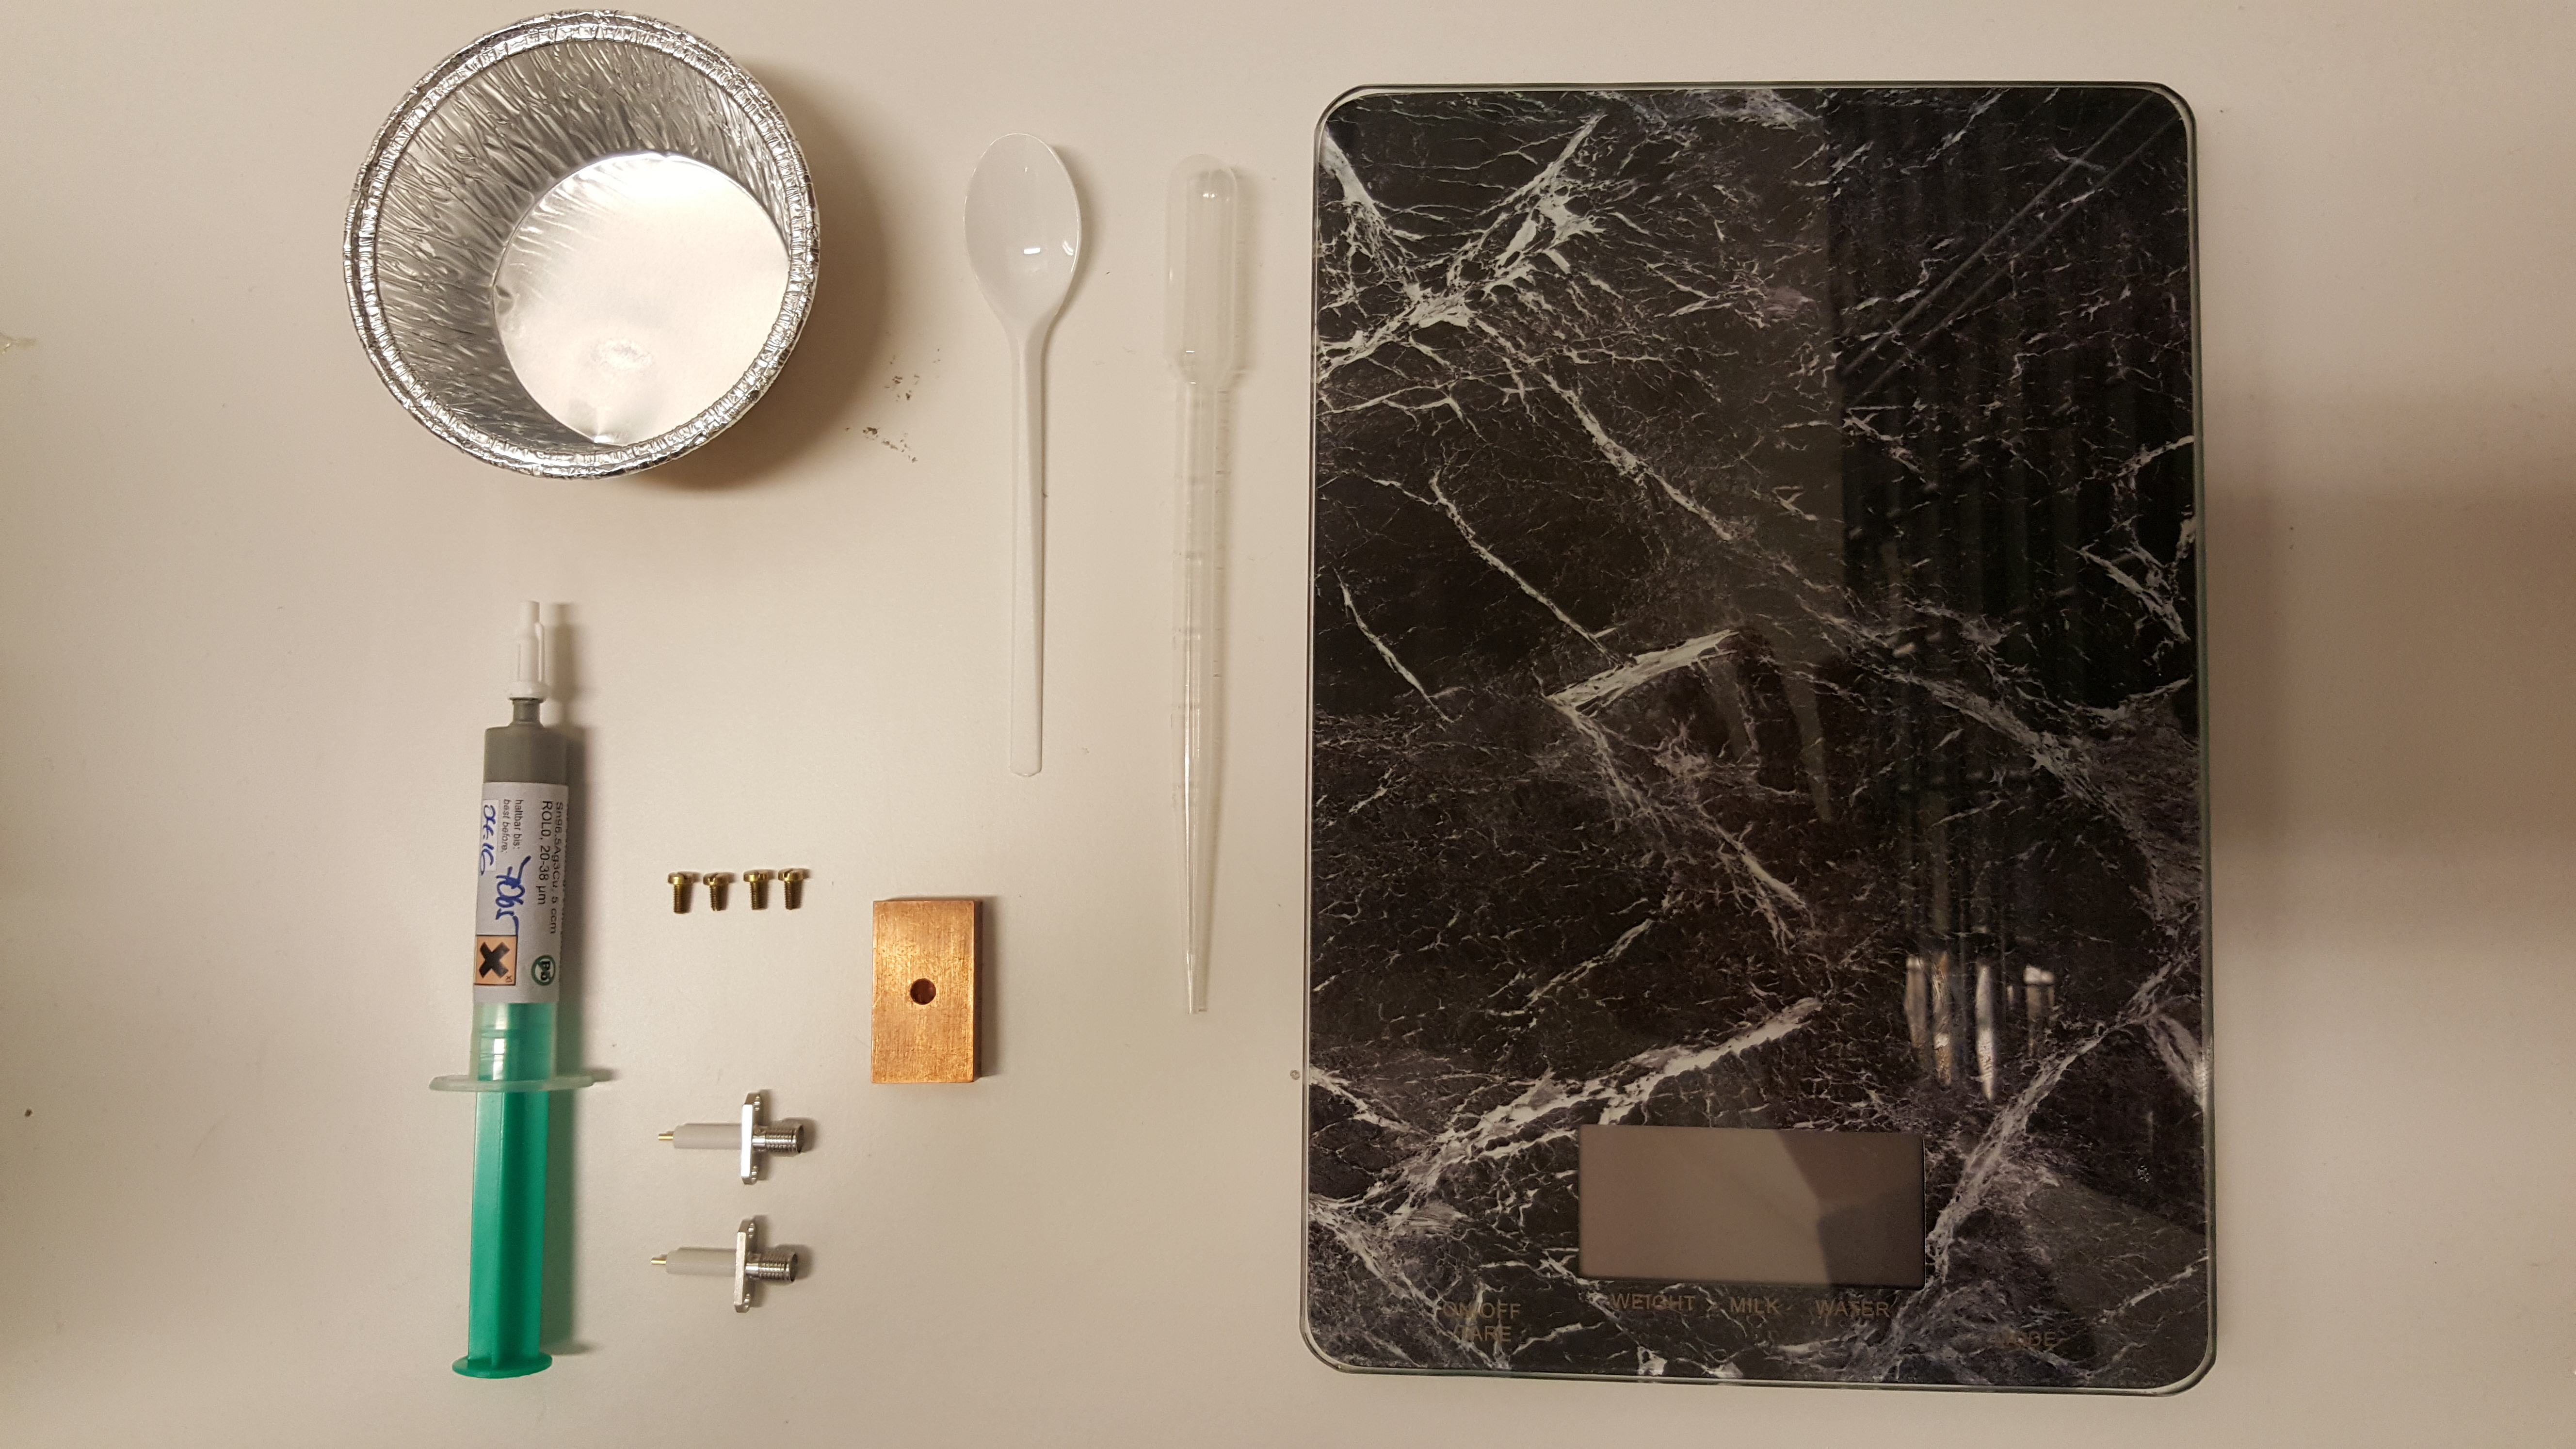
\includegraphics[width=0.65\textwidth]{figure/Filterbilder/filter_material.jpg}};
        \begin{scope}[x={(image.south east)},y={(image.north west)}]
            \node [anchor=west] (form) at (0.1,0.95) {\Large\textbf A};
            \node [anchor=west] (sked) at (0.35,0.935) {\Large\textbf B};
            \node [anchor=west] (pipett) at (0.425,0.925) {\Large\textbf C};
            \node [anchor=west] (paste) at (0.125,0.525) {\Large\textbf D};
            \node [anchor=west] (screws) at (0.255,0.46) {\Large\textbf E};
            \node [anchor=west] (SMA) at (0.315,0.18) {\Large\textbf F};
            \node [anchor=west] (filterbox) at (0.3777,0.32) {\Large\textbf G};
            \node [anchor=west] (scl) at (0.88,0.085) {\Large\textbf H};
        \end{scope}
    \end{tikzpicture}
    \caption{Material som behövs för att göra ett distribuerat lågpassfilter visas i figurer: blandningsform(A), sked(B), pipett(C), lödpasta(D), skruvar(E) för att fästa Radiall R124.464.000W SMA-kontakter(F) i filterlåda av koppar(G) och en våg(H).}
    \label{fig:filter_material}
\end{figure}

%Montering av filter kan delas upp i tre olika steg:


% översikt över det olika stegen borde finnas här ev mer utförligt
%\begin{enumerate}
%    \item Skala SMA kontakter
%    \item Montera och löda SMA kontakter
%    \item Förbereda Stycast och fylla filtret
%\end{enumerate}


Första steget i att göra ett filter är att förbereda SMA kontakterna. Detta innefattar att eventuellt skala av en del av teflonet från kontakten för att få den önskade längden på den frilagda ledaren som sedan ska inkapslas i Stycast. För att få den önskade längden på den frilagda ledaren skars först en bit eltejp till så att bredden på denna motsvarade längden på teflonet som skulle behållas. Eltejpen virades sedan runt SMA kontakten som i \figref{fig:f_SMA_skalning} och det frilagda teflonet skars bort med en hobbykniv. 

%%%%%%%%%%%%%%%%%%%%%%%%%%%%%%%%%%%%%%%%%%%%%%%%%%%%%%%%%
% Bild på SMA kontakt innan, under och efter den skalats
%%%%%%%%%%%%%%%%%%%%%%%%%%%%%%%%%%%%%%%%%%%%%%%%%%%%%%%%%
%0.329
\begin{figure}[h]
    \centering
    \begin{subfigure}{0.25\textwidth}
        \centering
        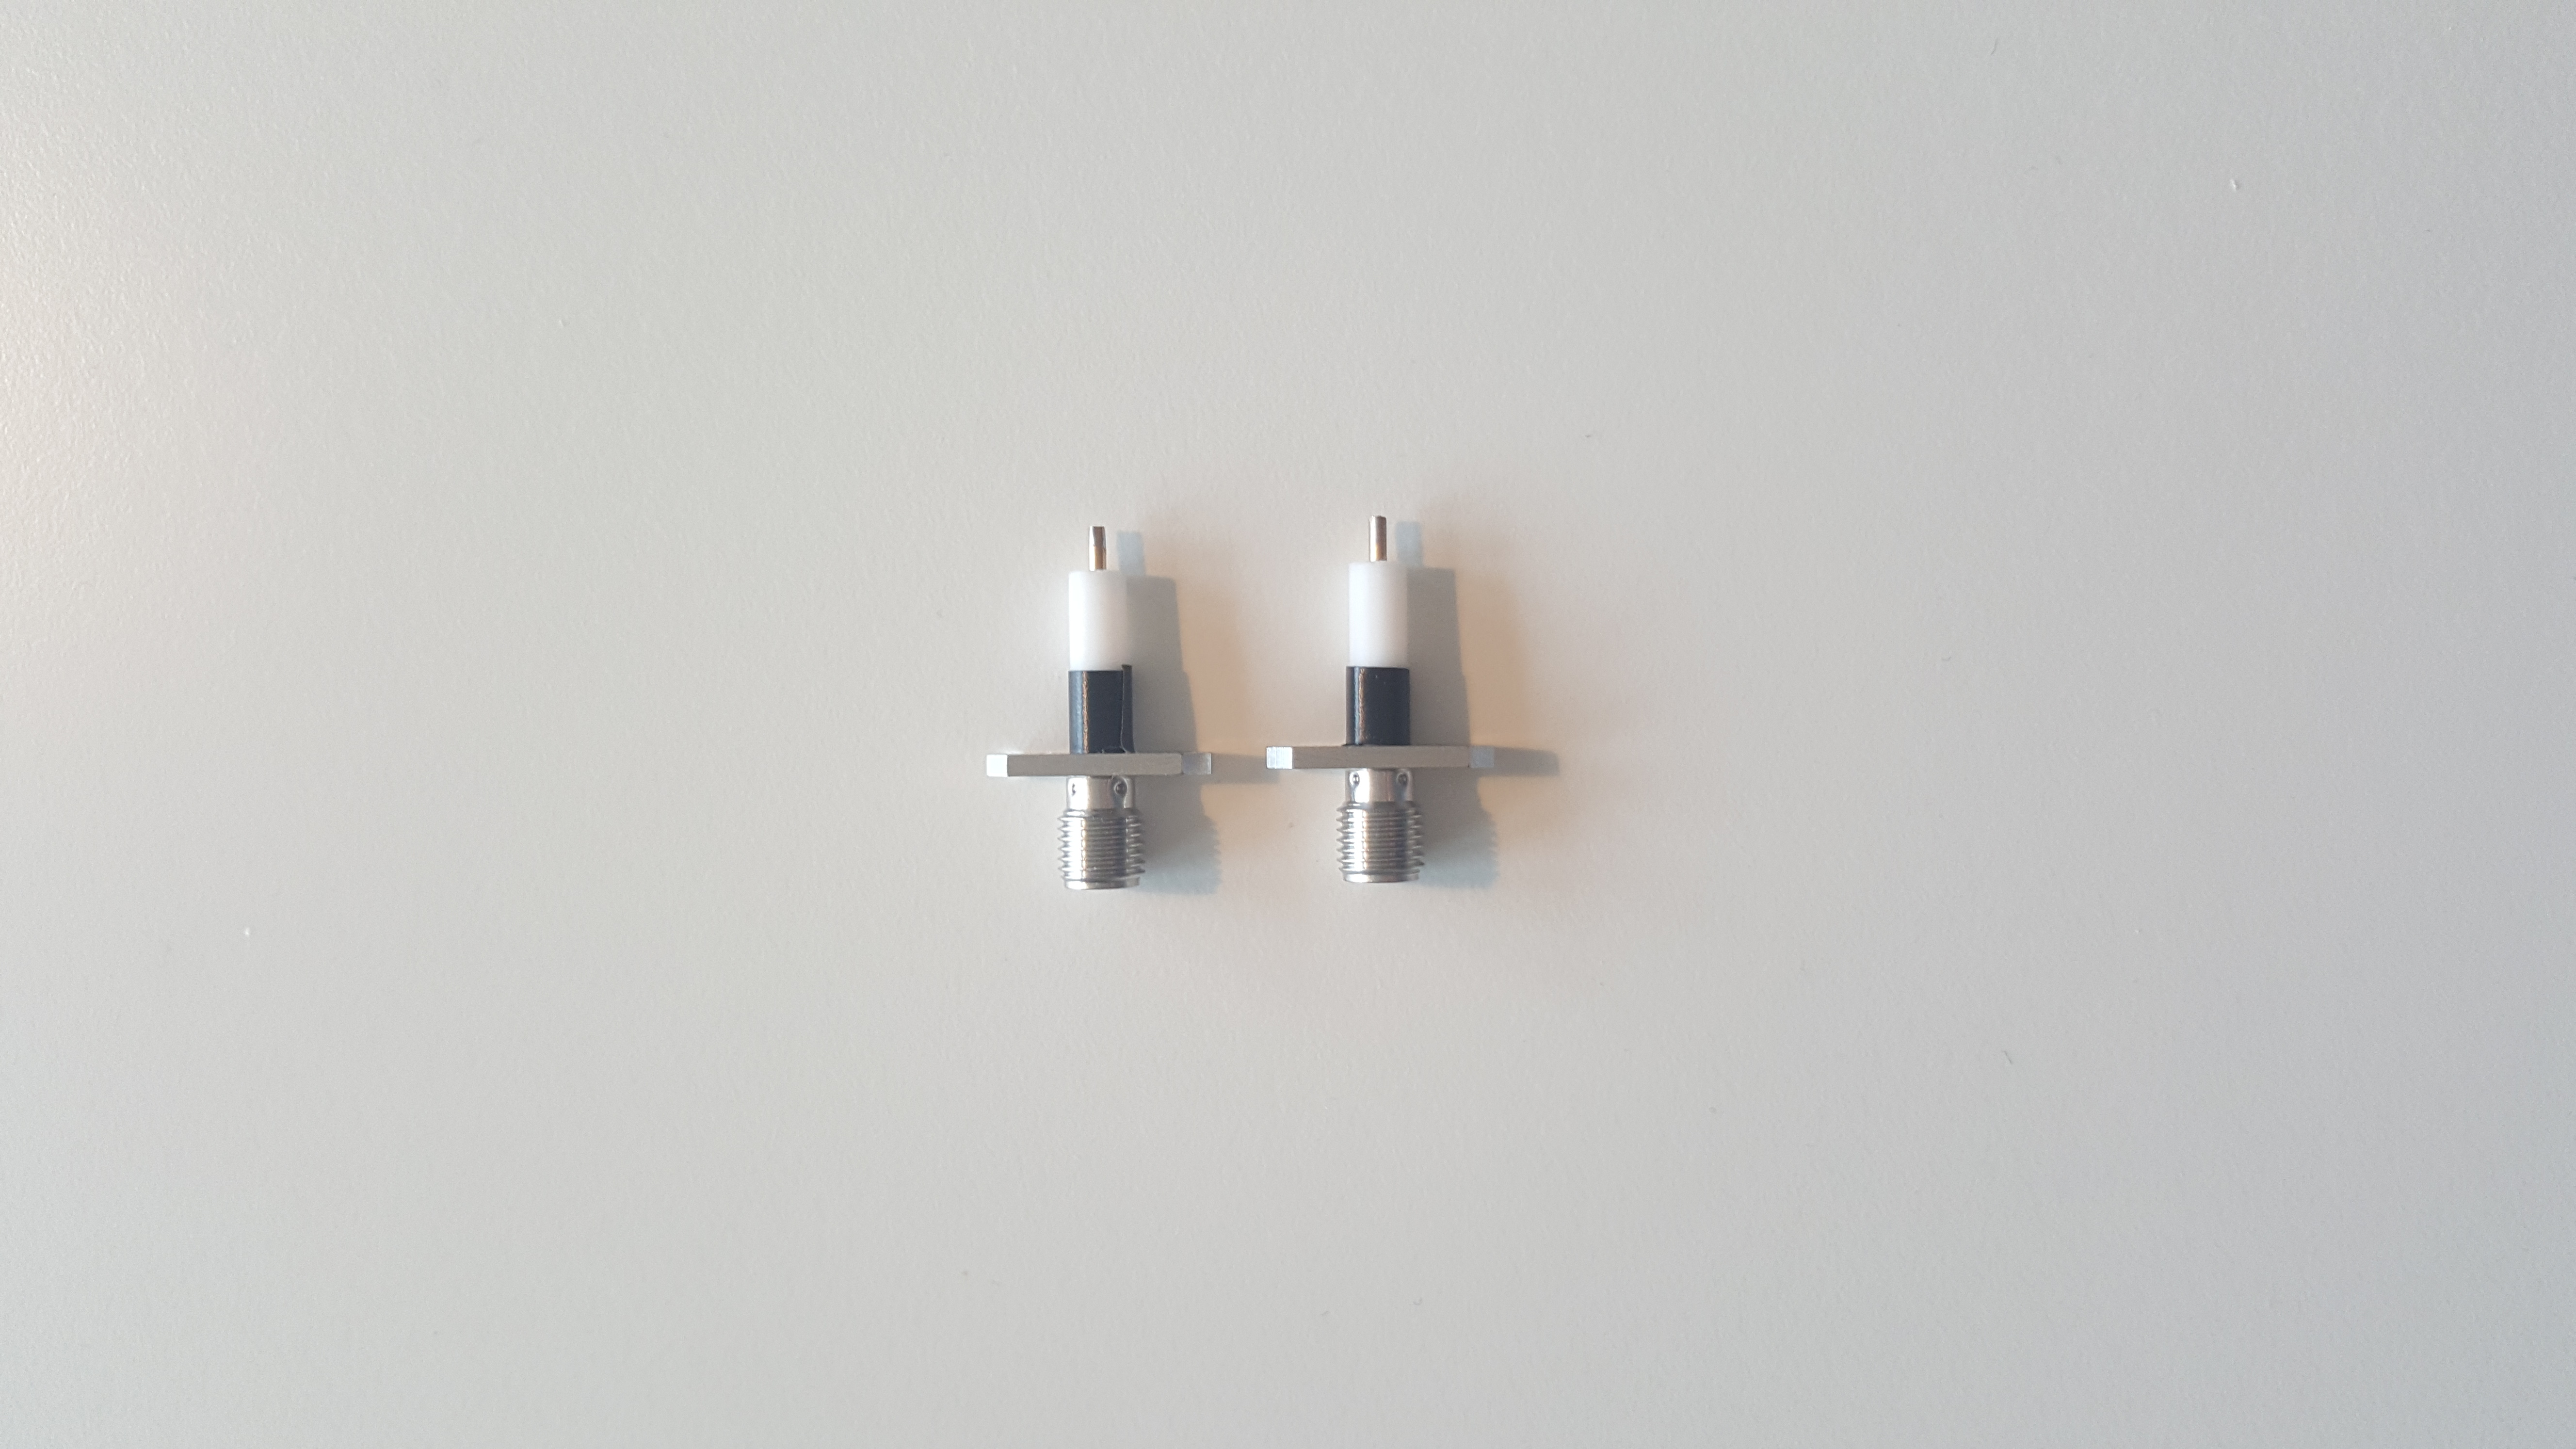
\includegraphics[angle=-90,trim=1450 100 1550 100,clip,width=0.97\linewidth]{figure/Filterbilder/f_sma_skalning.jpg} 
        \caption{}
        \label{fig:f_SMA_skalning}
    \end{subfigure}
        \begin{subfigure}{0.25\textwidth}
        \centering
        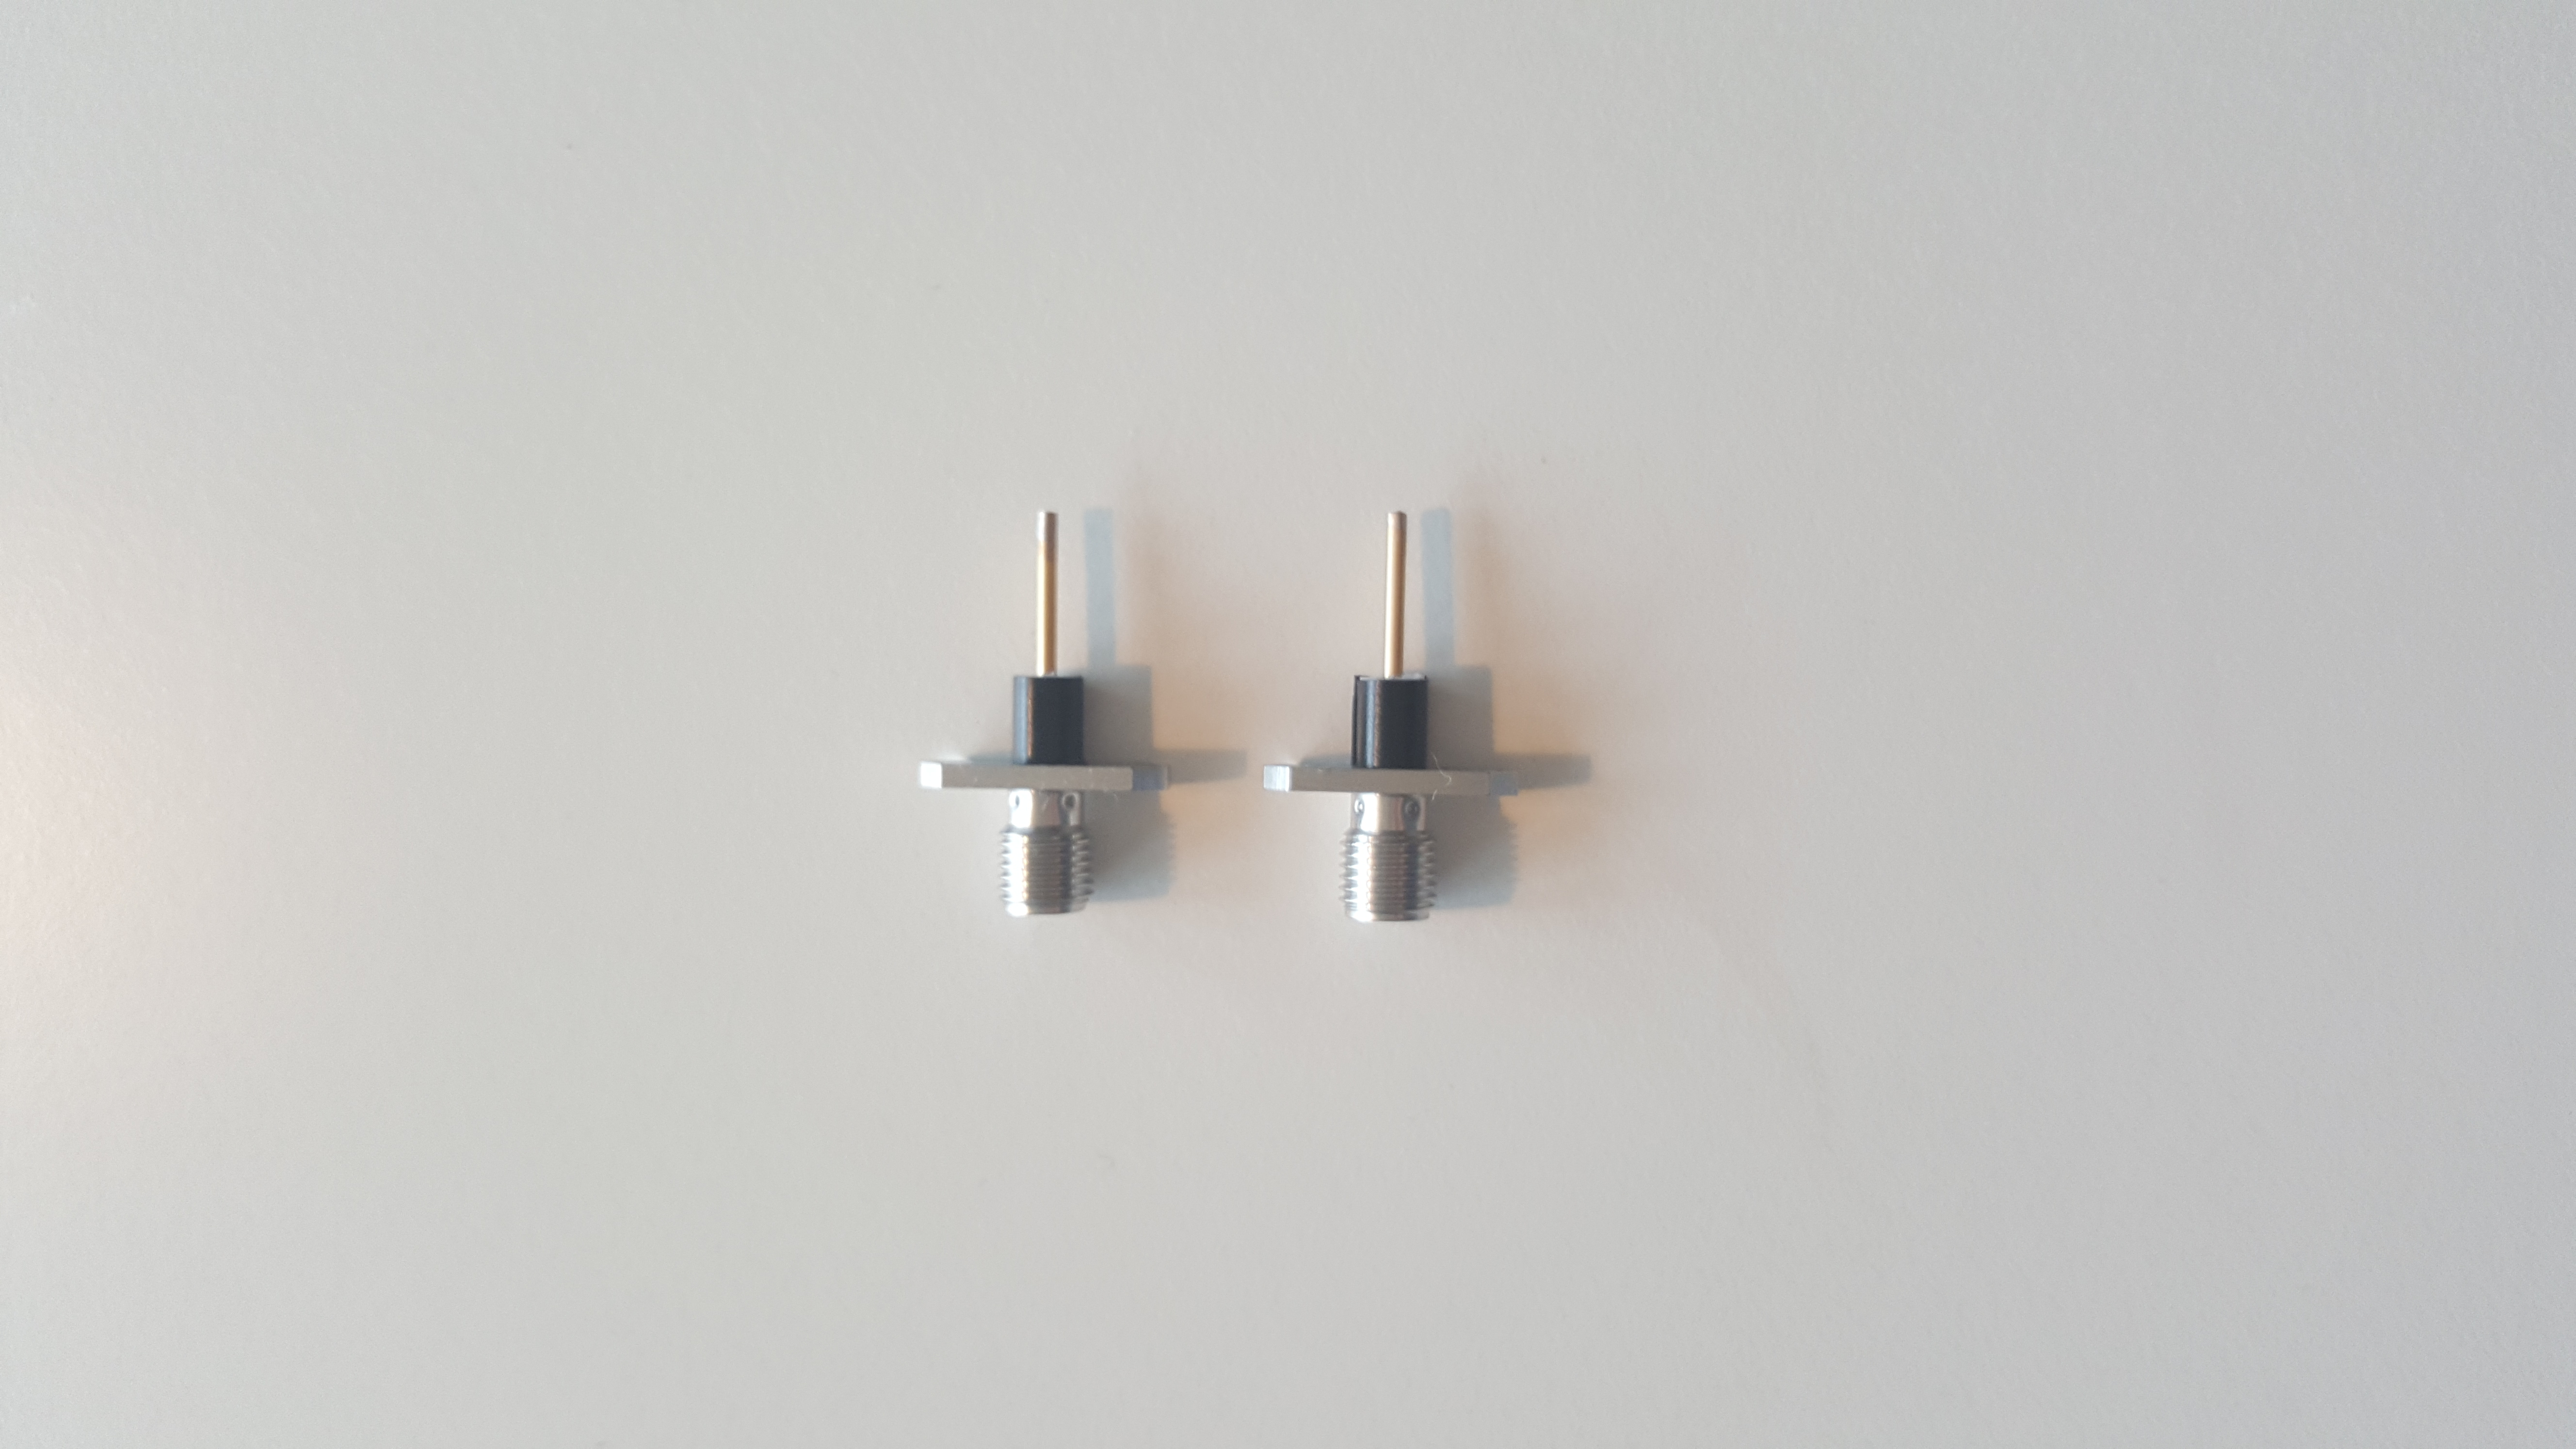
\includegraphics[angle=-90,trim=1450 100 1550 100,clip,width=0.97\linewidth]{figure/Filterbilder/u_sma_skalning.jpg} 
        \caption{}
        \label{fig:u_SMA_skalning}
    \end{subfigure}
        \begin{subfigure}{0.25\textwidth}
        \centering
        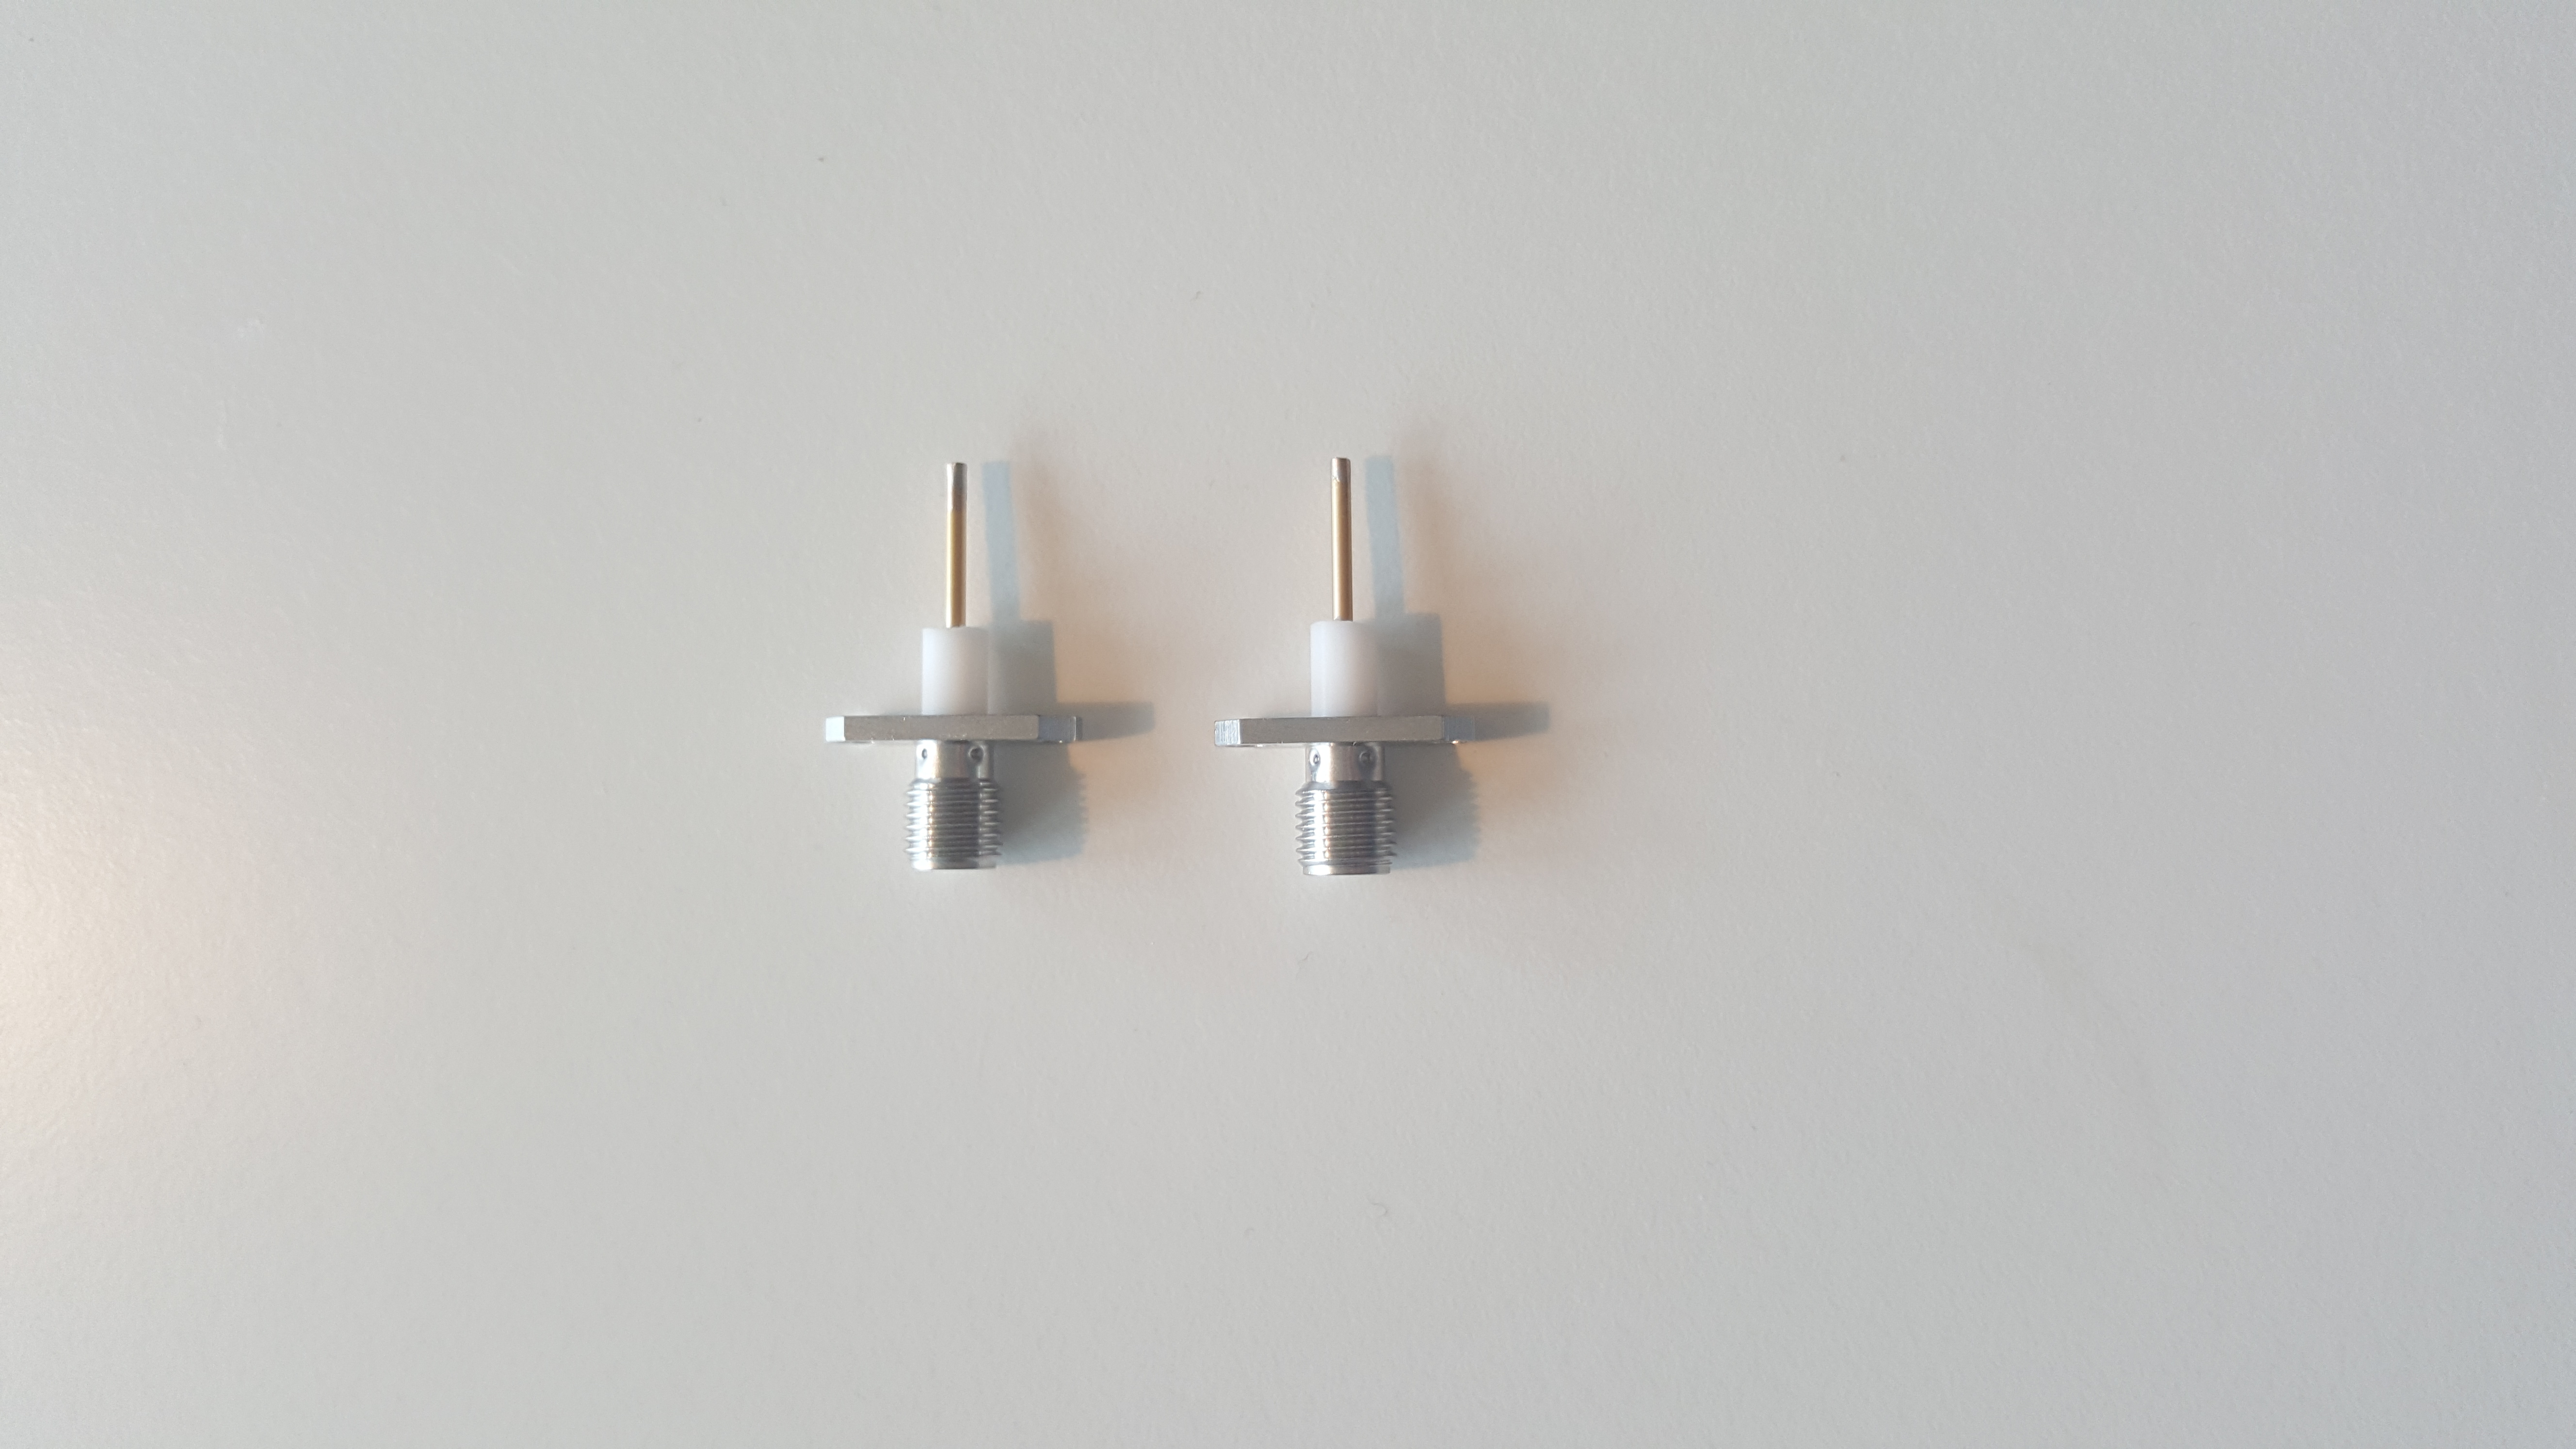
\includegraphics[angle=-90,trim=1300 100 1700 100,clip,width=0.97\linewidth]{figure/Filterbilder/e_sma_skalning.jpg} 
        \caption{}
        \label{fig:e_SMA_skalning}
    \end{subfigure}
    
    
    \caption{Bilden visar de olika stegen i att förbereda SMA-kontakter för att få den önskade längden på den frilagda ledaren. Först virades eltejp runt teflonet som skulle behållas som i \subref{fig:f_SMA_skalning} och därefter skars de frilagda teflonet bort \subref{fig:u_SMA_skalning}. De färdiga SMA-kontakterna visas i \subref{fig:e_SMA_skalning}.}
    \label{fig:SMA_skalning}
\end{figure}

Efter att SMA kontakterna har skalats av till önskad längd så kan dessa monteras i det maskinarbetatade kopparblocket. Först applicerades en liten mängd lödpasta på den ena SMA kontakten som i \figref{fig:prep_SMA} och därefter fördes båda SMA kontakterna in i kopparlådan och skruvades fast. Lödpastan ska omsluta båda ledarna som i \figref{fig:filter_soldering} och de båda ledarna bör vara koaxiala för att minska reflektioner. 

För att löda ihop SMA kontakterna användes en lödkolv med en mejsel-spets för att kunna få bra termisk kontakt mellan de två ledarna och lödpastan. Lödkolven fördes in genom titthålet på kopparlådans översida och placerades mot de två ledarna tills dess att lödpastan smält och flutit ut så att lödningen ser ut som i \figref{fig:post_solder}.

%Därefter kontrollerades lödningens kvalité genom att mäta $S_{21}$-parametern för filtret med VNA i frekvensintervallet \unit[1-50]{GHz}. Magnituden hos $S_{21}$ undersöktes sedan för kraftiga spikar som ett resultat av dåligt matchad impedans, vilket skulle indikera på en dålig lödning. Resultat från dessa mätningar presenteras i \ref{sec:filter_kar}. 

%%%%%%%%%%%%%%%%%%%%%%%%%%%%%%%%%%%%%%%%%%%%%%%%%%%%%%%%%
% Bild på SMA kontakter innan och efter lödning
%%%%%%%%%%%%%%%%%%%%%%%%%%%%%%%%%%%%%%%%%%%%%%%%%%%%%%%%%

\begin{figure}[h]
    \centering
    \begin{subfigure}{0.25\textwidth}
        \centering
        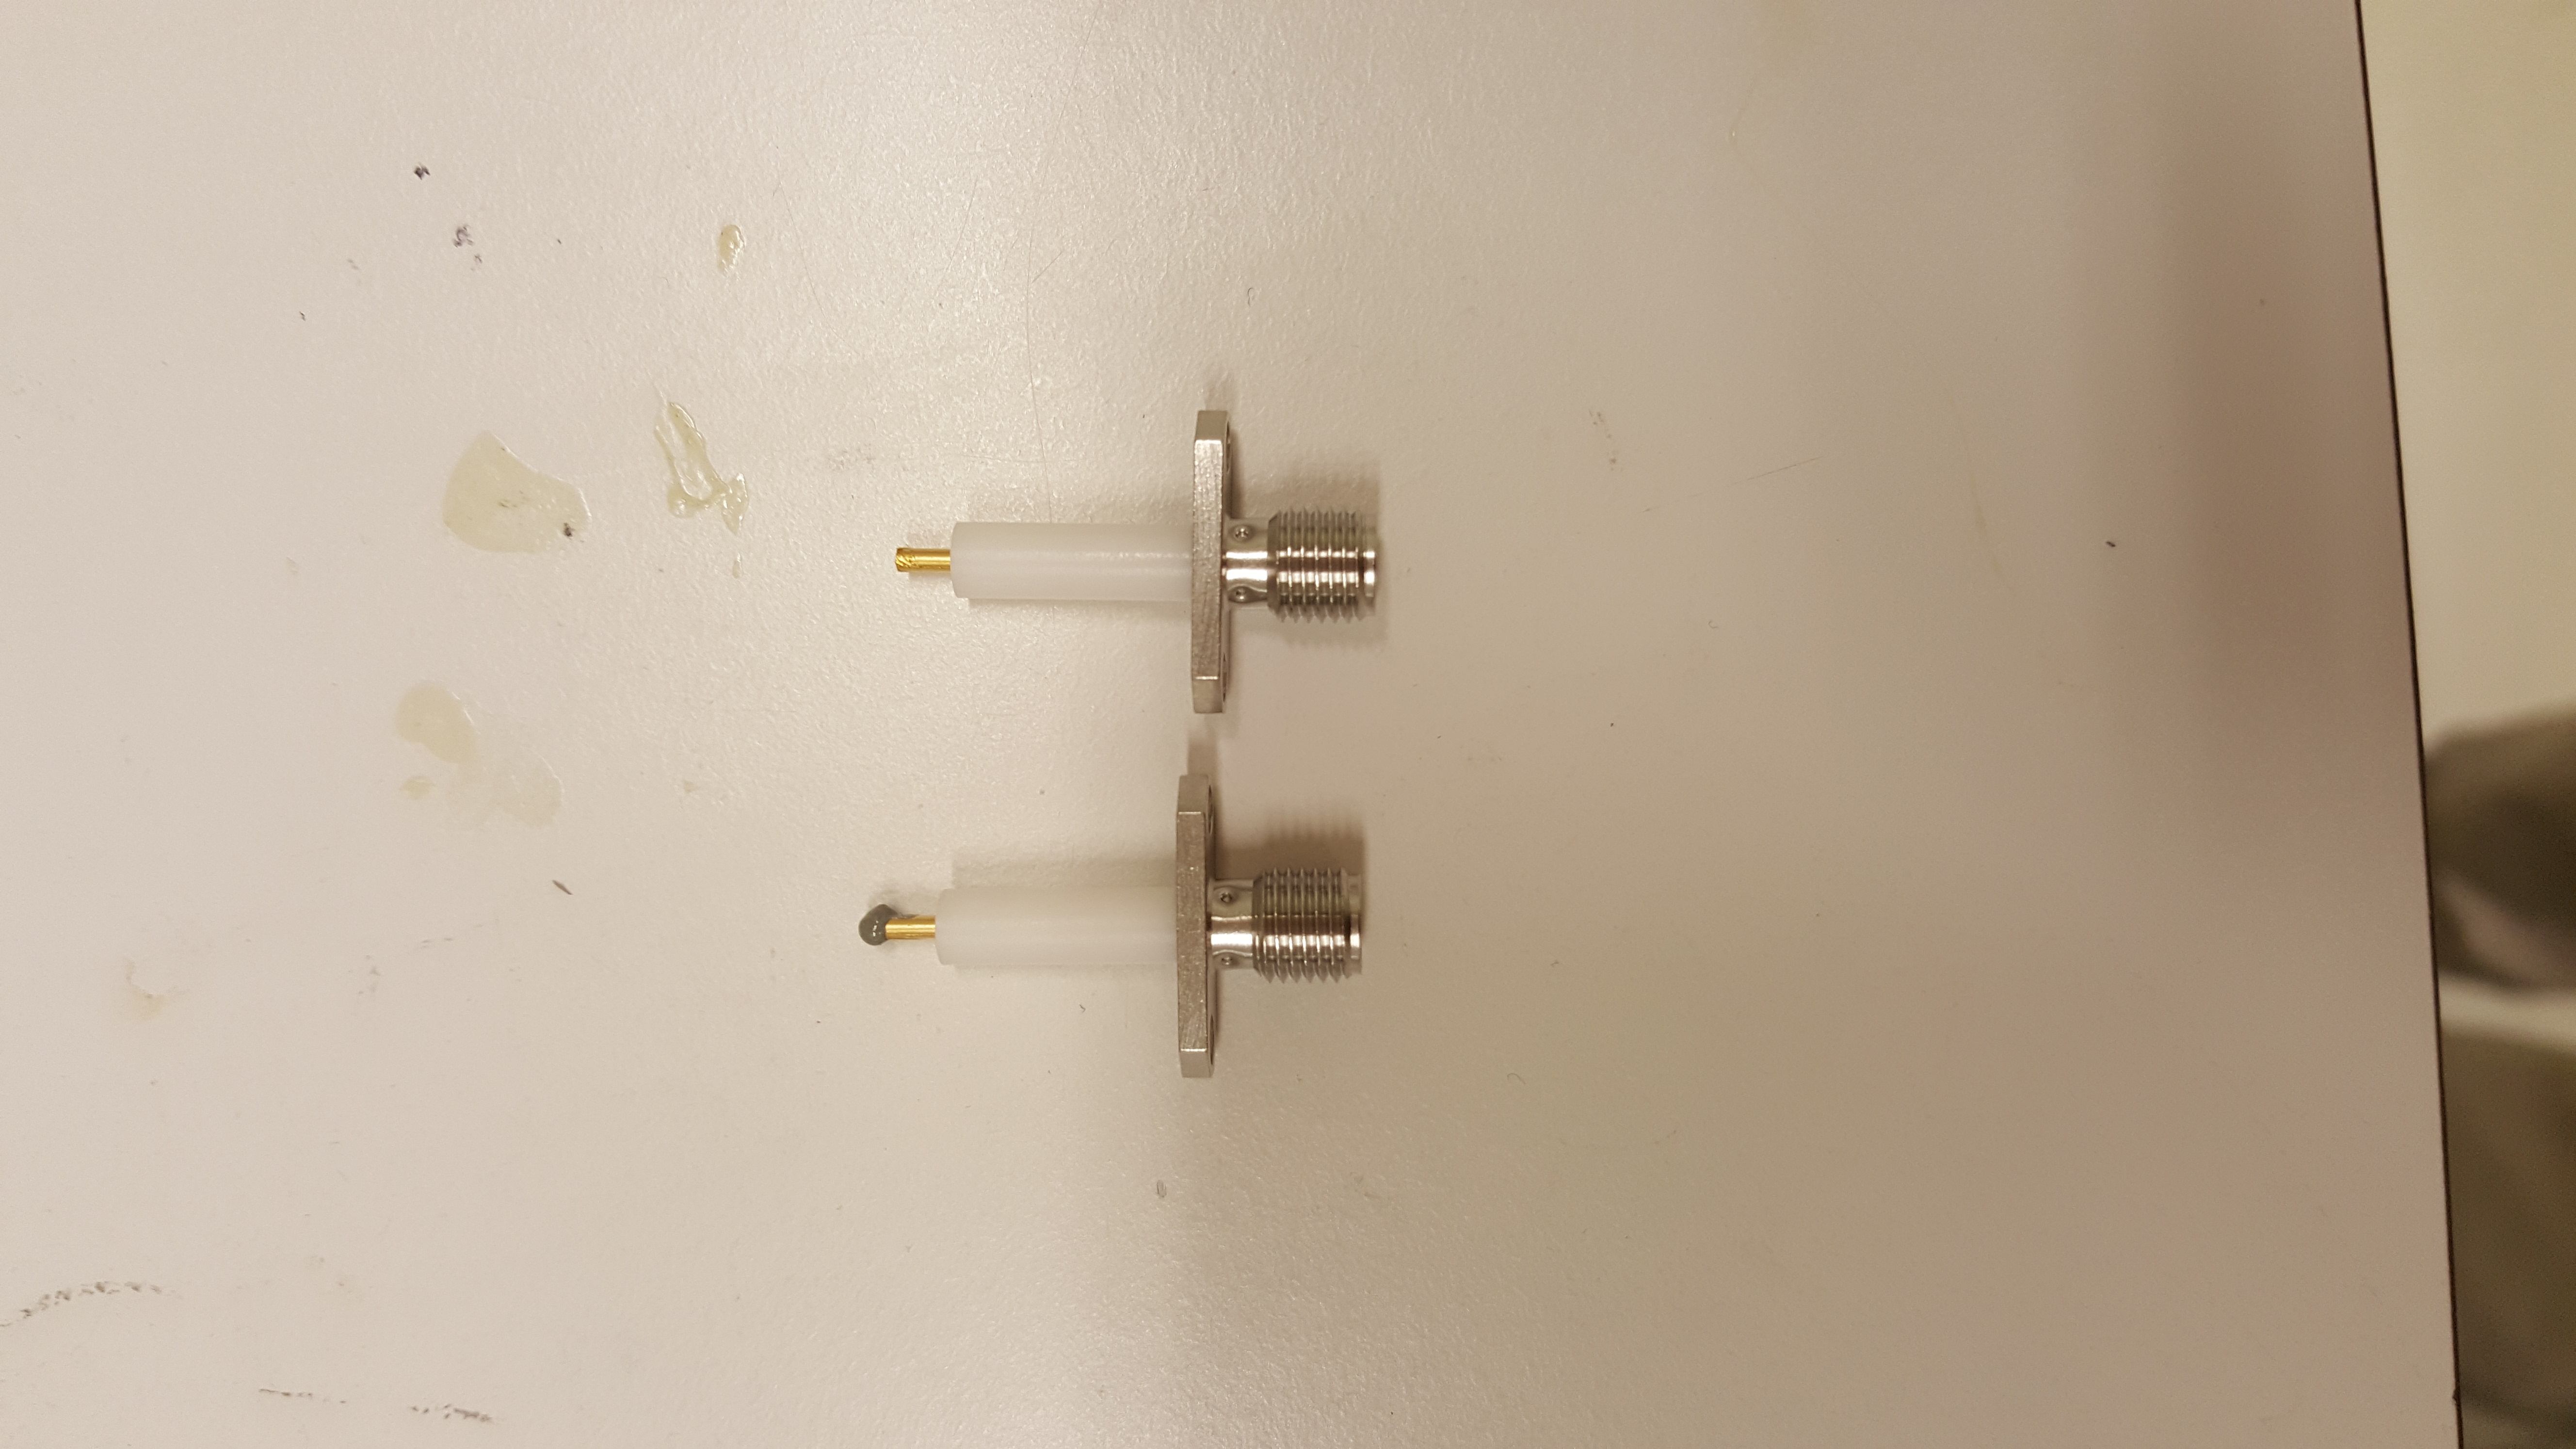
\includegraphics[angle=-90,trim=1200 100 1800 100,clip,width=0.97\linewidth]{figure/Filterbilder/prep_SMA.jpg} 
        \caption{}
        \label{fig:prep_SMA}
    \end{subfigure}
    \begin{subfigure}{0.25\textwidth}
        \centering
        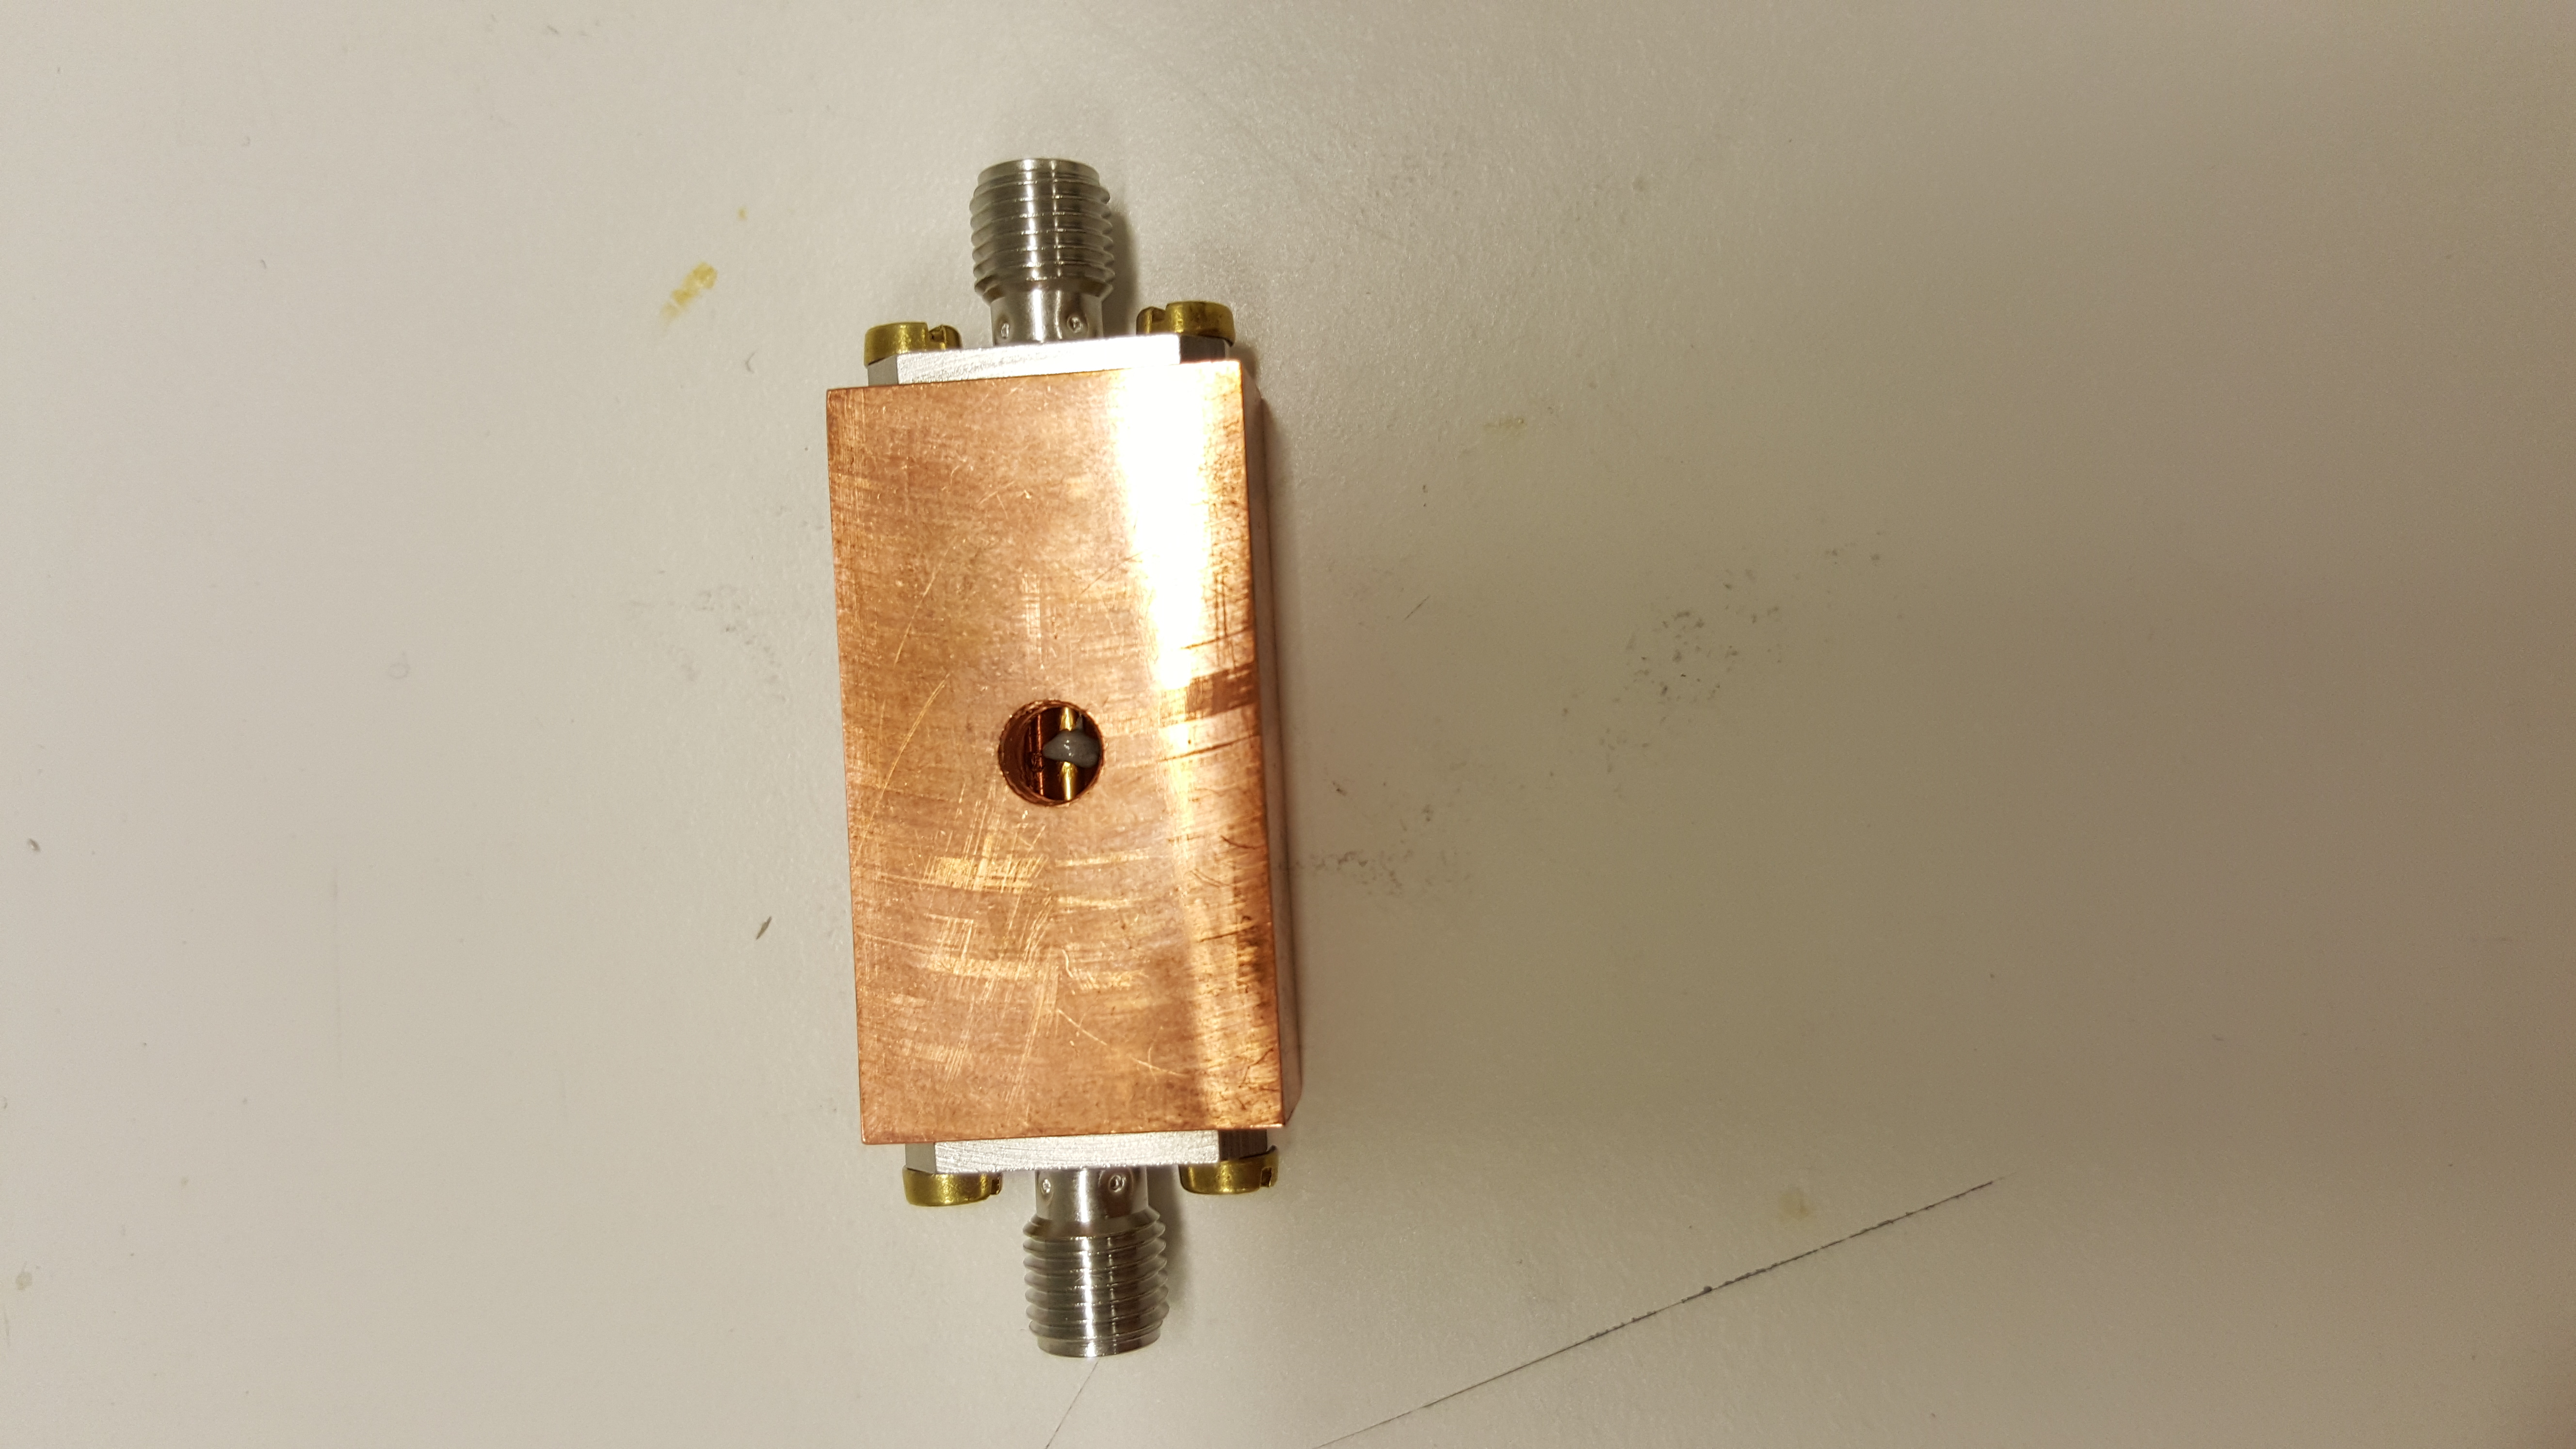
\includegraphics[angle=-90,trim=1000 100 2000 100,clip,width=0.97\linewidth]{figure/Filterbilder/filter_before_solder.jpg} 
        \caption{}
        \label{fig:before_solder}
    \end{subfigure}
    \begin{subfigure}{0.25\textwidth}
        \centering
        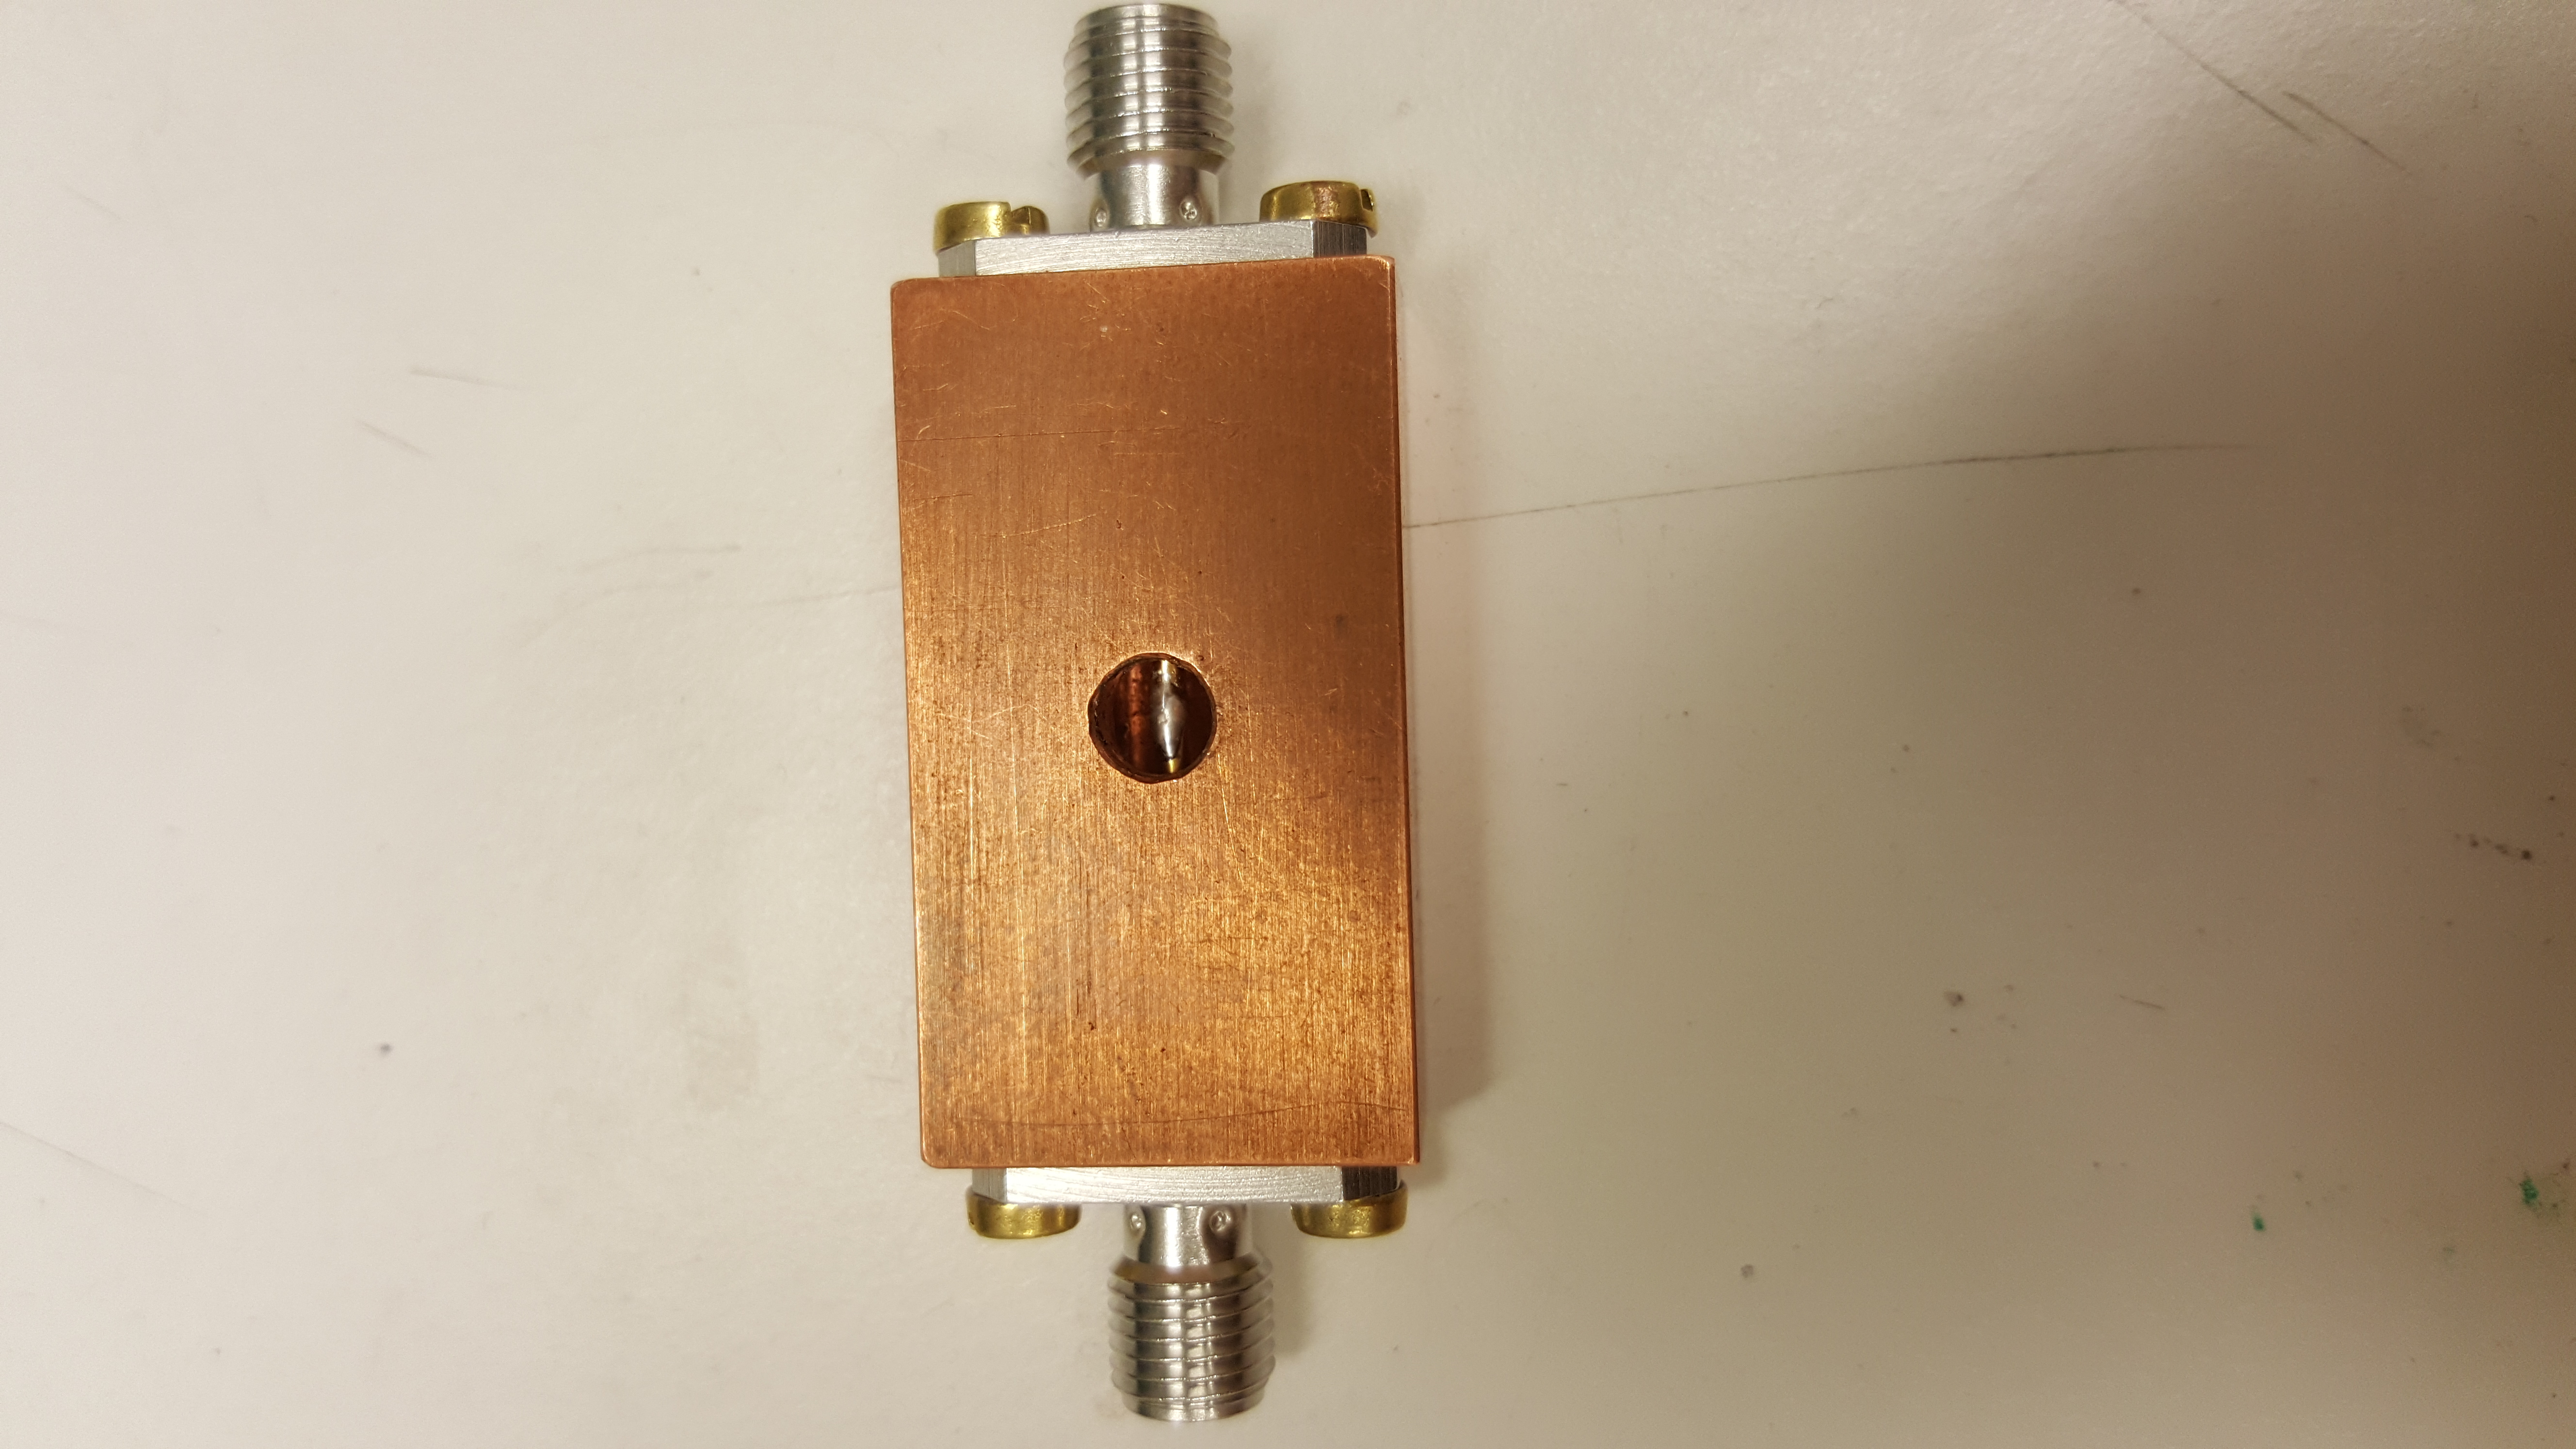
\includegraphics[angle=-90,trim=1200 100 1800 100,clip,width=0.97\linewidth]{figure/Filterbilder/filter_post_solder.jpg} 
        \caption{}
        \label{fig:post_solder}
    \end{subfigure}
    
 \caption{I bilden visas de olika stadierna för att löda ihop ett distribuerat lågpassfilter. I \protect\subref{fig:prep_SMA} har en liten mängd lödpasta applicerats på den vänstra SMA-kontakten. Efter att SMA-kontakterna förts in i koppparlådan så bör lödpastan omsluta båda ledaran som i \subref{fig:before_solder}. I \subref{fig:post_solder} visas den färdiga lödningen.}
 \label{fig:filter_soldering}
\end{figure}


% Måste få in i texten någonstans att förhållandet mellan de olika delarna ska vara A 100:28 B
Efter att lött ihop SMA-kontakterna placerades filtret på en värmeplatta vid \unit[40]{$^\circ$C} för att underlätta när filtret senare ska fyllas med Stycast genom att sänka dess viskositet. Därefter blandades \unit[12,8]{g} Stycast genom att först väga upp \unit[10]{g} Stycast del A och \unit[2,8]{g} Stycast del B och sedan blanda ihop dessa till en homogen vätska i en metallform med hjälp av en plastsked. 

\begin{wrapfigure}{r}{0.25\textwidth}
    \centering
    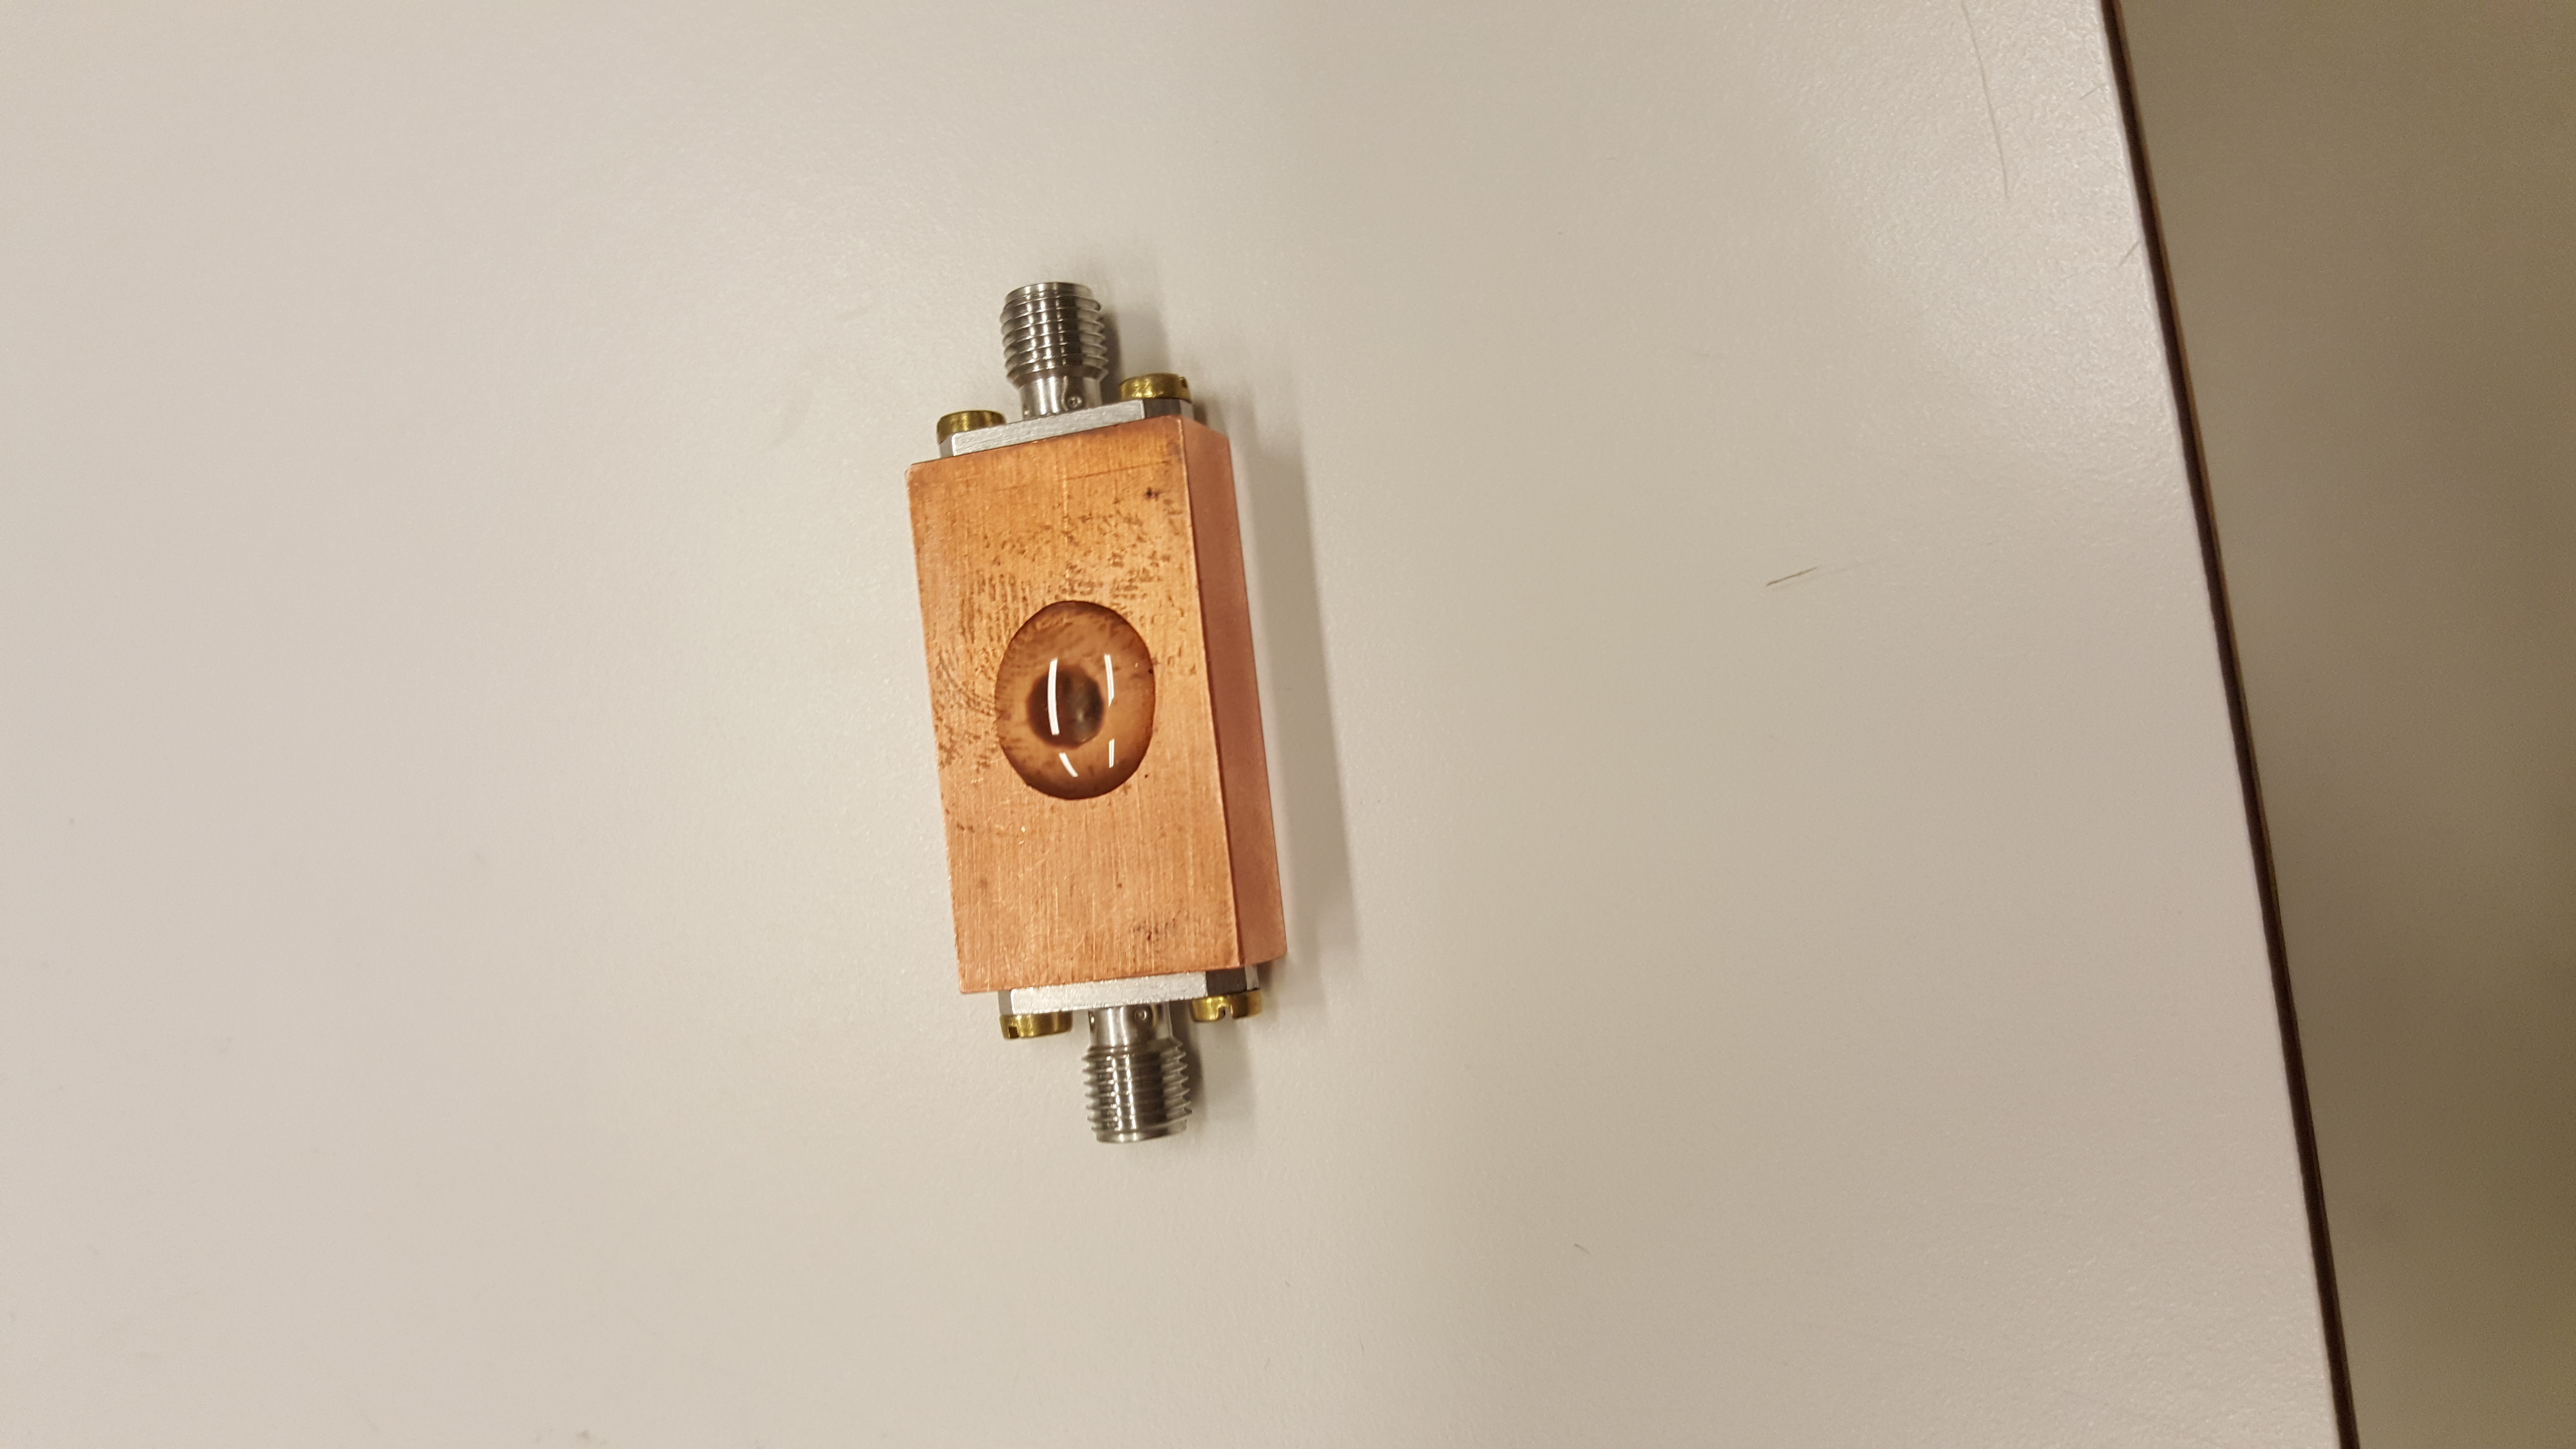
\includegraphics[angle=-90,trim=1250 200 1950 200,clip,width=0.975\linewidth]{figure/Filterbilder/stycast_fill.jpg}
    \caption{Filter som fyllts med Stycast med en stor droppe stycast över titthålet.}
    \label{fig:stycast_filled}
\end{wrapfigure}

Till ett filter går det åt ungefär \unit[$\approx 2$]{g} Stycast beroende på hur lång ledaren som ska kapslas in är. Det är dock nödvändigt att blanda åtminstone \unit[10]{g} för att försäkra sig om att att blandningen är homogen och att förhållandet mellan del A och del B är korrekt. 

Filtret fylldes sedan försiktigt med Stycast med hjälp av en pipett. Pipetten placerades mot kanten av titthålet och Stycast pressades ut långsamt för att förhindra att en bubbla över titthålet bildades, vilket skulle hindra luften i filtret från att kunna komma ut. 

Efter att filtret var fullt placerades en stor droppe Stycast över titthålet som i \figref{fig:stycast_filled} så att ifall det fortfarande fanns lite luft kvar i filtret så skulle detta kunna komma ut och den extra Stycasten som placerades över titthålet skulle kunna fylla igen hålrummet. Filtret härdades sedan vid rumstemperatur i minst 16 timmar. Efter att filtret härdats kan överflödigt Stycast på filtrets ovansida slipas bort. Detta är dock inte nödvändigt för filtrets funktion.


% Filterkarakteristik hade kunnat skippas om vi verkligen behöver sidor
\section{Filterkarakteristik}
\label{sec:filter_kar}
I detta projekt har vi konstruerat filter av tre olika längder i tre uppsättningar och vi kommer fortsättningsvis hänvisa till dessa enligt tabell \ref{tab:filter_list}.

\begin{table}[h]
    \centering
    \caption{Tabell över de individuella filterlängderna samlade i tre olika kategorier: kort, medel och lång.}
    \label{tab:filter_list}
    \begin{tabular}{llll}\toprule
        Namn & \multicolumn{3}{c}{Filterlängd (\unit{cm})} \\
        \midrule
        Kort & 1,895 & 1,88 & 1,825 \\
        Medel & 2,52 & 2,48 & 2,47 \\
        Lång & 3,145 & 3,155 & 3,15\\
        \bottomrule
    \end{tabular}
\end{table}

För att karakterisera samtliga filter användes en Agilent E8364B VNA. Filter anslöts direkt till VNA:n med två SMA M-M adapter och därefter mättes $S_{21}$ i frekvensintervallet \unit[1-50]{GHz}. Mätningen utfördes även innan filtrerna fylldes med Stycast. En mätning av $S_{21}$ utan filter togs också för att använda som referens. Denna referens motsvarar således kablarnas och adapternas påverkan på $S_{21}$, vilket gör det möjligt att särskilja filtrets dämpning från andra dämpande effekter i uppkopplingen.% som skinneffekt och reflektioner på grund av impedansmissmatcher. 

I \figref{fig:filter_kar} visas den uppmätta $|S_{21}|$ för ett filter, innan och efter det fylldes med Stycast, från varje kategori samt en referens. För resterande filter se appendix \ref{}.

\begin{figure}[H]
    \centerfloat
    \begin{subfigure}[t]{0.329\textwidth}
        \centerfloat
        \setlength\figurewidth{0.8\linewidth}
        \setlength\figureheight{11em}
        % This file was created by matlab2tikz.
%
\definecolor{mycolor1}{rgb}{0.1253 0.3242 0.8303}%
\definecolor{mycolor2}{rgb}{0.9990 0.7653 0.2164}%
\definecolor{mycolor3}{rgb}{0.1801 0.7177 0.6424}%
%
\begin{tikzpicture}[%
trim axis left, trim axis right
]

\begin{axis}[%
width=0.951\figurewidth,
height=\figureheight,
at={(0\figurewidth,0\figureheight)},
scale only axis,
xmin=1,
xmax=50,
xlabel style={font=\color{white!15!black}},
xlabel={Frekvens (GHz)},
ymin=-25,
ymax=0,
ylabel style={font=\color{white!15!black}},
ylabel={$|S_{21}|$ (dB)},
axis background/.style={fill=white},
title style={font=\bfseries},
title={Filterlängd \unit[$L=1,880$]{cm}},
axis x line*=bottom,
axis y line*=left,
xmajorgrids,
ymajorgrids,
legend style={legend cell align=left, align=left, draw=white!15!black, legend pos = south west,font=\footnotesize}
]
\addplot [color=mycolor1]
  table[row sep=crcr]{%
1	-1.16019439697266\\
1.40840148925781	-1.19461059570313\\
1.61260223388672	-1.26175689697266\\
1.81680297851563	-1.43586349487305\\
2.02100372314453	-1.67730331420898\\
2.22520446777344	-1.67519760131836\\
2.42940521240234	-1.59586715698242\\
2.63360595703125	-1.45044326782227\\
2.83780670166016	-1.50747680664063\\
3.24620819091797	-1.6981315612793\\
3.45040893554688	-1.87956237792969\\
3.65460968017578	-1.96959686279297\\
4.06301116943359	-2.18230438232422\\
4.2672119140625	-2.20139312744141\\
4.47141265869141	-2.17385101318359\\
4.67561340332031	-2.23030090332031\\
4.87981414794922	-2.19477844238281\\
5.08401489257813	-2.2531852722168\\
5.28821563720703	-2.19477844238281\\
5.49241638183594	-2.36509323120117\\
5.69661712646484	-2.45693206787109\\
5.90081787109375	-2.53515625\\
6.10501861572266	-2.52776336669922\\
6.30921936035156	-2.57235717773438\\
6.51342010498047	-2.56469345092773\\
6.71762084960938	-2.48252105712891\\
6.92182159423828	-2.59459686279297\\
7.12602233886719	-2.60744476318359\\
7.33022308349609	-2.63764190673828\\
7.534423828125	-2.77420043945313\\
7.73862457275391	-2.93844985961914\\
7.94282531738281	-3.03180313110352\\
8.14702606201172	-2.99552536010742\\
8.35122680664063	-2.92645263671875\\
8.55542755126953	-2.86951446533203\\
8.75962829589844	-2.7518424987793\\
8.96382904052734	-2.94639587402344\\
9.16802978515625	-2.93037033081055\\
9.37223052978516	-3.06134033203125\\
9.57643127441406	-3.07764434814453\\
9.78063201904297	-3.36231231689453\\
9.98483276367188	-3.24049758911133\\
10.1890335083008	-3.35360336303711\\
10.5974349975586	-3.25669097900391\\
10.8016357421875	-3.01827621459961\\
11.0058364868164	-3.15408325195313\\
11.2100372314453	-3.11833572387695\\
11.4142379760742	-3.20932006835938\\
11.6184387207031	-3.2580680847168\\
11.822639465332	-3.62111663818359\\
12.0268363952637	-3.57784271240234\\
12.2310371398926	-3.44704437255859\\
12.4352378845215	-3.5361442565918\\
12.6394386291504	-3.57915878295898\\
12.8436393737793	-3.57215118408203\\
13.0478401184082	-3.51372146606445\\
13.2520408630371	-3.62449264526367\\
13.456241607666	-3.63960266113281\\
13.6604423522949	-3.86077499389648\\
13.8646430969238	-3.77748870849609\\
14.0688438415527	-3.98009490966797\\
14.2730445861816	-3.71788787841797\\
14.4772453308105	-3.81061935424805\\
14.6814460754395	-3.70817947387695\\
14.8856468200684	-3.86275482177734\\
15.0898475646973	-3.7950439453125\\
15.2940483093262	-3.86486434936523\\
15.4982490539551	-4.04817962646484\\
15.702449798584	-3.83832931518555\\
15.9066505432129	-4.06875610351563\\
16.1108512878418	-3.94636535644531\\
16.3150520324707	-4.04380035400391\\
16.5192527770996	-4.00730133056641\\
16.7234535217285	-4.08617782592773\\
16.9276542663574	-4.27875900268555\\
17.1318550109863	-4.11851501464844\\
17.3360557556152	-4.23696136474609\\
17.5402565002441	-4.24455642700195\\
17.744457244873	-4.36252593994141\\
17.948657989502	-4.36782073974609\\
18.1528587341309	-4.12881088256836\\
18.3570594787598	-4.49917221069336\\
18.5612602233887	-4.13749694824219\\
18.7654609680176	-4.3330192565918\\
18.9696617126465	-4.27689361572266\\
19.1738624572754	-4.20198440551758\\
19.3780632019043	-4.46118927001953\\
19.5822639465332	-4.12314987182617\\
19.7864646911621	-4.63055038452148\\
19.990665435791	-4.35165405273438\\
20.1948661804199	-4.41668701171875\\
20.3990669250488	-4.73587036132813\\
20.6032676696777	-4.31370162963867\\
20.8074684143066	-4.49352645874023\\
21.0116691589355	-4.65715408325195\\
21.2158699035645	-4.4566650390625\\
21.4200706481934	-4.77475357055664\\
21.6242713928223	-4.39483642578125\\
21.8284721374512	-4.86891937255859\\
22.0326728820801	-4.68338394165039\\
22.236873626709	-4.63353729248047\\
22.4410743713379	-4.93799209594727\\
22.6452751159668	-4.70658111572266\\
22.8494758605957	-4.67916107177734\\
23.0536766052246	-4.81110382080078\\
23.2578773498535	-4.79087448120117\\
23.4620780944824	-4.80014419555664\\
23.6662788391113	-4.95629119873047\\
23.8704795837402	-4.84208679199219\\
24.0746803283691	-4.92272567749023\\
24.278881072998	-4.59413146972656\\
24.483081817627	-5.05683517456055\\
24.6872825622559	-4.7582893371582\\
24.8914833068848	-4.89748001098633\\
25.0956840515137	-4.7105827331543\\
25.2998847961426	-5.06765365600586\\
25.5040855407715	-4.79595184326172\\
25.7082862854004	-5.00085067749023\\
25.9124870300293	-5.12204742431641\\
26.1166877746582	-5.15449905395508\\
26.3208885192871	-5.17451858520508\\
26.525089263916	-5.27431488037109\\
26.7292900085449	-5.21182250976563\\
26.9334907531738	-5.33689498901367\\
27.1376914978027	-5.2160758972168\\
27.3418922424316	-5.58489608764648\\
27.5460929870605	-5.52700805664063\\
27.7502937316895	-5.23764038085938\\
27.9544944763184	-5.62295913696289\\
28.1586952209473	-5.27834320068359\\
28.3628959655762	-5.46773910522461\\
28.5670967102051	-5.51028442382813\\
28.771297454834	-5.42916488647461\\
28.9754981994629	-5.53417205810547\\
29.1796989440918	-5.41532135009766\\
29.3838996887207	-5.93757247924805\\
29.5881004333496	-5.75418853759766\\
29.7923011779785	-5.66700744628906\\
29.9965019226074	-5.72772216796875\\
30.2007026672363	-5.55557250976563\\
30.4049034118652	-5.64014053344727\\
30.6091041564941	-5.50594711303711\\
30.813304901123	-6.3717155456543\\
31.017505645752	-5.44407272338867\\
31.2217063903809	-6.34483337402344\\
31.4259071350098	-6.21534729003906\\
31.6301040649414	-5.85131072998047\\
31.8343048095703	-5.65256500244141\\
32.0385055541992	-5.75090408325195\\
32.2427062988281	-5.86740493774414\\
32.446907043457	-6.07308959960938\\
32.6511077880859	-5.92707061767578\\
32.8553085327148	-6.68338775634766\\
33.0595092773438	-6.00259399414063\\
33.2637100219727	-6.18016815185547\\
33.4679107666016	-5.89849853515625\\
33.6721115112305	-6.31182861328125\\
33.8763122558594	-6.04426956176758\\
34.0805130004883	-5.99222183227539\\
34.2847137451172	-6.44392395019531\\
34.4889144897461	-6.06501770019531\\
34.693115234375	-6.87575149536133\\
34.8973159790039	-6.3222770690918\\
35.1015167236328	-5.96397018432617\\
35.3057174682617	-6.468505859375\\
35.5099182128906	-5.9174919128418\\
35.7141189575195	-6.65866470336914\\
35.9183197021484	-6.97575759887695\\
36.1225204467773	-5.82676696777344\\
36.3267211914063	-6.23660278320313\\
36.5309219360352	-6.23672103881836\\
36.7351226806641	-6.15848159790039\\
36.939323425293	-6.89974594116211\\
37.1435241699219	-6.39983367919922\\
37.3477249145508	-6.46829986572266\\
37.5519256591797	-6.65950393676758\\
37.7561264038086	-6.37036895751953\\
37.9603271484375	-6.45318222045898\\
38.1645278930664	-6.84955978393555\\
38.3687286376953	-6.79656219482422\\
38.5729293823242	-6.76377487182617\\
38.7771301269531	-6.69974136352539\\
38.981330871582	-7.21593856811523\\
39.1855316162109	-7.44292449951172\\
39.3897323608398	-6.81509399414063\\
39.5939331054688	-7.26265716552734\\
39.7981338500977	-7.48611450195313\\
40.0023345947266	-7.83878707885742\\
40.2065353393555	-7.60520553588867\\
40.4107360839844	-8.29539108276367\\
40.6149368286133	-8.45922470092773\\
40.8191375732422	-8.95351028442383\\
41.0233383178711	-9.10346603393555\\
41.2275390625	-9.15691375732422\\
41.4317398071289	-9.26258087158203\\
41.6359405517578	-8.60441207885742\\
41.8401412963867	-7.84791946411133\\
42.0443420410156	-7.73397827148438\\
42.2485427856445	-6.85037612915039\\
42.4527435302734	-7.39094543457031\\
42.6569442749023	-7.8229866027832\\
42.8611450195313	-10.7145843505859\\
43.0653457641602	-8.63249588012695\\
43.2695465087891	-7.4626350402832\\
43.473747253418	-6.8858528137207\\
43.6779479980469	-6.91415405273438\\
43.8821487426758	-6.9224967956543\\
44.0863494873047	-6.77080917358398\\
44.2905502319336	-6.37398147583008\\
44.4947509765625	-6.85309219360352\\
44.6989517211914	-6.63526153564453\\
44.903148651123	-6.26382446289063\\
45.107349395752	-7.07452392578125\\
45.3115501403809	-6.15454483032227\\
45.5157508850098	-6.98114776611328\\
45.7199516296387	-6.99844360351563\\
45.9241523742676	-7.47502136230469\\
46.1283531188965	-8.60497665405273\\
46.3325538635254	-8.58415603637695\\
46.5367546081543	-13.2958793640137\\
46.7409553527832	-13.1753807067871\\
46.9451560974121	-8.635498046875\\
47.149356842041	-8.10023880004883\\
47.3535575866699	-7.92776107788086\\
47.5577583312988	-7.11529541015625\\
47.7619590759277	-8.85005187988281\\
47.9661598205566	-7.60174560546875\\
48.1703605651855	-7.63908386230469\\
48.3745613098145	-8.4350700378418\\
48.5787620544434	-8.99440383911133\\
48.7829627990723	-9.45951843261719\\
48.9871635437012	-11.8883895874023\\
49.1913642883301	-18.3638687133789\\
49.395565032959	-10.720142364502\\
49.5997657775879	-8.44327926635742\\
49.8039665222168	-6.95102310180664\\
};
\addlegendentry{Referens}

\addplot [color=mycolor2]
  table[row sep=crcr]{%
1	-1.29994201660156\\
1.20420074462891	-1.3363151550293\\
1.40840148925781	-1.48907852172852\\
1.61260223388672	-1.5771598815918\\
2.02100372314453	-2.06618118286133\\
2.22520446777344	-2.13954162597656\\
2.42940521240234	-2.081787109375\\
2.63360595703125	-1.72855758666992\\
2.83780670166016	-1.98135757446289\\
3.04200744628906	-1.92000579833984\\
3.24620819091797	-2.24037170410156\\
3.45040893554688	-2.11968994140625\\
3.65460968017578	-2.46351623535156\\
3.85881042480469	-2.54692077636719\\
4.06301116943359	-2.76802825927734\\
4.2672119140625	-2.85041427612305\\
4.47141265869141	-2.63742446899414\\
4.67561340332031	-2.81665802001953\\
4.87981414794922	-2.632568359375\\
5.08401489257813	-2.79999542236328\\
5.28821563720703	-2.68349456787109\\
5.49241638183594	-2.69384765625\\
5.69661712646484	-2.80041885375977\\
5.90081787109375	-2.69147491455078\\
6.10501861572266	-2.79545974731445\\
6.30921936035156	-2.66600036621094\\
6.51342010498047	-2.79165267944336\\
6.71762084960938	-2.59981155395508\\
6.92182159423828	-2.70987319946289\\
7.12602233886719	-2.74362182617188\\
7.33022308349609	-2.75095748901367\\
7.534423828125	-2.96223068237305\\
7.94282531738281	-3.26189422607422\\
8.14702606201172	-3.14957809448242\\
8.35122680664063	-3.11167144775391\\
8.55542755126953	-3.06393051147461\\
8.75962829589844	-2.98831176757813\\
8.96382904052734	-3.15640640258789\\
9.16802978515625	-3.13209533691406\\
9.37223052978516	-3.19215774536133\\
9.78063201904297	-3.49595642089844\\
9.98483276367188	-3.52981948852539\\
10.1890335083008	-3.50339508056641\\
10.3932342529297	-3.57731246948242\\
10.5974349975586	-3.49699401855469\\
10.8016357421875	-3.362060546875\\
11.0058364868164	-3.74913787841797\\
11.2100372314453	-3.54514312744141\\
11.4142379760742	-4.0376091003418\\
11.6184387207031	-3.91347503662109\\
11.822639465332	-4.64686965942383\\
12.0268363952637	-4.13230514526367\\
12.2310371398926	-4.37051391601563\\
12.4352378845215	-4.19669342041016\\
12.6394386291504	-4.72164535522461\\
12.8436393737793	-4.7106819152832\\
13.0478401184082	-4.58013916015625\\
13.2520408630371	-5.1107177734375\\
13.456241607666	-4.81185150146484\\
13.6604423522949	-5.2047119140625\\
13.8646430969238	-5.17806625366211\\
14.0688438415527	-4.81884765625\\
14.2730445861816	-4.54765319824219\\
14.4772453308105	-4.21148681640625\\
14.6814460754395	-4.1467399597168\\
14.8856468200684	-4.01105499267578\\
15.0898475646973	-3.99749374389648\\
15.2940483093262	-4.18499374389648\\
15.4982490539551	-4.25644302368164\\
15.702449798584	-4.1214714050293\\
15.9066505432129	-4.31855392456055\\
16.1108512878418	-4.10322570800781\\
16.3150520324707	-4.29716110229492\\
16.5192527770996	-4.27089309692383\\
16.9276542663574	-4.42748641967773\\
17.1318550109863	-4.37494659423828\\
17.3360557556152	-4.51415252685547\\
17.5402565002441	-4.50011444091797\\
17.744457244873	-4.63975524902344\\
17.948657989502	-4.55938720703125\\
18.1528587341309	-4.40222549438477\\
18.3570594787598	-4.68772506713867\\
18.5612602233887	-4.43343734741211\\
18.9696617126465	-4.69423294067383\\
19.1738624572754	-4.47960662841797\\
19.3780632019043	-4.91791534423828\\
19.990665435791	-5.37523651123047\\
20.1948661804199	-5.0899658203125\\
20.3990669250488	-6.363525390625\\
20.6032676696777	-5.69406890869141\\
20.8074684143066	-6.06443023681641\\
21.0116691589355	-6.12159729003906\\
21.2158699035645	-6.37014007568359\\
21.4200706481934	-6.12430953979492\\
21.6242713928223	-4.97276306152344\\
21.8284721374512	-5.38557434082031\\
22.0326728820801	-4.90323257446289\\
22.236873626709	-4.84232711791992\\
22.4410743713379	-5.23464584350586\\
22.6452751159668	-4.9289665222168\\
22.8494758605957	-4.91756439208984\\
23.0536766052246	-5.15066528320313\\
23.2578773498535	-5.06739044189453\\
23.4620780944824	-5.12820053100586\\
23.6662788391113	-5.10380935668945\\
23.8704795837402	-5.3281135559082\\
24.0746803283691	-5.58065795898438\\
24.278881072998	-5.66831207275391\\
24.483081817627	-6.07363510131836\\
24.6872825622559	-5.5916748046875\\
24.8914833068848	-5.8671989440918\\
25.0956840515137	-5.2945442199707\\
25.2998847961426	-5.97107696533203\\
25.5040855407715	-5.36094284057617\\
25.7082862854004	-5.78896331787109\\
25.9124870300293	-5.66799926757813\\
26.3208885192871	-5.48585510253906\\
26.525089263916	-5.53875732421875\\
26.7292900085449	-5.41798782348633\\
26.9334907531738	-5.74960327148438\\
27.1376914978027	-5.53708267211914\\
27.3418922424316	-5.86014175415039\\
27.5460929870605	-5.81472778320313\\
27.7502937316895	-5.71480941772461\\
27.9544944763184	-6.05071640014648\\
28.1586952209473	-6.69342803955078\\
28.3628959655762	-7.28529357910156\\
28.5670967102051	-7.3287467956543\\
28.771297454834	-6.86140823364258\\
28.9754981994629	-7.2075309753418\\
29.1796989440918	-6.217529296875\\
29.3838996887207	-6.77443695068359\\
29.5881004333496	-6.65105438232422\\
29.7923011779785	-6.65536117553711\\
29.9965019226074	-7.00601196289063\\
30.2007026672363	-6.68882369995117\\
30.4049034118652	-6.9456672668457\\
30.6091041564941	-6.5401725769043\\
30.813304901123	-7.73144912719727\\
31.017505645752	-6.76728439331055\\
31.2217063903809	-7.60752868652344\\
31.4259071350098	-6.50616455078125\\
31.6301040649414	-6.50608825683594\\
31.8343048095703	-6.26707458496094\\
32.0385055541992	-6.21114349365234\\
32.2427062988281	-6.517578125\\
32.446907043457	-6.76035308837891\\
32.6511077880859	-6.25339889526367\\
32.8553085327148	-6.63531112670898\\
33.0595092773438	-6.01899337768555\\
33.2637100219727	-6.59830474853516\\
33.4679107666016	-7.25023651123047\\
33.6721115112305	-8.30074310302734\\
33.8763122558594	-8.7348518371582\\
34.0805130004883	-8.78713607788086\\
34.2847137451172	-10.7541465759277\\
34.4889144897461	-10.4243469238281\\
34.693115234375	-11.4430046081543\\
34.8973159790039	-9.7071533203125\\
35.1015167236328	-8.9893684387207\\
35.3057174682617	-8.87477493286133\\
35.5099182128906	-7.74598693847656\\
35.7141189575195	-7.36741256713867\\
35.9183197021484	-7.62796401977539\\
36.1225204467773	-7.00324249267578\\
36.3267211914063	-7.57351303100586\\
36.5309219360352	-7.67173767089844\\
36.7351226806641	-6.71393203735352\\
36.939323425293	-7.35406875610352\\
37.1435241699219	-7.30956649780273\\
37.3477249145508	-7.98071670532227\\
37.5519256591797	-9.33837127685547\\
37.7561264038086	-9.35687255859375\\
37.9603271484375	-10.5710029602051\\
38.1645278930664	-11.8548622131348\\
38.3687286376953	-10.5751037597656\\
38.5729293823242	-10.709529876709\\
38.7771301269531	-10.6984748840332\\
38.981330871582	-10.2567138671875\\
39.1855316162109	-8.98644256591797\\
39.3897323608398	-8.01835250854492\\
39.5939331054688	-8.09015274047852\\
39.7981338500977	-8.91913986206055\\
40.2065353393555	-9.95008850097656\\
40.4107360839844	-10.115608215332\\
40.6149368286133	-11.4627685546875\\
40.8191375732422	-11.1868515014648\\
41.0233383178711	-11.9439697265625\\
41.2275390625	-14.1662178039551\\
41.4317398071289	-14.752067565918\\
41.6359405517578	-15.7127456665039\\
41.8401412963867	-13.6992301940918\\
42.0443420410156	-10.7146415710449\\
42.2485427856445	-10.0006828308105\\
42.4527435302734	-9.79233551025391\\
42.6569442749023	-10.1860847473145\\
42.8611450195313	-10.4813499450684\\
43.0653457641602	-11.8608703613281\\
43.2695465087891	-11.4722480773926\\
43.473747253418	-10.7546234130859\\
43.6779479980469	-11.5182762145996\\
43.8821487426758	-13.6583290100098\\
44.0863494873047	-14.0184593200684\\
44.2905502319336	-13.6564521789551\\
44.4947509765625	-14.8530654907227\\
44.6989517211914	-15.5445899963379\\
44.903148651123	-15.8123054504395\\
45.107349395752	-16.4007682800293\\
45.3115501403809	-15.3407096862793\\
45.5157508850098	-15.3285942077637\\
45.7199516296387	-12.7077598571777\\
45.9241523742676	-10.7298889160156\\
46.1283531188965	-10.5898399353027\\
46.3325538635254	-9.70905303955078\\
46.5367546081543	-10.8269500732422\\
46.7409553527832	-13.356616973877\\
46.9451560974121	-12.1670455932617\\
47.149356842041	-9.72554016113281\\
47.3535575866699	-10.9990043640137\\
47.5577583312988	-21.5814971923828\\
47.7619590759277	-18.5254745483398\\
47.9661598205566	-12.2282333374023\\
48.1703605651855	-17.5320014953613\\
48.3745613098145	-16.6791114807129\\
48.5787620544434	-13.1477508544922\\
48.7829627990723	-13.8267021179199\\
48.9871635437012	-14.4176483154297\\
49.1913642883301	-13.1521644592285\\
49.395565032959	-13.7971458435059\\
49.5997657775879	-10.2716598510742\\
49.8039665222168	-8.39720153808594\\
};
\addlegendentry{Utan Stycast}

\addplot [color=mycolor3]
  table[row sep=crcr]{%
1	-1.50941467285156\\
1.20420074462891	-1.59518432617188\\
1.40840148925781	-1.59357070922852\\
1.61260223388672	-1.7622184753418\\
1.81680297851563	-1.91736221313477\\
2.02100372314453	-2.27840423583984\\
2.22520446777344	-2.22254180908203\\
2.42940521240234	-2.2921142578125\\
2.63360595703125	-2.22820281982422\\
2.83780670166016	-2.24618911743164\\
3.04200744628906	-2.33251953125\\
3.24620819091797	-2.3242073059082\\
3.45040893554688	-2.6391716003418\\
3.65460968017578	-2.64334869384766\\
3.85881042480469	-2.82748031616211\\
4.06301116943359	-2.84487915039063\\
4.2672119140625	-2.92115020751953\\
4.47141265869141	-2.87288665771484\\
4.67561340332031	-2.98114013671875\\
4.87981414794922	-2.9880485534668\\
5.08401489257813	-3.02780151367188\\
5.28821563720703	-3.12923049926758\\
5.49241638183594	-3.21546936035156\\
5.69661712646484	-3.39151382446289\\
5.90081787109375	-3.4099235534668\\
6.10501861572266	-3.45539474487305\\
6.30921936035156	-3.56963729858398\\
6.51342010498047	-3.54679489135742\\
6.71762084960938	-3.50677490234375\\
6.92182159423828	-3.62164306640625\\
7.33022308349609	-3.77417755126953\\
7.534423828125	-4.01410675048828\\
7.73862457275391	-4.35367584228516\\
8.14702606201172	-4.38437271118164\\
8.35122680664063	-4.25594711303711\\
8.55542755126953	-4.33186721801758\\
8.75962829589844	-4.2524528503418\\
8.96382904052734	-4.3253173828125\\
9.16802978515625	-4.26884460449219\\
9.37223052978516	-4.38338851928711\\
9.57643127441406	-4.4464225769043\\
9.78063201904297	-4.86674118041992\\
9.98483276367188	-4.69382858276367\\
10.1890335083008	-4.99188613891602\\
10.3932342529297	-4.73932266235352\\
10.5974349975586	-4.87155914306641\\
10.8016357421875	-4.52963256835938\\
11.0058364868164	-4.62308883666992\\
11.2100372314453	-4.67338562011719\\
11.4142379760742	-4.66704559326172\\
11.6184387207031	-4.82411193847656\\
11.822639465332	-5.1060905456543\\
12.0268363952637	-5.28317260742188\\
12.2310371398926	-5.07188415527344\\
12.4352378845215	-5.23332595825195\\
12.8436393737793	-5.27645874023438\\
13.0478401184082	-5.26448440551758\\
13.2520408630371	-5.38790130615234\\
13.456241607666	-5.45406341552734\\
13.6604423522949	-5.63015747070313\\
13.8646430969238	-5.83324813842773\\
14.0688438415527	-5.99253463745117\\
14.2730445861816	-6.07443237304688\\
14.6814460754395	-6.12665176391602\\
14.8856468200684	-5.99987030029297\\
15.0898475646973	-5.84444046020508\\
15.2940483093262	-6.02236175537109\\
15.4982490539551	-5.993896484375\\
15.702449798584	-5.88610458374023\\
15.9066505432129	-6.02388763427734\\
16.1108512878418	-5.93791580200195\\
16.3150520324707	-6.35810470581055\\
16.5192527770996	-6.10247039794922\\
16.7234535217285	-6.30592727661133\\
16.9276542663574	-6.29700088500977\\
17.1318550109863	-6.30688095092773\\
17.3360557556152	-6.48065185546875\\
17.5402565002441	-6.44050216674805\\
17.744457244873	-6.65890121459961\\
17.948657989502	-6.64630508422852\\
18.1528587341309	-6.45061111450195\\
18.3570594787598	-7.0203742980957\\
18.5612602233887	-6.6107292175293\\
18.7654609680176	-6.93399429321289\\
18.9696617126465	-6.7978630065918\\
19.1738624572754	-6.75418853759766\\
19.3780632019043	-7.07790756225586\\
19.5822639465332	-6.65196990966797\\
19.7864646911621	-7.26857757568359\\
19.990665435791	-6.89978408813477\\
20.1948661804199	-6.92018890380859\\
20.3990669250488	-7.53162002563477\\
20.6032676696777	-7.04693984985352\\
20.8074684143066	-7.38680648803711\\
21.0116691589355	-7.46074295043945\\
21.2158699035645	-7.44643020629883\\
21.4200706481934	-7.72992706298828\\
21.6242713928223	-7.28338623046875\\
21.8284721374512	-7.99537658691406\\
22.0326728820801	-8.0855598449707\\
22.236873626709	-8.07894515991211\\
22.4410743713379	-8.75191116333008\\
22.6452751159668	-8.36440277099609\\
22.8494758605957	-8.34757232666016\\
23.0536766052246	-8.23030471801758\\
23.2578773498535	-8.33864974975586\\
23.4620780944824	-8.35770034790039\\
23.6662788391113	-8.39194488525391\\
23.8704795837402	-8.76469421386719\\
24.0746803283691	-8.92335891723633\\
24.278881072998	-9.05304336547852\\
24.483081817627	-9.70116806030273\\
24.6872825622559	-9.78955078125\\
24.8914833068848	-10.1101875305176\\
25.0956840515137	-9.83640289306641\\
25.2998847961426	-10.6126251220703\\
25.5040855407715	-10.7788429260254\\
25.7082862854004	-12.714542388916\\
25.9124870300293	-12.1605796813965\\
26.1166877746582	-10.5152015686035\\
26.3208885192871	-10.911247253418\\
26.525089263916	-11.7677345275879\\
26.7292900085449	-14.2718734741211\\
26.9334907531738	-11.2326126098633\\
27.1376914978027	-13.5746650695801\\
27.3418922424316	-13.4978790283203\\
27.5460929870605	-13.6124877929688\\
27.7502937316895	-11.2570991516113\\
27.9544944763184	-14.4837913513184\\
28.1586952209473	-15.9006004333496\\
28.3628959655762	-16.2733421325684\\
28.5670967102051	-10.0922737121582\\
28.771297454834	-9.76567077636719\\
28.9754981994629	-10.396541595459\\
29.1796989440918	-10.9599418640137\\
29.3838996887207	-13.1349105834961\\
29.5881004333496	-15.6790580749512\\
29.7923011779785	-15.9097785949707\\
29.9965019226074	-12.7257804870605\\
30.2007026672363	-11.0809631347656\\
30.4049034118652	-12.051872253418\\
30.6091041564941	-11.1421585083008\\
30.813304901123	-11.7670478820801\\
31.2217063903809	-15.2126159667969\\
31.4259071350098	-12.4904632568359\\
31.6301040649414	-12.0054168701172\\
31.8343048095703	-11.7129020690918\\
32.0385055541992	-10.391529083252\\
32.2427062988281	-10.2964401245117\\
32.446907043457	-11.5637588500977\\
32.6511077880859	-12.0128593444824\\
32.8553085327148	-12.0579528808594\\
33.0595092773438	-11.6893692016602\\
33.2637100219727	-12.8376159667969\\
33.4679107666016	-13.8450393676758\\
33.6721115112305	-13.8683700561523\\
33.8763122558594	-12.3259620666504\\
34.0805130004883	-11.9627494812012\\
34.2847137451172	-12.3574714660645\\
34.4889144897461	-12.3019142150879\\
34.693115234375	-14.5398635864258\\
34.8973159790039	-15.7353439331055\\
35.1015167236328	-15.2824096679688\\
35.3057174682617	-14.3425788879395\\
35.5099182128906	-12.8377113342285\\
35.7141189575195	-12.5761070251465\\
35.9183197021484	-12.4037399291992\\
36.1225204467773	-11.1352386474609\\
36.3267211914063	-11.1767196655273\\
36.5309219360352	-11.9465751647949\\
36.7351226806641	-12.6035842895508\\
36.939323425293	-14.1459579467773\\
37.1435241699219	-13.029224395752\\
37.3477249145508	-13.822624206543\\
37.5519256591797	-16.626350402832\\
37.7561264038086	-16.793773651123\\
37.9603271484375	-14.9612922668457\\
38.1645278930664	-14.2376899719238\\
38.3687286376953	-14.4780540466309\\
38.5729293823242	-14.9752998352051\\
38.7771301269531	-14.9056053161621\\
38.981330871582	-15.6389617919922\\
39.1855316162109	-15.4316253662109\\
39.3897323608398	-16.7843055725098\\
39.5939331054688	-18.3834953308105\\
39.7981338500977	-17.3201370239258\\
40.0023345947266	-17.3569145202637\\
40.2065353393555	-16.6376914978027\\
40.4107360839844	-15.5544319152832\\
40.6149368286133	-15.3975143432617\\
41.0233383178711	-16.7861442565918\\
41.2275390625	-16.8668556213379\\
41.4317398071289	-17.6979560852051\\
41.6359405517578	-16.8215293884277\\
41.8401412963867	-15.7508811950684\\
42.0443420410156	-15.5818176269531\\
42.2485427856445	-14.2776565551758\\
42.4527435302734	-13.8224716186523\\
42.6569442749023	-13.1968879699707\\
42.8611450195313	-13.3258934020996\\
43.0653457641602	-13.8547668457031\\
43.2695465087891	-13.981575012207\\
43.473747253418	-14.1420364379883\\
43.6779479980469	-14.3532447814941\\
43.8821487426758	-14.0091209411621\\
44.0863494873047	-15.6906852722168\\
44.2905502319336	-15.5920295715332\\
44.4947509765625	-16.7051849365234\\
44.6989517211914	-16.9118309020996\\
44.903148651123	-16.7105903625488\\
45.107349395752	-16.8717079162598\\
45.3115501403809	-15.7364921569824\\
45.5157508850098	-16.398078918457\\
45.7199516296387	-15.6983985900879\\
45.9241523742676	-15.7973556518555\\
46.1283531188965	-16.3534545898438\\
46.3325538635254	-16.2171249389648\\
46.7409553527832	-17.978889465332\\
46.9451560974121	-18.7139778137207\\
47.149356842041	-19.7075691223145\\
47.3535575866699	-19.6625442504883\\
47.5577583312988	-17.9549674987793\\
47.7619590759277	-20.2543144226074\\
47.9661598205566	-18.7561836242676\\
48.1703605651855	-18.893482208252\\
48.3745613098145	-21.539794921875\\
48.5787620544434	-23.645320892334\\
48.7829627990723	-18.7088966369629\\
48.9871635437012	-17.0569000244141\\
49.1913642883301	-21.1615982055664\\
49.395565032959	-17.9158058166504\\
49.5997657775879	-18.7628784179688\\
49.8039665222168	-18.1644439697266\\
};
\addlegendentry{Med Stycast}

\end{axis}
\end{tikzpicture}%
    \end{subfigure}
    \begin{subfigure}[t]{0.329\textwidth}
        \centerfloat
        \setlength\figurewidth{0.8\linewidth}
        \setlength\figureheight{11em}
        % This file was created by matlab2tikz.
%
\definecolor{mycolor1}{rgb}{0.1253 0.3242 0.8303}%
\definecolor{mycolor2}{rgb}{0.9990 0.7653 0.2164}%
\definecolor{mycolor3}{rgb}{0.1801 0.7177 0.6424}%
%
\begin{tikzpicture}[%
trim axis left, trim axis right
]

\begin{axis}[%
width=0.951\figurewidth,
height=\figureheight,
at={(0\figurewidth,0\figureheight)},
scale only axis,
xmin=1,
xmax=50,
xlabel style={font=\color{white!15!black}},
xlabel={Frekvens (GHz)},
ymin=-25,
ymax=0,
ylabel style={font=\color{white!15!black}},
ylabel={$|S_{21}|$ (dB)},
axis background/.style={fill=white},
title style={font=\bfseries},
title={Filterlängd \unit[$L=2,480$]{cm}},
axis x line*=bottom,
axis y line*=left,
xmajorgrids,
ymajorgrids,
legend style={legend cell align=left, align=left, draw=white!15!black, legend pos = south west,font=\footnotesize}
]
\addplot [color=mycolor1]
  table[row sep=crcr]{%
1	-1.16019439697266\\
1.40840148925781	-1.19461059570313\\
1.61260223388672	-1.26175689697266\\
1.81680297851563	-1.43586349487305\\
2.02100372314453	-1.67730331420898\\
2.22520446777344	-1.67519760131836\\
2.42940521240234	-1.59586715698242\\
2.63360595703125	-1.45044326782227\\
2.83780670166016	-1.50747680664063\\
3.24620819091797	-1.6981315612793\\
3.45040893554688	-1.87956237792969\\
3.65460968017578	-1.96959686279297\\
4.06301116943359	-2.18230438232422\\
4.2672119140625	-2.20139312744141\\
4.47141265869141	-2.17385101318359\\
4.67561340332031	-2.23030090332031\\
4.87981414794922	-2.19477844238281\\
5.08401489257813	-2.2531852722168\\
5.28821563720703	-2.19477844238281\\
5.49241638183594	-2.36509323120117\\
5.69661712646484	-2.45693206787109\\
5.90081787109375	-2.53515625\\
6.10501861572266	-2.52776336669922\\
6.30921936035156	-2.57235717773438\\
6.51342010498047	-2.56469345092773\\
6.71762084960938	-2.48252105712891\\
6.92182159423828	-2.59459686279297\\
7.12602233886719	-2.60744476318359\\
7.33022308349609	-2.63764190673828\\
7.534423828125	-2.77420043945313\\
7.73862457275391	-2.93844985961914\\
7.94282531738281	-3.03180313110352\\
8.14702606201172	-2.99552536010742\\
8.35122680664063	-2.92645263671875\\
8.55542755126953	-2.86951446533203\\
8.75962829589844	-2.7518424987793\\
8.96382904052734	-2.94639587402344\\
9.16802978515625	-2.93037033081055\\
9.37223052978516	-3.06134033203125\\
9.57643127441406	-3.07764434814453\\
9.78063201904297	-3.36231231689453\\
9.98483276367188	-3.24049758911133\\
10.1890335083008	-3.35360336303711\\
10.5974349975586	-3.25669097900391\\
10.8016357421875	-3.01827621459961\\
11.0058364868164	-3.15408325195313\\
11.2100372314453	-3.11833572387695\\
11.4142379760742	-3.20932006835938\\
11.6184387207031	-3.2580680847168\\
11.822639465332	-3.62111663818359\\
12.0268363952637	-3.57784271240234\\
12.2310371398926	-3.44704437255859\\
12.4352378845215	-3.5361442565918\\
12.6394386291504	-3.57915878295898\\
12.8436393737793	-3.57215118408203\\
13.0478401184082	-3.51372146606445\\
13.2520408630371	-3.62449264526367\\
13.456241607666	-3.63960266113281\\
13.6604423522949	-3.86077499389648\\
13.8646430969238	-3.77748870849609\\
14.0688438415527	-3.98009490966797\\
14.2730445861816	-3.71788787841797\\
14.4772453308105	-3.81061935424805\\
14.6814460754395	-3.70817947387695\\
14.8856468200684	-3.86275482177734\\
15.0898475646973	-3.7950439453125\\
15.2940483093262	-3.86486434936523\\
15.4982490539551	-4.04817962646484\\
15.702449798584	-3.83832931518555\\
15.9066505432129	-4.06875610351563\\
16.1108512878418	-3.94636535644531\\
16.3150520324707	-4.04380035400391\\
16.5192527770996	-4.00730133056641\\
16.7234535217285	-4.08617782592773\\
16.9276542663574	-4.27875900268555\\
17.1318550109863	-4.11851501464844\\
17.3360557556152	-4.23696136474609\\
17.5402565002441	-4.24455642700195\\
17.744457244873	-4.36252593994141\\
17.948657989502	-4.36782073974609\\
18.1528587341309	-4.12881088256836\\
18.3570594787598	-4.49917221069336\\
18.5612602233887	-4.13749694824219\\
18.7654609680176	-4.3330192565918\\
18.9696617126465	-4.27689361572266\\
19.1738624572754	-4.20198440551758\\
19.3780632019043	-4.46118927001953\\
19.5822639465332	-4.12314987182617\\
19.7864646911621	-4.63055038452148\\
19.990665435791	-4.35165405273438\\
20.1948661804199	-4.41668701171875\\
20.3990669250488	-4.73587036132813\\
20.6032676696777	-4.31370162963867\\
20.8074684143066	-4.49352645874023\\
21.0116691589355	-4.65715408325195\\
21.2158699035645	-4.4566650390625\\
21.4200706481934	-4.77475357055664\\
21.6242713928223	-4.39483642578125\\
21.8284721374512	-4.86891937255859\\
22.0326728820801	-4.68338394165039\\
22.236873626709	-4.63353729248047\\
22.4410743713379	-4.93799209594727\\
22.6452751159668	-4.70658111572266\\
22.8494758605957	-4.67916107177734\\
23.0536766052246	-4.81110382080078\\
23.2578773498535	-4.79087448120117\\
23.4620780944824	-4.80014419555664\\
23.6662788391113	-4.95629119873047\\
23.8704795837402	-4.84208679199219\\
24.0746803283691	-4.92272567749023\\
24.278881072998	-4.59413146972656\\
24.483081817627	-5.05683517456055\\
24.6872825622559	-4.7582893371582\\
24.8914833068848	-4.89748001098633\\
25.0956840515137	-4.7105827331543\\
25.2998847961426	-5.06765365600586\\
25.5040855407715	-4.79595184326172\\
25.7082862854004	-5.00085067749023\\
25.9124870300293	-5.12204742431641\\
26.1166877746582	-5.15449905395508\\
26.3208885192871	-5.17451858520508\\
26.525089263916	-5.27431488037109\\
26.7292900085449	-5.21182250976563\\
26.9334907531738	-5.33689498901367\\
27.1376914978027	-5.2160758972168\\
27.3418922424316	-5.58489608764648\\
27.5460929870605	-5.52700805664063\\
27.7502937316895	-5.23764038085938\\
27.9544944763184	-5.62295913696289\\
28.1586952209473	-5.27834320068359\\
28.3628959655762	-5.46773910522461\\
28.5670967102051	-5.51028442382813\\
28.771297454834	-5.42916488647461\\
28.9754981994629	-5.53417205810547\\
29.1796989440918	-5.41532135009766\\
29.3838996887207	-5.93757247924805\\
29.5881004333496	-5.75418853759766\\
29.7923011779785	-5.66700744628906\\
29.9965019226074	-5.72772216796875\\
30.2007026672363	-5.55557250976563\\
30.4049034118652	-5.64014053344727\\
30.6091041564941	-5.50594711303711\\
30.813304901123	-6.3717155456543\\
31.017505645752	-5.44407272338867\\
31.2217063903809	-6.34483337402344\\
31.4259071350098	-6.21534729003906\\
31.6301040649414	-5.85131072998047\\
31.8343048095703	-5.65256500244141\\
32.0385055541992	-5.75090408325195\\
32.2427062988281	-5.86740493774414\\
32.446907043457	-6.07308959960938\\
32.6511077880859	-5.92707061767578\\
32.8553085327148	-6.68338775634766\\
33.0595092773438	-6.00259399414063\\
33.2637100219727	-6.18016815185547\\
33.4679107666016	-5.89849853515625\\
33.6721115112305	-6.31182861328125\\
33.8763122558594	-6.04426956176758\\
34.0805130004883	-5.99222183227539\\
34.2847137451172	-6.44392395019531\\
34.4889144897461	-6.06501770019531\\
34.693115234375	-6.87575149536133\\
34.8973159790039	-6.3222770690918\\
35.1015167236328	-5.96397018432617\\
35.3057174682617	-6.468505859375\\
35.5099182128906	-5.9174919128418\\
35.7141189575195	-6.65866470336914\\
35.9183197021484	-6.97575759887695\\
36.1225204467773	-5.82676696777344\\
36.3267211914063	-6.23660278320313\\
36.5309219360352	-6.23672103881836\\
36.7351226806641	-6.15848159790039\\
36.939323425293	-6.89974594116211\\
37.1435241699219	-6.39983367919922\\
37.3477249145508	-6.46829986572266\\
37.5519256591797	-6.65950393676758\\
37.7561264038086	-6.37036895751953\\
37.9603271484375	-6.45318222045898\\
38.1645278930664	-6.84955978393555\\
38.3687286376953	-6.79656219482422\\
38.5729293823242	-6.76377487182617\\
38.7771301269531	-6.69974136352539\\
38.981330871582	-7.21593856811523\\
39.1855316162109	-7.44292449951172\\
39.3897323608398	-6.81509399414063\\
39.5939331054688	-7.26265716552734\\
39.7981338500977	-7.48611450195313\\
40.0023345947266	-7.83878707885742\\
40.2065353393555	-7.60520553588867\\
40.4107360839844	-8.29539108276367\\
40.6149368286133	-8.45922470092773\\
40.8191375732422	-8.95351028442383\\
41.0233383178711	-9.10346603393555\\
41.2275390625	-9.15691375732422\\
41.4317398071289	-9.26258087158203\\
41.6359405517578	-8.60441207885742\\
41.8401412963867	-7.84791946411133\\
42.0443420410156	-7.73397827148438\\
42.2485427856445	-6.85037612915039\\
42.4527435302734	-7.39094543457031\\
42.6569442749023	-7.8229866027832\\
42.8611450195313	-10.7145843505859\\
43.0653457641602	-8.63249588012695\\
43.2695465087891	-7.4626350402832\\
43.473747253418	-6.8858528137207\\
43.6779479980469	-6.91415405273438\\
43.8821487426758	-6.9224967956543\\
44.0863494873047	-6.77080917358398\\
44.2905502319336	-6.37398147583008\\
44.4947509765625	-6.85309219360352\\
44.6989517211914	-6.63526153564453\\
44.903148651123	-6.26382446289063\\
45.107349395752	-7.07452392578125\\
45.3115501403809	-6.15454483032227\\
45.5157508850098	-6.98114776611328\\
45.7199516296387	-6.99844360351563\\
45.9241523742676	-7.47502136230469\\
46.1283531188965	-8.60497665405273\\
46.3325538635254	-8.58415603637695\\
46.5367546081543	-13.2958793640137\\
46.7409553527832	-13.1753807067871\\
46.9451560974121	-8.635498046875\\
47.149356842041	-8.10023880004883\\
47.3535575866699	-7.92776107788086\\
47.5577583312988	-7.11529541015625\\
47.7619590759277	-8.85005187988281\\
47.9661598205566	-7.60174560546875\\
48.1703605651855	-7.63908386230469\\
48.3745613098145	-8.4350700378418\\
48.5787620544434	-8.99440383911133\\
48.7829627990723	-9.45951843261719\\
48.9871635437012	-11.8883895874023\\
49.1913642883301	-18.3638687133789\\
49.395565032959	-10.720142364502\\
49.5997657775879	-8.44327926635742\\
49.8039665222168	-6.95102310180664\\
};
\addlegendentry{Referens}

\addplot [color=mycolor2]
  table[row sep=crcr]{%
1	-1.34956359863281\\
1.20420074462891	-1.39914321899414\\
1.40840148925781	-1.58377075195313\\
1.61260223388672	-1.6802978515625\\
1.81680297851563	-1.923828125\\
2.02100372314453	-2.19599914550781\\
2.22520446777344	-2.25902938842773\\
2.42940521240234	-2.22916793823242\\
2.63360595703125	-1.8170280456543\\
2.83780670166016	-2.09430694580078\\
3.04200744628906	-1.98188400268555\\
3.24620819091797	-2.28742218017578\\
3.45040893554688	-2.14701843261719\\
3.65460968017578	-2.45835113525391\\
3.85881042480469	-2.53609848022461\\
4.06301116943359	-2.66167068481445\\
4.2672119140625	-2.73152923583984\\
4.47141265869141	-2.49745941162109\\
4.67561340332031	-2.63253402709961\\
4.87981414794922	-2.48452377319336\\
5.08401489257813	-2.56134796142578\\
5.28821563720703	-2.51363754272461\\
5.49241638183594	-2.52250289916992\\
5.69661712646484	-2.62397003173828\\
5.90081787109375	-2.643798828125\\
6.10501861572266	-2.64196395874023\\
6.30921936035156	-2.82058715820313\\
6.51342010498047	-2.7037353515625\\
6.71762084960938	-2.82651901245117\\
6.92182159423828	-2.83037185668945\\
7.12602233886719	-3.03013229370117\\
7.33022308349609	-3.03346633911133\\
7.534423828125	-3.3953742980957\\
7.73862457275391	-3.72532653808594\\
7.94282531738281	-3.8011474609375\\
8.14702606201172	-3.70648956298828\\
8.35122680664063	-3.52926254272461\\
8.55542755126953	-3.62414169311523\\
8.96382904052734	-3.56332778930664\\
9.16802978515625	-3.5098876953125\\
9.37223052978516	-3.33785247802734\\
9.57643127441406	-3.47831726074219\\
9.78063201904297	-3.5496826171875\\
9.98483276367188	-3.57468795776367\\
10.1890335083008	-3.53141021728516\\
10.3932342529297	-3.47354507446289\\
10.5974349975586	-3.46884918212891\\
10.8016357421875	-3.15803527832031\\
11.0058364868164	-3.42808151245117\\
11.2100372314453	-3.28916931152344\\
11.4142379760742	-3.43181228637695\\
11.6184387207031	-3.44631195068359\\
11.822639465332	-3.85581207275391\\
12.2310371398926	-3.65098571777344\\
12.4352378845215	-3.58966064453125\\
12.6394386291504	-3.71422576904297\\
12.8436393737793	-3.75262069702148\\
13.0478401184082	-3.67826080322266\\
13.2520408630371	-3.84371566772461\\
13.456241607666	-3.83849334716797\\
13.6604423522949	-3.99050903320313\\
13.8646430969238	-4.12351989746094\\
14.0688438415527	-4.16214752197266\\
14.2730445861816	-3.99135971069336\\
14.4772453308105	-4.13005065917969\\
14.6814460754395	-3.96452331542969\\
14.8856468200684	-4.63136291503906\\
15.0898475646973	-4.39067459106445\\
15.2940483093262	-5.09560012817383\\
15.702449798584	-4.89624404907227\\
15.9066505432129	-4.95547866821289\\
16.1108512878418	-4.71831512451172\\
16.3150520324707	-5.44524765014648\\
16.5192527770996	-4.81499099731445\\
16.7234535217285	-4.96605682373047\\
16.9276542663574	-4.58599472045898\\
17.3360557556152	-4.72258377075195\\
17.5402565002441	-4.5934944152832\\
17.744457244873	-4.69522857666016\\
17.948657989502	-4.58621597290039\\
18.1528587341309	-4.38137435913086\\
18.3570594787598	-4.88401031494141\\
18.5612602233887	-4.54087066650391\\
18.7654609680176	-4.90824890136719\\
18.9696617126465	-4.91717529296875\\
19.1738624572754	-4.79606628417969\\
19.3780632019043	-5.33513641357422\\
19.5822639465332	-4.59184265136719\\
19.7864646911621	-5.72315979003906\\
19.990665435791	-4.98365020751953\\
20.1948661804199	-4.99415969848633\\
20.3990669250488	-5.1159553527832\\
20.6032676696777	-4.66242599487305\\
20.8074684143066	-4.81756591796875\\
21.0116691589355	-4.86732482910156\\
21.2158699035645	-4.80111312866211\\
21.4200706481934	-5.13357543945313\\
21.6242713928223	-4.79359817504883\\
21.8284721374512	-5.17122268676758\\
22.0326728820801	-5.11511993408203\\
22.236873626709	-5.24101638793945\\
22.4410743713379	-5.73028945922852\\
22.6452751159668	-5.60094451904297\\
22.8494758605957	-5.50679397583008\\
23.0536766052246	-5.62871551513672\\
23.2578773498535	-5.29718399047852\\
23.4620780944824	-5.33734893798828\\
23.6662788391113	-5.29645538330078\\
23.8704795837402	-5.27656936645508\\
24.0746803283691	-5.55230331420898\\
24.278881072998	-5.23241424560547\\
24.483081817627	-6.01922607421875\\
24.6872825622559	-5.49621963500977\\
24.8914833068848	-5.7946662902832\\
25.0956840515137	-5.25934219360352\\
25.2998847961426	-5.61907577514648\\
25.5040855407715	-5.20443725585938\\
25.7082862854004	-5.36368179321289\\
25.9124870300293	-5.62272644042969\\
26.1166877746582	-5.50725173950195\\
26.3208885192871	-5.51994323730469\\
26.525089263916	-5.71148300170898\\
26.7292900085449	-5.76467895507813\\
26.9334907531738	-6.62055206298828\\
27.1376914978027	-6.8564567565918\\
27.3418922424316	-7.89282989501953\\
27.5460929870605	-8.23010635375977\\
27.7502937316895	-7.56811904907227\\
27.9544944763184	-8.1470832824707\\
28.1586952209473	-7.34450149536133\\
28.3628959655762	-7.52830123901367\\
28.5670967102051	-7.12043380737305\\
28.771297454834	-6.19744491577148\\
28.9754981994629	-6.08096694946289\\
29.1796989440918	-6.02130889892578\\
29.3838996887207	-7.03765106201172\\
29.5881004333496	-6.70297622680664\\
29.7923011779785	-6.39714431762695\\
29.9965019226074	-6.06585693359375\\
30.2007026672363	-6.06180953979492\\
30.4049034118652	-5.96028900146484\\
30.6091041564941	-5.77254104614258\\
30.813304901123	-6.78548049926758\\
31.017505645752	-5.90018844604492\\
31.2217063903809	-6.84584426879883\\
31.4259071350098	-6.24971771240234\\
31.6301040649414	-6.18772125244141\\
31.8343048095703	-6.78148651123047\\
32.0385055541992	-6.74382400512695\\
32.2427062988281	-7.32958602905273\\
32.446907043457	-7.64408874511719\\
32.6511077880859	-8.20534515380859\\
32.8553085327148	-8.83562469482422\\
33.0595092773438	-9.32961273193359\\
33.2637100219727	-9.75573348999023\\
33.4679107666016	-9.52890777587891\\
33.6721115112305	-11.0894050598145\\
33.8763122558594	-9.94240188598633\\
34.0805130004883	-9.2926025390625\\
34.2847137451172	-8.27957916259766\\
34.4889144897461	-7.00107955932617\\
34.8973159790039	-7.00519180297852\\
35.1015167236328	-6.90075302124023\\
35.3057174682617	-8.09376525878906\\
35.5099182128906	-6.98198318481445\\
35.7141189575195	-7.64230728149414\\
35.9183197021484	-7.92108154296875\\
36.1225204467773	-7.24029159545898\\
36.3267211914063	-7.67144775390625\\
36.5309219360352	-9.06984710693359\\
36.7351226806641	-13.8635673522949\\
36.939323425293	-11.5019569396973\\
37.1435241699219	-9.96038436889648\\
37.3477249145508	-10.5397415161133\\
37.5519256591797	-10.9393157958984\\
37.7561264038086	-10.5195083618164\\
37.9603271484375	-10.9847831726074\\
38.1645278930664	-10.1448822021484\\
38.3687286376953	-11.956729888916\\
38.5729293823242	-13.4497680664063\\
38.7771301269531	-13.9300498962402\\
38.981330871582	-15.1680564880371\\
39.1855316162109	-14.0016250610352\\
39.3897323608398	-12.3241920471191\\
39.5939331054688	-12.4572944641113\\
39.7981338500977	-11.4405937194824\\
40.0023345947266	-13.4165687561035\\
40.2065353393555	-12.2954788208008\\
40.4107360839844	-11.4113082885742\\
40.6149368286133	-12.4859504699707\\
40.8191375732422	-9.80802154541016\\
41.0233383178711	-8.94957733154297\\
41.2275390625	-10.0307464599609\\
41.4317398071289	-10.4004898071289\\
41.6359405517578	-11.3135986328125\\
41.8401412963867	-12.5254821777344\\
42.0443420410156	-12.8019485473633\\
42.2485427856445	-11.506233215332\\
42.4527435302734	-10.7863464355469\\
42.6569442749023	-10.7427368164063\\
42.8611450195313	-12.0942916870117\\
43.0653457641602	-11.7129745483398\\
43.2695465087891	-11.4227523803711\\
43.473747253418	-10.7240829467773\\
43.6779479980469	-9.82211685180664\\
43.8821487426758	-9.96089935302734\\
44.0863494873047	-10.9151153564453\\
44.2905502319336	-9.97783660888672\\
44.4947509765625	-8.306640625\\
44.6989517211914	-7.65606689453125\\
44.903148651123	-8.28446960449219\\
45.107349395752	-10.6051826477051\\
45.3115501403809	-12.4587097167969\\
45.5157508850098	-14.9831962585449\\
45.7199516296387	-14.8264312744141\\
45.9241523742676	-15.161247253418\\
46.1283531188965	-16.1559829711914\\
46.3325538635254	-18.5532264709473\\
46.5367546081543	-19.7677230834961\\
46.7409553527832	-20.5903854370117\\
46.9451560974121	-15.6435356140137\\
47.149356842041	-13.3671073913574\\
47.3535575866699	-13.6907539367676\\
47.5577583312988	-16.2355155944824\\
47.7619590759277	-12.725528717041\\
47.9661598205566	-12.4711074829102\\
48.1703605651855	-14.2464828491211\\
48.3745613098145	-11.2732162475586\\
48.5787620544434	-11.1622276306152\\
48.7829627990723	-10.4516639709473\\
48.9871635437012	-13.3763313293457\\
49.1913642883301	-11.755485534668\\
49.395565032959	-9.9876594543457\\
49.5997657775879	-11.2437553405762\\
49.8039665222168	-10.107738494873\\
};
\addlegendentry{Utan Stycast}

\addplot [color=mycolor3]
  table[row sep=crcr]{%
1	-1.59529495239258\\
1.20420074462891	-1.69197845458984\\
1.40840148925781	-1.67708969116211\\
1.61260223388672	-1.8505744934082\\
1.81680297851563	-1.98478698730469\\
2.02100372314453	-2.33685684204102\\
2.22520446777344	-2.25930023193359\\
2.42940521240234	-2.29788208007813\\
2.63360595703125	-2.18861770629883\\
2.83780670166016	-2.20893478393555\\
3.24620819091797	-2.36438751220703\\
3.45040893554688	-2.58250427246094\\
3.85881042480469	-2.85768508911133\\
4.06301116943359	-3.12875747680664\\
4.2672119140625	-3.11584091186523\\
4.47141265869141	-3.19372940063477\\
4.67561340332031	-3.20758819580078\\
4.87981414794922	-3.20294952392578\\
5.08401489257813	-3.31398773193359\\
5.28821563720703	-3.25810241699219\\
5.49241638183594	-3.45512771606445\\
5.69661712646484	-3.49648666381836\\
5.90081787109375	-3.68051528930664\\
6.10501861572266	-3.63840484619141\\
6.30921936035156	-3.82362365722656\\
6.51342010498047	-3.74584579467773\\
6.71762084960938	-3.68537521362305\\
6.92182159423828	-3.81614303588867\\
7.33022308349609	-3.93563461303711\\
7.534423828125	-4.12158203125\\
7.73862457275391	-4.33929443359375\\
7.94282531738281	-4.42026901245117\\
8.14702606201172	-4.39337158203125\\
8.35122680664063	-4.49504470825195\\
8.55542755126953	-4.42653274536133\\
8.75962829589844	-4.44500732421875\\
8.96382904052734	-4.62070846557617\\
9.16802978515625	-4.76909637451172\\
9.37223052978516	-5.09464645385742\\
9.57643127441406	-5.110595703125\\
9.78063201904297	-5.68586349487305\\
9.98483276367188	-5.27434158325195\\
10.1890335083008	-5.61504745483398\\
10.3932342529297	-5.13616943359375\\
10.5974349975586	-5.2630615234375\\
10.8016357421875	-4.89461135864258\\
11.0058364868164	-4.94960403442383\\
11.2100372314453	-5.11322021484375\\
11.4142379760742	-5.07983016967773\\
11.6184387207031	-5.31900787353516\\
11.822639465332	-5.62750625610352\\
12.0268363952637	-5.59958267211914\\
12.2310371398926	-5.52379989624023\\
12.4352378845215	-5.39749145507813\\
12.6394386291504	-5.91448211669922\\
12.8436393737793	-5.70284652709961\\
13.0478401184082	-5.83654403686523\\
13.2520408630371	-5.86927032470703\\
13.456241607666	-5.83220672607422\\
13.6604423522949	-6.03417205810547\\
13.8646430969238	-5.98715209960938\\
14.0688438415527	-6.18763732910156\\
14.2730445861816	-6.03783798217773\\
14.4772453308105	-6.13857269287109\\
14.6814460754395	-6.16406631469727\\
14.8856468200684	-6.09164047241211\\
15.0898475646973	-6.12801361083984\\
15.2940483093262	-6.21067047119141\\
15.4982490539551	-6.40777587890625\\
15.702449798584	-6.22842788696289\\
15.9066505432129	-6.46543502807617\\
16.1108512878418	-6.37271499633789\\
16.3150520324707	-6.5887336730957\\
16.5192527770996	-6.51840591430664\\
16.7234535217285	-6.56711959838867\\
16.9276542663574	-7.00185394287109\\
17.1318550109863	-6.72776031494141\\
17.3360557556152	-7.08575057983398\\
17.5402565002441	-7.00144195556641\\
17.744457244873	-7.30631637573242\\
17.948657989502	-7.34557342529297\\
18.1528587341309	-7.00688171386719\\
18.3570594787598	-7.67600631713867\\
18.5612602233887	-7.13070297241211\\
18.7654609680176	-7.46599197387695\\
19.1738624572754	-7.31696701049805\\
19.3780632019043	-7.89482879638672\\
19.5822639465332	-7.48190307617188\\
19.7864646911621	-8.2359504699707\\
19.990665435791	-7.93157577514648\\
20.1948661804199	-7.82559967041016\\
20.3990669250488	-8.53794097900391\\
20.6032676696777	-7.88409805297852\\
20.8074684143066	-8.12281799316406\\
21.0116691589355	-7.99824523925781\\
21.2158699035645	-8.00630187988281\\
21.4200706481934	-8.3140983581543\\
21.6242713928223	-7.83817291259766\\
21.8284721374512	-8.59018325805664\\
22.0326728820801	-8.43605804443359\\
22.236873626709	-8.36335372924805\\
22.4410743713379	-8.66680145263672\\
22.6452751159668	-8.3729248046875\\
22.8494758605957	-8.56668472290039\\
23.0536766052246	-8.77725982666016\\
23.2578773498535	-8.97251129150391\\
23.4620780944824	-8.7042236328125\\
23.6662788391113	-8.70799255371094\\
23.8704795837402	-8.81801605224609\\
24.0746803283691	-8.81365585327148\\
24.278881072998	-8.65765762329102\\
24.483081817627	-9.11780548095703\\
24.6872825622559	-8.9119758605957\\
24.8914833068848	-9.18768692016602\\
25.0956840515137	-8.95904922485352\\
25.2998847961426	-9.48616027832031\\
25.5040855407715	-9.21296691894531\\
25.7082862854004	-9.62836074829102\\
25.9124870300293	-9.99614715576172\\
26.1166877746582	-9.63688278198242\\
26.3208885192871	-9.43181610107422\\
26.525089263916	-9.91823959350586\\
26.7292900085449	-9.99115753173828\\
26.9334907531738	-10.1306915283203\\
27.1376914978027	-9.79890060424805\\
27.3418922424316	-10.8032531738281\\
27.5460929870605	-11.3877601623535\\
27.7502937316895	-11.0831871032715\\
27.9544944763184	-10.5543785095215\\
28.1586952209473	-10.3006210327148\\
28.3628959655762	-11.1149215698242\\
28.5670967102051	-11.2821922302246\\
28.771297454834	-10.4062767028809\\
28.9754981994629	-10.407356262207\\
29.1796989440918	-10.65625\\
29.3838996887207	-10.7768096923828\\
29.5881004333496	-10.4977416992188\\
29.7923011779785	-10.6101379394531\\
29.9965019226074	-10.6596641540527\\
30.2007026672363	-10.5694389343262\\
30.4049034118652	-11.0846710205078\\
30.6091041564941	-12.0011024475098\\
30.813304901123	-13.5689163208008\\
31.017505645752	-11.0005378723145\\
31.2217063903809	-11.5210113525391\\
31.4259071350098	-10.8109359741211\\
31.6301040649414	-10.686897277832\\
31.8343048095703	-11.420166015625\\
32.0385055541992	-11.8414726257324\\
32.2427062988281	-11.9999732971191\\
32.446907043457	-12.0541839599609\\
32.8553085327148	-12.6703109741211\\
33.0595092773438	-12.8091316223145\\
33.2637100219727	-12.6562576293945\\
33.4679107666016	-12.3630256652832\\
33.6721115112305	-13.1518478393555\\
33.8763122558594	-12.5973968505859\\
34.0805130004883	-13.0740737915039\\
34.2847137451172	-14.0763397216797\\
34.4889144897461	-13.7221145629883\\
34.693115234375	-13.3984794616699\\
34.8973159790039	-12.6616706848145\\
35.1015167236328	-12.6471824645996\\
35.3057174682617	-13.4326553344727\\
35.5099182128906	-12.4697113037109\\
35.7141189575195	-12.8385353088379\\
35.9183197021484	-13.2568778991699\\
36.1225204467773	-12.6520118713379\\
36.3267211914063	-12.6609077453613\\
36.5309219360352	-13.3189506530762\\
36.7351226806641	-14.0568809509277\\
36.939323425293	-16.7823944091797\\
37.1435241699219	-17.5561981201172\\
37.3477249145508	-16.5083808898926\\
37.7561264038086	-15.6061897277832\\
37.9603271484375	-16.5069007873535\\
38.1645278930664	-17.346981048584\\
38.3687286376953	-17.0258140563965\\
38.5729293823242	-16.6387214660645\\
38.7771301269531	-16.1537971496582\\
38.981330871582	-16.7119789123535\\
39.1855316162109	-16.273551940918\\
39.3897323608398	-17.141975402832\\
39.5939331054688	-18.2298393249512\\
39.7981338500977	-17.8100547790527\\
40.0023345947266	-18.2647857666016\\
40.2065353393555	-18.2176361083984\\
40.4107360839844	-17.6456642150879\\
40.6149368286133	-17.9642448425293\\
40.8191375732422	-18.4964218139648\\
41.0233383178711	-18.0926780700684\\
41.2275390625	-16.9719924926758\\
41.4317398071289	-17.1618461608887\\
41.6359405517578	-16.6630821228027\\
41.8401412963867	-16.2673950195313\\
42.0443420410156	-16.7306823730469\\
42.2485427856445	-16.0453262329102\\
42.4527435302734	-16.1145973205566\\
42.6569442749023	-16.0644493103027\\
42.8611450195313	-16.4328193664551\\
43.0653457641602	-16.4092788696289\\
43.2695465087891	-15.5029335021973\\
43.473747253418	-15.5921897888184\\
43.6779479980469	-15.3194847106934\\
43.8821487426758	-14.8331718444824\\
44.0863494873047	-15.5573883056641\\
44.2905502319336	-15.683422088623\\
44.4947509765625	-16.2686767578125\\
44.6989517211914	-16.2845497131348\\
44.903148651123	-16.2854766845703\\
45.107349395752	-16.8397903442383\\
45.3115501403809	-16.4334945678711\\
45.5157508850098	-17.6540374755859\\
45.7199516296387	-16.7234039306641\\
45.9241523742676	-16.3076438903809\\
46.1283531188965	-16.3627738952637\\
46.3325538635254	-15.8497657775879\\
46.5367546081543	-16.4198837280273\\
46.7409553527832	-17.619930267334\\
46.9451560974121	-18.3609619140625\\
47.149356842041	-18.2853927612305\\
47.3535575866699	-18.5566940307617\\
47.5577583312988	-17.5846099853516\\
47.7619590759277	-17.847713470459\\
47.9661598205566	-16.957160949707\\
48.1703605651855	-17.9758682250977\\
48.3745613098145	-19.0436668395996\\
48.5787620544434	-18.8402900695801\\
48.7829627990723	-18.22509765625\\
48.9871635437012	-18.3014450073242\\
49.1913642883301	-18.2188262939453\\
49.395565032959	-16.8566780090332\\
49.5997657775879	-17.0915908813477\\
49.8039665222168	-15.8199081420898\\
};
\addlegendentry{Med Stycast}

\end{axis}
\end{tikzpicture}%
    \end{subfigure}
    \begin{subfigure}[t]{0.329\textwidth}
        \centering
        \setlength\figurewidth{0.8\linewidth}
        \setlength\figureheight{11em}
        % This file was created by matlab2tikz.
%
\definecolor{mycolor1}{rgb}{0.1253 0.3242 0.8303}%
\definecolor{mycolor2}{rgb}{0.9990 0.7653 0.2164}%
\definecolor{mycolor3}{rgb}{0.1801 0.7177 0.6424}%
%
\begin{tikzpicture}[%
trim axis left, trim axis right
]

\begin{axis}[%
width=0.951\figurewidth,
height=\figureheight,
at={(0\figurewidth,0\figureheight)},
scale only axis,
xmin=1,
xmax=50,
xlabel style={font=\color{white!15!black}},
xlabel={Frekvens (GHz)},
ymin=-25,
ymax=0,
ylabel style={font=\color{white!15!black}},
ylabel={$|S_{21}|$ (dB)},
axis background/.style={fill=white},
title style={font=\bfseries},
title={Filterlängd \unit[$L=3,115$]{cm}},
axis x line*=bottom,
axis y line*=left,
xmajorgrids,
ymajorgrids,
legend style={legend cell align=left, align=left, draw=white!15!black, legend pos= south west}
]
\addplot [color=mycolor1]
  table[row sep=crcr]{%
1	-1.16019439697266\\
1.40840148925781	-1.19461059570313\\
1.61260223388672	-1.26175689697266\\
1.81680297851563	-1.43586349487305\\
2.02100372314453	-1.67730331420898\\
2.22520446777344	-1.67519760131836\\
2.42940521240234	-1.59586715698242\\
2.63360595703125	-1.45044326782227\\
2.83780670166016	-1.50747680664063\\
3.24620819091797	-1.6981315612793\\
3.45040893554688	-1.87956237792969\\
3.65460968017578	-1.96959686279297\\
4.06301116943359	-2.18230438232422\\
4.2672119140625	-2.20139312744141\\
4.47141265869141	-2.17385101318359\\
4.67561340332031	-2.23030090332031\\
4.87981414794922	-2.19477844238281\\
5.08401489257813	-2.2531852722168\\
5.28821563720703	-2.19477844238281\\
5.49241638183594	-2.36509323120117\\
5.69661712646484	-2.45693206787109\\
5.90081787109375	-2.53515625\\
6.10501861572266	-2.52776336669922\\
6.30921936035156	-2.57235717773438\\
6.51342010498047	-2.56469345092773\\
6.71762084960938	-2.48252105712891\\
6.92182159423828	-2.59459686279297\\
7.12602233886719	-2.60744476318359\\
7.33022308349609	-2.63764190673828\\
7.534423828125	-2.77420043945313\\
7.73862457275391	-2.93844985961914\\
7.94282531738281	-3.03180313110352\\
8.14702606201172	-2.99552536010742\\
8.35122680664063	-2.92645263671875\\
8.55542755126953	-2.86951446533203\\
8.75962829589844	-2.7518424987793\\
8.96382904052734	-2.94639587402344\\
9.16802978515625	-2.93037033081055\\
9.37223052978516	-3.06134033203125\\
9.57643127441406	-3.07764434814453\\
9.78063201904297	-3.36231231689453\\
9.98483276367188	-3.24049758911133\\
10.1890335083008	-3.35360336303711\\
10.5974349975586	-3.25669097900391\\
10.8016357421875	-3.01827621459961\\
11.0058364868164	-3.15408325195313\\
11.2100372314453	-3.11833572387695\\
11.4142379760742	-3.20932006835938\\
11.6184387207031	-3.2580680847168\\
11.822639465332	-3.62111663818359\\
12.0268363952637	-3.57784271240234\\
12.2310371398926	-3.44704437255859\\
12.4352378845215	-3.5361442565918\\
12.6394386291504	-3.57915878295898\\
12.8436393737793	-3.57215118408203\\
13.0478401184082	-3.51372146606445\\
13.2520408630371	-3.62449264526367\\
13.456241607666	-3.63960266113281\\
13.6604423522949	-3.86077499389648\\
13.8646430969238	-3.77748870849609\\
14.0688438415527	-3.98009490966797\\
14.2730445861816	-3.71788787841797\\
14.4772453308105	-3.81061935424805\\
14.6814460754395	-3.70817947387695\\
14.8856468200684	-3.86275482177734\\
15.0898475646973	-3.7950439453125\\
15.2940483093262	-3.86486434936523\\
15.4982490539551	-4.04817962646484\\
15.702449798584	-3.83832931518555\\
15.9066505432129	-4.06875610351563\\
16.1108512878418	-3.94636535644531\\
16.3150520324707	-4.04380035400391\\
16.5192527770996	-4.00730133056641\\
16.7234535217285	-4.08617782592773\\
16.9276542663574	-4.27875900268555\\
17.1318550109863	-4.11851501464844\\
17.3360557556152	-4.23696136474609\\
17.5402565002441	-4.24455642700195\\
17.744457244873	-4.36252593994141\\
17.948657989502	-4.36782073974609\\
18.1528587341309	-4.12881088256836\\
18.3570594787598	-4.49917221069336\\
18.5612602233887	-4.13749694824219\\
18.7654609680176	-4.3330192565918\\
18.9696617126465	-4.27689361572266\\
19.1738624572754	-4.20198440551758\\
19.3780632019043	-4.46118927001953\\
19.5822639465332	-4.12314987182617\\
19.7864646911621	-4.63055038452148\\
19.990665435791	-4.35165405273438\\
20.1948661804199	-4.41668701171875\\
20.3990669250488	-4.73587036132813\\
20.6032676696777	-4.31370162963867\\
20.8074684143066	-4.49352645874023\\
21.0116691589355	-4.65715408325195\\
21.2158699035645	-4.4566650390625\\
21.4200706481934	-4.77475357055664\\
21.6242713928223	-4.39483642578125\\
21.8284721374512	-4.86891937255859\\
22.0326728820801	-4.68338394165039\\
22.236873626709	-4.63353729248047\\
22.4410743713379	-4.93799209594727\\
22.6452751159668	-4.70658111572266\\
22.8494758605957	-4.67916107177734\\
23.0536766052246	-4.81110382080078\\
23.2578773498535	-4.79087448120117\\
23.4620780944824	-4.80014419555664\\
23.6662788391113	-4.95629119873047\\
23.8704795837402	-4.84208679199219\\
24.0746803283691	-4.92272567749023\\
24.278881072998	-4.59413146972656\\
24.483081817627	-5.05683517456055\\
24.6872825622559	-4.7582893371582\\
24.8914833068848	-4.89748001098633\\
25.0956840515137	-4.7105827331543\\
25.2998847961426	-5.06765365600586\\
25.5040855407715	-4.79595184326172\\
25.7082862854004	-5.00085067749023\\
25.9124870300293	-5.12204742431641\\
26.1166877746582	-5.15449905395508\\
26.3208885192871	-5.17451858520508\\
26.525089263916	-5.27431488037109\\
26.7292900085449	-5.21182250976563\\
26.9334907531738	-5.33689498901367\\
27.1376914978027	-5.2160758972168\\
27.3418922424316	-5.58489608764648\\
27.5460929870605	-5.52700805664063\\
27.7502937316895	-5.23764038085938\\
27.9544944763184	-5.62295913696289\\
28.1586952209473	-5.27834320068359\\
28.3628959655762	-5.46773910522461\\
28.5670967102051	-5.51028442382813\\
28.771297454834	-5.42916488647461\\
28.9754981994629	-5.53417205810547\\
29.1796989440918	-5.41532135009766\\
29.3838996887207	-5.93757247924805\\
29.5881004333496	-5.75418853759766\\
29.7923011779785	-5.66700744628906\\
29.9965019226074	-5.72772216796875\\
30.2007026672363	-5.55557250976563\\
30.4049034118652	-5.64014053344727\\
30.6091041564941	-5.50594711303711\\
30.813304901123	-6.3717155456543\\
31.017505645752	-5.44407272338867\\
31.2217063903809	-6.34483337402344\\
31.4259071350098	-6.21534729003906\\
31.6301040649414	-5.85131072998047\\
31.8343048095703	-5.65256500244141\\
32.0385055541992	-5.75090408325195\\
32.2427062988281	-5.86740493774414\\
32.446907043457	-6.07308959960938\\
32.6511077880859	-5.92707061767578\\
32.8553085327148	-6.68338775634766\\
33.0595092773438	-6.00259399414063\\
33.2637100219727	-6.18016815185547\\
33.4679107666016	-5.89849853515625\\
33.6721115112305	-6.31182861328125\\
33.8763122558594	-6.04426956176758\\
34.0805130004883	-5.99222183227539\\
34.2847137451172	-6.44392395019531\\
34.4889144897461	-6.06501770019531\\
34.693115234375	-6.87575149536133\\
34.8973159790039	-6.3222770690918\\
35.1015167236328	-5.96397018432617\\
35.3057174682617	-6.468505859375\\
35.5099182128906	-5.9174919128418\\
35.7141189575195	-6.65866470336914\\
35.9183197021484	-6.97575759887695\\
36.1225204467773	-5.82676696777344\\
36.3267211914063	-6.23660278320313\\
36.5309219360352	-6.23672103881836\\
36.7351226806641	-6.15848159790039\\
36.939323425293	-6.89974594116211\\
37.1435241699219	-6.39983367919922\\
37.3477249145508	-6.46829986572266\\
37.5519256591797	-6.65950393676758\\
37.7561264038086	-6.37036895751953\\
37.9603271484375	-6.45318222045898\\
38.1645278930664	-6.84955978393555\\
38.3687286376953	-6.79656219482422\\
38.5729293823242	-6.76377487182617\\
38.7771301269531	-6.69974136352539\\
38.981330871582	-7.21593856811523\\
39.1855316162109	-7.44292449951172\\
39.3897323608398	-6.81509399414063\\
39.5939331054688	-7.26265716552734\\
39.7981338500977	-7.48611450195313\\
40.0023345947266	-7.83878707885742\\
40.2065353393555	-7.60520553588867\\
40.4107360839844	-8.29539108276367\\
40.6149368286133	-8.45922470092773\\
40.8191375732422	-8.95351028442383\\
41.0233383178711	-9.10346603393555\\
41.2275390625	-9.15691375732422\\
41.4317398071289	-9.26258087158203\\
41.6359405517578	-8.60441207885742\\
41.8401412963867	-7.84791946411133\\
42.0443420410156	-7.73397827148438\\
42.2485427856445	-6.85037612915039\\
42.4527435302734	-7.39094543457031\\
42.6569442749023	-7.8229866027832\\
42.8611450195313	-10.7145843505859\\
43.0653457641602	-8.63249588012695\\
43.2695465087891	-7.4626350402832\\
43.473747253418	-6.8858528137207\\
43.6779479980469	-6.91415405273438\\
43.8821487426758	-6.9224967956543\\
44.0863494873047	-6.77080917358398\\
44.2905502319336	-6.37398147583008\\
44.4947509765625	-6.85309219360352\\
44.6989517211914	-6.63526153564453\\
44.903148651123	-6.26382446289063\\
45.107349395752	-7.07452392578125\\
45.3115501403809	-6.15454483032227\\
45.5157508850098	-6.98114776611328\\
45.7199516296387	-6.99844360351563\\
45.9241523742676	-7.47502136230469\\
46.1283531188965	-8.60497665405273\\
46.3325538635254	-8.58415603637695\\
46.5367546081543	-13.2958793640137\\
46.7409553527832	-13.1753807067871\\
46.9451560974121	-8.635498046875\\
47.149356842041	-8.10023880004883\\
47.3535575866699	-7.92776107788086\\
47.5577583312988	-7.11529541015625\\
47.7619590759277	-8.85005187988281\\
47.9661598205566	-7.60174560546875\\
48.1703605651855	-7.63908386230469\\
48.3745613098145	-8.4350700378418\\
48.5787620544434	-8.99440383911133\\
48.7829627990723	-9.45951843261719\\
48.9871635437012	-11.8883895874023\\
49.1913642883301	-18.3638687133789\\
49.395565032959	-10.720142364502\\
49.5997657775879	-8.44327926635742\\
49.8039665222168	-6.95102310180664\\
};
\addlegendentry{Referens}

\addplot [color=mycolor2]
  table[row sep=crcr]{%
1	-1.39929580688477\\
1.20420074462891	-1.46063995361328\\
1.40840148925781	-1.67467498779297\\
1.61260223388672	-1.78204345703125\\
1.81680297851563	-2.01128005981445\\
2.02100372314453	-2.29291152954102\\
2.22520446777344	-2.30000686645508\\
2.42940521240234	-2.29069519042969\\
2.63360595703125	-1.81282806396484\\
2.83780670166016	-2.05717849731445\\
3.04200744628906	-1.89325714111328\\
3.24620819091797	-2.10796356201172\\
3.45040893554688	-2.0251350402832\\
3.65460968017578	-2.21551132202148\\
3.85881042480469	-2.29402160644531\\
4.2672119140625	-2.36246109008789\\
4.47141265869141	-2.24563980102539\\
4.67561340332031	-2.28349304199219\\
4.87981414794922	-2.30028915405273\\
5.08401489257813	-2.34478759765625\\
5.28821563720703	-2.3656005859375\\
5.49241638183594	-2.58435440063477\\
5.69661712646484	-2.62358474731445\\
5.90081787109375	-3.0478401184082\\
6.10501861572266	-2.87913513183594\\
6.30921936035156	-3.45945739746094\\
6.51342010498047	-3.02635192871094\\
6.71762084960938	-3.28031921386719\\
6.92182159423828	-3.32162857055664\\
7.33022308349609	-3.46007919311523\\
7.534423828125	-3.67108917236328\\
7.73862457275391	-4.02602386474609\\
7.94282531738281	-3.78068542480469\\
8.14702606201172	-3.69602966308594\\
8.35122680664063	-3.4930305480957\\
8.55542755126953	-3.49393081665039\\
8.75962829589844	-3.41019439697266\\
8.96382904052734	-3.22076034545898\\
9.16802978515625	-3.16531372070313\\
9.37223052978516	-3.15963363647461\\
9.57643127441406	-3.216796875\\
9.78063201904297	-3.56892395019531\\
9.98483276367188	-3.49211502075195\\
10.1890335083008	-3.67846298217773\\
10.3932342529297	-3.88623809814453\\
10.5974349975586	-3.61083221435547\\
10.8016357421875	-4.12015151977539\\
11.0058364868164	-3.55066299438477\\
11.2100372314453	-4.3421630859375\\
11.4142379760742	-3.67300033569336\\
11.6184387207031	-4.20961761474609\\
11.822639465332	-4.23453521728516\\
12.0268363952637	-4.37071228027344\\
12.4352378845215	-3.802001953125\\
12.6394386291504	-4.05928421020508\\
12.8436393737793	-3.88542175292969\\
13.0478401184082	-3.86795806884766\\
13.2520408630371	-3.9808464050293\\
13.456241607666	-3.79483032226563\\
13.6604423522949	-4.02202224731445\\
13.8646430969238	-4.27761077880859\\
14.0688438415527	-4.32164001464844\\
14.2730445861816	-4.67944717407227\\
14.4772453308105	-4.5620002746582\\
14.6814460754395	-5.07408142089844\\
14.8856468200684	-4.63724136352539\\
15.0898475646973	-4.70875930786133\\
15.2940483093262	-4.799072265625\\
15.4982490539551	-4.5034294128418\\
15.702449798584	-4.58465194702148\\
15.9066505432129	-4.42258834838867\\
16.1108512878418	-4.56885147094727\\
16.3150520324707	-4.27956008911133\\
16.5192527770996	-4.76521301269531\\
16.7234535217285	-4.57907485961914\\
16.9276542663574	-4.79987716674805\\
17.1318550109863	-4.67337417602539\\
17.3360557556152	-4.5655403137207\\
17.5402565002441	-4.71757507324219\\
17.744457244873	-4.58614730834961\\
17.948657989502	-4.56826400756836\\
18.1528587341309	-4.46625137329102\\
18.3570594787598	-4.73910140991211\\
18.5612602233887	-4.47628402709961\\
18.7654609680176	-4.55319976806641\\
18.9696617126465	-4.74627304077148\\
19.1738624572754	-4.38687896728516\\
19.3780632019043	-4.86360931396484\\
19.5822639465332	-4.3804817199707\\
19.7864646911621	-5.03779220581055\\
19.990665435791	-4.63035202026367\\
20.1948661804199	-4.61621475219727\\
20.3990669250488	-4.84967803955078\\
20.6032676696777	-4.56372833251953\\
20.8074684143066	-4.73131942749023\\
21.0116691589355	-5.30356979370117\\
21.2158699035645	-5.03861999511719\\
21.4200706481934	-5.74632263183594\\
21.6242713928223	-5.32825088500977\\
21.8284721374512	-5.92472839355469\\
22.0326728820801	-5.89281845092773\\
22.236873626709	-5.47183609008789\\
22.4410743713379	-5.73503875732422\\
22.6452751159668	-5.12851715087891\\
22.8494758605957	-4.97465515136719\\
23.0536766052246	-5.10418319702148\\
23.2578773498535	-4.99879837036133\\
23.4620780944824	-5.00417709350586\\
23.6662788391113	-5.07580947875977\\
23.8704795837402	-5.05415344238281\\
24.0746803283691	-5.1668815612793\\
24.278881072998	-4.8397216796875\\
24.483081817627	-5.34580612182617\\
24.6872825622559	-5.52162933349609\\
24.8914833068848	-5.73901748657227\\
25.0956840515137	-5.92720794677734\\
25.2998847961426	-5.90395355224609\\
25.5040855407715	-6.38236618041992\\
25.7082862854004	-6.16335296630859\\
25.9124870300293	-7.68385314941406\\
26.1166877746582	-7.42058563232422\\
26.3208885192871	-7.62261199951172\\
26.525089263916	-7.78884506225586\\
26.7292900085449	-7.91374969482422\\
26.9334907531738	-8.42060470581055\\
27.1376914978027	-7.31157684326172\\
27.3418922424316	-7.57584381103516\\
27.5460929870605	-6.67743301391602\\
27.7502937316895	-6.27857971191406\\
27.9544944763184	-6.06657028198242\\
28.1586952209473	-5.72198104858398\\
28.3628959655762	-6.08514022827148\\
28.5670967102051	-6.25339126586914\\
28.771297454834	-5.9126091003418\\
28.9754981994629	-6.15309524536133\\
29.1796989440918	-5.72397232055664\\
29.3838996887207	-6.47721862792969\\
29.5881004333496	-6.41250991821289\\
29.7923011779785	-6.53598403930664\\
29.9965019226074	-6.84188461303711\\
30.2007026672363	-6.69186782836914\\
30.4049034118652	-6.93968200683594\\
30.6091041564941	-6.51646041870117\\
30.813304901123	-7.66712188720703\\
31.017505645752	-6.86710357666016\\
31.2217063903809	-7.76990127563477\\
31.4259071350098	-6.69281387329102\\
31.6301040649414	-6.69224548339844\\
31.8343048095703	-6.4420166015625\\
32.0385055541992	-6.39326858520508\\
32.2427062988281	-6.49569702148438\\
32.446907043457	-6.61106872558594\\
32.6511077880859	-6.47345733642578\\
32.8553085327148	-6.84239959716797\\
33.0595092773438	-6.57386779785156\\
33.2637100219727	-6.91399383544922\\
33.4679107666016	-7.109375\\
33.6721115112305	-7.96680450439453\\
33.8763122558594	-8.7206916809082\\
34.0805130004883	-8.92058181762695\\
34.2847137451172	-11.3279724121094\\
34.4889144897461	-11.351146697998\\
34.693115234375	-12.5617294311523\\
34.8973159790039	-11.2337265014648\\
35.1015167236328	-10.5849647521973\\
35.3057174682617	-10.584846496582\\
35.5099182128906	-9.1949577331543\\
35.7141189575195	-8.99345779418945\\
35.9183197021484	-9.22538375854492\\
36.1225204467773	-8.86052322387695\\
36.3267211914063	-8.67710876464844\\
36.5309219360352	-8.96230316162109\\
36.7351226806641	-8.82791900634766\\
36.939323425293	-9.34819412231445\\
37.1435241699219	-7.58752059936523\\
37.3477249145508	-8.50093078613281\\
37.5519256591797	-8.59941864013672\\
37.9603271484375	-11.0347099304199\\
38.1645278930664	-13.3828239440918\\
38.3687286376953	-13.8481750488281\\
38.5729293823242	-14.7564697265625\\
38.7771301269531	-15.2942276000977\\
38.981330871582	-15.5806694030762\\
39.1855316162109	-15.3052520751953\\
39.3897323608398	-15.1257400512695\\
39.5939331054688	-14.8540153503418\\
39.7981338500977	-13.8419342041016\\
40.0023345947266	-15.1339073181152\\
40.2065353393555	-12.9184532165527\\
40.4107360839844	-12.3667144775391\\
40.6149368286133	-10.079044342041\\
40.8191375732422	-10.1299667358398\\
41.0233383178711	-9.91283798217773\\
41.2275390625	-10.9754753112793\\
41.4317398071289	-13.6681671142578\\
41.6359405517578	-13.5641555786133\\
41.8401412963867	-14.0463638305664\\
42.0443420410156	-13.8921127319336\\
42.2485427856445	-12.1046562194824\\
42.4527435302734	-11.8914794921875\\
42.6569442749023	-11.7915725708008\\
42.8611450195313	-11.525032043457\\
43.0653457641602	-12.0319862365723\\
43.2695465087891	-11.2656669616699\\
43.473747253418	-12.1240005493164\\
43.6779479980469	-13.2776107788086\\
43.8821487426758	-14.772575378418\\
44.0863494873047	-12.0584869384766\\
44.2905502319336	-10.8720550537109\\
44.4947509765625	-9.8180046081543\\
44.6989517211914	-9.0691032409668\\
44.903148651123	-8.7890510559082\\
45.107349395752	-9.7392692565918\\
45.3115501403809	-10.27197265625\\
45.5157508850098	-12.8712730407715\\
45.7199516296387	-14.0910301208496\\
45.9241523742676	-11.4461364746094\\
46.1283531188965	-12.0938377380371\\
46.3325538635254	-11.1257362365723\\
46.5367546081543	-11.0343933105469\\
46.7409553527832	-12.9291572570801\\
46.9451560974121	-18.4908828735352\\
47.149356842041	-14.5723762512207\\
47.3535575866699	-10.8478889465332\\
47.5577583312988	-15.214771270752\\
47.9661598205566	-8.50864410400391\\
48.1703605651855	-10.4668960571289\\
48.3745613098145	-10.2536277770996\\
48.5787620544434	-10.331787109375\\
48.7829627990723	-8.38774490356445\\
48.9871635437012	-7.991943359375\\
49.1913642883301	-10.9644317626953\\
49.395565032959	-11.2913703918457\\
49.5997657775879	-11.9785499572754\\
49.8039665222168	-10.5994262695313\\
};
\addlegendentry{Utan Stycast}

\addplot [color=mycolor3]
  table[row sep=crcr]{%
1	-1.73836135864258\\
1.20420074462891	-1.82989883422852\\
1.40840148925781	-1.79634857177734\\
1.61260223388672	-1.95095443725586\\
1.81680297851563	-2.06838226318359\\
2.02100372314453	-2.38825607299805\\
2.22520446777344	-2.34521865844727\\
2.42940521240234	-2.33235168457031\\
2.63360595703125	-2.23372650146484\\
2.83780670166016	-2.31084442138672\\
3.45040893554688	-2.8768310546875\\
3.65460968017578	-3.11445999145508\\
3.85881042480469	-3.19223022460938\\
4.06301116943359	-3.54732894897461\\
4.2672119140625	-3.42423629760742\\
4.47141265869141	-3.48001098632813\\
4.67561340332031	-3.44012451171875\\
4.87981414794922	-3.44720077514648\\
5.08401489257813	-3.53989410400391\\
5.28821563720703	-3.65468597412109\\
5.49241638183594	-3.78616714477539\\
5.69661712646484	-4.08487701416016\\
5.90081787109375	-4.04746246337891\\
6.10501861572266	-4.31127548217773\\
6.30921936035156	-4.11571884155273\\
6.51342010498047	-4.48972320556641\\
6.71762084960938	-4.1549186706543\\
6.92182159423828	-4.43939590454102\\
7.12602233886719	-4.3608283996582\\
7.33022308349609	-4.44093704223633\\
7.534423828125	-4.54311370849609\\
7.73862457275391	-4.69645690917969\\
7.94282531738281	-4.87561416625977\\
8.14702606201172	-4.811279296875\\
8.35122680664063	-4.86055374145508\\
8.75962829589844	-4.74526214599609\\
8.96382904052734	-4.97993087768555\\
9.16802978515625	-4.98336791992188\\
9.37223052978516	-5.17417144775391\\
9.57643127441406	-5.26636505126953\\
9.78063201904297	-5.608154296875\\
9.98483276367188	-5.48359298706055\\
10.1890335083008	-5.65862655639648\\
10.3932342529297	-5.59043502807617\\
10.5974349975586	-5.59519577026367\\
10.8016357421875	-5.44897079467773\\
11.4142379760742	-5.68155670166016\\
11.6184387207031	-5.77488708496094\\
11.822639465332	-6.26292037963867\\
12.0268363952637	-6.18798828125\\
12.2310371398926	-6.21642684936523\\
12.4352378845215	-6.23306655883789\\
12.6394386291504	-6.32818603515625\\
12.8436393737793	-6.41271209716797\\
13.0478401184082	-6.29536056518555\\
13.2520408630371	-6.62511825561523\\
13.456241607666	-6.56258773803711\\
13.6604423522949	-6.81037902832031\\
13.8646430969238	-6.90246200561523\\
14.0688438415527	-6.9549560546875\\
14.2730445861816	-6.83279800415039\\
14.4772453308105	-6.90378189086914\\
14.6814460754395	-6.84445571899414\\
14.8856468200684	-7.08177185058594\\
15.0898475646973	-6.96032333374023\\
15.2940483093262	-7.34823989868164\\
15.4982490539551	-7.23789978027344\\
15.702449798584	-7.15018844604492\\
15.9066505432129	-7.25841903686523\\
16.1108512878418	-7.18362426757813\\
16.3150520324707	-7.52409744262695\\
16.5192527770996	-7.35741424560547\\
16.7234535217285	-7.48111724853516\\
16.9276542663574	-7.84490966796875\\
17.1318550109863	-7.75229263305664\\
17.3360557556152	-8.27341079711914\\
17.5402565002441	-8.04390716552734\\
17.744457244873	-8.59438323974609\\
17.948657989502	-8.55643463134766\\
18.1528587341309	-8.20924758911133\\
18.3570594787598	-8.55451965332031\\
18.5612602233887	-7.9723014831543\\
18.7654609680176	-8.31728744506836\\
18.9696617126465	-8.13689041137695\\
19.1738624572754	-8.08921432495117\\
19.3780632019043	-8.52685165405273\\
19.5822639465332	-8.06657791137695\\
19.7864646911621	-8.97578430175781\\
19.990665435791	-8.51445388793945\\
20.1948661804199	-8.46317291259766\\
20.3990669250488	-8.82645416259766\\
20.6032676696777	-8.39740753173828\\
20.8074684143066	-8.68042755126953\\
21.0116691589355	-8.92385101318359\\
21.2158699035645	-8.96270370483398\\
21.4200706481934	-9.43143844604492\\
21.6242713928223	-8.89384841918945\\
21.8284721374512	-9.54784774780273\\
22.0326728820801	-9.20318603515625\\
22.236873626709	-9.17336654663086\\
22.4410743713379	-9.36680603027344\\
22.6452751159668	-9.14992904663086\\
22.8494758605957	-9.26968765258789\\
23.0536766052246	-9.48342514038086\\
23.2578773498535	-9.76362228393555\\
23.4620780944824	-9.59161376953125\\
23.6662788391113	-9.72244644165039\\
23.8704795837402	-9.76191329956055\\
24.0746803283691	-9.97788238525391\\
24.278881072998	-9.81466674804688\\
24.483081817627	-10.1001892089844\\
24.6872825622559	-9.66059112548828\\
24.8914833068848	-9.83447265625\\
25.0956840515137	-9.66712951660156\\
25.2998847961426	-10.124641418457\\
25.5040855407715	-10.0365829467773\\
25.9124870300293	-10.633373260498\\
26.1166877746582	-10.7337455749512\\
26.3208885192871	-10.9663391113281\\
26.525089263916	-10.7738037109375\\
26.7292900085449	-11.0099220275879\\
26.9334907531738	-11.432373046875\\
27.1376914978027	-11.4176292419434\\
27.3418922424316	-11.5717544555664\\
27.5460929870605	-11.1989364624023\\
27.7502937316895	-11.1603584289551\\
27.9544944763184	-11.7586708068848\\
28.1586952209473	-11.4292068481445\\
28.3628959655762	-11.328182220459\\
28.5670967102051	-11.2660598754883\\
28.771297454834	-11.0056610107422\\
28.9754981994629	-11.1997261047363\\
29.1796989440918	-11.1536026000977\\
29.3838996887207	-12.0537261962891\\
29.5881004333496	-11.8626670837402\\
29.7923011779785	-11.7880859375\\
29.9965019226074	-12.0220603942871\\
30.2007026672363	-11.9764633178711\\
30.4049034118652	-12.2104949951172\\
30.6091041564941	-11.8771209716797\\
30.813304901123	-12.8474884033203\\
31.017505645752	-11.7153739929199\\
31.2217063903809	-12.6188468933105\\
31.4259071350098	-12.0849990844727\\
31.6301040649414	-12.0912170410156\\
31.8343048095703	-12.3347129821777\\
32.0385055541992	-12.3765144348145\\
32.2427062988281	-12.6991348266602\\
32.446907043457	-12.7555885314941\\
32.6511077880859	-12.5250549316406\\
32.8553085327148	-12.855842590332\\
33.0595092773438	-12.5075149536133\\
33.2637100219727	-13.019718170166\\
33.4679107666016	-12.8450469970703\\
33.6721115112305	-13.3749389648438\\
33.8763122558594	-13.2027969360352\\
34.0805130004883	-13.2729263305664\\
34.2847137451172	-13.8629951477051\\
34.4889144897461	-13.9371032714844\\
34.693115234375	-15.1111221313477\\
34.8973159790039	-14.1625366210938\\
35.1015167236328	-13.6273193359375\\
35.3057174682617	-14.2452926635742\\
35.5099182128906	-13.4212646484375\\
35.7141189575195	-14.0961303710938\\
35.9183197021484	-14.5729331970215\\
36.1225204467773	-13.8732719421387\\
36.3267211914063	-14.0412750244141\\
36.5309219360352	-14.9896240234375\\
36.7351226806641	-15.3603858947754\\
36.939323425293	-16.7483863830566\\
37.1435241699219	-16.1175537109375\\
37.3477249145508	-16.5148010253906\\
37.5519256591797	-16.8559036254883\\
37.7561264038086	-16.016170501709\\
37.9603271484375	-16.6159591674805\\
38.1645278930664	-17.865119934082\\
38.3687286376953	-17.7621650695801\\
38.5729293823242	-17.5022926330566\\
38.7771301269531	-16.9003868103027\\
38.981330871582	-17.2004699707031\\
39.1855316162109	-16.5257873535156\\
39.3897323608398	-16.905216217041\\
39.5939331054688	-17.8699913024902\\
39.7981338500977	-18.0294609069824\\
40.0023345947266	-19.0794410705566\\
40.2065353393555	-19.6821060180664\\
40.4107360839844	-19.8936767578125\\
40.8191375732422	-22.5468597412109\\
41.0233383178711	-23.3294372558594\\
41.2275390625	-23.4818954467773\\
41.4317398071289	-23.1721725463867\\
41.6359405517578	-21.5669136047363\\
41.8401412963867	-20.3480949401855\\
42.0443420410156	-19.7365074157715\\
42.2485427856445	-18.1168899536133\\
42.4527435302734	-17.7431869506836\\
42.6569442749023	-17.4286804199219\\
42.8611450195313	-17.9087791442871\\
43.0653457641602	-18.1997222900391\\
43.2695465087891	-17.4261016845703\\
43.473747253418	-17.6421852111816\\
43.6779479980469	-17.7494201660156\\
43.8821487426758	-17.260799407959\\
44.0863494873047	-18.2231216430664\\
44.2905502319336	-18.0206413269043\\
44.4947509765625	-18.3927841186523\\
44.6989517211914	-18.1998291015625\\
44.903148651123	-18.0499954223633\\
45.107349395752	-18.5766372680664\\
45.3115501403809	-18.0238800048828\\
45.5157508850098	-19.4426307678223\\
45.7199516296387	-18.9528884887695\\
45.9241523742676	-18.8545761108398\\
46.1283531188965	-18.9883079528809\\
46.3325538635254	-18.5175666809082\\
46.5367546081543	-18.8106384277344\\
46.7409553527832	-19.7271842956543\\
46.9451560974121	-21.2322845458984\\
47.149356842041	-22.3622360229492\\
47.3535575866699	-21.3875694274902\\
47.5577583312988	-19.6531295776367\\
47.7619590759277	-20.8625640869141\\
47.9661598205566	-18.7539024353027\\
48.1703605651855	-18.8088073730469\\
48.3745613098145	-19.7883529663086\\
48.5787620544434	-20.2576942443848\\
48.7829627990723	-20.330940246582\\
48.9871635437012	-21.1187400817871\\
49.1913642883301	-21.4082107543945\\
49.395565032959	-19.4246139526367\\
49.5997657775879	-19.1200637817383\\
49.8039665222168	-18.0989952087402\\
};
\addlegendentry{Med Stycast}

\end{axis}
\end{tikzpicture}%
    \end{subfigure}
    \caption{Visar den uppmätta $|S_{21}|$ för tre olika filterlängder: ett kort, medel och långt. I figurerna finns $|S_{21}|$ plottat mot frekvens för filter innan de fylldes med Stycast och efter. I figurerna finns och en referens som är en mätning av $|S_{21}|$ utan filter.}
    \label{fig:filter_kar}
\end{figure}

Samtliga filter i \figref{fig:filter_kar} uppvisade en högre dämpning efter att de fyllts med Stycast jämfört med referensen. Dämpningen verkar vara proportionell mot frekvensen och skiljer sig vid \unit[50]{GHz} med \unit[$\approx-10$]{dB}. Det verkar därför rimligt att utifrån \figref{fig:filter_kar} samt teorin bakom våra filter som diskuterades i avsnitt \ref{sec:filterdesign} att dämpningen bör öka ytterligare vid högre frekvenser.


Från \figref{fig:filter_kar} kan man inte definitivt avgöra att dämpningen ökar med längden hos filtret vilket bör vara fallet enligt den teori som diskuterades i avsnitt \ref{sec:filterdesign}. En tänkbar förklaring till detta kan vara att förlusttangenten $\delta_e$ inte är tillräckligt stor för att den frekvensberoende dämpningen ska bli tillräckligt tydlig för att synas över de fluktuationer som finns i $|S_{21}|$.% Särskilt för det korta och medellånga filtret i \figref{fig:filter_kar}.

Dämpningen under \unit[10]{GHz} överstiger inte \unit[3]{dB} jämfört med referens Detta är viktigt då filter kommer att monteras på både in och utgång på provlådorna med resonatorer och en större dämpning på utgången kommer innebära ett sämre förhållande mellan signal och brus. I detta område är också $|S_{21}|$ relativt plan och jämn. Vår nollte ordningens approxiamation av bakgrundsamplituden blir därför inte orimlig på grund av filtrets inverkan.

Från \figref{fig:filter_kar} kan vi se att både det korta och medellånga filtret uppvisar kraftiga spikar i $|S_{21}|$ efter \unit[$\approx 25$]{GHz} och även de långa filtret efter \unit[$\approx 40$]{GHz}. Detta beteendet är särskilt tydligt i $|S_{21}|$ för filter innan de fylldes med Stycast. Efter att filter fyllts med Stycast är detta beteende kraftigt reducerat. Dessa spikar är inte nödvändigtvis orsakade av impedansmissmatcher i våra filter på grund av lödning eller andra konstruktionsfel. Utan detta är snara ett resultat av de SMA M-M adapters som användes vid mätning av $|S_{21}|$ och SMA-kontakterna som användes i filtret bara att designade för upp till \unit[18]{GHz}. Detta är dock inte ett problem eftersom vi bara kräver en jämn dämpning i intervallet \unit[4-8]{GHz} där våra resonatorers resonansfrekvenser ligger.

\end{document}